% Options for packages loaded elsewhere
\PassOptionsToPackage{unicode}{hyperref}
\PassOptionsToPackage{hyphens}{url}
%
\documentclass[
]{article}
\usepackage{amsmath,amssymb}
\usepackage{iftex}
\ifPDFTeX
  \usepackage[T1]{fontenc}
  \usepackage[utf8]{inputenc}
  \usepackage{textcomp} % provide euro and other symbols
\else % if luatex or xetex
  \usepackage{unicode-math} % this also loads fontspec
  \defaultfontfeatures{Scale=MatchLowercase}
  \defaultfontfeatures[\rmfamily]{Ligatures=TeX,Scale=1}
\fi
\usepackage{lmodern}
\ifPDFTeX\else
  % xetex/luatex font selection
\fi
% Use upquote if available, for straight quotes in verbatim environments
\IfFileExists{upquote.sty}{\usepackage{upquote}}{}
\IfFileExists{microtype.sty}{% use microtype if available
  \usepackage[]{microtype}
  \UseMicrotypeSet[protrusion]{basicmath} % disable protrusion for tt fonts
}{}
\makeatletter
\@ifundefined{KOMAClassName}{% if non-KOMA class
  \IfFileExists{parskip.sty}{%
    \usepackage{parskip}
  }{% else
    \setlength{\parindent}{0pt}
    \setlength{\parskip}{6pt plus 2pt minus 1pt}}
}{% if KOMA class
  \KOMAoptions{parskip=half}}
\makeatother
\usepackage{xcolor}
\usepackage{longtable,booktabs,array}
\usepackage{calc} % for calculating minipage widths
% Correct order of tables after \paragraph or \subparagraph
\usepackage{etoolbox}
\makeatletter
\patchcmd\longtable{\par}{\if@noskipsec\mbox{}\fi\par}{}{}
\makeatother
% Allow footnotes in longtable head/foot
\IfFileExists{footnotehyper.sty}{\usepackage{footnotehyper}}{\usepackage{footnote}}
\makesavenoteenv{longtable}
\usepackage{graphicx}
\makeatletter
\def\maxwidth{\ifdim\Gin@nat@width>\linewidth\linewidth\else\Gin@nat@width\fi}
\def\maxheight{\ifdim\Gin@nat@height>\textheight\textheight\else\Gin@nat@height\fi}
\makeatother
% Scale images if necessary, so that they will not overflow the page
% margins by default, and it is still possible to overwrite the defaults
% using explicit options in \includegraphics[width, height, ...]{}
\setkeys{Gin}{width=\maxwidth,height=\maxheight,keepaspectratio}
% Set default figure placement to htbp
\makeatletter
\def\fps@figure{htbp}
\makeatother
\ifLuaTeX
  \usepackage{luacolor}
  \usepackage[soul]{lua-ul}
\else
  \usepackage{soul}
\fi
\setlength{\emergencystretch}{3em} % prevent overfull lines
\providecommand{\tightlist}{%
  \setlength{\itemsep}{0pt}\setlength{\parskip}{0pt}}
\setcounter{secnumdepth}{-\maxdimen} % remove section numbering
\ifLuaTeX
  \usepackage{selnolig}  % disable illegal ligatures
\fi
\usepackage{bookmark}
\IfFileExists{xurl.sty}{\usepackage{xurl}}{} % add URL line breaks if available
\urlstyle{same}
\hypersetup{
  hidelinks,
  pdfcreator={LaTeX via pandoc}}

\author{}
\date{}

\begin{document}

\emph{\textbf{Информационно-коммуникационные технологии}}

SRSTI 50.47.31;67.15.35;87.53.13

\textbf{AUTOMATION OF SELECTION OF CONSTRUCTION MIX WITH}

\textbf{ADDITIVES OF TECHNOGENIC RAW MATERIALS}

\textbf{\textsuperscript{1}K.Akishev}
\includegraphics[width=0.15in,height=0.15in]{media/image1.png}\textbf{\textsuperscript{🖂},\textsuperscript{1}Zh\textsuperscript{.}
Nurtai}
\includegraphics[width=0.15in,height=0.15in]{media/image1.png}\textbf{,
\textsuperscript{2}L.
Akisheva}
\includegraphics[width=0.15in,height=0.15in]{media/image1.png}\textbf{,
\textsuperscript{1}А.
Тulegulov}
\includegraphics[width=0.15in,height=0.15in]{media/image1.png}\textbf{,
\textsuperscript{3} B.
Biibosunov}
\includegraphics[width=0.15in,height=0.15in]{media/image1.png}\textbf{,}

\textbf{\textsuperscript{4}М.
Baizharikova}
\includegraphics[width=0.15in,height=0.15in]{media/image1.png}

\emph{\textsuperscript{1}Kazakh University of Technology and Business
named after K.Kulazhanov, Astana, Kazakhstan,}

\emph{\textsuperscript{2}Nazarbayev Intellectual School,
Astana,Kazakhstan,}

\emph{\textsuperscript{3}Kyrgyz State University named after I. Arabaev,
Bishkek,} \emph{Kyrgyzstan,}

\emph{\textsuperscript{4}Taraz Regional University named after H.
Dulati, Taraz, Kazakhstan}

\textbf{\textsuperscript{🖂}}Correspondent-author:akmail04cx@mail.ru

Today, there are a large number of programs (calculators) on the market
for calculating concrete mixtures, proportions, and composition, all of
which somehow calculate only traditional mixtures consisting of cement,
sand, and crushed stone. Stocks of traditional raw materials are being
depleted, while the amount of man-made raw materials is growing. In this
regard, the additives of man-made raw materials in the composition of
building mixes are increasing from year to year, which suggests that the
need for them is in demand. Unfortunately, the composition of the
construction mix with additives of man-made raw materials is still
determined only manually, followed by calculating the mass of an
ingredient, without taking into account the density of the material. In
this regard, the relevance of the study lies in the need to automate the
process of selecting a building mix with additives of man-made raw
materials. Considering that the problem is not only practical, but also
scientific, interest in it is quite high.

The purpose of the research is to develop a methodology for an automated
system for selecting building mixes with additives from man-made raw
materials based on the use of information technology.

The developed program allows you to select the composition of the
construction mix, which includes man-made raw materials (metallurgical
slag, bauxite sludge, fly ash).

Calculation results: optimal composition of the construction mix,
weight, total cost of the construction mix in tenge. The calculation
results are displayed in Excel form. The parameters cost, density, and
number of ingredients of the construction mix can be updated using
artificial intelligence technologies.

The program allows you to analyze calculation data based on
visualization in the form of graphs, diagrams, and subsequent management
decisions. The resulting compositions of building mixes need laboratory
experiments, depending on the purpose. The efficiency of using the
developed program ensures the selection of a large number of building
mix formulations that are simply not possible to perform manually. The
scientific novelty of the developed program consists in the development
of an original algorithm and the absence of analogues of the source
code, which allows obtaining both practical and scientific results.

The developed program "Automated system for selecting the composition of
a building mix with additives from man-made raw materials" can be used
for practical purposes in business processes of small and medium-sized
businesses, during scientific experiments (master\textquotesingle s
degree, doctoral degree), in the educational process of the educational
program "Information Technology", Automation and Control, "Building
Materials".

\textbf{Keywords:} automated system, artificial intelligence,
construction mix, man-made raw materials, program, algorithm

\textbf{АВТОМАТИЗАЦИЯ ПОДБОРА СТРОИТЕЛЬНОЙ СМЕСИ С ДОБАВКАМИ
ТЕХНОГЕННОГО СЫРЬЯ}

\textbf{\textsuperscript{1}К.Акишев\textsuperscript{🖂},
\textsuperscript{1}Ж. Нуртай, \textsuperscript{2}Л. Акишева,
\textsuperscript{1}А.Тулегулов, \textsuperscript{3}Бийбосынов Б,}

\textbf{\textsuperscript{4}М. Байжарикова}

\emph{\textsuperscript{1}Казахский университет технологии и бизнеса
им.К.Кулажанова, Астана, Казахстан,}

\emph{\textsuperscript{2}Назарбаев интеллектуальная школа, г.Астана,
Астана, Казахстан,}

\emph{\textsuperscript{3}Кыргызский государственный университет имени И.
Арабаева, г. Бишкек, Кыргыстан,}

\emph{\textsuperscript{4}Таразский Региональный университет имени Х.
Дулати, г. Тараз, Казахстан,}

\emph{e-mail: akmail04cx@mail.ru}

Сегодня на рынке присутствует большое количество программ
(калькуляторов) для расчета бетонных смесей, пропорций, состава, все они
так или иначе рассчитывают только традиционные смеси в состав которых
входят цемент, песок и щебень.

Запасы традиционного сырья истощаются, а количество техногенного сырья
наоборот растет. В этой связи добавки техногенного сырья в состав
строительных смесей год от года увеличиваются, что позволяет говорить о
том, что потребность в них востребована. К сожалению, состав
строительной смеси с добавками техногенного сырья до сих пор
определяется только ручным способом, с последующим вычислением массы
того или иного ингредиента, при этом не учитывается плотность материала.
В этой связи актуальность исследования состоит в необходимости
автоматизации процесса подбора строительной смеси с добавками
техногенного сырья. Учитывая, что проблема не только практическая, но и
научная, интерес к ней довольно высок.

Цель исследования заключается разработке методологии автоматизированной
системы подбора строительной смеси с добавками из техногенного сырья, на
основе применения информационных технологий.

Разработанная программа, позволяет подобрать состав строительной смеси в
состав которой входит техногенное сырье (металлургический шлак,
бокситовый шлам, зола уноса).

Результаты расчетов: оптимальный состав строительной смеси, масса, общая
стоимость строительной смеси в тенге. Результаты расчета выводятся в
Excel форме. Параметры стоимость, плотность, количество ингредиентов
строительной смеси, могут обновляться с использованием технологий
искусственного интеллекта.

Программа позволяет проводить анализ данных расчетов, на основе
визуализации в виде графиков, диаграмм, с последующим принятием
управленческих решений. Полученные составы строительных смесей нуждаются
в лабораторных экспериментах, в зависимости от назначения. Эффективность
использования разработанной программы, обеспечивает подбор большого
количества рецептур строительной смеси, которые ручным способом, просто
не возможно, выполнить.

Научная новизна разработанной программы состоит в разработке
оригинального алгоритма и отсутствии аналогов исходного кода,
позволяющего получать, как практические, так и научные результаты.

Разработанная программа «Автоматизированная система подбора состава
строительной смеси с добавками из техногенного сырья», может
использоваться для практических целей в бизнес процессах субъектов
малого и среднего бизнеса, при проведении научных экспериментов
(магистратура, докторнатура), в учебном процессе по ОП «Информационные
технологии», Автоматизация и управление», «Строительные материалы».

\textbf{Ключевые слова:} автоматизированная система, искусственный
интеллект, строительная смесь, техногенное сырье, программа, алгоритм

\textbf{ТЕХНОГЕНДІК ШИКІЗАТ ҚОСПАЛАРЫ БАР ҚҰРЫЛЫС ҚОСПАСЫН}

\textbf{ІРІКТЕУДІ АВТОМАТТАНДЫРУ}

\textbf{\textsuperscript{1}К.Акишев\textsuperscript{🖂},
\textsuperscript{1}Ж. Нуртай, \textsuperscript{2}Л. Акишева,
\textsuperscript{1}А.Тулегулов, \textsuperscript{3}Бийбосынов Б,
\textsuperscript{4}М. Байжарикова}

\emph{\textsuperscript{1}К.Құлажанов атындағы Қазақ технология және
бизнес университеті, Астана, Қазақстан,}

\emph{\textsuperscript{2}Назарбаев Зияткерлік мектебі, Астана,
Қазақстан,}

\emph{\textsuperscript{3}И.Арабаев атындағы Қырғыз мемлекеттік
университеті, Бішкек, Қырғызстан,}

\emph{\textsuperscript{4}Х.Дулати атындағы Тараз өңірлік университеті,
Тараз қ., Қазақстан,}

\emph{e-mail: akmail04cx@mail.ru}

Бүгінгі таңда нарықта бетон қоспаларын, пропорцияларын, құрамын
есептеуге арналған көптеген бағдарламалар (калькуляторлар) бар, олардың
барлығы цемент, құм және қиыршық тасты қамтитын дәстүрлі қоспаларды ғана
есептейді.

Дәстүрлі шикізат қоры таусылып, техногендік шикізат мөлшері керісінше
өсуде. Осыған байланысты құрылыс қоспаларының құрамына техногендік
шикізат қоспалары жылдан жылға артып келеді, бұл оларға деген қажеттілік
сұранысқа ие екенін айтуға мүмкіндік береді. Өкінішке орай, техногендік
шикізат қоспалары бар құрылыс қоспасының құрамы осы уақытқа дейін тек
қолмен анықталады, содан кейін белгілі бір ингредиенттің массасын
есептейді, ал материалдың тығыздығы ескерілмейді. Осыған байланысты
зерттеудің өзектілігі техногендік шикізат қоспалары бар құрылыс қоспасын
таңдау процесін автоматтандыру қажеттілігінен тұрады. Мәселе тек
практикалық емес, сонымен қатар ғылыми екенін ескере отырып, оған деген
қызығушылық өте жоғары.

Зерттеудің мақсаты ақпараттық технологияларды қолдану негізінде
техногендік шикізаттан қоспалары бар құрылыс қоспасын таңдаудың
автоматтандырылған жүйесінің әдіснамасын әзірлеу болып табылады.

Әзірленген бағдарлама құрылыс қоспасының құрамын таңдауға мүмкіндік
береді, оның құрамына техногендік шикізат (металлургиялық қож, боксит
шламы, алып кету күлі) кіреді.

Есеп айырысу нәтижелері: құрылыс қоспасының оңтайлы құрамы, салмағы,
құрылыс қоспасының теңгедегі жалпы құны. Есептеу нәтижелері Excel
формасында көрсетіледі. Параметрлері құны, тығыздығы, құрылыс қоспасының
ингредиенттерінің саны жасанды интеллект технологиясын қолдана отырып
жаңартылуы мүмкін.

Бағдарлама графиктер, диаграммалар түрінде визуализация негізінде
есептеулердің деректерін талдауға, содан кейін басқару шешімдерін
қабылдауға мүмкіндік береді. Алынған құрылыс қоспаларының құрамы
мақсатына байланысты зертханалық тәжірибелерді қажет етеді. Әзірленген
бағдарламаны пайдалану тиімділігі құрылыс қоспасының көптеген
формулаларын таңдауды қамтамасыз етеді, оларды қолмен орындау мүмкін
емес.

Әзірленген бағдарламаның ғылыми жаңалығы-түпнұсқа алгоритмді әзірлеу
және практикалық және ғылыми нәтижелерге қол жеткізуге мүмкіндік беретін
бастапқы кодтың аналогтарының болмауы.

Әзірленген "техногендік шикізаттан қоспалары бар құрылыс қоспасының
құрамын іріктеудің автоматтандырылған жүйесі" бағдарламасы шағын және
орта бизнес субъектілерінің бизнес процестерінде, ғылыми эксперименттер
(магистратура, докторнатура) жүргізу кезінде, "ақпараттық
технологиялар", Автоматтандыру және басқару", "құрылыс материалдары"ББ
оқу процесінде практикалық мақсаттар үшін пайдаланылуы мүмкін.

\textbf{Түйін сөздер:} автоматтандырылған жүйе, жасанды интеллект,
құрылыс қоспасы, техногендік шикізат, бағдарлама, алгоритм

\textbf{Introduction.} Research related to automation of control of
technological processes for the production of building materials with
additives from industrial waste is described in {[}1-4{]}.

Unfortunately, the scientific foundations and methodology for the
production of building mixes with additives of man-made raw materials
and the use of modern Industry achievements 4, information technologies
have not yet been presented in Kazakhstan.

This is an urgent and demanding task that can be solved by specialists
with knowledge in the field of automation and control, information
technology, as well as theoretical and practical skills in using
man-made raw materials in a particular industry in Kazakhstan.

The publications related to the topic of our research are discussed
below.

The article {[}5{]} examines the integration of artificial intelligence
into the automated design of concrete mixes, with special emphasis on
the use of computerized curves of the granulometric composition to
optimize the distribution of aggregates.

Disadvantages: Lack of information on practical application and limited
data on actual results.

In {[}6{]}, the study is devoted to the application of optimization
methods for automating the development of mixtures for 3D printing of
concrete, which improves workability, strength and resistance to
deformation.

Disadvantages: The difficulty in applying the proposed methods in
practice and the need for specialized equipment.

{[}7{]} provides an overview of current trends in the digital
transformation of concrete technologies, including the use of automation
and digital tools in the process of developing mixtures.

Disadvantages: The generalized nature of the review without detailed
consideration of specific technologies.

In {[}8{]}, the study focuses on the use of machine learning for the
probabilistic selection and design of concrete mixes, taking into
account various factors, including strength and stability.

Disadvantages: The complexity of mathematical models and the need for
large amounts of data for training.

The article {[}9{]} offers a holistic approach to optimizing the process
from concrete mix selection to structural design, taking into account
uncertainties.

Disadvantages: The high complexity of the proposed methodology and the
need for an interdisciplinary approach.

The article {[}10{]} provides an overview of the application of
operational research methods for the design and proportionation of
concrete mixtures, suggesting a classification structure.

Disadvantages: Theoretical orientation without practical implementation
examples.

The article {[}11{]} examines various aspects of 3D printing of
concrete, including automation of the process and features of the
selection of mixtures for printing.

Disadvantages: A generalized overview without a detailed analysis of
specific technologies and methods.

In the article {[}12{]}, the main comments are related to the fact that
there are no detailed descriptions of technical solutions and automation
methods; there is insufficient information about potential problems
during implementation.

The research in the article {[}13{]} is theoretical in nature; it lacks
practical examples of the implementation of artificial intelligence in
real conditions.

The solutions presented in the article {[}14{]} require large computing
resources; integration into existing production lines may be difficult.

The article {[}15{]} describes the general provisions related to the
design work of a construction company, but does not show the ways of
practical implementation of tasks.

The analysis of publications on the research topic revealed the need to
develop software tools to automate the selection of building mixes with
additives from man-made materials, as no solution to this problem has
yet been presented. In this regard, the relevance of the research lies
in the development of methodological approaches for automating the
selection of building mixes with additives of man-made raw materials.

\textbf{Materials and methods.} The program code of the automated system
for selecting building mixes with additives of man-made raw materials is
developed in Python using several key approaches and technologies. The
methodology covers the architecture of the code, the data processing
methods used, calculation algorithms, as well as user interaction
mechanisms and automatic data updates.

The code is based on a modular approach, which makes it easy to scale
and modify functionality. Main components:

-Graphical interface (GUI) -- implemented on the basis of Tkinter,
providing user interaction;

-Calculation algorithms -- include calculations of the mass, cost and
total percentage of the components of the mixture;

-Data update -- Artificial intelligence simulation is used to
dynamically change the cost and density of materials;

-Saving results -- Supports exporting data to Excel using openpyxl.

The program code applies basic mathematical methods to calculate the
mass and cost of the components of the construction mix:

Calculation of the mass of ingredients (formula 1):

\begin{quote}
\emph{M}=(\(\frac{Р}{100}\))×\emph{D×V} (1)
\end{quote}

where:

M- is the mass of the component (kg);

P- is the percentage of the component (\%);

D- is the density of the component (kg/m\textsuperscript{3});

V- is the total volume of the mixture (m\textsuperscript{3}).

Calculation of the cost of the construction mixture (formula 2):

\emph{C=M×C\textsubscript{k}} (2)

where:

C - the cost of a specific component (KZT);

C\textsubscript{k} -is the cost of 1 kg of the component (KZT);

M- is the calculated mass of the component.

The total cost of the mixture is calculated as the sum of the cost of
all the ingredients.

The program uses artificial intelligence (AI) simulation to dynamically
update the cost and density of materials. This is implemented using the
random value generation method (random.uniform()), which simulates
fluctuations in market prices and physical properties of materials. An
example of the cost update code is shown on the program code listing 1:

\emph{\textbf{Listing of the program code 1:}}

def get\_updated\_costs():

updated\_costs = \{

\textquotesingle Cement\textquotesingle: random.uniform(190, 210),

\textquotesingle Sand\textquotesingle: random.uniform(28, 32),

\textquotesingle Gravel\textquotesingle: random.uniform(48, 52),

\textquotesingle Slag\textquotesingle: random.uniform(75, 85),

\textquotesingle Fly Ash\textquotesingle: random.uniform(65, 75),

\textquotesingle Bauxite Mud\textquotesingle: random.uniform(95, 105)

\}

return updated\_costs

The program supports the dynamic addition of new materials. This is
implemented by updating the dictionaries of cost and density of
ingredients see the listing of the program code 2:

\emph{\textbf{Listing of the program code 2:}}

def add\_new\_material(material\_name, default\_density, default\_cost):

densities{[}material\_name{]} = default\_density

costs{[}material\_name{]} = default\_cost

The program supports exporting calculations to Excel for further
analysis, see the program code listing 3:

\emph{\textbf{Listing of the program code 3:}}

def save\_to\_excel():

workbook = openpyxl.Workbook()

sheet = workbook.active

sheet.append({[}"Material", "Mass (kg)", "Density (kg/m³)", "Percentage
(\%)", "Cost per kg (KZT)", "Total Cost (KZT)"{]})

for row\_id in tree.get\_children():

sheet.append(tree.item(row\_id){[}\textquotesingle values\textquotesingle{]})

workbook.save("Construction\_Mix.xlsx")

The functionality of the program code allows users to save calculations
and use them in reports.

The program code allows you to analyze data for various parameters and
provide them graphically using Matplotlib, see program code listing 4.

\emph{\textbf{Listing of the program code 4:}}

plt.plot(industrial\_waste\_percentages, total\_costs,
marker=\textquotesingle o\textquotesingle,
linestyle=\textquotesingle-\textquotesingle)

This procedure allows us to graphically assess the effect of the
composition of man-made waste on the final cost of the construction mix
and, based on it, determine the optimal proportions.

But here it must be understood that any calculations must be supported
by laboratory experiments and field tests. The program code allows you
to automate the process of selecting the composition of a building mix
with additives from man-made raw materials, which in practice takes a
lot of time.

The user menu of the program code is developed using theTkinter library:

-The main library for creating a graphical user interface (GUI), which
allows you to build windows, input forms, buttons, tables, labels and
other interface elements.

\textbf{Results and discussion.} For the development of the program
code, an algorithm was prepared, see Fig. 1, the principle of operation
of which is described below.

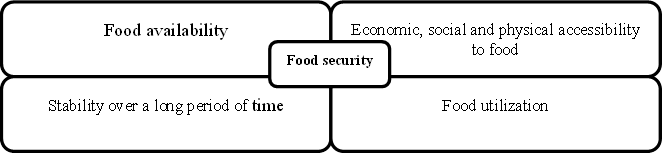
\includegraphics[width=4.64317in,height=4.95932in]{media/image2.png}

\textbf{Fig. 1- The algorithm of the program code}

\emph{\textbf{The algorithm works as follows:}}

Data for each ingredient of the construction mix with additives of
man-made raw materials is uploaded from the interface.

\textbf{1. Data initialization:}

The main() function sets the parameters for calculating the construction
mix:

-the volume of the mixture (volume) in m\textsuperscript{3};

-the density of the material (Material Densities) in kg /
m\textsuperscript{3};

-the percentage of the material (Material percentages);

-material costs (cost) per 1 kg.

\begin{enumerate}
\def\labelenumi{\arabic{enumi}.}
\setcounter{enumi}{1}
\item
  \textbf{Mix Composition Calculation:}
\end{enumerate}

-the function calculate\_concrete\_mix(volume, densities, percentages,
costs) is called:

-a list to store mix composition data and a variable for the total cost
are initialized. For each ingredient;

\begin{quote}
The function returns:

-a list of data for the mix composition;

-the total cost of the mix.
\end{quote}

Updating data on cost, density of materials, and adding new materials is
carried out using artificial intelligence.

\begin{quote}
\textbf{3. Saving Results to Excel:}

the function save\_to\_excel(data, file\_path) performs:

-creates an Excel file;

-adds table headers;

-writes rows containing mix composition data.

Formats the table:

-adjusts column widths;

-highlights headers with bold text and centers the text;
\end{quote}

-sets the print area, page orientation, and scaling to fit the table to
one page width.

\begin{quote}
Saves the file to the specified path.

\textbf{4. Result Display:}

After saving the file, the program outputs:

-the path to the Excel file;

-the total cost of the construction mix.

\textbf{5. Program Execution:}

the program checks if it is the main module (if \_\_name\_\_ ==
"\_\_main\_\_":);
\end{quote}

the main() function is called to perform the calculations and save the
results.

Fig. 2-11 show the program code of the program "Automated system for
selecting the composition of a building mix with additives from man-made
raw materials."

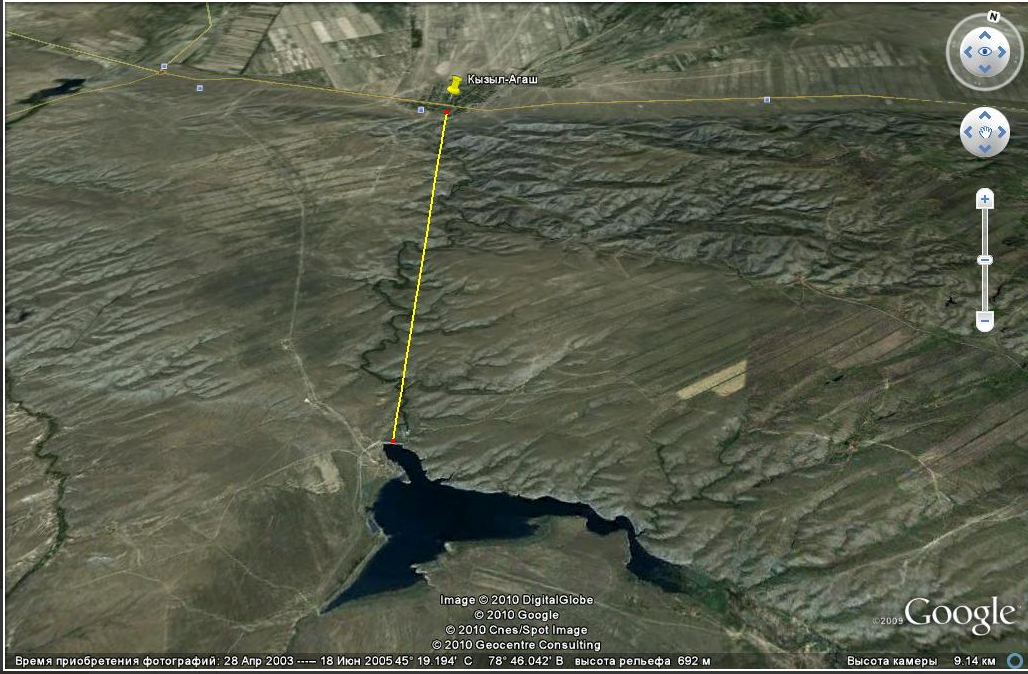
\includegraphics[width=5.64832in,height=2.48442in]{media/image3.png}

\textbf{Fig. 2-Program code (Data entry)}

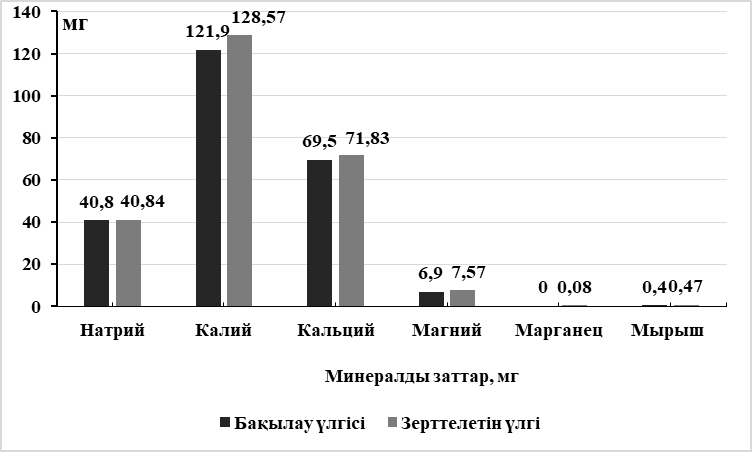
\includegraphics[width=6in,height=1.73648in]{media/image4.png}

\textbf{Fig/ 3-Program code (Verification of compliance with the
percentage of the building mix)}

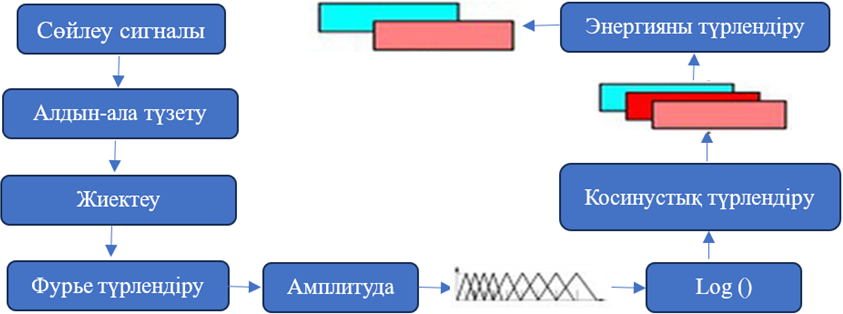
\includegraphics[width=5.51042in,height=1.03156in]{media/image5.png}

\textbf{Fig. 4-Program code (Functions for determining the density and
cost of the material)}


\includegraphics[width=5.26042in,height=2.34981in]{media/image6.png}

\textbf{Fig. 5- Program code (Calculation)}

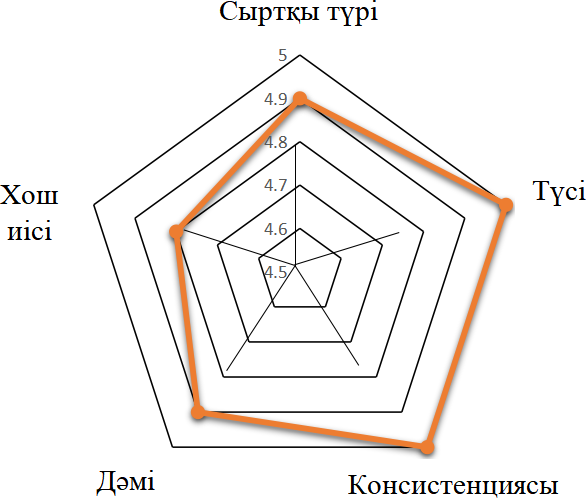
\includegraphics[width=5.125in,height=2.50398in]{media/image7.png}

\textbf{Fig. 6-Program code (Updating ingredients using AI)}

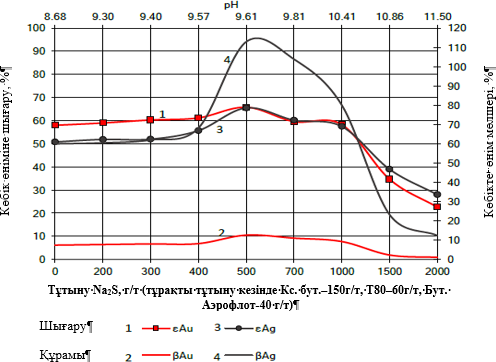
\includegraphics[width=5.26042in,height=2.30275in]{media/image8.png}

\textbf{Fig. 7- Program code (Updating the density of the material using
AI)}

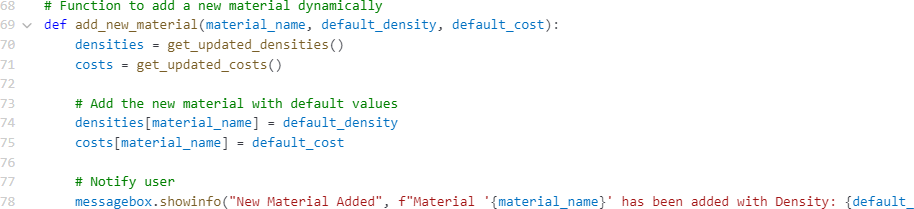
\includegraphics[width=4.98958in,height=2.11575in]{media/image9.png}

\textbf{Fig. 8-Program code (Adding new materials)}

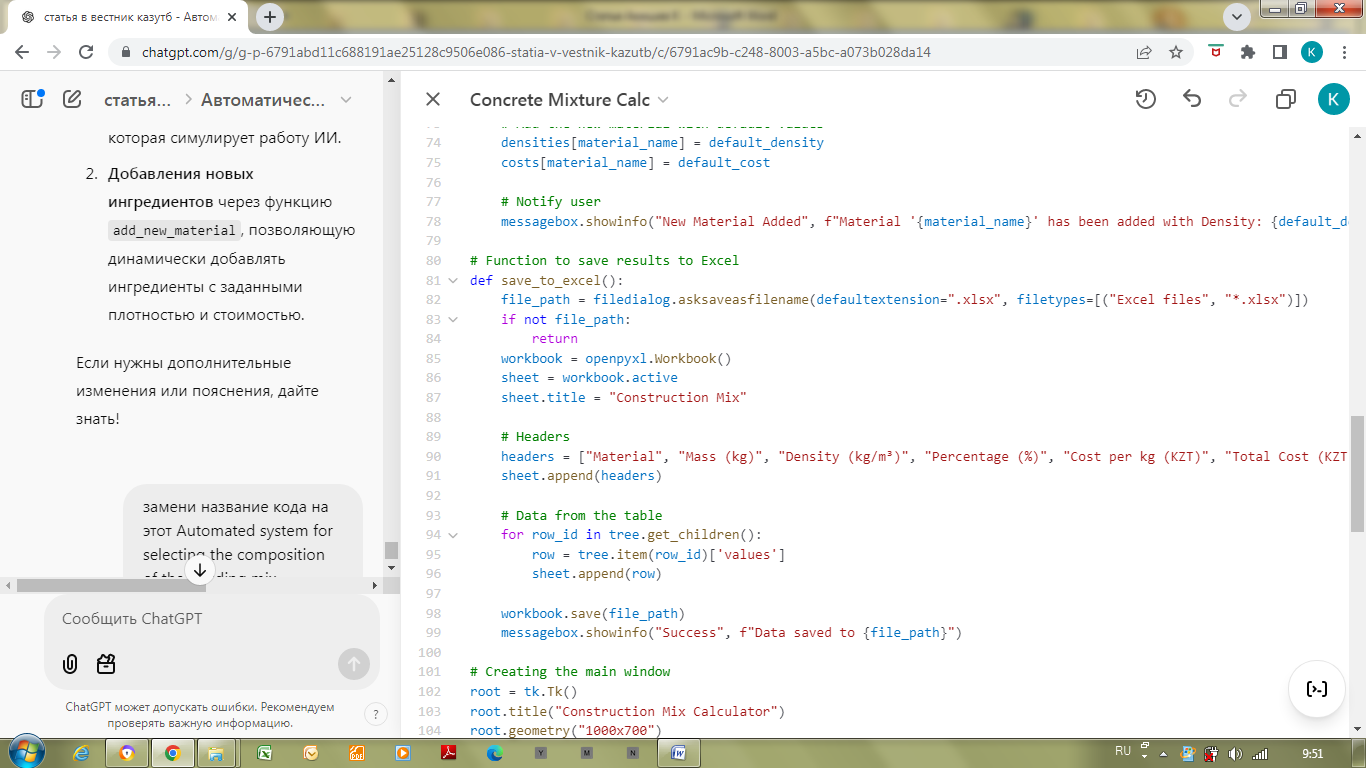
\includegraphics[width=5.11458in,height=1.56273in]{media/image10.png}

\textbf{Fig. 9-Program code (Conversion of calculation results to
Excel)}

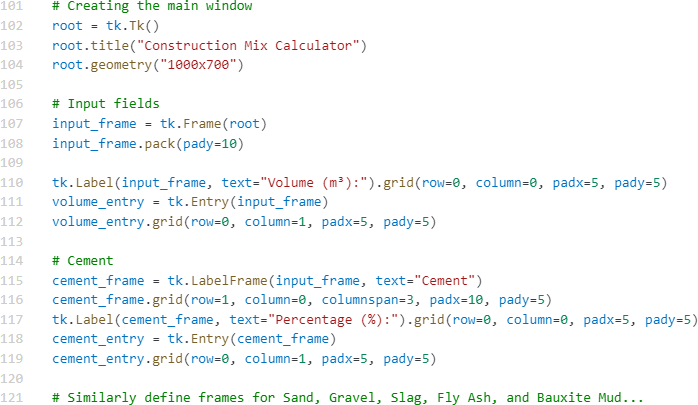
\includegraphics[width=5.47917in,height=2.10417in]{media/image11.png}

\textbf{Fig. 10-Program code (Creating windows)}

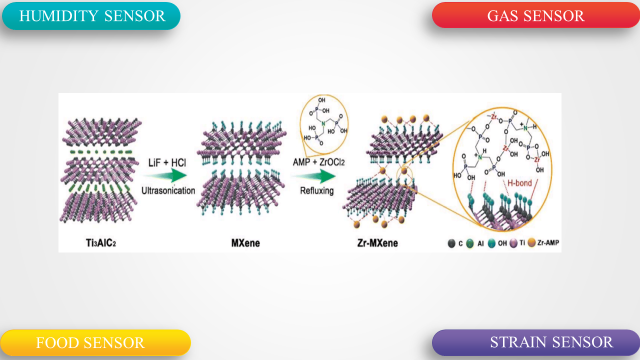
\includegraphics[width=4.82292in,height=0.8125in]{media/image12.png}

\textbf{Fig. 11-Program code (program launch)}

Figure 12 shows the menu interface of the program "Automated system for
selecting the composition of a building mix with additives from man-made
raw materials."

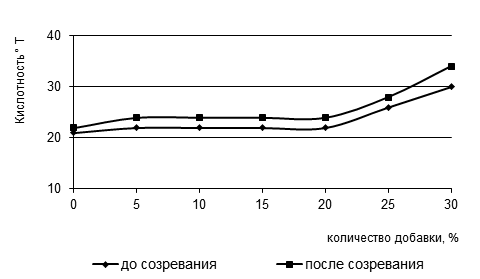
\includegraphics[width=5.7001in,height=2.96512in]{media/image13.png}

\textbf{Fig. 12- Menu interface of the program "Automated system for
selecting the composition of}

\textbf{a building mix with additives from man-made raw materials"}

User interaction with the program

1. Program launch:

the user launches the file. A window opens with fields for data entry.

2. Data entry:

The user enters:

the volume of the mixture (m3);

the percentage of each ingredient.

If necessary, you can add new ingredients.

3. Performing the calculation:

-clicking on the "Calculate" button starts the calculation.

Saving the results:

-the user clicks the "Save to Excel" button to save the results to a
file.

4. Adding new ingredients:

with the "Add Material" button, the user adds the ingredients that need
to be used in calculations.

Program operation:

The user enters:

Volume: 1 m3.

-cement: 13\%;

- sand: 15\%;

-Crushed stone: 50\%;

-slag: 10\%;

-fly ash: 7\%;

-Bauxite sludge: 5\%.

Presses the "Calculate" button. The program:

-verifies the correctness of the data;

-calculates the mass and cost of each ingredient.

-Determines the total cost of the construction mix depending on the
percentage composition.

Clicks "Save to Excel":

The program:

creates an Excel file and saves the data.

The results of calculating the selection of the building mix are
presented in Table 1.

\textbf{Table 1- The results of calculating the selection of the
building mix}

\begin{longtable}[]{@{}
  >{\raggedright\arraybackslash}p{(\columnwidth - 10\tabcolsep) * \real{0.1495}}
  >{\raggedright\arraybackslash}p{(\columnwidth - 10\tabcolsep) * \real{0.1648}}
  >{\raggedright\arraybackslash}p{(\columnwidth - 10\tabcolsep) * \real{0.1692}}
  >{\raggedright\arraybackslash}p{(\columnwidth - 10\tabcolsep) * \real{0.1846}}
  >{\raggedright\arraybackslash}p{(\columnwidth - 10\tabcolsep) * \real{0.1473}}
  >{\raggedright\arraybackslash}p{(\columnwidth - 10\tabcolsep) * \real{0.1846}}@{}}
\toprule\noalign{}
\begin{minipage}[b]{\linewidth}\raggedright
Material
\end{minipage} & \begin{minipage}[b]{\linewidth}\raggedright
Percentage (\%)
\end{minipage} & \begin{minipage}[b]{\linewidth}\raggedright
Density (kg/m³)
\end{minipage} & \begin{minipage}[b]{\linewidth}\raggedright
Cost per kg (KZT)
\end{minipage} & \begin{minipage}[b]{\linewidth}\raggedright
Mass (kg)
\end{minipage} & \begin{minipage}[b]{\linewidth}\raggedright
Total Cost (KZT)
\end{minipage} \\
\midrule\noalign{}
\endhead
\bottomrule\noalign{}
\endlastfoot
Cement & 13 & 1400 & 200 & 182 & 36400 \\
Sand & 15 & 1600 & 30 & 240 & 7200 \\
Gravel & 50 & 1500 & 50 & 750 & 37500 \\
Slag & 10 & 1200 & 80 & 120 & 9600 \\
Fly Ash & 7 & 800 & 70 & 56 & 3920 \\
Bauxite Mud & 5 & 1000 & 100 & 50 & 5000 \\
\end{longtable}

If necessary, the user can add a new ingredient by clicking the "Add
Material" button. Table 2 shows the calculation results for the
percentage composition with other numerical values.

\textbf{Table 2- Results of calculating the selection of the
construction mixture}

\begin{longtable}[]{@{}
  >{\raggedright\arraybackslash}p{(\columnwidth - 10\tabcolsep) * \real{0.1563}}
  >{\raggedright\arraybackslash}p{(\columnwidth - 10\tabcolsep) * \real{0.1783}}
  >{\raggedright\arraybackslash}p{(\columnwidth - 10\tabcolsep) * \real{0.1629}}
  >{\raggedright\arraybackslash}p{(\columnwidth - 10\tabcolsep) * \real{0.1739}}
  >{\raggedright\arraybackslash}p{(\columnwidth - 10\tabcolsep) * \real{0.1651}}
  >{\raggedright\arraybackslash}p{(\columnwidth - 10\tabcolsep) * \real{0.1636}}@{}}
\toprule\noalign{}
\begin{minipage}[b]{\linewidth}\raggedright
Material
\end{minipage} & \begin{minipage}[b]{\linewidth}\raggedright
Percentage (\%)
\end{minipage} & \begin{minipage}[b]{\linewidth}\raggedright
Density (kg/m³)
\end{minipage} & \begin{minipage}[b]{\linewidth}\raggedright
Cost per kg (KZT)
\end{minipage} & \begin{minipage}[b]{\linewidth}\raggedright
Mass (kg)
\end{minipage} & \begin{minipage}[b]{\linewidth}\raggedright
Total Cost (KZT)
\end{minipage} \\
\midrule\noalign{}
\endhead
\bottomrule\noalign{}
\endlastfoot
Cement & 14 & 1400 & 200 & 196 & 39200 \\
Sand & 16 & 1600 & 30 & 256 & 7680 \\
Gravel & 40 & 1500 & 50 & 600 & 30000 \\
Slag & 15 & 1200 & 80 & 180 & 14400 \\
Fly Ash & 10 & 800 & 70 & 80 & 5600 \\
Bauxite Mud & 5 & 1000 & 100 & 50 & 5000 \\
\end{longtable}

The program code has the ability to analyze data for different building
mix compositions. In particular, Fig. 13 shows a graph of the effect of
the percentage of man-made raw materials and building mixes on its cost.


\includegraphics[width=4.88317in,height=1.841in]{media/image14.png}

\textbf{Fig. 13- Graph of the effect of the percentage composition of
the building mix on its cost}

As can be seen from the graph, when the composition of man-made raw
materials reaches 15\%, there is a significant reduction in the cost of
the construction mixture.

If necessary, various types of analysis can be obtained related to the
study of building mixes obtained as a result of automated selection.

\textbf{Conclusion.} The proposed development methodology and the
developed program code are based on a flexible and modular approach that
allows automating the selection of building mixes using man-made raw
materials.

The scientific approach of the proposed methodology is based on:

- the use of mathematical modeling methods that ensure high accuracy of
calculations;

- realization of artificial intelligence capabilities for updating
information data;

-obtaining data analysis based on graphical representation of the
results of calculating the composition of the construction mixture with
additives of man-made raw materials.

The scientific novelty of the developed program consists in the
development of an original algorithm and the absence of analogues of the
source code, which allows obtaining both practical and scientific
results.

The developed program "Automated system for selecting the composition of
a building mix with additives from man-made raw materials" can be used
for practical purposes in business processes, small and medium-sized
businesses, during scientific experiments (master\textquotesingle s
degree, doctoral studies), in the educational process of the educational
program "Information Technology", Automation and Control, "Building
Materials".

The effectiveness of the developed program is incomparable with the
manual selection of a building mix and takes this process to a new
level.

\textbf{Referenses}

1.Аkishev K. Inzhenernoe modelirovanie clozhnikh tekhnologicheskikh
sistem (proizvodstvo stroitelnikh izdelii s ispolzovanien tekhnogennikh
otkhodov. {[}Engineering modeling of complex technological systems
(production of construction products using man-made waste){]}. Lantar
books Publishing House, Almaty, 2023.-142s, 500 copies. ISBN
978-601-361-254-6 {[}in Russian{]}

2. Аkishev K and other\textbf{.} Тhe use of simulation modeling in
calculating the productivity of the technological system for the
production of building products with fillers from man-made waste// NEWS
of the National Academy of Sciences of the Republic of Kazakhstan.-
Series of geology and technical sciences.-2024.-Vol. 4. (466)- P.
22--32. \href{https://doi.org/10.32014/2024.2518-170X.422}{DOI
10.32014/2024.2518-170X.422}

\paragraph{\texorpdfstring{3. Аkishev K and other. Еvaluation of the
efficiency of the technological process for the production of building
products with fillers from metallurgical
slag//\emph{Metalurgija}.-2024.-63(2).- P. 267--27.
}{3. Аkishev K and other. Еvaluation of the efficiency of the technological process for the production of building products with fillers from metallurgical slag//Metalurgija.-2024.-63(2).- P. 267--27. }}\label{ux430kishev-k-and-other.-ux435valuation-of-the-efficiency-of-the-technological-process-for-the-production-of-building-products-with-fillers-from-metallurgical-slagmetalurgija.-2024.-632.--p.-26727.}

4. Аkishev K and other\emph{\textbf{.}} Information technologies in the
management of technological processes for the production of building
products\emph{//} Eastern-European Journal of Enterprise
Technologies\emph{.-~}2024.- 1(2(127).-P. 66--73.
\href{https://doi.org/10.15587/1729-4061.2024.298480}{DOI
10.15587/1729-4061.2024.298480}

5. Chetan G. Kanapure and other. Interdisciplinary Approaches to AI,
Internet of Everything, and Machine Learning (2024).-рp.567-586).
-Artificial Intelligence in Automated Concrete Mix Design Using
Computerized Grading Curves\textbf{.}
DOI\href{http://dx.doi.org/10.4018/979-8-3373-1032-9.ch036}{10.4018/979-8-3373-1032-9.ch036}

6. Vasileios Sergis, Claudiane M. Automating Mix Design for 3D Concrete
Printing Using Optimization Methods.- Digital
Discovery.-2022.-Vol.1(7).-P. 645-657.
\href{https://doi.org/10.1039/D2DD00040G}{DOI 10.1039/D2DD00040G}

7. Yaser Gamil and other. Frontier in Builit EnvironmentDigital
Transformation of Concrete Technology --A Review. -Sec/ Sustainable
Design and Constraction. -2022.-Vol.8
\href{https://doi.org/10.3389/fbuil.2022.835236}{DOI
10.3389/fbuil.2022.835236}

8.Jessica C. Forsdyke and other. Probabilistic Selection and Design of
Concrete Using Machine Learning// Data-Centric Engineering.-
2023.-Vol.4. DOI 10.1017/dce.2023.5

9\textbf{.} Atul Agrawal and other. From Concrete Mixture to Structural
Design-A Holistic Optimization Procedure in the Presence of
Uncertainties.// Data-centric-engineering.-2023.e20.
\href{https://doi.org/10.1017/dce.2024.18}{DOI 10.1017/dce.2024.18}

9. Atul Agrawal and other. Data-centric-engineering.(2023) "From
Concrete Mixture to Structural Design---A Holistic Optimization
Procedure in the Presence of Uncertainties" . Начало формы

\section{10.Anna Corolina Rosa and other. Use of Operational Research
Techniques for Concrete Mix Design:A systematic review.// Heliyon.-
2023.-Vol.9(4):e15362}\label{anna-corolina-rosa-and-other.-use-of-operational-research-techniques-for-concrete-mix-designa-systematic-review.-heliyon.--2023.-vol.94e15362}

\href{https://doi.org/10.1016/j.heliyon.2023.e15362}{DOI
10.1016/j.heliyon.2023.e15362}

\section{11. Haidong Tu and other. 16 (2023) . Recent advancements and
future trends in 3D concrete printing using waste materials//
Developments in the Built
Environment.-2023.-Vol.16;100187}\label{haidong-tu-and-other.-16-2023-.-recent-advancements-and-future-trends-in-3d-concrete-printing-using-waste-materials-developments-in-the-built-environment.-2023.-vol.16100187}

\section{\texorpdfstring{\href{https://doi.org/10.1016/j.dibe.2023.100187}{DOI
10.1016/j.dibe.2023.100187}}{DOI 10.1016/j.dibe.2023.100187}}\label{doi-10.1016j.dibe.2023.100187}

12. Egor Popello, Victoria GurievAutomation of the concrete mix
preparation process as a means to improve production efficiency//Matec
Web of Conferences.-2017.-Vol.129: 05003

DOI
\href{http://dx.doi.org/10.1051/matecconf/201712905003}{10.1051/matecconf/201712905003}

13. S. Barbhuiya.Artificial Intelligence in Concrete Mix Design:
Advances, Applications, and Challenges, 2023 International Conference on
Innovation and Intelligence for Informatics, Computing, and Technologies
(3ICT). \href{http://dx.doi.org/10.1109/3ICT60104.2023.10391485}{DOI
10.1109/3ICT60104.2023.10391485}

14. Max Coenen and other. "Computer Vision as Key to an Automated
Concrete Production Control.2024.- P.26-33. Proceedings of the 41st
ISARC, Lille, France. ISBN 978-0-6458322-1-1, ISSN 2413-5844.
\href{https://doi.org/10.22260/ISARC2024/0005}{DOI
10.22260/ISARC2024/0005}

15. Santalova М.S., Soklakova I. V., Gorlov V.V., Muza U.А.
Avtomatizaciya proektnikh rabot v stroitelnoi kompanii v usloviyakh
cifrovizacii// Cifrivaya ekonomika.-2021.-Т.14.№2(53).-S.51-57. DOI
10.29030/2309-2076-2021-14-2-21-57. {[}in Russian{]}

\emph{\textbf{Information about the authors}}

Akishev K. M. - Candidate of Technical Sciences, Ass. Professor, Kazakh
University of Technology and Business named after K. Kulazhanov, Astana,
Kazakhstan, e -mail:akmail04cx@mail.ru;

Tulegulov A. D.- Candidate of physics and mathematics Sciences, Ass.
Professor, Kazakh University of Technology and Business named after. K.
Kulazhanov,Astana, Kazakhstan,e-mail:tud62@yandex.ru;

Nurtai Z.T. - Ph.D., Ass. Professor, Kazakh University of Technology and
Business named after. K. Kulazhanov,Astana, Kazakhstan, e-mail:
zhadira\_nurtai@mail.ru;

Akisheva L.- Nazarbayev Intellectual School, Astana, Republic of
Kazakhstan, e-mail: L. \href{mailto:Ak@mail.ru}{\nolinkurl{Ak@mail.ru}};

Biybosunov B.I.-Doctor of Physico-mathematical Sciences, Doctor of
Technical Sciences, Professor, Kyrgyz State University named after I.
Arabaev, Bishkek, Kyrgyzstan, e-mail: b.biibosunov@mail.ru;

Baizharikova M.M.-Candidate of Technical Sciences, Associate Professor,
Taraz Regional University, Taraz, Kazakhstan, e-mail:marina2288@mail.ru

\emph{\textbf{Информация об авторах}}

Акишев К. М. -к.т.н., асс. профессор, Казахский университет технологии и
бизнеса им. К. Кулажанова, Астана, Казахстан, e-mail:akmail04cx@mail.ru;

Нуртай Ж.Т. - доктор PhD, асс. профессор, Казахский университет
технологии и бизнеса им. К. Кулажанова,

Астана, Казахстан, e-mail: zhadira\_nurtai@mail.ru

Акишева Л. -Назарбаев интеллектуальная школа, г. Астана, Казахстан,
e-mail: L.Ak@mail.ru;

Тулегулов А. Д.- к.ф.м.н., асс. профессор, Казахский университет
технологии и бизнеса им. К.Кулажанова, Астана, Казахстан:
e-mail:tud62@yandex.ru;

Бийбосынов Б.И.-д.ф.-м.н, д.т.н., профессор, Кыргызский Государственный
университет им. И. Арабаева, Бишкек, Кыргызстан,
e-mail:b.biibosunov@mail.ru;

Байжарикова М.М.-к.т.н., ассоциированный профессор, Таразский
Региональный университет, Тараз, Казахстан, e-mail: marina2288@mail.ru

МРНТИ 28.17.19

ПРОГНОЗИРОВАНИЕ ПОСЛЕДСТВИЙ СЕЛЕВОГО ПРОРЫВА С УЧЕТОМ ХАРАКТЕРИСТИК
ВОДОЕМА

\textsuperscript{1}А.Т.
Мазакова
\includegraphics[width=0.14722in,height=0.14722in]{media/image1.png},
\textsuperscript{1}Ш.А.
Джомартова
\includegraphics[width=0.14722in,height=0.14722in]{media/image1.png},
\textsuperscript{2}Б.М.
Мазакова
\includegraphics[width=0.14722in,height=0.14722in]{media/image1.png},
\textsuperscript{3} М.С.
Алиаскар
\includegraphics[width=0.14722in,height=0.14722in]{media/image1.png},

\textbf{\textsuperscript{1}Е.К.
Мергенгали}
\includegraphics[width=0.14722in,height=0.14722in]{media/image1.png}\textbf{,
\textsuperscript{1,3}Т.Ж.
Мазаков\textsuperscript{🖂}}
\includegraphics[width=0.14722in,height=0.14722in]{media/image1.png}\textbf{,
\textsuperscript{4} А.Т.
Досаналиева}
\includegraphics[width=0.14722in,height=0.14722in]{media/image1.png}
,
\textbf{\textsuperscript{5}А.Д.Майлыбаева}
\includegraphics[width=0.15in,height=0.15in]{media/image1.png}

\emph{¹Казахский национальный университет имени аль-Фараби, Алматы,
Казахстан,}

\emph{\textsuperscript{2}Казахский агротехнический исследовательский
университет имени С. Сейфуллина, Астана, Казахстан,}

\emph{\textsuperscript{3}Международный инженерно-технологический
университет, Алматы, Казахстан,}

\emph{\textsuperscript{4}Алматинский Технологический Университет,
Алматы, Казахстан,}

\emph{\textsuperscript{5}Атырауский универститет имени Х. Досмухамедова}

\textbf{\textsuperscript{🖂}}Корреспондент-автор: tmazakov@mail.ru

Весной 2010 года в Алматинской области, в 2014 году в Карагандинской
области, а также в начале 2024 года в северных регионах Казахстана
произошли разрушительные наводнения, сопровождавшиеся человеческими
жертвами и значительным ущербом. Эти события подчеркнули необходимость
создания эффективных систем мониторинга для гидротехнических сооружений.

Современные системы мониторинга гидрологической ситуации на водоемах
позволяют заранее выявлять потенциальные угрозы для человека и
окружающей среды. Основная цель мониторинга заключается в предоставлении
точных данных, необходимых для прогнозирования чрезвычайных ситуаций.
Проектирование таких систем включает разработку и анализ математических
моделей, способных в режиме реального времени рассчитывать объем воды,
который может вместить водоем, а также предсказывать момент его
заполнения и угрозы прорыва плотины. Применение таких систем
способствует принятию оперативных мер по обеспечению экологической
безопасности.

В данной работе представлена система прогнозирования, способная
оценивать последствия селевых прорывов. Разработанная система базируется
на методах математического моделирования. В отличие от аналогов,
предложенная модель учитывает, как параметры водоема, так и особенности
русла реки.

Для внедрения системы в практику создано программное обеспечение на
языке Python. Проведенные эксперименты показали, что модель достоверно
отражает реальные условия и может успешно применяться в различных
сценариях.

\textbf{Ключевые слова:} бьеф, математическая модель, плотина,
прогнозирование, сель.

СУ ОБЪЕКТІНІҢ СИПАТТАРЫН ЕСКЕ АЛУ МЕН СЕЛДІҢ САЛДАРЫН БОЛЖАУ

\textsuperscript{1}Ә.Т. Мазақова, \textsuperscript{1}Ш.А. Джомартова,
\textsuperscript{2}Б.М. Мазакова, \textsuperscript{3}М.С. Әлиасқар,

\textsuperscript{1}Е.К. Мергенгали, \textsuperscript{1,3}Т.Ж. Мазақов,
\textsuperscript{4} А.Т. Досаналиева, \textsuperscript{5}А.Д.Майлыбаева

\emph{¹Әл-Фараби атындағы Қазақ ұлттық университеті, Алматы, Қазақстан,}

\emph{²Сейфуллин атындағы Қазақ агротехникалық зерттеу университеті,
Астана, Қазақстан,}

\emph{\textsuperscript{3}Халықаралық инженерлік және технология
университеті, Алматы, Қазақстан,}

\emph{\textsuperscript{4}Алматы технологиялық университеті, Алматы,
Қазақстан,}

\emph{\textsuperscript{5}Досмұхамедов атындағы Атырау университеті,}

\emph{e-mail:} \emph{tmazakov@mail.ru}

2010 жылдың көктемінде Алматы облысында, 2014 жылы Қарағанды
\hspace{0pt}\hspace{0pt}облысында, ал 2024 жылдың басында Қазақстанның
солтүстік облыстарында адам шығынымен және айтарлықтай шығынмен қатар
жүретін жойқын су тасқыны болды. Бұл іс-шаралар гидротехникалық
құрылыстарды бақылаудың тиімді жүйелерінің қажеттілігін көрсетті.

Су объектілеріндегі гидрологиялық жағдайды бақылаудың заманауи жүйелері
адам мен қоршаған ортаға ықтимал қауіптерді алдын ала анықтауға
мүмкіндік береді. Мониторингтің негізгі мақсаты -- төтенше жағдайларды
болжауға қажетті нақты мәліметтерді қамтамасыз ету. Мұндай жүйелерді
жобалау нақты уақыт режимінде резервуар ұстай алатын су көлемін
есептеуге, сондай-ақ оны толтыру сәтін және бөгеттің бұзылу қаупін
болжауға қабілетті математикалық модельдерді әзірлеуді және талдауды
қамтиды. Мұндай жүйелерді пайдалану экологиялық қауіпсіздікті қамтамасыз
ету бойынша жедел шараларды қабылдауға ықпал етеді.

Бұл жұмыста селдің салдарын бағалауға қабілетті болжау жүйесі ұсынылған.
Әзірленген жүйе математикалық модельдеу әдістеріне негізделген. Өзінің
аналогтарынан айырмашылығы, ұсынылған модель су қоймасының параметрлерін
де, өзен арнасының ерекшеліктерін де ескереді.

Жүйені тәжірибеге енгізу үшін Python тілінде бағдарламалық жасақтама
жасалды. Жүргізілген эксперименттер модель нақты жағдайларды сенімді
түрде көрсететінін және әртүрлі сценарийлерде сәтті қолданыла алатынын
көрсетті.

\textbf{Түйін сөздер:} бассейн, математикалық модель, бөгет, болжау,
сел.

\textbf{FORECASTING THE CONSEQUENCES OF A MUDFLOW TAKING INTO ACCOUNT
THE CHARACTERISTICS OF THE WATER BODY}

\textsuperscript{1}A.T. Mazakova, \textsuperscript{1}Sh.A. Jomartova,
²B.M. Mazakova, \textsuperscript{3}M.S. Aliaskar,

\textsuperscript{1}Y.К. Mergengali, \textsuperscript{1,3}T.Zh. Mazakov,
\textsuperscript{4}A.T.Dossanalyieva, \textsuperscript{5}A.D.Mailybayeva

\emph{¹Kazakh National University named after Al-Farabi, Almaty,
Kazakhstan,}

\emph{\textsuperscript{2}Kazakh Agrotechnical Research University named
after S. Seifullin, Astana, Kazakhstan,}

\emph{\textsuperscript{3}International Engineering and Technology
University, Almaty, Kazakhstan,}

\emph{\textsuperscript{4}Almaty Technological University, Almaty,
Kazakhstan,}

\begin{quote}
\emph{\textsuperscript{5}Atyrau University named after Kh.
Dosmukhambetov,}
\end{quote}

\emph{e-mail:} \emph{tmazakov@mail.ru}

In the spring of 2010 in the Almaty region, in 2014 in the Karaganda
region, and in early 2024 in the northern regions of Kazakhstan,
devastating floods occurred, accompanied by human casualties and
significant damage. These events emphasized the need to create effective
monitoring systems for hydraulic structures.

Modern systems for monitoring the hydrological situation on water bodies
allow early detection of potential threats to humans and the
environment. The main goal of monitoring is to provide accurate data
necessary for forecasting emergency situations. Designing such systems
includes the development and analysis of mathematical models capable of
calculating in real time the volume of water that a water body can hold,
as well as predicting the moment of its filling and the threat of a dam
break. The use of such systems facilitates the adoption of prompt
measures to ensure environmental safety.

This paper presents a forecasting system capable of assessing the
consequences of mudflows. The developed system is based on mathematical
modeling methods. Unlike analogues, the proposed model takes into
account both the parameters of the reservoir and the features of the
river bed.

To implement the system in practice, software was created in Python. The
experiments showed that the model reliably reflects real conditions and
can be successfully applied in various scenarios.

\textbf{Keywords:} pool, mathematical model, weir, forecasting, mudflow.

\textbf{Актуальность.} За последнее столетие в мире произошло множество
катастроф, связанных с разрушением гидротехнических сооружений, которые
сопровождались человеческими жертвами и значительными экономическими
потерями.

Одной из наиболее трагических стала авария на плотине Сент-Франсис в
Калифорнии, произошедшая в марте 1928 года, когда погибло более 600
человек. В 1963 году обрушение горного массива в водохранилище Вайонт
(Италия) вызвало гигантские волны высотой до 70 метров, которые
разрушили четыре населенных пункта и привели к гибели 4400 человек.
Наводнение в Краснодарском крае в июле 2002 года, повлекшее разрушение
гидроузла, стало причиной гибели 114 тысяч человек и нанесло
экономический ущерб, оцененный в 15 миллиардов рублей {[}1-2{]}.

17 августа 2009 года на Саяно-Шушенской ГЭС произошла крупная авария,
унесшая жизни 75 человек. В результате были серьезно повреждены
оборудование и инфраструктура станции. Авария вызвала негативные
изменения в экологической ситуации прилегающей акватории, а также
оказала значительное влияние на социально-экономическое состояние
региона и страны в целом {[}3{]}.

Современные мониторинговые системы должны обеспечивать постоянное
наблюдение за природными и техногенными процессами, чтобы заранее
выявлять потенциальные угрозы для жизни человека и окружающей среды.
Основная задача мониторинга заключается в предоставлении точной
информации, необходимой для прогнозирования чрезвычайных ситуаций. Для
этого необходимо объединять интеллектуальные, информационные и
технологические ресурсы различных организаций и ведомств, отвечающих за
мониторинг специфических опасностей.

Проектирование мониторинговых систем требует разработки и анализа
математических моделей, способных в реальном времени определять объем
воды, который может вместить водоем, а также прогнозировать время до его
заполнения (до уровня гребня плотины). Эти данные являются критически
важными для своевременного предупреждения населения и органов власти,
что позволяет оперативно принимать меры по обеспечению экологической
безопасности.

Таким образом, исследования, направленные на разработку математических
моделей для оценки прорыва дамб и создание надежных средств защиты
информации, остаются весьма актуальными.

\textbf{Введение.} В Казахстане насчитывается 1665 гидротехнических
сооружений, включая 319 водохранилищ объемом более 1,0 млн м³. Из них в
республиканской собственности находится 83 объекта, в коммунальной --
200, в частной -- 34, а 60 водохранилищ являются бесхозяйными. Среди 443
плотин 32 находятся в республиканской собственности, 346 -- в
коммунальной, 45 -- в частной, а 20 остаются бесхозяйными. Также
эксплуатируются 125 дамб и 778 других гидротехнических сооружений.

Среди крупных водохранилищ выделяются Астанинское (1970 г., объем 410,9
млн м³), Селетинское (1965 г., 230 млн м³), Каргалинское (1975 г., 280
млн м³), Бартогайское (1982 г., 320 млн м³), Капшагайское (1970 г., 18
560 млн м³), Терс-Ащибулакское (1963 г., 158,6 млн м³), Тасоткельское
(1974 г., 620 млн м³), Самаркандское (1939 г., 253,7 млн м³),
Верхне-Тобольское (1972 г., 816,6 млн м³), Каратомарское (1965 г., 586
млн м³), Бугуньское (1967 г., 370 млн м³) и другие.

Большинство водохранилищ и гидроузлов (около 60\%) находятся в
коммунальной собственности, в том числе на балансе Казводхоза, а около
20\% объектов принадлежат отделам сельского хозяйства акиматов. Эта
ситуация указывает на нерешенность вопроса об окончательной
принадлежности данных объектов. В течение последних 10--15 лет около
20\% водохранилищ были переданы в аренду частным лицам, преимущественно
для нужд сельского хозяйства, рыбоводства и рекреации. Однако только в
отдельных случаях аренда приносит положительные результаты, поскольку
частным арендаторам часто не хватает средств для ремонта ключевых
сооружений {[}4{]}.

Весной 2010 года в Алматинской области произошло разрушительное
наводнение, вызванное прорывом плотины, повлекшее человеческие жертвы и
масштабные разрушения. Подобное трагическое событие повторилось в 2014
году в Карагандинской области. Эти катастрофы стали серьезным
предупреждением для страны и подчеркнули важность предотвращения таких
ситуаций в будущем {[}5{]}.

\textbf{Материалы и методы.} В математической модели рассмотрен
трапецеидальный тип водоема, вид которого со стороны плотины представлен
на рисунке 1.

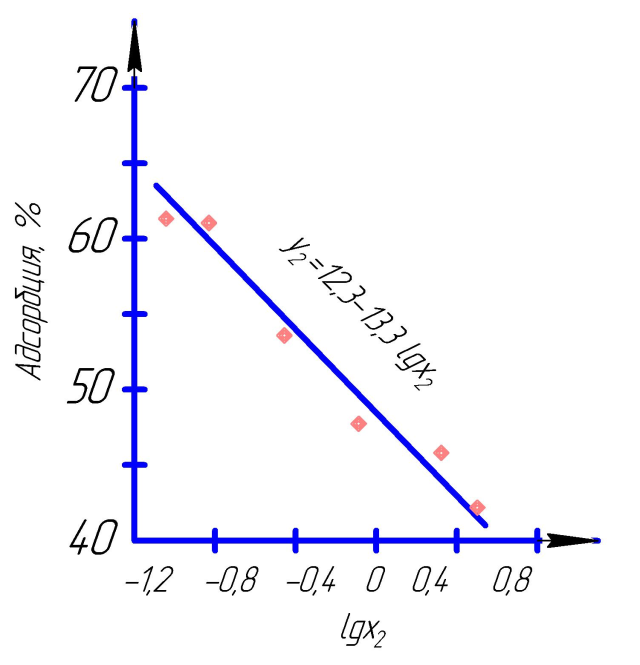
\includegraphics[width=2.21875in,height=1.79167in]{media/image15.png}\\
\textbf{Рис. 1- Вид водоема со стороны плотины}

Введем следующие обозначения {[}6-8{]}:

\(\mathrm{\Delta}T\)- временной шаг отсчета (в часах);

\(l\) - длина водоема (в метрах)

\(\omega_{0}\) , \(S_{0}\) - ширина и площадь водоема по основанию;

\(\omega_{1}\) , \(S_{1}\) - ширина и площадь водоема по уровню гребня
плотины;

\(\omega_{2}\) , \(S_{2}\) - ширина и площадь водоема по поверхности
воды;

\(\omega_{3}\) , \(S_{3}\) - ширина и площадь водоема по верхней точки
прорана в плотине;

\(V_{0}\) -- общий объем водоема;

\(V_{1}\) -- незаполненный объем водоема;

\(V_{2}\) -- объем водоема от поверхности воды до верхней точки прорана
в плотине;

\(V_{3}\) -- объем водоема от нижней до верхней точки прорана в плотине;

\(\mathrm{\Delta}V_{1}\) - объем воды поступившей в водоем за время
\(\mathrm{\Delta}T\);

\(\mathrm{\Delta}V_{2}\) - объем воды вытекший из водоема за время
\(\mathrm{\Delta}T\);

\(\mathrm{\Delta}V\) - разница между объемами вытекшей и поступившей
воды за время \(\mathrm{\Delta}T\);

\(h_{0}\)- высота плотины;

\(h_{1}\) - расстояние от гребня плотины до поверхности воды;

\(h_{2}\)- расстояние от поверхности воды до верхней точки прорана в
плотине;

\(h_{pr}\) - высота прорана в плотине;

\(\omega_{pr}\)- ширина прорана в плотине.

Так как параметры \(h_{0}\) , \(h_{pr}\) являются постоянными, \(h_{1}\)
и \(h_{2}\) изменяются по времени, то введем обозначения \(h_{1,k}\) и
\(h_{2,k}\) , где индекс к означет значение соответствующего параметра в
момент времени \(T_{k}\).

Тогда справедливы формулы

\(h_{0} - h_{pr} = h_{1,k} + h_{2,k}\),
\(V_{0} - V_{3} = V_{1,k} + V_{2,k}\) (1)

Длина водоема \(l\) , ширина водоема по основанию \(\omega_{0}\ \)и
гребню плотины \(\omega_{1}\), высота \(h_{0}\), ширина и высота прорана
\(h_{pr}\ \), \(\omega_{pr}\) известны и являются постоянными. Также
предполагается постоянным объем воды \(\mathrm{\Delta}V_{1}\),
поступившей в водоем за время \(\mathrm{\Delta}T\).

Тогда ширина водоема по верхней точки прорана в плотине могут быть
вычислены по формулам

\(\omega_{3} = ({\omega_{1}*h}_{0} + \left( \omega_{0} - \ \omega_{1} \right)*{(h_{0} - h}_{pr}))/h_{0}\)
(2)

Площади поверхностей \(S_{0}\), \(S_{1}\ и\ S_{3}\) также являются
неизменными и могут быть вычислены:

\(S_{i} = l*\omega_{i},\ \ \ i = 0,1,3\) (3)

Следовательно могут быть вычислены некоторые объемы

\(V_{0} = (1/3)*h_{0}*\left( S_{1} + \sqrt{S_{1}*S_{0}} + S_{0} \right)\),
(4)

\[\ V_{3} = (1/3)*h_{pr}*\left( S_{0} + \sqrt{S_{0}*S_{3}} + S_{3} \right)\]

Так как расстояние до поверхности воды изменяется во времени, то ширина
и площадь водоема, а также некоторые изменяемые объемы на уровне
поверхности воды в момент времени \(T_{k}\) могут быть вычислены по
формулам

\(\omega_{2,k} = ({\omega_{1}*h}_{0} + \left( \omega_{0} - \ \omega_{1} \right)*h_{1,k})/h_{0}\),

\[S_{2,k} = l*\omega_{2,k}\]

\(V_{1,k} = (1/3)*h_{1,k}*\left( S_{1} + \sqrt{S_{1}*S_{2,k}} + S_{2,k} \right)\),
(5)

\[\ V_{2,k} = (1/3)*h_{2,k}*\left( S_{2,k} + \sqrt{S_{2,k}*S_{3}} + S_{3} \right)\]

\(\mathrm{\Delta}V_{2,k}\) - объем воды вытекший из водоема за время
\(\mathrm{\Delta}T\) может быть вычислен в соответствии с гидравлическим
законом Торричелли по формуле

\(\mathrm{\Delta}V_{2,k} = Q*\mathrm{\Delta}T = \ h_{pr}*\omega_{pr}*\sqrt{2*g*h_{2,k}}\)
(6)

Обозначим через
\(\mathrm{\Delta}V = \mathrm{\Delta}V_{2,k} - \mathrm{\Delta}V_{1}\) -
разница между вытекшей и прибывшей водой в водоем. Тогда справедливы
следующие соотношения

\(V_{1,k + 1} = V_{1,k} + \mathrm{\Delta}V\) ,
\(V_{2,k + 1} = V_{2,k} - \mathrm{\Delta}V\) (7)

Кроме того, информативным является вычисляемый параметр
\({\mathrm{\Delta}h}_{k}\)- высота, на которую ожидается опускание воды
за последующий интервал времени.

Введем обозначения:

\[\ {x = \mathrm{\Delta}h}_{k}\]

Тогда ширина водоема на уровне роверхности в последующий момент времени
\(T_{k + 1} = T_{k} + \mathrm{\Delta}T\) может быть вычислена

\(\omega_{x} = ({\omega_{1}*h}_{0} + \left( \omega_{0} - \ \omega_{1} \right)*(h_{1} + x))/h_{0}\),
(8)

\[S_{x} = l*\omega_{x}\]

Тогда ожидаемый расход воды \(x\) за последующий период времени
находится из решения следующего нелинейного уравнения уравнения

\(x*\left( S_{2} + \sqrt{S_{2}*S_{x}} + S_{x} \right) = \ 3*\mathrm{\Delta}V\ \ \ \ \ \ \ \ \ \ \ \ \ \ \ \ \ \ \ \ \ \ \ \ \ \ \ \ \ \ \ \ \ \ \ \ \ \ \ \ \ \ \ \ \ \ \ \ \ \ \ \ \)(9)

Ввиду сложности уравнения (9) не может быть найдено аналитическое
выражение для \(x\). В этой связи для вычисления ожидаемого поднятия
воды \(x\ \)применен численный метод дихотомии.

Введем функции\(:\)

\(s(x) = \left( {\omega_{1}*h}_{0} + \left( \omega_{0} - \ \omega_{1} \right)*\left( h_{1} + x \right) \right)*l/h_{0}\),

\(g(x) = S_{2} + \sqrt{S_{2}*s(x)} + s(x)\), (11)

\(f(x,y) = x*g(y) - 3*\mathrm{\Delta}V\) (12)

Тогда для определения ожидаемого опускания поверхности воды предлагаются
метод «дихотомии» нахождения параметра \(x_{k}:\)

Шаг 1. Пусть \(x_{0} = 0\)

\(\varepsilon = 0.01\) -- заданная точность вычисления.

Присвоим\(\ {x^{l} = \ h}_{п}^{0},\ {\ x}^{p} = h_{0}\)

Шаг 2. Пусть \(x_{k} = \left( x^{l} + x^{p} \right)*0.5\)

Вычисляем значение функции

\(f\left( x_{k},\ x_{k} \right)\ \)по формуле (12).

Если значение функции \(f\left( x_{k},\ x_{k} \right)\ \) меньше 0,

то переходим к шагу 3.

Определим новую левую границу \(x^{l} = \ x_{k}\)

Переход к шагу 4.

Шаг 3. Определим новую правую границу \(x^{p} = \ x_{k}\)

Шаг 4. Найдем точность вычисления

\(r = abs\left( x^{l} - x^{p} \right)\)

Если \(r \leq \varepsilon\) то переход к шагу 5, иначе переход к шагу 2.

Шаг 5. Результат вычисления в \(x_{k}\)

В результате работы алгоритма вычисляется значение высоты на которую
опустилась поверхность воды в водоеме.

Максимальная высота волны \(h_{\max}\) ищется в виде

\(h_{\max} = \alpha_{0}*(\left( h_{pr}*\omega_{pr} \right)^{\alpha_{1}}h_{2}^{\alpha_{2}}V_{2}^{\alpha_{3}}\cos{\theta)/L^{\alpha_{4}}}\),
(13)

где \(\theta - угол\ наклона\ рельефа\ местности\ на\ расстоянии\ L\)

\subsection{\texorpdfstring{В формуле (13) все коэффициенты
\(\mathbf{\alpha}_{\mathbf{i}}\mathbf{>}\mathbf{0,\ }\mathbf{i}\mathbf{=}\overline{\mathbf{0,4}}\)
}{В формуле (13) все коэффициенты \textbackslash mathbf\{\textbackslash alpha\}\_\{\textbackslash mathbf\{i\}\}\textbackslash mathbf\{\textgreater\}\textbackslash mathbf\{0,\textbackslash{} \}\textbackslash mathbf\{i\}\textbackslash mathbf\{=\}\textbackslash overline\{\textbackslash mathbf\{0,4\}\} }}\label{ux432-ux444ux43eux440ux43cux443ux43bux435-13-ux432ux441ux435-ux43aux43eux44dux444ux444ux438ux446ux438ux435ux43dux442ux44b-mathbfalpha_mathbfimathbfmathbf0-mathbfimathbfoverlinemathbf04}

На основе имеющейся информации о происшедших прорывах, подготовлены 30
вариантов параметрических данных. На основе этой информации получена
следующая формула:

\(h_{\max} = 0,000134*(\left( h_{pr}*\omega_{pr} \right)^{0,32}h_{2}^{0,55}\ V_{2}^{0,4}\cos(\theta))/L^{0,4}\)
(14)

В формуле (14) объем водохранилища (\(V_{2}\ \)) и высота до поверхности
воды \(h_{2}\) изменяются по времени; расстояние от створа плотины до
точки наблюдения (L) зависит от координат наблюдаемой точки.

\emph{\textbf{Примечание.}} Полученная в работе (14) формула имеет
следующие границы применимости (связанные с методикой его обоснования):
объем водохранилища (\(V_{2}\)) -- от 3 млн.м\textsuperscript{3} и выше;
высота плотины (\(h_{0}\)) -- от 3 м и выше; расстояние от створа
плотины до створа наблюдения (L) -- от 3 м и выше. Указанные ограничения
не препятствуют практическим интересам.

\textbf{Обсуждение и результаты.} Отсчет ведется каждые полчаса:

\[\mathrm{\Delta}T = 0.5\ часа = 30\ минут\]

Все дальнейшие расчеты моделируют события, произошедшие в селе Кызылагаш
Алматинской области 11 и 12 марта 2010 года. На рисунке 2 представлено
расположение села до указанной катастрофы. Дамба высотой 45 метров была
рассчитана на хранение 42 миллионов кубометров воды.

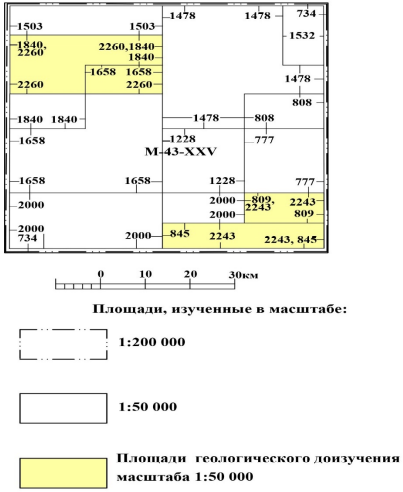
\includegraphics[width=5.37617in,height=3.52083in]{media/image16.png}

\textbf{Рис. 2 - Расположение водоема и села Кызылагаш}

На основе разработанной автоматизированной системы была выполнена модель
событий, произошедших 11- 12 марта 2010 года в селе Кызылагаш. По данным
Алматинского департамента по чрезвычайным ситуациям, авария произошла
вследствие сильного дождя и повышения температуры воздуха. Эти условия
привели к движению льда и спровоцировали образование селевых потоков.

Ситуация, развившаяся в селе Кызылагаш, была смоделирована с
использованием формулы (14) и представлена на рисунке 3.


\includegraphics[width=6.40001in,height=4.80001in]{media/image17.png}

\textbf{Рис. 3 - График максимальной волны прорыва в с.Кызылагаш}

Согласно данным на рисунке, волна прорыва, достигшая села Кызылагаш в
течение одного часа, имела высоту 1.5 метра. За этот же промежуток
времени высота волны, выходящей из водоема, снизилась с 12 метров до 7
метров.

Таким образом, результаты численного моделирования подтверждаются
фактическими данными, зафиксированными в ходе события.

\textbf{Выводы.} В рамках проведенного исследования достигнуты следующие
результаты:

\begin{itemize}
\item
  разработана математическая модель для прогнозирования последствий
  прорыва плотины. Создан алгоритм расчета максимального уровня волны
  прорыва, учитывающий различные параметры гидротехнического сооружения.
  Предложенный подход отличается высокой практической значимостью по
  сравнению с существующими методами;
\item
  на языке Python создан программно-аппаратный комплекс (ПАК) для
  мониторинга и прогнозирования последствий прорыва плотины;
\item
  на основе решения модельной задачи подтверждена эффективность
  разработанного ПАК. В качестве практической основы была использована
  ситуация, произошедшая в селе Кызылагаш Алматинской области Республики
  Казахстан;
\item
  полученные результаты могут быть использованы для поддержки принятия
  решений в органах управления водохозяйственной отрасли Казахстана.
  Предложенные методика и технологии обеспечивают качественно новый
  подход к задачам мониторинга водных ресурсов, выявлению явлений,
  способствующих чрезвычайным ситуациям, и оценке их последствий.
\end{itemize}

\emph{\textbf{Финансирование}. Работа выполнена за счет средств НИИ
математики и механики при КазНУ имени аль-Фараби и грантового
финансирования научных исследований на 2023--2025 годы по проекту
AP19678157.}

\textbf{Литература}

1.Хамутова М.В., Кушников В.А. Математическая модель прогнозирования
последствий наводнений//Вестник Астрахан. гос. техн. ун-та. Серия
управление, вычисл. техн. информ.- 2016.- № 3. - С. 109-114.

\begin{quote}
2.Симагин И.М., Полуян Л.В. Моделирование зон возможных затоплений при
авариях на гидротехнических сооружениях. SAFETY2018. -- Екатеринбург,
2018. -- С. 14-21. \url{http://elar.urfu.ru/handle/10995/66329ю} Дата
обращения:17.12.2024
\end{quote}

3.Стриганова М.Ю. Методы оценки и прогнозирование последствий при
разрушении гидротехнических сооружений // Вестник командно-инженерного
института МЧС Республики Белорусь.- 2012.- № 1(15). - С. 10-2.

4.Плеханов П.А. Гидрологические риски природного характера и их
предупреждение в Казахстане // Центрально-азиатский журнал исследований
воды. Специальный выпуск об опасностях, связанных с водой в Центральной
Азии. -- 2017. - № 3(1). - С. 19-25.

5.Молдабеков М.М., Еремир Д.И., Понятов Ю.А. Мониторинг уровня воды,
озер, рек морей и гидротехнических сооружений // Вестник КазНТУ.- 2013.
- №1. - С. 3-6.

6. Мазаков Т.Ж., Джомартова Ш.А., Мазакова А.Т., Шорманов Т.С., Алиаскар
М.С. Гибридная модель прогнозирования процесса селевого прорыва//Вестник
КазУТБ.-2024.- № 2(23). - С.1 20-126.
\href{https://doi.org/10.58805/kazutb.v.2.23-481}{DOI
10.58805/kazutb.v.2.23-481}

7.Мазаков Т.Ж., Джомартова Ш.А., Мазакова А.Т., Тойкенов Г.Ч., Алиаскар
М.С., Тойкенова У.Г. Идентификации математических моделей методом
квазилинераризации // Вестник КазУТБ. - 2024. - № 4(25).- C.16-23. DOI
10.58805/kazutb.v.4.25-650

8.Мазаков Т.Ж., Бургегулов А.Д., Джомартова Ш.А., Мазакова А.Т.,
Саметова А.А., Досаналиева А.Т. Построение маршрутов для эвакуации
сотрудников из здания при возникновении чрезвычайной ситуации // Вестник
КазУТБ. - 2024.- № 1(22).- C. 68-74

\href{https://doi.org/10.58805/kazutb.v.1.22-292}{DOI
10.58805/kazutb.v.1.22-292}

\textbf{References}

1.Hamutova M.V., Kushnikov V.A. Matematicheskaja model\textquotesingle{}
prognozirovanija posledstvij navodnenij//Vestnik Astrahan. gos. tehn.
un-ta. Serija upravlenie, vychisl. tehn. inform.- 2016.- № 3. - S.
109-114. {[}in Russian{]}

2.Simagin I.M., Polujan L.V. Modelirovanie zon vozmozhnyh zatoplenij pri
avarijah na gidrotehnicheskih sooruzhenijah. SAFETY2018. --
Ekaterinburg, 2018. -- S. 14-21.
http://elar.urfu.ru/handle/10995/66329ju Data
obrashhenija:17.12.2024{[}in Russian{]}

3.Striganova M.Ju. Metody ocenki i prognozirovanie posledstvij pri
razrushenii gidrotehnicheskih sooruzhenij // Vestnik
komandno-inzhenernogo instituta MChS Respubliki
Belorus\textquotesingle.- 2012.- № 1(15). - S. 10-2. {[}in Russian{]}

4.Plehanov P.A. Gidrologicheskie riski prirodnogo haraktera i ih
preduprezhdenie v Kazahstane // Central\textquotesingle no-aziatskij
zhurnal issledovanij vody. Special\textquotesingle nyj vypusk ob
opasnostjah, svjazannyh s vodoj v Central\textquotesingle noj Azii. --
2017. - № 3(1). - S. 19-25. {[}in Russian{]}

5.Moldabekov M.M., Eremir D.I., Ponjatov Ju.A. Monitoring urovnja vody,
ozer, rek morej i gidrotehnicheskih sooruzhenij // Vestnik KazNTU.-
2013. - №1. - S. 3-6. {[}in Russian{]}

6. Mazakov T.Zh., Dzhomartova Sh.A., Mazakova A.T., Shormanov T.S.,
Aliaskar M.S. Gibridnaja model\textquotesingle{} prognozirovanija
processa selevogo proryva//Vestnik KazUTB.-2024.- № 2(23). - S.1 20-126.
DOI 10.58805/kazutb.v.2.23-481{[}in Russian{]}

7.Mazakov T.Zh., Dzhomartova Sh.A., Mazakova A.T., Tojkenov G.Ch.,
Aliaskar M.S., Tojkenova U.G. Identifikacii matematicheskih modelej
metodom kvazilinerarizacii // Vestnik KazUTB. - 2024. - № 4(25).-
C.16-23. DOI 10.58805/kazutb.v.4.25-650{[}in Russian{]}

8.Mazakov T.Zh., Burgegulov A.D., Dzhomartova Sh.A., Mazakova A.T.,
Sametova A.A., Dosanalieva A.T. Postroenie marshrutov dlja jevakuacii
sotrudnikov iz zdanija pri vozniknovenii chrezvychajnoj situacii //
Vestnik KazUTB. - 2024.- № 1(22).- C. 68-74

DOI 10.58805/kazutb.v.1.22-292{[}in Russian{]}

\emph{\textbf{Сведения об авторах}}

Мазақова А.Т.- докторант КазНУ им.аль-Фараби, Алматы, Казахстан, e-mail:
\href{mailto:aigerym97@mail.ru}{\nolinkurl{aigerym97@mail.ru}}; ORCID:
https://orcid.org/\textbf{0000-0003-3019-3352}

Джомартова Ш.А. - доктор технических наук, доцент, КазНУ им. аль-Фараби,
Алматы, Казахстан, e-mail:
\href{mailto:jomartova@mail.ru}{\nolinkurl{jomartova@mail.ru}}; ORCID:
https://orcid.org/0000-0002-5882-5588

Мазақова Б.М. -- cт.преп. \emph{Казахский агротехнический}
исследовательский \emph{университет} имени С. Сейфуллина, Астана,
Казахстан, e-mail:
\href{mailto:bayan7080@mail.ru}{\nolinkurl{bayan7080@mail.ru}};
ORCID\textbf{:} https://orcid.org\textbf{/0000-0003-4904-3557}

Әлиасқар М.С. - старший преподаватель МИТУ, Алматы, Казахстан, e-mail:
\href{mailto:m.alyasqar@gmail.ru}{\nolinkurl{m.alyasqar@gmail.ru}};
ORCID:
https://orcid.org/\href{https://orcid.org/0000-0002-3013-6617}{0000-0002-3013-6617}

Мергенгали Е.К. -- докторант КазНУ имени аль-Фараби, Алматы, Казахстан,
e-mail:
\href{https://e.mail.ru/compose/?mailto=mailto\%3aestony.9999@gmail.com}{estony.9999@gmail.com};
ORCID:~https://orcid.org/0000-0002-9755-6472

Мазаков Т.Ж. - доктор физико-математических наук, профессор, КазНУ им.
аль-Фараби, Алматы, Казахстан, e-mail:
\href{mailto:tmazakov@mail.ru}{\nolinkurl{tmazakov@mail.ru}}; ORCID:
https://orcid.org/ 0000-0001-9345-5167

Досаналиева А.Т. - сеньор-лектор кафедры «Компьютерная инженерия»
Алматинского технологического Университета, Алматы, Казахстан, e-mail:
\href{mailto:Dosanalieva1985@gmail.com}{\nolinkurl{Dosanalieva1985@gmail.com}};
ORCID: \url{https://orcid.org/0009-0000-2958-1935}

Майлыбаева А.Д. -- к.ф.-м.н., доцент кафедры «Информатика» Атырауского
универститета имени Х. Досмухамедова, Атырау, Казахстан, e-mail:
\href{mailto:a.maylibayeva@asu.edu.kz}{\nolinkurl{a.maylibayeva@asu.edu.kz}};
ORCID: 0000-0003-0598-4806

\emph{\textbf{Information about the author}}

Mazakova A.T.- Doctoral student of Al-Farabi Kazakh National University,
Almaty, Kazakhstan, e-mail e-mail:
\href{mailto:aigerym97@mail.ru}{\nolinkurl{aigerym97@mail.ru}};

Jomartova Sh.A. - Doctor of Technical Sciences, Associate Professor,
Al-Farabi KazNU, Almaty, Kazakhstan, e-mail:
\href{mailto:jomartova@mail.ru}{\nolinkurl{jomartova@mail.ru}};

Mazakova B.M. - Senior Lecturer, Kazakh Agrotechnical Research
University named after S. Seifullin, Astana, Kazakhstan, e-mail:
\href{mailto:bayan7080@mail.ru}{\nolinkurl{bayan7080@mail.ru}};

Aliaskar M.S. - Senior Lecturer, MITU, Almaty, Kazakhstan, e-mail:
\href{mailto:m.alyasqar@gmail.ru}{\nolinkurl{m.alyasqar@gmail.ru}};

Mergengali E.K. - Doctoral student of Al-Farabi Kazakh National
University, Almaty, Kazakhstan, e-mail:
\href{mailto:estony.9999@gmail.com}{\nolinkurl{estony.9999@gmail.com}};

Mazakov T.Zh. - Doctor of Physical and Mathematical Sciences, Professor,
Al-Farabi KazNU, Almaty, Kazakhstan, e-mail:
\href{mailto:tmazakov@mail.ru}{\nolinkurl{tmazakov@mail.ru}};

Dosanalieva A.T. - Senor Lecturer, Computer Engineering Department,
Almaty Technological University, Almaty, Kazakhstan, e-mail:
\href{mailto:Dosanalieva1985@gmail.com}{\nolinkurl{Dosanalieva1985@gmail.com}}

Mailybayeva A.D. - PhD, Associate Professor, Department of Computer
Science, Atyrau University named after Kh. Dosmukhambetov, Atyrau,
Kazakhstan, e-mail:
\href{mailto:a.maylibayeva@asu.edu.kz}{\nolinkurl{a.maylibayeva@asu.edu.kz}};
ORCID: https://orcid.org/0000-0003-0598-4806

МРНТИ 28.23.17

\textbf{КЛАССИФИКАЦИЯЛЫҚ АЛГОРИТМДЕРДІ ҚОЛДАНЫП ДАУЫСТЫ ТАНУ}

\textbf{\textsuperscript{1}Н.О.Мекебаев}

\includegraphics[width=0.14583in,height=0.14583in]{media/image1.png}\textbf{\textsuperscript{🖂},
\textsuperscript{2}Д.К.Даркенбаев}
\includegraphics[width=0.14583in,height=0.14583in]{media/image1.png}
\textbf{, \textsuperscript{1}Н.А. Модовов}

\includegraphics[width=0.14583in,height=0.14583in]{media/image1.png}\textbf{,
\textsuperscript{1}Ж.А.
Орынтаева}
\includegraphics[width=0.14583in,height=0.14583in]{media/image1.png}

\textsuperscript{1}Қазақ ұлттық қыздар педагогикалық университеті,
Алматы, Қазақстан

\textsuperscript{2}Әл-Фараби атындағы Қазақ ұлттық университеті, Алматы,
Қазақстан

\textbf{\textsuperscript{🖂}}Корреспондент-автор:
\ul{\href{mailto:nurbapa@gmail.com}{\nolinkurl{nurbapa@gmail.com}}}

Дауыс тану жүйелері машиналық оқыту әдістеріне негізделген, оның ішінде
классификациялық алгоритмдер кеңінен қолданылады. Классификация дауыс
сигналдарын әртүрлі санаттарға, мысалы, сөздер немесе сөйлемдерге бөліп
тануды жүзеге асырады. Бұл үдерісте жиі қолданылатын алгоритмдерге
логистикалық регрессия, шешім ағаштары және нейрондық желілер жатады.
Дауыс сигналын өңдеуде алдымен ерекшеліктері, яғни маңызды параметрлері,
экстракцияланады, содан кейін олар классификаторға беріледі.
Классификация нәтижесінде жүйе сөйлеген сөзді мәтінге түрлендіреді
немесе дыбыстың нақты мазмұнын анықтайды. Бұл технология адам-компьютер
өзара әрекеттестігін жақсарту үшін маңызды. Бұл мақалада машиналық оқыту
әдістерін қолдана отырып, сөйлеушінің даусын анықтау мәселесін шешу үшін
жіктеу алгоритмдерін қарастырамыз. Сөйлеудің алдын ала өңдеуде МҒСС-ті
алгортимін пайдаландық. Жоғарыдағы мәселені шешу үшін бес жіктеу
алгортмі қарастырылып, салыстырмалы талдау жасалды. Алғашқы эксперимент
жасағанда ең жақсы нәтиже көрсеткен SVC алгортимі 0,90 және MLP
Classifier алгоритмі 0,83 нәтижелерін көрсетті. Келесі экспермиентте
жеке тұлғаның дауысын анықтауда неғұрлым үлкен дәлдікте Robust scaler
әдісімен масштабтауда -- 0,93 көпқабатты персептрон көрсете бастады.
Сондықтан бұл мәселені шешу үшін сөйлеу сигналының ерекшелігін ескеретін
көп қабатты перцептронды қолдануға болады.

\textbf{Түйін сөздер:} алгортим, дауыс, сөйлеуді тану, ASR, MFCC, MLP.

\textbf{РАСПОЗНАВАНИЕ ГОЛОСА С ПОМОЩЬЮ АЛГОРИТМОВ КЛАССИФИКАЦИИ}

\textbf{\textsuperscript{🖂 1}Н.О.Мекебаев,
\textsuperscript{2}Д.К.Даркенбаев, \textsuperscript{1}Модовов Н.А,
\textsuperscript{1}Орынтаева Ж.А.}

\textsuperscript{1}Казахский национальный женский педагогический
университет, Алматы, Казахстан

\textsuperscript{2}Казахский национальный университет им. Аль-Фараби,
Алматы, Казахстан

e-mail:
\ul{\href{mailto:nurbapa@gmail.com}{\nolinkurl{nurbapa@gmail.com}}}

Системы распознавания речи основаны на методах машинного обучения, среди
которых широко применяются классификационные алгоритмы. Классификация
выполняет задачу разделения голосовых сигналов на различные категории,
такие как слова или предложения. К часто используемым алгоритмам
относятся логистическая регрессия, деревья решений и нейронные сети. В
процессе обработки голосового сигнала сначала извлекаются его
особенности, то есть важные параметры, которые затем передаются
классификатору. По результатам классификации система преобразует речь в
текст или определяет конкретное содержание звука. Эта технология важна
для улучшения взаимодействия человека с компьютером. В данной статье
обсуждается алгоритм классификации для задачи идентификации речи с
использованием метода машинного обучения. Алгоритм MFCC используется для
предварительной обработки речи. Для решения этой задачи проведен
сравнительный анализ пяти алгоритмов классификации. В первом
эксперименте были определены методы опорного вектора -- 0,90 и
многослойного перцептрона -- 0,83 и показаны лучшие результаты. Во
втором эксперименте был предложен многослойный перцептрон с точностью
0,93 с использованием метода Робастного скалера для идентификации
личности. Поэтому для решения этой проблемы можно использовать
многослойный персептрон, учитывающий детали аудиосигнала.

\textbf{Ключевые слова:} алгортим, голос, распознавание речи, ASR, MFCC,
MLP.

\textbf{VOICE RECOGNITION USING CLASSIFICATION ALGORITHMS}

\textbf{\textsuperscript{🖂1}N.Mekebayev,
\textsuperscript{2}D.Darkenbayev, \textsuperscript{1}N.Modovov,
\textsuperscript{1}Zh.Oryntaeva.}

\hl{\textsuperscript{1}}Kazakh National Women\textquotesingle s
Pedagogical University, Almaty, Kazakhstan

\textsuperscript{2}Al-Farabi Kazakh National University, Almaty,
Kazakhstan

e-mail:
\ul{\href{mailto:nurbapa@gmail.com}{\nolinkurl{nurbapa@gmail.com}}}

In Speech recognition systems are based on machine learning methods,
among which classification algorithms are widely used. Classification
performs the task of dividing voice signals into various categories,
such as words or sentences. Commonly used algorithms include logistic
regression, decision trees, and neural networks. During voice signal
processing, features, i.e., important parameters, are first extracted
and then passed to the classifier. Based on the classification results,
the system converts speech into text or determines the specific content
of the sound. This technology is essential for improving human-computer
interaction.This article discusses a classification algorithm for the
problem of speech identification using the machine learning method. The
MFCC algorithm is used for preprocessing speech. To solve this problem,
a comparative analysis of five classification algorithms was carried
out. In the first experiment, the methods of the reference vector --
0.90 and the multilayer perceptron -- 0.83 were determined and the best
results were shown. In the second experiment, a multilayer perceptron
with an accuracy of 0.93 was proposed using the Robust Scaler method for
personality identification. Therefore, a multilayer perceptron can be
used to solve this problem, taking into account the details of the audio
signal. be used, taking into accaudio. s.

\textbf{Keywords:} algorithm, voice, speech recognition, ASR, MFCC, MLP.

\textbf{Кіріспе.} Ауыз екі сөйлеу тілін тану -- аудиодағы сөйлеуші
сөйлейтін тілді жіктеу мәселесі. Ол әдетте сөздің тілдік санатын
бастапқыда анықтау үшін, кейіннен өңдеуді жеңілдету үшін көптілді
автоматты сөйлеуді тану (ASR) сияқты көптілді сөйлеуді өңдеу
тапсырмаларының алдыңғы бөлігі ретінде пайдаланылады. Тұрақты және
сенімді тілді сәйкестендіру жүйесі бұл жүйелерде жоғары өнімділік пен
дәлдікке жетудің кілті болып табылады {[}1{]}.

Зерттеудің мақсаты сөйлеушінің дауысын анықтауға арналған машиналық
оқытудың классификациялық әдістерін зерттеу. Осы мақсатқа жету үшін
келесі міндеттер орындалды. Классификация алгоритміне салыстырмалы
талдау жүргізіліп бірқатар жіктеу алгоритмдері және сөйлеуді алдын ала
өңдеу мәселелері қарастырылды {[}2{]}.

Дәстүрлі тілдік анықтау көбінесе акустикалық және фонетикалық
ерекшеліктерге сүйенеді. Жалпы акустикалық сипаттамаларға, басқалармен
қатар, кепстральды мель-жиілік коэффициенттері (MFCC), дельта
коэффициенттері, перцептивті сызықтық болжау коэффициенттері (PLP) және
кепстральды гамма-жиілік коэффициенттері жатады {[}3{]} .

Соңғы жылдары cөйлеуді автоматты түрде тану (ASR), визуалды сөйлеуді
тану ((VST) және аудиовизуалды сөйлеуді тану (AVSR) салаларында ауқымды
ғылыми-зерттеу жұмыстары жүргізілуде {[}4{]}.

Бұл мақалада дауысты (сөйлеу екі тілді) тануды қарастырамыз. Тілді тану
-- бұл сөйлеушіні тануға ұқсас мәселе, өйткені біз белгілі бір сөздің
мазмұны туралы емес, бүкіл мәлімдеме туралы ақпарат алуға тырысамыз.
Жіктеу алгортимдері техникасындағы дауысты (тілді) тануға қолдану біздің
әдістеріміздің жан-жақты екенін және сөйлеудің бірнеше саласында
әлеуетті қолданылатынын көрсетеді {[}5{]}.

Қазақстанда қазақ тілінің сөйлеу технологиялары зерттелуде. Қазақ тілі
агглютинативті тілдер тобына жатады. Агглютинативті тілдердің
құрылымында әр түрлі форматтағы қосымшалар (жұрнақтар, жалғаулар)
бірінен соң бірі кезектесіп қосылады, бұл сөзді өзгертудің басым түрі
болып табылады және осы қосымшалардың әрқайсысы тек бір мағынамен
жүктеледі {[}6{]}. Түрік, моңғол, корей тілдері агглютинативті тілдерге
жатады. Біздің елімізде қазақ тіліндегі тұлғаны тану жүйесі әлі
дамымаған, бұл аталған бағыттағы зерттеулерді өзекті етеді.

Бұл мақалада жіктеу алгоритмдерін қолдана отырып, дауысты тану, анықтау
міндеттерін қарастырамыз.

\textbf{\hl{Материалдар мен әдістер.}} Сөйлеуді тану үдерісі негізінде
алдын ала өңдеуден тұрады {[}7{]}. Осы мақалада біз дауыстың динамикалық
өңдеуде МҒСС-ті қолданамыз. Сөйлеу сигналының алдын-ала өңдеу үдерісі
1-ші суретте көрсетілген. MFCC (Mel-Frequency Cepstral Coefficients) мел
жиілігінің кепстральды коэффициенттері дауыс, дыбыспен жұмыс жасау
кезінде ең танымал таңдау болып табылады. Бұл тәсілдің ерекшелігі -
бастапқы сигналдың ұзындығынан алынған сипаттамалар векторы және ондағы
сөйлейтін жеке ерекшеліктердің таралуын есепке алу {[}8{]}.

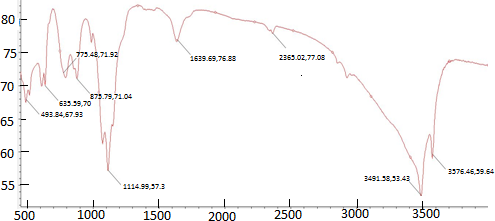
\includegraphics[width=5.8604in,height=2.31982in]{media/image18.png}

\textbf{1-- сурет. Сөйлеу сигналын алдын ала өңдеу}

Әрбір жазылған аудио негізінде 5806 белгі алынды. Аудио файлдағы әрбір
кез-келген дауыс жазылып жатқан сигнал динамиктің белгі атымен
белгіленеді. Осы алынған дерек, мәліметтер жиынының жалпы өлшемі
1285x5806.

Кепстр -- бұл сүзгіні дыбыс толқынының көзінен бөлетін түрлендіру.

Көрсетілгенді визуализациялау үшін 5806 белгісі бар векторлық
кеңістіктің және екі-үш өлшемді кеңістіктің өлшемдерін азайту үшін
негізгі компоненттер әдісі қолданылады. Дисперсияны негізгі компонент
әдісімен кішірейтілген мөлшерде сақтау 2-суретте көрсетілген.

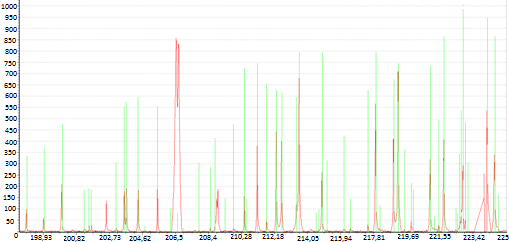
\includegraphics[width=4.45544in,height=2.42321in]{media/image19.png}

\textbf{2 - сурет. Негізгі құрамдас әдісті пайдаланып өлшемділікті
азайту кезінде дисперсияны сақтау}

Жоғарыда келтірілген графикте көрсетілгендей, деректердің өлшемі 1285
белгіге дейін төмендеген жағдайда дисперсия 98,9 \% сақталады. Алайда,
жіктеу модельдерімен және деректер стандарттаушыларымен жүргізілген
тәжірибе көрсеткендей, бұл кішірейту конструктивті түрде жіктеудің
дәлдігіне ықпал етеді.

\textbf{Материалдар мен әдістер.} Эксперимент жасау үшін деректерді
«Ақпараттық және есептеуіш технологиялар» инситутының зерттеушілерінің
базасынан алынды {[}9{]}. Берілген деректер, мәліметтер жиынтығы 0-19
сөйлеушінің 1285 аудио жазбасынан тұрды, олардың әрқайсысы 68-76
сөйлемнен тұратын жазбаны жазды. Қазақ тіліндегі әрбір аудиожазба орта
есеппен 5 секундқа созылатын сөз тіркесін білдіреді. Сөйлеушіні тану
үшін біз келесі деректер, мәліметтерді жинадық: сөйлеушінің аты,
сөйлеушінің жынысы, сөйлеушінің туған жері, сөйлеушінің туған жылы.
Төмендегі 1 кестеде сөйлеушінің мәліметтері көрсетілген.

\textbf{1 -- кесте. Сөйлеушінің мәліметтері}

\begin{longtable}[]{@{}
  >{\raggedright\arraybackslash}p{(\columnwidth - 12\tabcolsep) * \real{0.0943}}
  >{\raggedright\arraybackslash}p{(\columnwidth - 12\tabcolsep) * \real{0.1578}}
  >{\raggedright\arraybackslash}p{(\columnwidth - 12\tabcolsep) * \real{0.1068}}
  >{\raggedright\arraybackslash}p{(\columnwidth - 12\tabcolsep) * \real{0.1961}}
  >{\raggedright\arraybackslash}p{(\columnwidth - 12\tabcolsep) * \real{0.1237}}
  >{\raggedright\arraybackslash}p{(\columnwidth - 12\tabcolsep) * \real{0.1540}}
  >{\raggedright\arraybackslash}p{(\columnwidth - 12\tabcolsep) * \real{0.1673}}@{}}
\toprule\noalign{}
\begin{minipage}[b]{\linewidth}\raggedright
ТАӘ
\end{minipage} & \begin{minipage}[b]{\linewidth}\raggedright
Тегі
\end{minipage} & \begin{minipage}[b]{\linewidth}\raggedright
Аты
\end{minipage} & \begin{minipage}[b]{\linewidth}\raggedright
Әкесінің аты
\end{minipage} & \begin{minipage}[b]{\linewidth}\raggedright
Жынысы
\end{minipage} & \begin{minipage}[b]{\linewidth}\raggedright
Туған жері
\end{minipage} & \begin{minipage}[b]{\linewidth}\raggedright
Туған жылы
\end{minipage} \\
\begin{minipage}[b]{\linewidth}\raggedright
МЖА
\end{minipage} & \begin{minipage}[b]{\linewidth}\raggedright
Масимканова
\end{minipage} & \begin{minipage}[b]{\linewidth}\raggedright
Жазира
\end{minipage} & \begin{minipage}[b]{\linewidth}\raggedright
Ауезбеккызы
\end{minipage} & \begin{minipage}[b]{\linewidth}\raggedright
әйел
\end{minipage} & \begin{minipage}[b]{\linewidth}\raggedright
Алматы
\end{minipage} & \begin{minipage}[b]{\linewidth}\raggedright
20.03.1982
\end{minipage} \\
\begin{minipage}[b]{\linewidth}\raggedright
ИМТ
\end{minipage} & \begin{minipage}[b]{\linewidth}\raggedright
Искакова
\end{minipage} & \begin{minipage}[b]{\linewidth}\raggedright
Молдир
\end{minipage} & \begin{minipage}[b]{\linewidth}\raggedright
Тасболаткызы
\end{minipage} & \begin{minipage}[b]{\linewidth}\raggedright
әйел
\end{minipage} & \begin{minipage}[b]{\linewidth}\raggedright
Алматы
\end{minipage} & \begin{minipage}[b]{\linewidth}\raggedright
01.01.1994
\end{minipage} \\
\begin{minipage}[b]{\linewidth}\raggedright
ДАЖ
\end{minipage} & \begin{minipage}[b]{\linewidth}\raggedright
Дүйсенбаева
\end{minipage} & \begin{minipage}[b]{\linewidth}\raggedright
Айгерім
\end{minipage} & \begin{minipage}[b]{\linewidth}\raggedright
Жанболаткызы
\end{minipage} & \begin{minipage}[b]{\linewidth}\raggedright
әйел
\end{minipage} & \begin{minipage}[b]{\linewidth}\raggedright
Алматы
\end{minipage} & \begin{minipage}[b]{\linewidth}\raggedright
15.05.1995
\end{minipage} \\
\begin{minipage}[b]{\linewidth}\raggedright
ЖЕА
\end{minipage} & \begin{minipage}[b]{\linewidth}\raggedright
Жетписбаев
\end{minipage} & \begin{minipage}[b]{\linewidth}\raggedright
Ерлан
\end{minipage} & \begin{minipage}[b]{\linewidth}\raggedright
Алибекович
\end{minipage} & \begin{minipage}[b]{\linewidth}\raggedright
ер
\end{minipage} & \begin{minipage}[b]{\linewidth}\raggedright
Алматы
\end{minipage} & \begin{minipage}[b]{\linewidth}\raggedright
23.05.1995
\end{minipage} \\
\begin{minipage}[b]{\linewidth}\raggedright
ССМ
\end{minipage} & \begin{minipage}[b]{\linewidth}\raggedright
Самрат
\end{minipage} & \begin{minipage}[b]{\linewidth}\raggedright
Санжар
\end{minipage} & \begin{minipage}[b]{\linewidth}\raggedright
Мұхаметқалиулы
\end{minipage} & \begin{minipage}[b]{\linewidth}\raggedright
ер
\end{minipage} & \begin{minipage}[b]{\linewidth}\raggedright
Алматы
\end{minipage} & \begin{minipage}[b]{\linewidth}\raggedright
12.07.1996
\end{minipage} \\
\midrule\noalign{}
\endhead
\bottomrule\noalign{}
\endlastfoot
\end{longtable}

\emph{Жіктеу алгоритмдері}

Сөйлеушіні анықтау тану мәселесін шешуде төмендегідей жіктеу
алгоритмдерін қарастырдық:

\emph{MLP Classifier алгоритмі}

MLP көп қабатты перцептрон -
\((Y) = T_{n}:{\ \ T}_{n} \rightarrow T^{0}\) функциясын аудио деректер
сериясында оқыту арқылы зерттейтін басқарылатын оқыту алгоритмі, мұндағы
n - енгізу үшін өлшемдер саны, а\textsubscript{0}-шығару үшін өлшемдер
саны. \(Y = y_{1},y_{2},\ldots,y_{n}\) функцияларының жиынтығын ескере
отырып ` \(y_{n}\)' ол кез-келген классификация үшін сызықтық емес
функциялардың жуықтауын зерттей алады. 3-ші суретте MLP архитектурасы
көрсетілген.

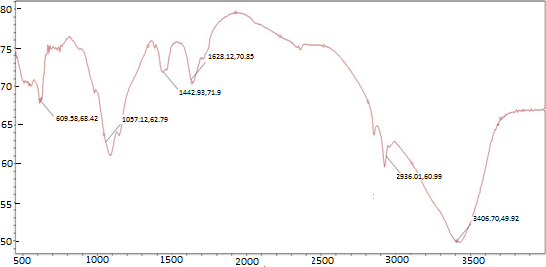
\includegraphics[width=3.94724in,height=2.64584in]{media/image20.png}

\textbf{\hl{3}} -- \textbf{\hl{сурет}}. \textbf{\hl{MLP архитектурасы}}

Кіріс қабаты кіріс функцияларын білдіретін
\hl{}\(x_{1},\ x_{2},\ ...,x_{n\ }\ \)тұрады. Шығыс қабаты соңғы жасырын
қабаттан мәндерді алады және оларды шығару мәндеріне түрлендіреді.

\emph{Extra-Trees алгортимі}

Extra-Trees алгоритмі жаңартылмайтын шешімдер немесе регрессиялар
ансамблін жасайды. Қадамға негізделген ансамбльдің басқа әдістері
алгоритмнің екі негізгі айырмашылығы-ол кездейсоқ түрде кесу нүктелерін
таңдап, түйіндерді сындырады және қадамдарды ұлғайту үшін бүкіл оқу
үлгісін пайдаланады {[}10{]}.

\emph{Trees\_node(M)}

Тұрақты оқыту жиынтығы N түйініне сәйкес келіп кіріс синалын айналады.

шығыс синалы ретінде {[}\(d\) \textless{} \(d_{c}\){]} аламыз

-- оқытуда \emph{Tree(S.)} ақиқат болған жаңдайда ешнәрсе қайтарылмайды

-- ондай жағдайда тұрақты емес барлық (S) атрибуттарының топтарының
ішіндегі \{\(d_{1}\),...\({,d}_{K}\)\} атрибуттарын тұрақты түрде
таңдаймыз;

-- осы K қадамдарды \{g\textsubscript{1},...,g\textsubscript{K} \}
таңдап, мұндағы g\textsubscript{i} = \emph{Random\_split.}(G,
d\textsubscript{i}), ∀ i = 1,..., K.;

--g\textsubscript{∗} сегменттерінде Score(g\textsubscript{∗}, G.) =
max\textsubscript{i=1,...,K} Score(g\textsubscript{i}, G.) деп
келтіреміз.

\emph{Random\_split.(S,} \(a\)\emph{)}

G ішкі жиыны және d атрибуты кірісі.

-- \(d_{\max}^{G}\) және \(d_{\min}^{G}\) минималды мәнді, максималды
мәнін G-ге біріктіреді;

\emph{Tree(S.)}

G ішкі жиынның кірісі

\(d\) логикалық мәні шығысы

-- егерде \textbar{} G \textbar{} \textless{} n\textsubscript{min} болса
қайтару ақиқатты көрсетеді;

-- егер барлық G атрибуттары тұрақты болса, біз TRUE (ақиқат)мәнін
қайтарамыз;

-- егер G шығысы тұрақты болса, біз true (ақиқат)қайтарамыз;

-- болмаған жағдайда біз false (жалған) мәнін қайтарамыз.

Оның екі параметрі бар: K әр түйін үшін кездейсоқ таңдалған атрибуттар
саны және n\textsubscript{min} түйінді бөлу үшін ең кіші үлгінің өлшемі.
Ол ансамбль моделін құру үшін бастапқы оқыту моделімен бірнеше рет
қолданылады {[}11{]}.

\emph{SVC алгоритмі}

Сызықтық бөлінетін екілік жіктеу мәселесін шешу үшін SVC пайдалану үшін
бізге қажет:

\begin{itemize}
\item
  \emph{J-}ді құруда\textbf{,} мұндағы
  \(J_{ij} = z_{i}z_{j}y_{i} \bullet y_{j}\)
\item
  σ --ны табу;
\item
  \(\sum_{i = 1}^{M}{}{\sigma\ }_{i} - \frac{1}{2}{\sigma\ }^{T}J\sigma\ \)
\item
  \({\sigma\ }_{i} \geq 0\ \ \ \ \ \ \forall_{i}\ және\ \sum_{i = 1}^{M}{}{\sigma\ }_{i}z_{i} = 0\ \)осы
  шектеу аймақтарын ескере қарап, мейілінше жоғарылату;
\item
  QN шешімді қолдану болып табылады;
\item
  \(v = \sum_{i = 1}^{M}{}{\sigma\ }_{i}z_{i}y_{i}\) есептеу;
\item
  \({\sigma\ }_{i} > 0\ \ \ \ \ \ \)индекстерін есептеп, \emph{l} тірек
  әрбір векторының санын анықтау;
\item
  \(a = \frac{1}{M_{s}}\sum_{l \in L}^{}{}({\sigma\ }_{m}z_{m}y_{m} \bullet y_{L}\)
  есептеу керек;
\item
  \(y^{'}\ \)кез-келген нүктесі \(z^{'} = sgn(v \bullet y^{'} + a\)
  есептеу тәсілімен жіктеуге болады.
\end{itemize}

\emph{Gaussian NB алгоритмі}

Осы Naive Bayes - \(y_{1},\ y_{2},\ ...,y_{n\ }\) тізбегіндегі
көбейтіндісіне с пропорционал \(А_{k}\)класының ішінде жататын
\(m + 1\ \)деректер нүктесінің нақты ықтималдығын береді. \(m\)
алдыңғы\(\ \sigma\left( A_{k} \right) -\)класы мен
\(\sigma\left( А_{a} \right)\prod_{i = 1}^{m}{}\sigma\left( A_{k} \right)\ \)белгілерінің
арасындағы шартты ықтималдығы болып табылады {[}12{]}.

\(\sigma(A_{a}\))\(\prod_{i = 1}^{m}{}\sigma\left( A_{a} \right) > \sigma(A_{b})\prod_{i = 1}^{m}{}\sigma(y_{i}|A_{b})\)

\[\sigma\left( y_{1},\ldots,y_{n} \right) > \sigma(A_{b}|y_{1},\ldots,\ y_{n})\]

Осылайша, \(y_{1},\ y_{2},\ ...,y_{n\ }\ \) мәліметтер нүктесіне кластың
осы ең ықтимал нақты тағайындалуы \(а = 1,\ldots,А\) үшін
\(\sigma\left( А_{a} \right)\prod_{i = 1}^{m}{}\ \sigma\left( A_{k} \right)\ \)есептеудің
мәні макисмум болып табылатын \(А_{k}\ \)класындағы
\(y_{1},\ y_{2},\ ...,y_{n\ }\ \)есептеу ықтималдығы.

\emph{KNN алгоритмі}

KNN алгоритмі сұрау көрінісі мен мәліметтер жиынтығындағы көрініс
жиынтығы арасындағы ара қашықтықты өлшейді.

Тестілеу модельдеу нысандарының әрқайсысын жіктеу үшін келесі
әрекеттерді жүйелі түрде орындау қажет:

- оқыту моделінің әрбір нысанына дейінгі ара қашықтықты есептеу керек;

- K-ны оқыту моделінің нысанын таңдау керек;

- К классификацияланған объектінің класы жақын көршілер арасында ең көп
таралған класс болып табылады.

Жоғарыдағы ұсынылған алгоритмдер тұлғаны сәйкестендіру, сөйлеушіні тану
мәселесіне қолданылып, салыстырмалы талдау жүргізілді. Салыстырмалы.
талдаулар мен эксперименттер олардың ең жақсы екенін көрсетеді.
Нәтижелерінде тірек векторлық машиналар мен көп қабатты перцептронды
қолдану арқылы алынды. 4-ші суретте осы мәліметтер жиынының жіктеу
дәлдігі көрсетілген.

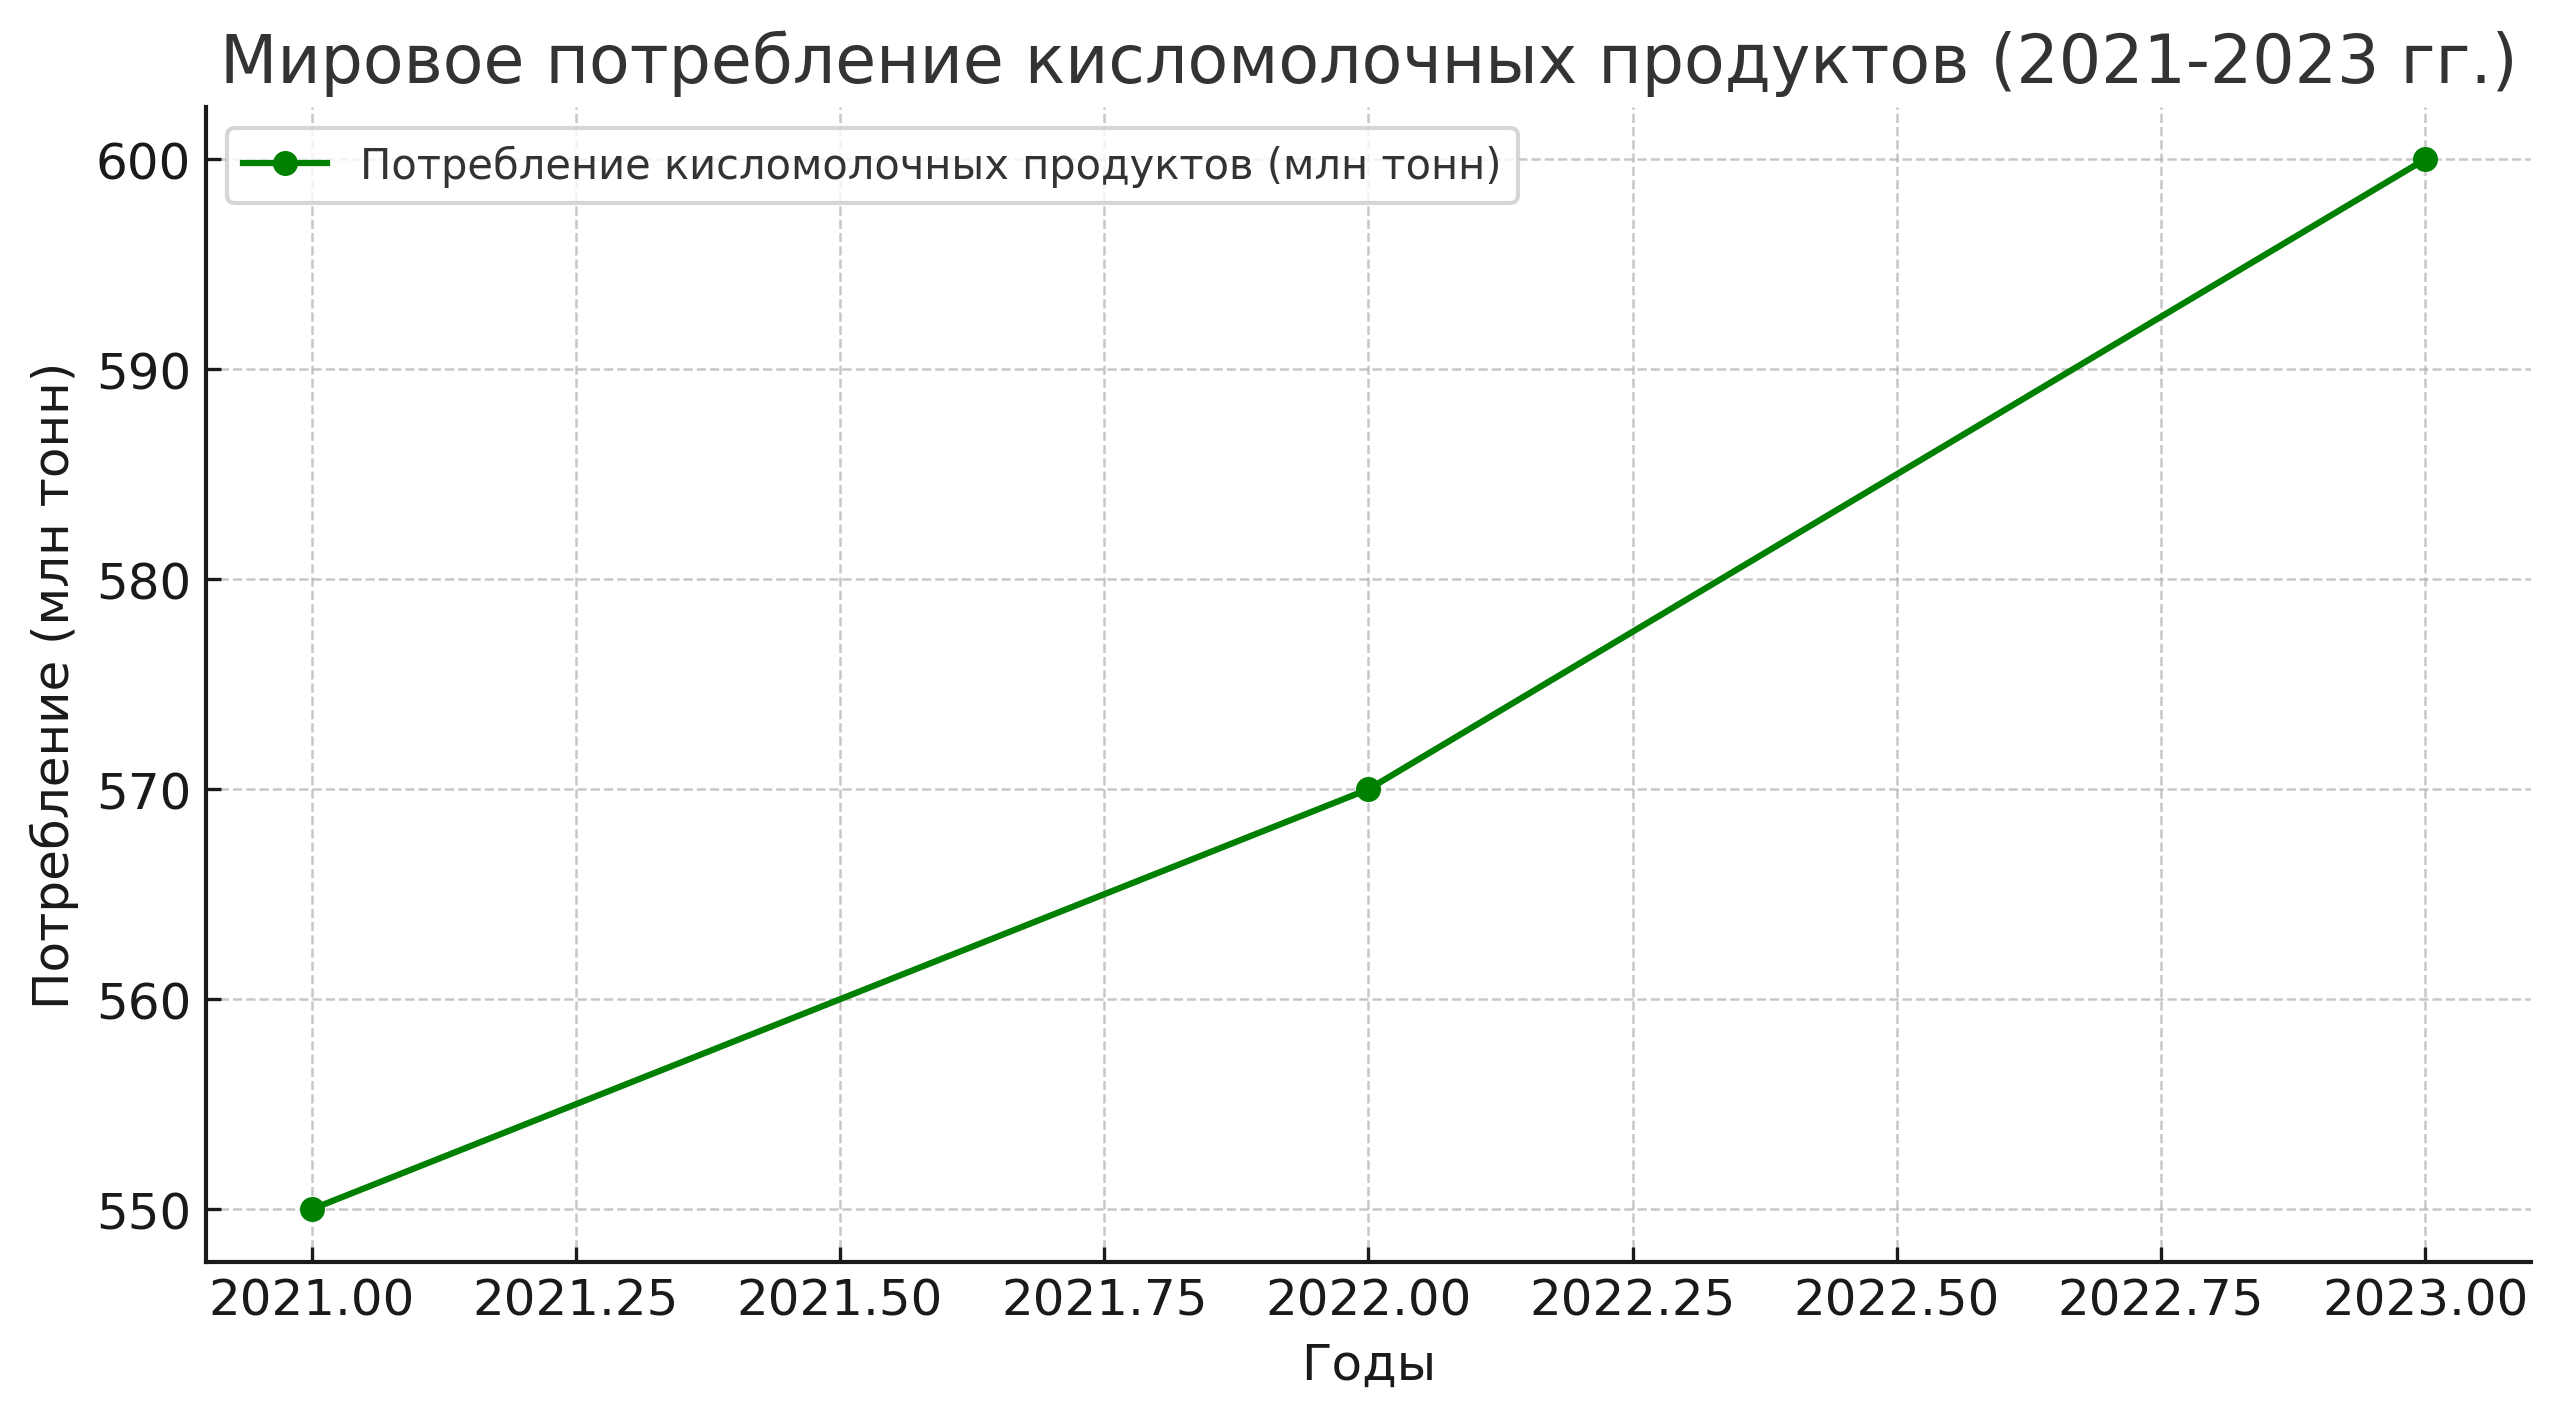
\includegraphics[width=5.40233in,height=2.24342in]{media/image21.png}

\textbf{4 -- сурет. Деректер жиынының жітеу дәлдігі}

4-ші суреттен көрініп тұрғандай тірек векторлық машина мен көпқабатты
перцептрон ең жақсы нәтиже көрсетті -- сәйкесінше 0,90 және 0,83.

Нәтижелерді жақсарту үшін біз әртүрлі әдістерді қолданып масштабтау
жасап, нәтижелердің өзгергені байқалды. 5 -- суретте әртүрлі әдістерді
қолдану арқылы деректерді масштабтау кезіндегі жіктеу дәлдігі
көрсетілген.

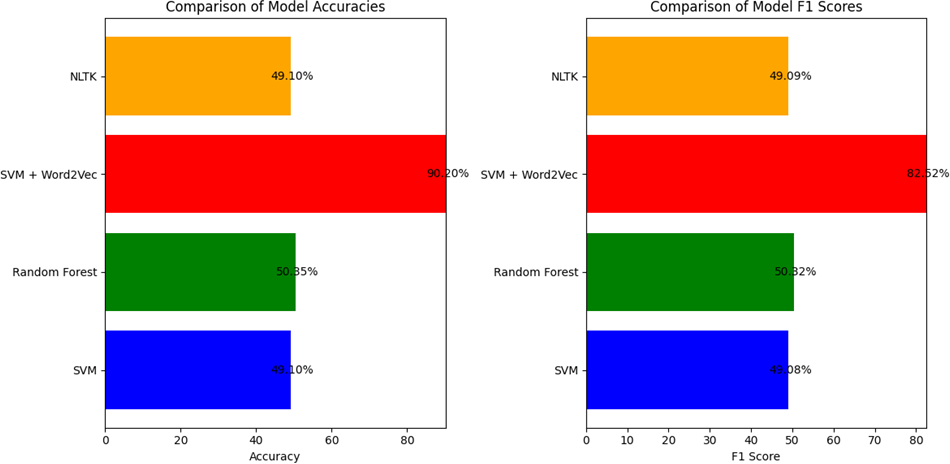
\includegraphics[width=5.72927in,height=2.5021in]{media/image22.png}

\textbf{5 -- сурет. Әртүрлі әдістерді қолдану арқылы деректерді
масштабтау кезіндегі жіктеу дәлдігі}

Көпқабатты перцептрон сенімді Robust scaler әдісін қолданып масштабтаған
кезде ең жоғары дәлдікке 0,93 жетті, ал тірек векторлық машиналар
дәлдігі азая бастады, бірақ Standard scaler және MaxAb Scaler әдісімен
масштабтау кезінде дәлдік нәтижелері 0,90-нан 0,91-ге дейін жақсарды.

Сөйлеу нысандарының өлшемділігін 1390-ға дейін азайту үшін негізгі
құрамдас талдауды пайдалансаңыз, жіктеу дәлдігі 2-кестеде көрсетілгендей
өзгереді.

\textbf{2 - кесте. Өлшемді азайту арқылы деректер бойынша жіктеу
дәлдігі}

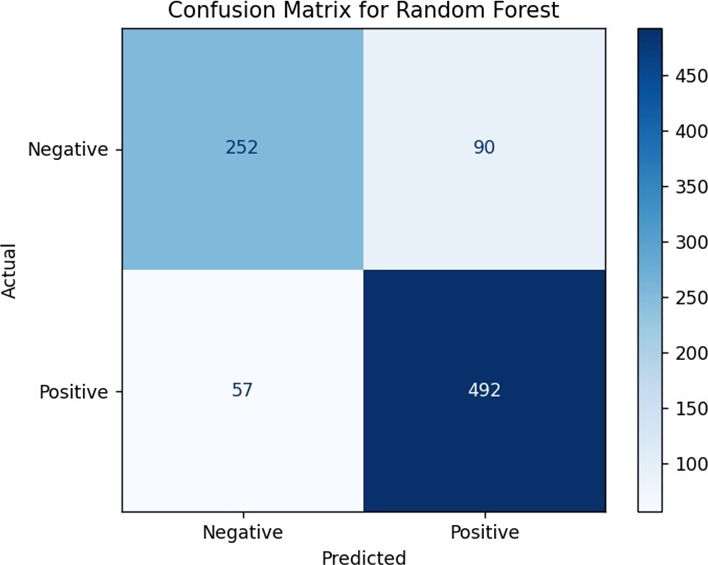
\includegraphics[width=5.94532in,height=1.86914in]{media/image23.png}

Салыстырмалы талдаудың мақсаты жеке сөйлеушіні тану мәселесіне жіктеу
алгоритмінің әсер ету дәрежесін анықтау, сонымен қатар SVC және MLP
жіктеуіш алгоритмдерін салыстырмалы бағалау болды. Дауыс деректерінің
үлгілерін оқыту бойынша жүргізілген эксперименттер осы алгоритмдердің
келешегі туралы айтуға мүмкіндік беретін нәтижелерді көрсетеді. Алынған
мәліметтер 6 және 7-суреттерде берілген.

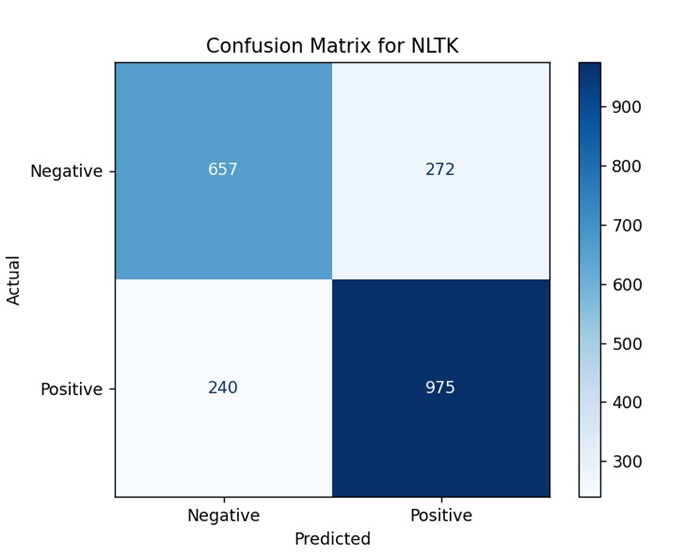
\includegraphics[width=4.02096in,height=2.99073in]{media/image24.png}

\textbf{6 -- сурет. Дыбыстық деректердің, сөйлеу белгілерінің үш өлшемді
көрінісі}

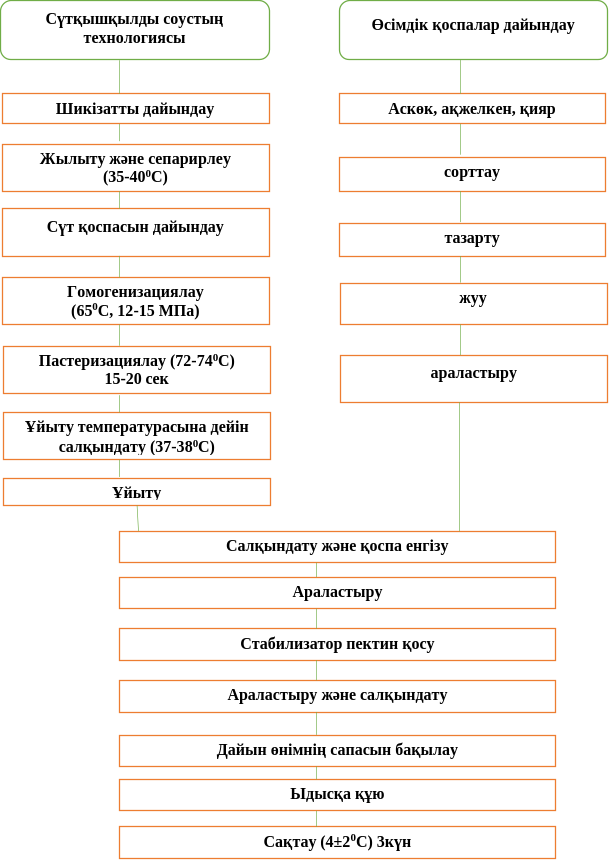
\includegraphics[width=4.97822in,height=2.75975in]{media/image25.png}

\textbf{7 -- сурет. Дыбыстық деректердің, сөйлеу белгілерінің екі
өлшемді көрінісі}

Әртүрлі әдістерді қолдану арқылы деректерді, масштабтау кезіндегі жіктеу
нәтижелері алдын ала экспериментте алынған нәтижелерден айтарлықтай
ерекшеленетіні анықталды.

\textbf{Қортынды.} Бұл мақалада біз бірнеше жіктеу алгоритмдерін және
сөйлеуді алдын ала өңдеу мәселесін қарастырдық. Тәжірибе нәтижелерін
талдау негізінде Robust scaler әдісімен масштабтау үшін дәлдігі 0,93
көпқабатты перцептрон ұсынылады, ал сөйлеу сигналын көпқабатты
перцептрон көмегімен жіктеуге болатындығы анықталды. Содан кейін алынған
деректерге сүйене отырып, сөйлеушіні тану үдерісін анықтадық.

Әрі қарайғы зерттеу барысында біз алынған мәліметтердің шынайылығын
тексеру мәселесін шешеміз деп үміттенеміз.

\textbf{Әдебиеттер}

\begin{enumerate}
\def\labelenumi{\arabic{enumi}.}
\item
  Matejka, P.; Zhang, L.; Ng, T.; Glembek, O.; Ma, J.; Zhang, B.;
  Mallidi, S.H. Neural Network Bottleneck Features for Language
  Identification // In Proceedings of the Speaker and Language
  Recognition Workshop (Odyssey 2014). - Joensuu, Finland, 16--19 June
  2014. -P. 299--304. DOI: 10.21437/Odyssey.2014-45
\item
  Pliakos K., Geurts P., Vens C. Global multi-output decision trees for
  interaction prediction // Machine Learning. - 2018.- P. 1--25.
  DOI:10.1007/s10994-018-5700-x
\end{enumerate}

3.\href{https://www.scopus.com/authid/detail.uri?authorId=55967630400}{Mamyrbayev,
O.},~\href{https://www.scopus.com/authid/detail.uri?authorId=57200275502}{Toleu,
A.},~\href{https://www.scopus.com/authid/detail.uri?authorId=57200276217}{Tolegen,
G.},~\href{https://www.scopus.com/authid/detail.uri?authorId=57202316868}{Mekebayev,
N.}, Neural architectures for gender detection and speaker
identification//Cogent Engineering.- 2020.-Vol.7(1).

\href{https://doi.org/10.1080/23311916.2020.1727168}{DOI
10.1080/23311916.2020.1727168}

\begin{enumerate}
\def\labelenumi{\arabic{enumi}.}
\setcounter{enumi}{2}
\item
  R. Wolff, " MonkeyLearn Blog," 5 Types of Classification Algorithms
  inMachine Learning, 26 August 2020.
\item
  \href{https://www.scopus.com/authid/detail.uri?authorId=56153126500}{Kalimoldayev,
  M.N.},~\href{https://www.scopus.com/authid/detail.uri?authorId=55967630400}{Mamyrbayev,
  O.Zh.},~\href{https://www.scopus.com/authid/detail.uri?authorId=57208346238}{Kydyrbekova,
  A.S.},~\href{https://www.scopus.com/authid/detail.uri?authorId=57202316868}{Mekebayev,
  N.O.} Voice verification and identification using i-vector
  representation // International Journal of Mathematics and Physics.
  -2019. -Vol. 10(1).- P. 66--74/ DOI 10.26577/ijmph-2019-i1-9
\item
  Hazmoune S, Bougamouza F, Mazouzi S. A new hybrid framework based on
  hidden Markov models and K-nearest neighbors for speech recognition //
  International Journal of Speech Technology.- 2018.-Vol. 21(3). -P.
  689-704. DOI 10.1007/s10772-018-9535-4
\item
  Mamyrbayev O, Turdalyuly M, Mekebayev N, Alimhan K, Kydyrbekova A,
  Turdalykyzy T. Automatic recognition of Kazakh speech using deep
  neural networks // ,In: Asian Conference on Intelligent Information
  and Database Systems. -2019. -P. 465-474.
  \hl{DOI\href{http://dx.doi.org/10.1007/978-3-030-14802-7_40}{10.1007/978-3-030-14802-7\_40}}
\item
  Hinton, G., Deng, L., Yu, D., Dahl, G. E., Mohamed, A.-r., Jaitly, N.,
  Senior, A., Vanhoucke, V., Nguyen, P., Sainath, T. N., \& Kingsbury,
  B. Deep Neural Networks for Acoustic Modeling in Speech Recognition:
  The Shared Views of Four Research Groups // IEEE Signal Processing
  Magazine. -2012. -Vol. 29(6). -P. 82-97.
  \href{https://doi.org/10.1109/MSP.2012.2205597}{DOI
  10.1109/MSP.2012.2205597}
\item
  \href{https://www.scopus.com/authid/detail.uri?authorId=56153126500}{Kalimoldayev,
  M.},~\href{https://www.scopus.com/authid/detail.uri?authorId=55967630400}{Mamyrbayev,
  O.},~\href{https://www.scopus.com/authid/detail.uri?authorId=57202316868}{Mekebayev,
  N.},~\href{https://www.scopus.com/authid/detail.uri?authorId=57208346238}{Kydyrbekova,
  A.} Algorithms for detection gender using neural networks //
  \hl{International Journal of Circuits, Systems and Signal
  Processing\emph{. -}2020. -Vol. 14}.- P. \hl{154--159. DOI
  \href{https://doi.org/10.46300/9106.2020.14.24}{10.46300/9106.2020.14.24}}
\item
  Zhan C, Li W, Ogunbona P. Face recognition from single sample based on
  human face perception // In: International Conference Image and Vision
  Computing New Zealand. - 2009. -P. 56-61.
  \href{https://doi.org/10.1109/IVCNZ.2009.5378397}{DOI10.1109/IVCNZ.2009.5378397}
\item
  R. Praba, G. Darshan, K. T. Roshanraj. and P. B. Surya Prakash.
  StudyOn Machine Learning Algorithms//International Journal of
  ScientificResearch in Computer Science, Engineering and Information
  Technology.-2021.-Vol.7(4)- P.67-72, 2021.
\end{enumerate}

11.V. B. Vaghela, B. M. Jadav. Analysis of various sentiment
classification techniques.// Int. J. Comput. Appl..-2016.- Vol. 140
(3).- P. 22-27.\href{https://doi.org/10.5120/ijca2016909259}{\ul{DOI
10.5120/ijca2016909259}}.

\emph{\textbf{Авторлар туралы мәліметтер}}

Мекебаев Н.О. - PhD, Қазақ ұлттық қыздар педагогикалық университетінің
қауымдастрылған профессор м.а., Алматы, Қазақстан, e-mail:
\emph{\ul{\href{mailto:nurbapa@gmail.com}{\nolinkurl{nurbapa@gmail.com}};}}

\hl{Даркенбаев Д.К.}- \hl{PhD, әл-Фараби атындағы Қазақ ұлттық
университетінің доцент м.а., Алматы, Қазақстан, e-mail:
\href{mailto:dauren.kadyrovich@gmail.com}{\ul{dauren.kadyrovich@gmail.com}};}

\hl{Модовов Н.А.- магистр,} Қазақ ұлттық қыздар педагогикалық
университетінің аға оқытушысы, Алматы, Қазақстан, e-mail:
\href{mailto:modovov@mail.ru}{\ul{modovov@mail.ru}};

.Орынтаева Ж.А -- магистр, Қазақ ұлттық қыздар педагогикалық
университетінің аға оқытушысы, Алматы, Қазақстан, e-mail:
\href{mailto:Zannaoryntaeva0@gmail.ru}{\ul{Zannaoryntaeva0@gmail.ru}}

\emph{\textbf{Information about the authors}}

Mekebayev N.-PhD, \hl{Acting Associate Professor} Kazakh National
Women\textquotesingle s Pedagogical University, Almaty, Kazakhstan,
e-mail:
\emph{\ul{\href{mailto:nurbapa@gmail.com}{\nolinkurl{nurbapa@gmail.com}};}}

Darkenbayev D.- PhD, \hl{Acting Associate Professor} Al-Farabi Kazakh
National University, Almaty, Kazakhstan e-mail:
\href{mailto:dauren.kadyrovich@gmail.com}{\ul{dauren.kadyrovich@gmail.com}};

Modovov N.- master, Kazakh National Women\textquotesingle s Pedagogical
University, Almaty, Kazakhstan, e-mail:
\href{mailto:modovov@mail.ru}{\ul{modovov@mail.ru}};

Oryntaeva Zh.- master, Kazakh National Women\textquotesingle s
Pedagogical University, Almaty, Kazakhstan, e-mail:
\href{mailto:Zannaoryntaeva0@gmail.ru}{\ul{Zannaoryntaeva0@gmail.ru}}

ГРНТИ 28.23.02

\textbf{МЕТОДЫ КОНТРОЛЯ УТОМЛЯЕМОСТИ ВОДИТЕЛЕЙ С ИСПОЛЬЗОВАНИЕМ
ТЕХНОЛОГИЙ МАШИННОГО ОБУЧЕНИЯ}

\textbf{\textsuperscript{1}А.Ж.Танирбергенов}

\includegraphics[width=0.15in,height=0.15in]{media/image1.png}\textbf{,
\textsuperscript{1}С.К.Серикбаева\textsuperscript{🖂}}

\includegraphics[width=0.15in,height=0.15in]{media/image1.png}\textbf{,
\textsuperscript{2}Б.Тасуов}

\includegraphics[width=0.15in,height=0.15in]{media/image1.png}\textbf{,
\textsuperscript{3}Г.Ш.Мусагулова}

\includegraphics[width=0.15in,height=0.15in]{media/image1.png}
\textbf{,}

\textbf{\textsuperscript{3}Л.Ақзуллақызы}

\includegraphics[width=0.15in,height=0.15in]{media/image1.png}\textbf{,
\textsuperscript{3}Б.К.Жарменова}
\includegraphics[width=0.15in,height=0.15in]{media/image1.png}

\emph{\textsuperscript{1}Евразийский национальный университет имени
Л.Н.Гумилева, Астана, Казахстан,}

\emph{\textsuperscript{2}Таразский региональный университет им.М. Х.
Дулати, Тараз, Казахстан,}

\emph{\textsuperscript{3}Кызылординский университет имени Коркыт Ата,
Кызылорда, Казахстан}

\textbf{\textsuperscript{🖂}}\emph{Корреспондент-автор:
\href{mailto:inf_8585@mail.ru}{\nolinkurl{inf\_8585@mail.ru}}}

В статье рассматриваются методы разработки интеллектуальной системы
мониторинга состояния усталости водителей с применением технологий
машинного обучения. Усталость водителя является одной из ведущих причин
дорожно-транспортных происшествий, особенно на длительных маршрутах и
при ночных сменах. Предложенная модель на основе коэффициента пропорции
глаз (EAR) и классификатора с использованием метода опорных векторов
(SVM) обеспечивает эффективное детектирование морганий и других
признаков усталости в режиме реального времени. Особое внимание уделено
устойчивости модели к изменениям условий освещения и ориентации головы,
что повышает надежность системы в сложных эксплуатационных условиях.
Особенностью разработанной системы является устойчивость к изменяющимся
условиям, включая изменения освещения и углов наклона головы водителя,
что улучшает надежность модели в сложных эксплуатационных условиях. В
статье отмечается, что применение данной технологии возможно в различных
интеллектуальных транспортных системах, поскольку тестирование показало
высокие показатели точности и минимальное количество ложных
срабатываний.

В результате тестирования предложенной системы были получены высокие
показатели точности, что делает ее подходящей для использования в
интеллектуальных транспортных системах. Ключевым преимуществом
предлагаемой системы является её устойчивость к изменениям условий
освещения и ориентации головы водителя, что значительно повышает
точность и надежность работы системы в сложных эксплуатационных
условиях.

\textbf{Ключевые слова:} усталость водителя, мониторинг состояния,
машинное обучение, детектирование морганий, интеллектуальная система,
коэффициент пропорции глаз, SVM, компьютерное зрение.

\textbf{МАШИНАЛЫҚ ОҚЫТУ ТЕХНОЛОГИЯЛАРЫН ҚОЛДАНА ОТЫРЫП ЖҮРГІЗУШІЛЕРДІҢ
ШАРШАҒЫШТЫҒЫН БАҚЫЛАУ ӘДІСТЕРІ}

\textbf{\textsuperscript{1}А.Ж. Танирбергенов, \textsuperscript{1}С.К.
Серикбаева\textsuperscript{🖂}, \textsuperscript{2}Б. Тасуов,
\textsuperscript{3}Г.Ш. Мусагулова,}

\textbf{\textsuperscript{3}Л. Ақзуллақызы,
\textsuperscript{3}Б.К.Жарменова}

\emph{\textsuperscript{1}Л.Н.Гумилев атындағы Еуразия ұлттық
университеті, Астана қ., Қазақстан,}

\emph{\textsuperscript{2}М.Х.Дулати атындағы Тараз өңірлік университеті,
Тараз қ., Қазақстан,}

\emph{\textsuperscript{3}Қорқыт Ата атындағы Қызылорда университеті,
Қызылорда қ., Қазақстан,}

\emph{e-mail: inf\_8585@mail.ru}

Мақалада машиналық оқыту технологияларын қолдана отырып, жүргізушілердің
шаршау жай-күйін мониторингілеудің зияткерлік жүйесін әзірлеу әдістері
қарастырылады. Жүргізушінің шаршауы жол-көлік оқиғаларының, әсіресе ұзақ
бағыттар мен түнгі ауысымдар кезіндегі басты себептерінің бірі болып
табылады. Ұсынылған модель көз пропорциясының коэффициенті (EAR) және
тірек векторлары (SVM) әдісін пайдалана отырып жіктеуіш негізінде нақты
уақыт режимінде морганиялар мен шаршаудың басқа да белгілерін тиімді
анықтауды қамтамасыз етеді. Үлгінің жарықтандыру жағдайларының өзгеруіне
және бастың бағдарына орнықтылығына ерекше назар аударылады, бұл күрделі
пайдалану жағдайларында жүйенің сенімділігін арттырады. Әзірленген
жүйенің ерекшелігі күрделі пайдалану жағдайларында модельдің
сенімділігін жақсартатын жарықтандыру мен жүргізуші басының көлбеу
бұрыштарының өзгеруін қоса алғанда, өзгермелі жағдайларға төзімділік
болып табылады. Мақалада аталған технологияны әртүрлі зияткерлік көлік
жүйелерінде қолдануға болатындығы атап өтілген, себебі тестілеу жоғары
дәлдік көрсеткіштерін және жалған іске қосылулардың ең аз санын
көрсетті.

Ұсынылған жүйені тестілеу нәтижесінде жоғары дәлдік көрсеткіштері
алынды, бұл оны зияткерлік көлік жүйелерінде пайдалану үшін қолайлы
етеді. Ұсынылып отырған жүйенің негізгі артықшылығы оның жарықтандыру
жағдайларының өзгеруіне және жүргізуші басының бағдарына төзімділігі
болып табылады, бұл күрделі пайдалану жағдайларында жүйенің жұмысының
дәлдігі мен сенімділігін едәуір арттырады.

\textbf{Түйін сөздер:} жүргізушінің шаршауы, жағдайды бақылау, Машиналық
оқыту, жыпылықтауды анықтау, интеллектуалды жүйе, көздің пропорция
коэффициенті, SVM, компьютерлік көру.

\textbf{METHODS OF DRIVER FATIGUE CONTROL USING MACHINE LEARNING
TECHNOLOGIES}

\textbf{\textsuperscript{1}А. Tanirbergenov, \textsuperscript{1}S.
Serikbayeva\textsuperscript{🖂}, \textsuperscript{2}B. Tassuov,
\textsuperscript{3}G. Mussagulova,}

\textbf{\textsuperscript{3}L. Akzullakyzy, \textsuperscript{3}B.
Zharmenova}

\emph{\textsuperscript{1}L.N. Gumilyov Eurasian National University,
Astana, Kazakhstan,}

\emph{\textsuperscript{2}Taraz Regional University named after M.Kh.
Dulaty, Taraz, Kazakhstan,}

\emph{\textsuperscript{3}Korkyt Ata Kyzylorda University, Kyzylorda,
Kazakhstan,}

\emph{e-mail:
\href{mailto:inf_8585@mail.ru}{\nolinkurl{inf\_8585@mail.ru}}}

The article discusses methods for developing an intelligent driver
fatigue monitoring system using machine learning technologies. Driver
fatigue is one of the leading causes of road accidents, especially on
long routes and night shifts. The proposed eye proportion ratio (EAR)
and support vector classifier (SVM) model provides effective real-time
detection of blinks and other signs of fatigue. Particular attention is
paid to the model\textquotesingle s resistance to changes in lighting
conditions and head orientation, which increases the reliability of the
system in difficult operating conditions. A feature of the developed
system is resistance to changing conditions, including changes in
lighting and tilt angles of the driver\textquotesingle s head, which
improves the reliability of the model in difficult operating conditions.
The article notes that the application of this technology is possible in
various intelligent transport systems, since testing has shown high
accuracy rates and a minimum number of false positives.

As a result of testing the proposed system, high accuracy indicators
were obtained, which makes it suitable for use in intelligent transport
systems. The key advantage of the proposed system is its resistance to
changes in lighting conditions and orientation of the
driver\textquotesingle s head, which significantly increases the
accuracy and reliability of the system in difficult operating
conditions.

\textbf{Keywords:} driver fatigue, condition monitoring, machine
learning, blink detection, intelligent system, eye proportion
coefficient, SVM, computer vision.

\textbf{Введение} Методы интеллектуальной системы контроля усталостного
состояния водителей с использованием технологий машинного обучения"
представляет собой обзор современных подходов и технологий, направленных
на обеспечение безопасности дорожного движения за счет раннего выявления
усталости водителей.

Усталость за рулем является широко распространенным явлением,
возникающим в результате длительного вождения или недостатка сна. Это
серьезная потенциальная угроза для безопасности дорожного движения, о
чем свидетельствует статистика: в США ежегодно происходит около 100 000
дорожно-транспортных происшествий, связанных с усталостью водителей, в
результате которых 400 000 человек получают ранения, а 1550 теряют
жизнь. В связи с этим исследования по обнаружению усталости во время
вождения становятся актуальной научно-практической задачей во всем мире.

Для повышения безопасности на дорогах необходимо регулярно проверять
состояние водителей и оценивать их манеру вождения. Прогнозирование
поведения водителя представляет собой важную часть интеллектуальных
транспортных систем и играет ключевую роль в их разработке. В ходе ряда
исследований ведущими производителями автомобилей были разработаны и
успешно внедрены несколько методик контроля состояния водителей, включая
определение сонливости и рассеянности.

В этом контексте используются различные аппаратные компоненты, такие как
мобильные камеры и датчики. Информация, полученная с гироскопа,
акселерометра и глобальной системы позиционирования (GPS), собирается
для выявления критических закономерностей, связанных с поведением
водителя. С развитием искусственного интеллекта, Интернета вещей и
технологий компьютерного зрения появляются более усовершенствованные
системы мониторинга состояния водителя и определения степени усталости,
что делает автомобили более «умными» и способными предотвращать аварии
на дорогах. Основными компонентами таких систем являются
микроконтроллеры и различные датчики, включая датчики моргания глаз,
ударов, датчики определения алкоголя и уровня топлива. API GPS и Google
Maps используются для отслеживания местоположения автомобиля. Такие
интегрированные системы могут значительно повысить безопасность
дорожного движения и снизить количество ДТП, связанных с усталостью
водителей.

\textbf{Обзор литературы.} Проблема утомляемости является одним из
ключевых факторов дорожно-транспортных происшествий, особенно на
длительных маршрутах и при ночных сменах. Водитель, находящийся в
состоянии усталости, теряет концентрацию, замедляется реакция, и
возрастает риск аварийных ситуаций, что ставит под угрозу не только его
собственную жизнь, но и жизнь других участников дорожного движения.

С развитием современных технологий и доступностью датчиков различных
типов появилась возможность автоматизировать процесс мониторинга
состояния водителей. Системы контроля усталости, использующие методы
машинного обучения, способны анализировать множество факторов в реальном
времени, включая поведенческие, физиологические и внешние параметры,
такие как движения глаз, положение головы, частоту морганий и другие.
Использование алгоритмов искусственного интеллекта позволяет не только
повысить точность диагностики усталости, но и адаптировать систему под
особенности каждого водителя, что способствует снижению ложных
срабатываний и повышению общей эффективности системы. На данный момент
на рынке уже существуют различные системы мониторинга усталости, но
большинство из них сталкиваются с проблемами низкой точности при сложных
внешних условиях, а также высокой стоимостью оборудования, что
ограничивает их повсеместное использование. Более того, многие решения
основаны на ограниченном наборе данных, что снижает их универсальность и
адаптивность к различным сценариям эксплуатации. Именно в этом контексте
возникает необходимость разработки новых подходов, сочетающих в себе
высокую точность, устойчивость к внешним факторам и доступность. Одним
из наиболее перспективных решений является применение глубоких нейронных
сетей и методов машинного обучения для анализа данных, поступающих с
различных сенсоров в транспортных средствах. Такие системы способны в
режиме реального времени предсказывать наступление усталости водителя,
что дает возможность вовремя предупреждать его о необходимости отдыха
или смены водителя. В этой связи стоит выделить роль моделей
компьютерного зрения, анализа биометрических данных, а также интеграции
с системами предупреждения и автоматического контроля транспортных
средств.

В статье {[}1{]} рассматриваются перспективы и возможности использования
интеллектуальных систем мониторинга усталости водителя для повышения
безопасности на дорогах. Отмечается, что благодаря развитию современных
технологий, данные системы способствуют значительному снижению
количества дорожно-транспортных происшествий. Проведён анализ
показывает, что интеллектуальные системы способны на ранних этапах
выявлять отклонения в поведении водителя, что позволяет оперативно
генерировать предупреждающие сигналы и оповещения. Сделан вывод, что
наибольшая эффективность в контроле состояния водителя достигается за
счёт комбинирования различных методов и приёмов интеллектуального
анализа данных.

В статье {[}2{]} рассматриваются актуальные вопросы, касающиеся контроля
состояния водителя автомобиля. Подчёркивается, что в настоящее время
разработан широкий спектр методов, которые можно разделить на
физиологические, поведенческие и автомобильные. Системы, основанные на
физиологических и поведенческих данных, демонстрируют высокий уровень
точности и надежности в режиме реального времени. Выявлено, что
эффективность описанных методов может быть значительно повышена с
помощью технологий интеллектуального анализа, таких как нейронные сети и
компьютерное зрение. Сделан вывод о том, что интеллектуальные технологии
позволяют эффективно управлять рисками, связанными с усталостью и
отвлечением внимания водителя.

В статье {[}3{]} проведён анализ методов детектирования утомления
водителей, используемых в современной литературе. Обсуждается широкий
спектр методов, применяемых для оценки функционального состояния
человека, которое представляет собой интегральный комплекс характеристик
функций и качеств, определяющих успешность выполнения различных видов
деятельности. Функциональное состояние организма напрямую влияет на
физическое и психическое состояние человека, а также на результаты его
труда, обучения и творчества. Оценка динамического поведения водителя в
последние годы становится одним из самых актуальных направлений
исследований. Динамическая оценка включает продолжительный мониторинг,
который позволяет определять функциональные состояния.

В работе {[}4{]} рассматривается подход к распознаванию стиля вождения
водителя транспортного средства с использованием сенсоров смартфона.
Основное внимание уделено методам анализа данных, полученных с
акселерометра, гироскопа и GPS-датчика мобильного устройства, для
выявления характерных особенностей поведения водителя. Предложенный
подход позволяет классифицировать стили вождения, такие как агрессивный,
умеренный и спокойный, что может быть полезным для повышения
безопасности дорожного движения, оценки навыков водителя и разработки
персонализированных рекомендаций.

В работе {[}5{]} рассматриваются возможности прогнозирования аварийности
водителей на основе анализа их поведенческих характеристик и факторов,
влияющих на вероятность совершения дорожно-транспортных происшествий. В
исследовании акцентируется внимание на таких аспектах, как стаж
вождения, индивидуальный стиль управления транспортным средством и
склонность к рисковому поведению. Применение статистических методов
анализа и современных технологий, включая телематические устройства и
сенсоры, позволяет выявлять потенциально опасные модели поведения
водителей, что может быть полезно для повышения уровня безопасности
дорожного движения и разработки превентивных мер.

В работе {[}6{]} рассматриваются методы и средства контроля состояния
водителя автомобиля, направленные на повышение безопасности дорожного
движения. Основное внимание уделено современным технологиям, позволяющим
мониторить физиологические и поведенческие параметры водителя, такие как
частота сердечных сокращений, электрическая активность кожи, движения
глаз и головы. Обсуждаются возможности использования систем
видеонаблюдения, датчиков и интеллектуальных алгоритмов для
своевременного выявления признаков утомления, снижения концентрации и
других факторов, влияющих на управление транспортным средством. Также
анализируются перспективы интеграции таких систем в современные
автомобили.

Авторы {[}7{]} рассматривают различные подходы к обнаружению сонливости
водителей, включая анализ физиологических сигналов, характеристик лица и
стиля вождения. Обсуждаются преимущества и ограничения каждого метода, а
также предлагается использование гибридных систем для повышения точности
и надежности детекции.

В работе {[}8{]} представлены методы одновременного обнаружения
усталости и отвлечения водителя с использованием подходов на основе
компьютерного зрения и машинного обучения. Применяются сети глубокого
обучения для анализа изображений лица водителя и выявления признаков
усталости и отвлечения.

Исследование {[}9{]} предлагает систему обнаружения сонливости водителя
в реальном времени, объединяющую методы глубокого обучения и библиотеку
OpenCV. Система использует ключевые точки лица для определения признаков
усталости и может быть интегрирована в современные автомобили для
повышения безопасности на дорогах. Авторы представляют легковесную
нейронную сеть в сочетании с детектором лицевых ориентиров для выявления
усталости водителя в реальном времени. Модель обучена на специально
созданном наборе данных и достигает высокой точности, что позволяет
использовать ее в мобильных приложениях для предотвращения аварий.

Обнаружение морганий глаз является важной задачей в различных областях,
связанных с компьютерным зрением и взаимодействием человека с
компьютером. Например, контроль за морганием может использоваться для
мониторинга усталости водителей, чтобы предотвратить аварии, вызванные
сонливостью. В системах, направленных на улучшение здоровья
пользователей, длительное отсутствие морганий может свидетельствовать о
зрительной усталости и синдроме "сухого глаза", что является актуальной
проблемой для людей, работающих за компьютером. Моргание также играет
важную роль в интерфейсах "человек-компьютер", которые позволяют людям с
ограниченными физическими возможностями взаимодействовать с устройствами
через мимику и жесты, а также используется для защиты от подделки при
распознавании лиц.

Существующие методы обнаружения морганий можно разделить на две
категории: активные и пассивные. Активные методы более надежны, но
требуют специального оборудования, которое может быть дорогим и
неудобным в использовании. Например, для активных систем используются
инфракрасные камеры, которые фиксируют отражение света от глаз, или
носимые устройства, такие как очки с встроенными камерами для наблюдения
за глазами пользователя. Пассивные системы, напротив, используют
стандартные камеры, что делает их более доступными, но такие системы
могут быть менее точными из-за влияния внешних факторов, таких как
освещение или положение головы.

Многие пассивные методы для автоматического обнаружения морганий
основываются на оценке движения в области глаз. Чаще всего лицо и глаза
сначала детектируются с помощью алгоритмов вроде детектора Виолы-Джонса.
Затем движения в области глаз отслеживаются либо с помощью оптического
потока, либо путем вычисления разности между последовательными кадрами и
применения адаптивного порогового значения {[}10{]} . Другие подходы
используют шаблоны для корреляции открытых и закрытых глаз, проекции
интенсивности изображения в области глаз или активные модели формы для
определения контуров век.

Основной недостаток этих подходов заключается в том, что они предъявляют
строгие требования к условиям съемки, таким как ориентация головы
относительно камеры, разрешение изображения, освещение и динамика
движения. В особенности методы, использующие необработанную
интенсивность изображения, могут быть чувствительны к изменениям внешней
среды, несмотря на высокую производительность в реальном времени.

В последнее время в компьютерном зрении появились более надежные
детекторы лицевых ориентиров (landmark detectors), которые способны с
высокой точностью определять ключевые точки на изображениях
человеческого лица, такие как уголки глаз и контуры век. Эти детекторы
обучаются на так называемых наборах данных "в дикой природе", что делает
их устойчивыми к изменению освещенности, выражению лица и даже умеренным
поворотам головы. Средняя ошибка определения лицевых ориентиров в
современных системах составляет менее пяти процентов от расстояния между
зрачками. Современные методы позволяют детектировать ориентиры с
частотой значительно выше реального времени, что открывает новые
возможности для использования этих технологий в повседневных
устройствах.

Таким образом, в данной работе предлагается простой, но эффективный
алгоритм для детектирования морганий на основе современных детекторов
лицевых ориентиров. Из положения ориентиров выводится одна скалярная
величина - коэффициент пропорции глаз (EAR), который характеризует
степень открытия глаз на каждом кадре видео. Получив последовательность
значений EAR для каждого кадра, мы используем классификатор на основе
машины опорных векторов (SVM), чтобы детектировать моргание как
определенную последовательность изменений этого показателя во временном
окне.

\textbf{Методы и материалы.} Ключевым элементом модели является
коэффициент пропорции глаз (Eye Aspect Ratio, EAR), который позволяет
оценить состояние глаз водителя. Этот коэффициент вычисляется на основе
ключевых точек, представляющих контуры глаза. EAR остаётся практически
постоянным при открытых глазах, стремится к нулю при их закрытии и
устойчив к изменениям положения головы или масштаба изображения.
Алгоритм работы включает детектирование лица, идентификацию глаз на
каждом кадре видеопотока и вычисление усреднённого значения EAR для
повышения точности. Такая система может эффективно обнаруживать моргания
и длительное закрытие глаз, сигнализирующее о сонливости {[}11{]}.

Для повышения точности детектирования применяется классификатор на
основе метода опорных векторов (SVM), который анализирует
последовательность значений EAR в течение временного окна, охватывающего
12 кадров. Это позволяет учитывать контекст и минимизировать ложные
срабатывания, вызванные зевотой или другими изменениями выражения лица.
Обучение модели проводится на размеченных видеопоследовательностях с
положительными (закрытые глаза) и отрицательными (открытые глаза)
примерами, что обеспечивает её адаптацию к реальным условиям {[}12{]}.

Предложенный метод демонстрирует высокую производительность в условиях
реального времени, благодаря минимальным вычислительным затратам и
устойчивости к внешним факторам, таким как освещение и положение головы.
Это делает его особенно полезным для использования в автомобильных
системах мониторинга усталости водителя. Однако ограничения, связанные с
фиксированной длиной моргания и использованием 2D-изображений, требуют
дальнейшего развития, например, через внедрение адаптивных алгоритмов и
трёхмерного анализа данных.

\emph{Математика модели.} Модель для детектирования морганий опирается
на вычисление коэффициента пропорции глаз (Eye Aspect Ratio, EAR) и
анализ его временных изменений для определения состояния глаз водителя.
EAR представляет собой величину, которая характеризует степень открытия
глаз на основе геометрии контуров глаза {[}13{]}. Это значение
используется для того, чтобы определить, открыты ли глаза в данный
момент времени или закрыты. После вычисления EAR для каждого кадра,
временные изменения этого коэффициента анализируются с помощью
классификационных методов, таких как метод опорных векторов (Support
Vector Machine, SVM). В этом разделе мы рассмотрим математическую основу
EAR, принципы его инвариантности, анализ временных изменений и
особенности применения SVM для классификации морганий.

Коэффициент EAR рассчитывается на основе местоположения ключевых точек
на глазах, которые получены с помощью детектора лицевых ориентиров. Для
каждого глаза выбираются шесть ключевых точек, расположенных вокруг
верхнего и нижнего века. Эти точки обозначаются как p1, p2, p3, p4, p5 и
p6. Коэффициент EAR определяется как отношение вертикальных расстояний
между парами точек (p2-p6 и p3-p5) к горизонтальному расстоянию между
уголками глаза (p1-p4). Формула выглядит следующим образом:

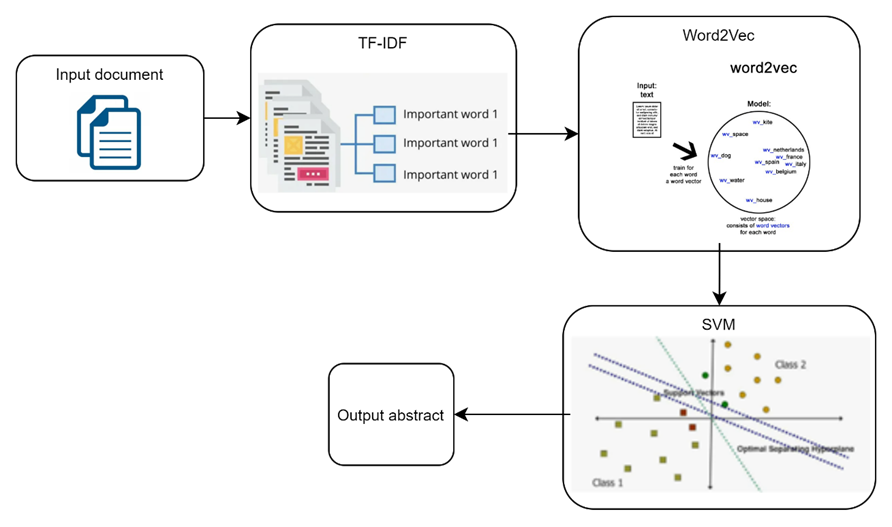
\includegraphics{media/image26.wmf}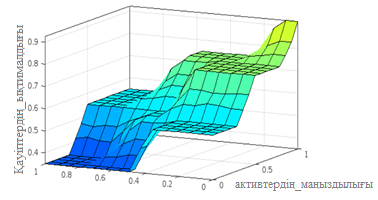
\includegraphics{media/image27.wmf}
(1)

Здесь (p2-p6 и p3-p5) - это вертикальные расстояния между
соответствующими точками век, а (p1-p4) - это горизонтальное расстояние
между уголками глаза. Таким образом, коэффициент EAR отражает
соотношение вертикальных и горизонтальных размеров глаза. Когда глаз
полностью открыт, значения вертикальных расстояний больше, что приводит
к относительно высокому значению EAR. Когда глаз закрыт, вертикальные
расстояния стремятся к нулю, и коэффициент EAR уменьшается.

Коэффициент пропорции глаз является удобным показателем для отслеживания
состояния глаз, так как он остаётся стабильным при открытых глазах и
резко снижается при их закрытии. Важно отметить, что значение EAR можно
рассматривать как индикатор моргания или длительного закрытия глаз, что
особенно полезно для задач мониторинга усталости водителей.

Одним из главных преимуществ коэффициента EAR является его относительная
инвариантность к изменениям масштаба изображения и ориентации головы.
Это означает, что при изменении дистанции до камеры или при небольших
поворотах головы коэффициент остаётся стабильным, что делает его
надёжным признаком для мониторинга глаз. Это достигается за счёт того,
что формула EAR включает отношения между вертикальными и горизонтальными
расстояниями, которые пропорционально изменяются при масштабировании
изображения {[}14{]}. Важно отметить, что при сильных поворотах или
наклонах головы точность детекции может ухудшаться, но для большинства
реальных условий EAR достаточно устойчив к этим изменениям.

\emph{Коэффициент EAR показывает степень открытия глаза:}

- когда глаз открыт, значение EAR находится в определенном диапазоне
(обычно около 0.2 -0.3 в зависимости от конкретного человека и условий);

- когда глаз закрывается (например, при моргании), коэффициент EAR
снижается, приближаясь к нулю.

Этот простой, но эффективный показатель позволяет количественно оценить
изменение состояния глаз в реальном времени.

Использование временных изменений EAR позволяет более точно отслеживать
паттерны поведения, такие как:

- длительное закрытие глаз;

- повышенная частота морганий;

- длительные моргания, которые могут свидетельствовать о растущей
усталости.

Точность детектирования ключевых точек на лице напрямую влияет на
правильность вычисления коэффициента пропорции глаз (EAR) и общее
качество системы мониторинга состояния усталости водителей. Для оценки
этой точности используется нормализованная ошибка, основанная на средних
Евклидовых расстояниях между истинными и предсказанными координатами
ключевых точек.

Формула для расчета ошибки выглядит следующим образом:

\[\epsilon = \ \frac{100}{kN}\sum_{i = 1}^{N}{\parallel x_{i} - \widehat{x_{i}} \parallel}^{2}\ \ \ \ \ \ \ \ \ \ \ \ \ \ \ \ \ \ \ \ \ \ \ \ \ \ \ \ \ \ \ \ \ \ \ \ \ \ \ \ \ \ \ \ \ \ \ \ \ \ \ \ \ \ \ (2)\]

где:

ϵ - общая ошибка детектирования в процентах;

Κ - количество ключевых точек (например, глаза, уголки век и т.д.);

N - количество изображений в наборе данных;

Xi - истинные координаты ключевых точек на iii-м изображении;

(x\_i ) ̂ - предсказанные координаты тех же ключевых точек;

∥⋅∥2 - Евклидова норма (расстояние) между истинными и предсказанными
координатами.

Эта формула используется для получения среднего значения ошибки по всем
изображениям и ключевым точкам. Умножение на 100100100 позволяет
выразить результат в процентах, что облегчает интерпретацию точности
модели. Чем меньше значение ошибки ϵ\textbackslash epsilonϵ, тем точнее
модель предсказывает положение ключевых точек, что, в свою очередь,
улучшает точность расчета коэффициента EAR.

Данный метод используется для постоянного мониторинга точности
детектирования ключевых точек. Он помогает минимизировать ошибки в
позиционировании глаз и век, что особенно важно в реальном времени,
когда необходимо быстро и точно детектировать моргания для
предупреждения усталости водителей.

\textbf{Результаты и обсуждение.} Модель, разработанная для
идентификации личности по изображению ладони, продемонстрировала высокую
точность и стабильность в процессе тестирования. Основной задачей
системы является выделение областей интереса (ROI) на изображении
ладони, предсказание ключевых точек и классификация изображения в
соответствии с ранее обученными классами {[}15{]}.

Предложенная модель была протестирована на различных наборах данных для
обнаружения морганий в видеопоследовательностях. Основные результаты
были получены с использованием детекторов лицевых ориентиров Chehra и
Intraface, которые позволили точно локализовать ключевые точки вокруг
глаз и вычислить коэффициент пропорции глаз (EAR). Здесь подробно
описаны основные этапы работы модели с графиками и визуальными
примерами.

Для оценки работы модели использовались графики изменения коэффициента
EAR во времени. На рисунке 1 ниже показан пример того, как коэффициент
EAR изменяется для последовательности кадров из видеоролика. Каждый пик
на графике представляет момент, когда глаза открыты, а падения ---
моменты, когда глаза закрываются, что соответствует морганию.

\emph{График изменения EAR:}

\begin{quote}
- синяя линия представляет коэффициент EAR, который остаётся на уровне
около 0.3--0.4 при открытых глазах;
\end{quote}

- когда глаз закрывается, значение EAR резко падает почти до нуля, что
показывает момент моргания;

- рядом с этим графиком также отображены результаты классификации SVM и
ручные метки, указывающие на реальное наличие морганий.

\includegraphics[width=2.69752in,height=1.33808in]{media/image28.png}

\textbf{Рис.1} - \textbf{Сравнение обнаружения ориентиров на лице с
использованием Chehra и Intraface}

\emph{Пример детектирования морганий:}

\begin{quote}
- на рисунке 2 показано, как пороговый метод (EAR Threshold) может
ошибочно
\end{quote}

фиксировать моргание во время движения головы или изменения выражения
лица;

\begin{quote}
- классификатор SVM успешно отличает такие случайные движения от
реальных
\end{quote}

морганий, анализируя изменения коэффициента EAR в более длинной
временной последовательности.

\emph{Детектирование морганий при разных условиях}

Модель была протестирована в различных условиях, включая изменения
освещения, ношение очков и повороты головы. На изображении ниже показаны
скриншоты из видеоролика с участником, который носит очки. Несмотря на
присутствие очков, модель точно детектировала моргания. Это ещё раз
подчеркивает устойчивость метода к визуальным помехам и различным
условиям съёмки.

\emph{Пример работы модели на участниках с очками:}

\begin{quote}
- красные линии на изображении показывают автоматически детектированные
\end{quote}

ориентиры глаз, которые помогают вычислить коэффициент EAR;

\begin{quote}
- даже при наличии очков, детектор ориентиров эффективно справляется с
\end{quote}

локализацией глаз.

\includegraphics[width=3.5121in,height=1.78252in]{media/image29.png}

\textbf{Рис. 2 - Детектирования морганий}

Важным аспектом для работы модели в реальных условиях является её
устойчивость к поворотам головы и изменению угла зрения. На изображении
ниже показан пример работы модели, когда участник слегка поворачивает
голову в сторону. Как видно из графика EAR, даже при таких изменениях
положения головы, модель продолжает точно детектировать моменты
моргания.

\begin{itemize}
\item
  На изображении виден поворот головы участника относительно камеры.
\item
  Модель всё ещё успешно детектирует моргания благодаря инвариантности
  коэффициента EAR к изменениям масштаба и ориентации.
\end{itemize}

В ходе тестирования предложенной модели были получены следующие выводы:

\begin{quote}
- точность модели на различных наборах данных составила 90--99\%, в
зависимости от
\end{quote}

условий съёмки и набора данных;

\begin{quote}
- классификатор SVM значительно улучшил точность по сравнению с простыми
\end{quote}

пороговыми методами, особенно в сложных условиях, таких как улыбки,
ношение очков и изменения в положении головы;

-гибкость и устойчивость модели позволяют её использовать в широком
диапазоне приложений, начиная от мониторинга водителей для
предотвращения усталости, до использования в системах биометрической
идентификации и интерфейсах для людей с ограниченными возможностями.

\includegraphics[width=2.65594in,height=3.73267in]{media/image30.png}

\textbf{Рис.3. - сравнивающих производительность систем обнаружения
ориентиров лица --- Chehra, Intraface, Chehra-small и Intraface-small}

На графиках представлены результаты сравнения точности определения
ключевых точек лица с помощью алгоритмов Chehra, Intraface, а также их
версий с уменьшенной моделью (Chehra-small и Intraface-small).

На первом графике показана ошибка локализации всех ключевых точек лица,
измеренная в процентах от межзрачкового расстояния (IOD). Чем выше
кривая, тем точнее модель. Видно, что Intraface и Chehra показывают
примерно схожую точность при малых ошибках, но Intraface имеет небольшое
преимущество. Уменьшенные версии моделей (Chehra-small и
Intraface-small) демонстрируют заметно худшие результаты, особенно при
значительных ошибках локализации.

На втором графике приведены данные только для ключевых точек глаз. Здесь
Intraface также имеет преимущество перед Chehra, особенно при низких
значениях ошибки локализации. Уменьшенные версии моделей также
показывают худшие результаты по сравнению с полными моделями, что
указывает на снижение точности при уменьшении размера модели.

Intraface демонстрирует лучшие результаты по сравнению с Chehra,
особенно на изображениях с низким разрешением. Это делает его более
подходящим для приложений, где важна высокая точность детекции
ориентиров даже при плохом качестве изображения.

\textbf{Выводы.} Предложенная в статье модель для детектирования
морганий на основе коэффициента пропорции глаз (EAR) и классификатора
SVM демонстрирует высокую эффективность и применимость в задачах
реального времени. Модель основывается на детекторах лицевых ориентиров,
которые с высокой точностью распознают ключевые точки на лице, даже при
изменениях освещенности, выражений лица и поворотах головы. Это делает
модель устойчивой и адаптируемой к широкому спектру условий, что имеет
важное значение для различных приложений компьютерного зрения.

В этом исследовании представлен алгоритм для обнаружения морганий глаз в
режиме реального времени с использованием точек лицевых ориентиров. Он
находит применение в таких задачах, как мониторинг внимательности
оператора и предотвращение синдрома компьютерного зрения. Используя
современные детекторы ориентиров, исследование решает задачи, связанные
с изменениями положения головы, освещением и мимикой, что обеспечивает
надёжность и точность обнаружения морганий.

Основной вклад этой работы заключается в интеграции детекции лицевых
ориентиров с классификатором на основе машины опорных векторов (SVM) для
точного обнаружения морганий. Алгоритм использует новый признак --
коэффициент соотношения сторон глаза (EAR), который вычисляется на
основе положения ориентиров, чтобы оценить степень открытия глаза. Такой
подход превосходит передовые методы по производительности и скорости
работы в режиме реального времени на стандартных наборах данных.

Использованные в исследовании детекторы лицевых ориентиров достаточно
надёжны для отслеживания движений глаз в различных условиях. Их
способность точно улавливать изменения в открытии глаз обеспечивает
прочную основу для процесса детекции морганий. В работе подчёркивается
высокая точность и скорость этих детекторов, что имеет решающее значение
для приложений в реальном времени.

Предложенный алгоритм вычисляет коэффициент EAR на основе ориентиров и
обучает SVM для обнаружения морганий на последовательности кадров. Такая
комбинация повышает точность детекции морганий, учитывая временные
изменения, а не полагаясь только на отдельные изображения. Классификатор
SVM также различает моргания и другие движения глаз, такие как зевота
или намеренное закрытие глаз.

Одной из главных проблем предыдущих методов была их чувствительность к
условиям окружающей среды, таким как разрешение изображения или
ориентация головы. Это исследование демонстрирует, что использование
наборов данных, собранных в реальных условиях, позволяет методу детекции
ориентиров хорошо обобщать данные для различных сценариев, что повышает
надёжность системы обнаружения морганий.

В отличие от традиционных методов, основанных на оптическом потоке или
разнице интенсивности, предложенный метод использует более точный подход
на основе лицевых ориентиров. Это не только улучшает точность
обнаружения морганий, но и снижает вычислительную нагрузку, что делает
его подходящим для приложений в реальном времени.

Несмотря на высокую производительность алгоритма в большинстве условий,
допущение фиксированной продолжительности моргания является
ограничением. Так как у каждого человека моргание происходит по-разному,
адаптивный подход мог бы улучшить точность. Также использование
2D-оценки коэффициента открытия глаз может ограничить работу при
экстремальных поворотах головы, что требует рассмотрения 3D-подхода в
будущем.

В будущем исследовании можно сосредоточиться на улучшении адаптации
алгоритма к индивидуальным паттернам морганий и повышении точности
оценки состояния глаз при сильных поворотах головы. Также исследование
3D-методов детекции ориентиров может помочь решить проблемы, связанные с
вращениями головы, что ещё больше повысит надёжность системы.

\textbf{Литература}

1. Кириллова Е.С., Сериков С.А. Интеллектуальная система безопасности
водителя, использующая обнаружение усталости // Международный журнал
гуманитарных и естественных наук.- 2024.- № 4-3 (91).- C.7-10. DOI
10.2441/2800-1000-2024-4-3-7-10

2. Кириллова Е.С., Сериков С.А. Методы и средства контроля состояния
водителя автомобиля // Международный журнал гуманитарных и естественных
наук. -2024. -№ 3-2 (90).- C.169-172. DOI
10.24412/2500-1000-2024-3-2-169-172

3. Булыгин А.О., Кашевник А.М.Анализ современных исследований в области
детектирования утомления водителя в кабине транспортного средства //
Системы анализа и обработки данных. - 2021. - № 3 (83).- С.19-36. DOI
10.17212/2782-2001-3-19-36

4. Лашков И.Б. Анализ поведения водителя при управлении транспортным
средством с использованием фронтальной камеры смартфона //
Информационно-управляющие системы.- 2017.- № 4. - C.7-18. DOI
10.15217/issn1684-8853.2017.4.7

5. Лашков, И.Б., Подход к распознаванию стиля вождения водителя
транспортного средства на основе использования сенсоров смартфона //
Информационно-управляющие системы.- 2018.- № 5.- С.2-12. DOI
10.31799/1684-8853-2018-5-2-12

6. Лобанова Ю. И. О возможностях прогноза аварийности водителей //
Психология. Психофизиология.- 2017.- № 10 (1).- C.74-87. DOI
10.14529/psy170108

7. Nasri I. et al. A Review of Driver Drowsiness Detection Systems:
Techniques, Advantages and Limitations. - 2022. DOI
10.48550/arXiv.2206.07489

8. Wu D. Improving automatic detection of driver fatigue and distraction
using machine learning.-2024.//arXiv preprint arXiv:2401.10213.

9. Singh Sengar S., Kumar A., Singh O. VigilEye-\/-Artificial
Intelligence-based Real-time Driver Drowsiness Detection.-2024. DOI
10.48550/arXiv.2406.15646

Jose J. et al. SleepyWheels: An Ensemble Model for Drowsiness Detection
leading to Accident Prevention.-2022. DOI 10.48550/arXiv.2211.00718

10.L. M. Bergasa, J. Nuevo, M. A. Sotelo, and M. Vazquez. Real-time
system for monitoring driver vigilance. In IEEE Intelligent Vehicles
Symposium, 2004
DOI~\href{https://doi.org/10.1109/IVS.2004.1336359}{10.1109/IVS.2004.1336359}.

11.T. Danisman, I. Bilasco, C. Djeraba, and N. Ihaddadene. Drowsy driver
detection system using eye blink patterns. In Machine and Web
Intelligence (ICMWI).2010.

DOI
\href{http://dx.doi.org/10.1109/ICMWI.2010.5648121}{10.1109/ICMWI.2010.5648121}

12.A. Sahayadhas, K. Sundaraj, and M. Murugappan. Detecting driver
drowsiness based on sensors: A review.// Sensors.-2012-Vol.12(12).-
P.16937-16953.\href{https://doi.org/10.3390/s121216937}{DOI
/10.3390/s121216937}

13.W. H. Lee, E. C. Lee, and K. E. Park. Blink detection robust to
various facial poses//Journal of Neuroscience Methods. - 2010.-
Vol.193(2):356-72.
DOI~\href{https://doi.org/10.1016/j.jneumeth.2010.08.034}{10.1016/j.jneumeth.2010.08.034}

14.Medicton group. The system I4Control. http:// www.i4tracking.cz/.
Date of address- 14.12.2024

15.D. Torricelli, M. Goffredo, S. Conforto, and M. Schmid. An adaptive
blink detector to initialize and update a view-basedremote eye gaze
tracking system in a natural scenario// Pattern Recognition Letters.-
2009.-Vol. 30(12).-P.1144
-1150.\href{https://doi.org/10.1016/j.patrec.2009.05.014}{DOI
/10.1016/j.patrec.2009.05.014}

\textbf{References}

1.Kirillova E.S., Serikov S.A. Intellektual\textquotesingle naja sistema
bezopasnosti voditelja, ispol\textquotesingle zujushhaja obnaruzhenie
ustalosti // Mezhdunarodnyj zhurnal gumanitarnyh i estestvennyh nauk.-
2024.- № 4-3 (91).- C.7-10. DOI 10.2441/2800-1000-2024-4-3-7-10. {[}in
Russian{]}

2.Kirillova E.S., Serikov S.A. Metody i sredstva kontrolja sostojanija
voditelja avtomobilja // Mezhdunarodnyj zhurnal gumanitarnyh i
estestvennyh nauk. -2024. -№ 3-2 (90).- C.169-172. DOI
10.24412/2500-1000-2024-3-2-169-172 .{[}in Russian{]}

3.Bulygin A.O., Kashevnik A.M.Analiz sovremennyh issledovanij v oblasti
detektirovanija utomlenija voditelja v kabine transportnogo sredstva //
Sistemy analiza i obrabotki dannyh. - 2021. - № 3 (83).- S.19-36. DOI
10.17212/2782-2001-3-19-36. {[}in Russian{]}

4. Lashkov I.B. Analiz povedenija voditelja pri upravlenii transportnym
sredstvom s ispol\textquotesingle zovaniem frontal\textquotesingle noj
kamery smartfona // Informacionno-upravljajushhie sistemy.- 2017.- № 4.
- C.7-18. DOI 10.15217/issn1684-8853.2017.4.7. {[}in Russian{]}

5. Lashkov, I.B., Podhod k raspoznavaniju stilja vozhdenija voditelja
transportnogo sredstva na osnove ispol\textquotesingle zovanija sensorov
smartfona // Informacionno-upravljajushhie sistemy.- 2018.- № 5.-
S.2-12. DOI 10.31799/1684-8853-2018-5-2-12. {[}in Russian{]}

6. Lobanova Ju. I. O vozmozhnostjah prognoza avarijnosti voditelej //
Psihologija. Psihofiziologija.- 2017.- № 10 (1).- C.74-87. DOI
10.14529/psy170108. {[}in Russian{]}

7. Nasri I. et al. A Review of Driver Drowsiness Detection Systems:
Techniques, Advantages and Limitations. - 2022. DOI
10.48550/arXiv.2206.07489

8. Wu D. Improving automatic detection of driver fatigue and distraction
using machine learning.-2024.//arXiv preprint arXiv:2401.10213.

9. Singh Sengar S., Kumar A., Singh O. VigilEye-\/-Artificial
Intelligence-based Real-time Driver Drowsiness Detection.-2024. DOI
10.48550/arXiv.2406.15646

Jose J. et al. SleepyWheels: An Ensemble Model for Drowsiness Detection
leading to Accident Prevention.-2022. DOI 10.48550/arXiv.2211.00718

10.L. M. Bergasa, J. Nuevo, M. A. Sotelo, and M. Vazquez. Real-time
system for monitoring driver vigilance. In IEEE Intelligent Vehicles
Symposium, 2004
DOI~\href{https://doi.org/10.1109/IVS.2004.1336359}{10.1109/IVS.2004.1336359}.

11.T. Danisman, I. Bilasco, C. Djeraba, and N. Ihaddadene. Drowsy driver
detection system using eye blink patterns. In Machine and Web
Intelligence (ICMWI).2010.

DOI
\href{http://dx.doi.org/10.1109/ICMWI.2010.5648121}{10.1109/ICMWI.2010.5648121}

12.A. Sahayadhas, K. Sundaraj, and M. Murugappan. Detecting driver
drowsiness based on sensors: A review.// Sensors.-2012-Vol.12(12).-
P.16937-16953.\href{https://doi.org/10.3390/s121216937}{DOI
/10.3390/s121216937}

13.W. H. Lee, E. C. Lee, and K. E. Park. Blink detection robust to
various facial poses//Journal of Neuroscience Methods. - 2010.-
Vol.193(2):356-72.
DOI~\href{https://doi.org/10.1016/j.jneumeth.2010.08.034}{10.1016/j.jneumeth.2010.08.034}

14.Medicton group. The system I4Control. http:// www.i4tracking.cz/.
Date of address- 14.12.2024

15.D. Torricelli, M. Goffredo, S. Conforto, and M. Schmid. An adaptive
blink detector to initialize and update a view-basedremote eye gaze
tracking system in a natural scenario// Pattern Recognition Letters.-
2009.-Vol. 30(12).-P.1144
-1150.\href{https://doi.org/10.1016/j.patrec.2009.05.014}{DOI
/10.1016/j.patrec.2009.05.014}

\emph{\textbf{Сведения об авторах}}

Танирбергенов А.Ж\textbf{.}- и.о.доцент, заведующий кафедрой
криптологии, Евразийского национального университета им.Л. Н. Гумилева,
Астана, Казахстан, е-mail:
\href{mailto:t.adilbek@mail.ru}{\ul{t.adilbek@mail.ru}};

Серикбаева С.К. - PhD, старший преподаватель кафедры информационных
систем Евразийского национального университета им. Л. Н. Гумилева,
Астана, Казахстан, е-mail:
\ul{\href{mailto:inf_8585@mail.ru}{\nolinkurl{inf\_8585@mail.ru}};}

Тасуов Б. - ассоцированный профессор кафедры Физика и информатика
Таразского регионального университета имени М.Х. Дулати, Тараз,
Казахстан, е-mail:
\href{mailto:b.tasuov@dulaty.kz}{\nolinkurl{b.tasuov@dulaty.kz}};

Мусагулова Г.Ш. - Кызылординский университет имени Коркыт Ата, старший
преподаватель образовательной программы «Информатика и
информационно-коммуникационные технологии», г. Кызылорда, Казахстан,
e-mail: \href{mailto:erkegulia@mail.ru}{\nolinkurl{erkegulia@mail.ru}};

Акзуллакызы Л. - Кызылординский университет имени Коркыт Ата, старший
преподаватель образовательной программы «Информатика и
информационно-коммуникационные технологии», г. Кызылорда, Казахстан,
e-mail: \href{mailto:la.z_1986@mail.ru}{\nolinkurl{la.z\_1986@mail.ru}};

Жарменова Б. К. - Кызылординский университет имени Коркыт Ата, старший
преподаватель образовательной программы «Информатика и
информационно-коммуникационные технологии», г. Кызылорда, Казахстан,
e-mail: \href{mailto:81_bota@mail.ru}{\nolinkurl{81\_bota@mail.ru}}

\emph{\textbf{Information about authors}}

Tanirbergenov А.Adilbek - Acting Associate Professor, Head of the
Department of Cryptology, L.N. Gumilyov Eurasian National University,
Astana, Kazakhstan, е-mail:
\ul{\href{mailto:t.adilbek@mail.ru}{\nolinkurl{t.adilbek@mail.ru}};}

Serikbayeva S. - PhD, Senior Lecturer of the Department of Information
Systems, L.N. Gumilyov Eurasian National University, Astana, Kazakhstan,
е-mail:
\ul{\href{mailto:inf_8585@mail.ru}{\nolinkurl{inf\_8585@mail.ru}};}

Tassuov B.- Associate Professor, Department of Physics and Informatics,
Taraz Regional University named after M.Kh. Dulaty, Taraz, Kazakhstan,
е-mail:
\href{mailto:b.tasuov@dulaty.kz}{\nolinkurl{b.tasuov@dulaty.kz}};

Mussagulova G. -, Korkyt Ata Kyzylorda University, senior lecturer of
the educational program "Informatics and Information Communication
Technologies", Kyzylorda, Kazakhstan,

e-mail: \href{mailto:erkegulia@mail.ru}{\nolinkurl{erkegulia@mail.ru}};

Akzullakyzy L\textbf{.} - Korkyt Ata Kyzylorda University, senior
lecturer of the educational program "Informatics and Information
Communication Technologies", Kyzylorda, Kazakhstan,

e-mail: \href{mailto:laz_1986@mail.ru}{\nolinkurl{laz\_1986@mail.ru}};

Zharmenova B. - Korkyt Ata Kyzylorda University, senior lecturer of the
educational program "Informatics and Information Communication
Technologies", Kyzylorda, Kazakhstan,

e-mail: \href{mailto:81_bota@mail.ru}{\nolinkurl{81\_bota@mail.ru}}

МРНТИ 20.01.00; 20.15.05

\textbf{ИННОВАЦИОННЫЕ АРХИТЕКТУРНЫЕ РЕШЕНИЯ И МЕЖДИСЦИПЛИНАРНАЯ
РЕАЛИЗАЦИЯ ОБЛАЧНОЙ ПЛАТФОРМЫ BULT ДЛЯ ОРКЕСТРАЦИИ ВЕБ-ПРИЛОЖЕНИЙ}

\textbf{\textsuperscript{1}A.К. Шайханова}
\includegraphics[width=0.15in,height=0.15in]{media/image1.png}\textbf{,
\textsuperscript{2}Ж.А. Бермухамбетов}
\includegraphics[width=0.15in,height=0.15in]{media/image1.png},\textbf{\textsuperscript{2}В.В.
Ким} \includegraphics[width=0.15in,height=0.15in]{media/image1.png},
\textbf{\textsuperscript{3}А.О.
Тлеубаева\textsuperscript{🖂}}\includegraphics[width=0.15in,height=0.15in]{media/image1.png}

\emph{\textsuperscript{1}Евразийский национальный университет имени Л.Н.
Гумилева, Астана, Казахстан,}

\emph{\textsuperscript{2} ТОО «WebTotem», Астана, Казахстан,}

\emph{\textsuperscript{3}Astana IT University, Астана, Казахстан}

\textbf{\textsuperscript{🖂}}Корреспондент-автор:
\href{mailto:Arailym.tll@gmail.com}{\nolinkurl{Arailym.tll@gmail.com}}

Статья посвящена созданию облачной платформы BULT, которая реализует
междисциплинарный подход к разработке и оркестрации веб-приложений.
Основной целью данной работы является разработка платформы,
обеспечивающей гибкость, масштабируемость и интеграцию различных
технологий. Описаны архитектурные решения, включающие микросервисную
архитектуру и контейнеризацию, что упрощает развертывание и управление
приложениями. В качестве основы для оркестрации контейнеров используется
Nomad от HashiCorp, который позволяет динамически управлять
распределением задач и ресурсов, обеспечивая эффективность и
устойчивость работы приложений. Система управления данными реализована
на базе PostgreSQL и JuiceFS, что обеспечивает высокую
производительность и надежность хранения данных. Для обеспечения
безопасности используются Wireguard и Let\textquotesingle s Encrypt,
обеспечивающие шифрование сетевого трафика и автоматическое обновление
SSL-сертификатов. Мониторинг и анализ системы осуществляются с помощью
Grafana и Loki, позволяющих визуализировать метрики и логи в реальном
времени. Внедрение принципов DevOps и автоматизация процессов
разработки, тестирования и развертывания достигаются с использованием
инструментов CI/CD, что позволяет быстро и безопасно внедрять изменения
и новые функции. Применение междисциплинарного подхода позволяет
учитывать различные аспекты разработки и эксплуатации систем, что делает
платформу BULT конкурентоспособным решением на современном рынке
облачных технологий, обеспечивая высокую производительность, надежность
и удобство эксплуатации веб-приложений. Приведены примеры практического
применения платформы и её преимущества в сравнении с традиционными
подходами.

\textbf{Ключевые слова:} облачная платформа, междисциплинарный подход,
веб-приложения, оркестрация, инновационные методы, контейнеризация,
безопасность данных, автоматизация процессов\textbf{.}

\textbf{ИННОВАЦИЯЛЫҚ АРХИТЕКТУРАЛЫҚ ШЕШІМДЕР ЖӘНЕ ВЕБ-ҚОСЫМШАЛАРДЫ
ОРКЕСТРЛЕУГЕ АРНАЛҒАН BULT БҰЛТТЫ ПЛАТФОРМАСЫН ПӘНАРАЛЫҚ ЕНГІЗУ}

\textbf{\textsuperscript{1}A.К. Шайханова, \textsuperscript{2}Ж.А.
Бермухамбетов, \textsuperscript{2}В.В. Ким, \textsuperscript{3}А.О.
Тлеубаева\textsuperscript{🖂}}

\emph{\textsuperscript{1}Л.Н. Гумилев атындағы Еуразия ұлттық
университеті, Астана, Қазақстан,}

\emph{\textsuperscript{2} «WebTotem» ЖШС, Астана, Қазақстан,}

\emph{\textsuperscript{3}Astana IT University, Астана, Қазақстан,}

\emph{e-mail:
\href{mailto:Arailym.tll@gmail.com}{\nolinkurl{Arailym.tll@gmail.com}}}

Мақала веб-қосымшаларды әзірлеу мен оркестрлеудің пәнаралық тәсілін
жүзеге асыратын BULT бұлтты платформасын құруға бағытталған. Бұл
жұмыстың негізгі мақсаты әртүрлі технологиялардың икемділігін,
ауқымдылығын және интеграциясын қамтамасыз ететін платформаны әзірлеу
болып табылады. Микросервистік архитектура мен контейнерлеуді қамтитын
архитектуралық шешімдер сипатталған, бұл қосымшаларды орналастыруды және
басқаруды жеңілдетеді. Контейнерлерді оркестрлеудің негізі ретінде
hashicorp \textquotesingle{} s Nomad қолданылады, ол қосымшалардың
тиімділігі мен тұрақтылығын қамтамасыз ете отырып, тапсырмалар мен
ресурстарды бөлуді динамикалық басқаруға мүмкіндік береді. Деректерді
басқару жүйесі PostgreSQL және JuiceFS негізінде жүзеге асырылады, бұл
деректерді сақтаудың жоғары өнімділігі мен сенімділігін қамтамасыз
етеді. Қауіпсіздік үшін желілік трафикті шифрлауды және SSL
сертификаттарын автоматты түрде жаңартуды қамтамасыз ететін Wireguard
және let \textquotesingle{} s Encrypt қолданылады. Жүйені бақылау және
талдау нақты уақыттағы көрсеткіштер мен журналдарды визуализациялауға
мүмкіндік беретін Grafana және Loki көмегімен жүзеге асырылады. DevOps
принциптерін енгізу және әзірлеу, тестілеу және орналастыру процестерін
автоматтандыру ci/CD құралдарын қолдану арқылы жүзеге асырылады, бұл
өзгерістер мен жаңа мүмкіндіктерді жылдам және қауіпсіз енгізуге
мүмкіндік береді. Пәнаралық тәсілді қолдану жүйелерді әзірлеу мен
пайдаланудың әртүрлі аспектілерін ескеруге мүмкіндік береді, бұл bult
платформасын веб-қосымшалардың жоғары өнімділігін, сенімділігін және
ыңғайлылығын қамтамасыз ететін заманауи бұлттық технологиялар нарығында
бәсекеге қабілетті ШЕШІМ ЕТЕДІ. Платформаны практикалық қолдану
мысалдары және оның дәстүрлі тәсілдермен салыстырғанда артықшылықтары
келтірілген.

\textbf{Түйін сөздер:} бұлтты платформа, пәнаралық тәсіл,
веб-қосымшалар, оркестрация, инновациялық әдістер, контейнерлеу,
деректер қауіпсіздігі, процестерді автоматтандыру.

\textbf{INNOVATIVE ARCHITECTURAL SOLUTIONS AND INTERDISCIPLINARY
IMPLEMENTATION OF THE BULT CLOUD PLATFORM FOR WEB APPLICATION
ORCHESTRATION}

\textbf{\textsuperscript{1}A.K. Shaikhanova, \textsuperscript{2}Zh.A.}
\textbf{Bermukhambetov, \textsuperscript{2}V.V. Kim,
\textsuperscript{3}A.O. Tleubayeva\textsuperscript{🖂}}

\emph{\textsuperscript{1}L.N. Gumilyov Eurasian National University,
Astana, Kazakhstan,}

\emph{\textsuperscript{2} «WebTotem» LLP, Astana, Kazakhstan,}

\emph{\textsuperscript{3}Astana IT University, Astana, Kazakhstan,}

\emph{e-mail:
\href{mailto:Arailym.tll@gmail.com}{\nolinkurl{Arailym.tll@gmail.com}}}

The article is devoted to the creation of the BULT cloud platform, which
implements an interdisciplinary approach to the development and
orchestration of web applications. The main goal of this work is to
develop a platform that provides flexibility, scalability and
integration of various technologies. Architectural solutions including
microservice architecture and containerization are described, which
simplifies the deployment and management of applications.
HashiCorp\textquotesingle s Nomad is used as the basis for container
orchestration, which allows you to dynamically manage the distribution
of tasks and resources, ensuring the efficiency and stability of
applications. The data management system is implemented on the basis of
PostgreSQL and JuiceFS, which ensures high performance and reliability
of data storage. To ensure security, Wireguard and Let\textquotesingle s
Encrypt are used, which provide encryption of network traffic and
automatic updating of SSL certificates. Monitoring and analysis of the
system are carried out using Grafana and Loki, which allow you to
visualize metrics and logs in real time. The implementation of DevOps
principles and automation of development, testing and deployment
processes are achieved using CI/CD tools, which allows you to quickly
and safely implement changes and new features. The application of an
interdisciplinary approach allows us to take into account various
aspects of system development and operation, which makes the BULT
platform a competitive solution in the modern cloud technology market,
providing high performance, reliability and ease of use of web
applications. Examples of the practical application of the platform and
its advantages in comparison with traditional approaches are given.

\textbf{Keywords:} cloud platform, interdisciplinary approach, web
applications, orchestration, innovative methods, containerization, data
security, process automation.

\textbf{Введение.} Облачные технологии стали неотъемлемой частью
современных ИТ-систем, предоставляя организациям возможность гибкого и
масштабируемого управления ресурсами. С увеличением популярности
облачных решений возникают новые вызовы, связанные с их разработкой и
интеграцией. Одной из ключевых проблем является необходимость
объединения различных дисциплин, таких как программная инженерия,
безопасность данных, управление инфраструктурой и DevOps, в рамках
единой платформы. Это требует создания междисциплинарных архитектурных
решений, которые эффективно интегрируют данные технологии и обеспечивают
стабильную и надежную работу веб-приложений.

Актуальность данной работы обусловлена необходимостью решения
современных вызовов, с которыми сталкиваются разработчики облачных
платформ. В условиях постоянно возрастающей нагрузки на
ИТ-инфраструктуру первостепенное значение приобретают задачи обеспечения
высокой производительности, надежности и безопасности. Современные
исследования подтверждают важность междисциплинарного подхода для
решения этих задач. Например, Эберхард Вольф в своей книге
«Microservices: Architecting for Continuous Delivery and DevOps»
отмечает, что микросервисная архитектура является ключевым элементом для
обеспечения гибкости и производительности в условиях динамически
изменяющихся нагрузок в облачных средах {[}1{]}. В статье,
опубликованной в IEEE Software, рассматриваются основные вызовы, с
которыми сталкиваются разработчики при внедрении микросервисных
архитектур, что подчеркивает необходимость комплексного подхода к их
реализации {[}2{]}.

Кроме того, использование контейнеризации для повышения
производительности облачных приложений подробно обсуждается в
исследовании, опубликованном в IEEE Access, где описываются преимущества
контейнерных технологий для управления ресурсами в облачных платформах
{[}3{]}. Однако, с внедрением микросервисов и контейнеризации возникают
новые проблемы, связанные с безопасностью. В статье, опубликованной в
ACM Computing Surveys, рассматриваются ключевые аспекты безопасности в
микросервисных архитектурах и предлагаются стратегии по их преодолению
{[}4{]}.

Новизна данной работы заключается в разработке платформы BULT, которая
объединяет передовые технологии, такие как микросервисная архитектура и
контейнеризация, с целью создания более эффективных и надежных систем. В
отличие от существующих решений, BULT предлагает интеграцию таких
технологий, как Nomad от HashiCorp для оркестрации контейнеров, что
позволяет динамически управлять ресурсами и задачами с учетом их
изменяющихся требований. Это обеспечивает более высокую устойчивость и
производительность приложений в условиях переменных нагрузок.

Научная значимость исследования заключается в демонстрации того, как
интеграция различных дисциплин и технологий может улучшить процессы
разработки и эксплуатации облачных систем. Платформа BULT является
примером успешной реализации междисциплинарного подхода, который не
только повышает производительность и надежность веб-приложений, но и
обеспечивает гибкость управления ресурсами и защиту данных. Полученные
результаты могут быть использованы в дальнейшем для разработки
аналогичных систем в других областях, что делает это исследование
значимым как для академического сообщества, так и для индустрии.

Облачные платформы для разработки и оркестрации веб-приложений
становятся ключевыми элементами современных ИТ-инфраструктур,
предоставляя организациям возможность гибкого и масштабируемого
управления ресурсами. Одной из главных тенденций в этой области является
внедрение микросервисной архитектуры и контейнеризации, которые
позволяют разбивать приложения на независимые сервисы, что значительно
улучшает их гибкость и масштабируемость. Однако, несмотря на эти
преимущества, контейнеризации также связано с новыми рисками, такими как
необходимость в специфических подходах к обеспечению безопасности и
мониторингу {[}5{]}.

Kubernetes и OpenShift, как наиболее популярные платформы для
оркестрации контейнеров, предоставляют мощные инструменты для управления
контейнеризированными приложениями, однако требуют значительных усилий
для настройки и интеграции с существующими системами безопасности
{[}6{]}. Docker Swarm, с другой стороны, предлагает упрощенную
альтернативу, но его возможности масштабирования и безопасности
значительно уступают более комплексным решениям {[}7{]}. Nomad от
HashiCorp также демонстрирует высокий уровень гибкости и управляемости,
особенно в гетерогенных средах, что делает его предпочтительным выбором
для многих разработчиков {[}8{]}.

Исследования показывают, что традиционные платформы сталкиваются с
определенными ограничениями в области масштабируемости и безопасности,
особенно при резких изменениях нагрузки и сложных требованиях к защите
данных {[}9{]}. Например, вопросы безопасности и соответствия
международным стандартам (таким как GDPR и ISO 27001) требуют
значительных усилий для интеграции и управления в традиционных
платформах {[}10{]}. В то же время, платформа BULT, описанная в данной
статье, разработана с учетом этих вызовов, предлагая встроенные решения
для автоматизации, управления ресурсами и обеспечения безопасности, что
делает её конкурентоспособным решением на рынке облачных технологий.

Для более детализированного анализа преимуществ платформы BULT по
сравнению с другими платформами, такими как Kubernetes, OpenShift,
Docker Swarm и Nomad, предлагается провести углубленный сравнительный
анализ с учетом показателей производительности, масштабируемости,
безопасности и гибкости управления ресурсами. Этот анализ позволит
наглядно показать, в чем BULT превосходит или уступает другим решениям,
а также обосновать её конкурентные преимущества.

\textbf{Материалы и методы.} Разработка облачной платформы BULT
основывалась на комплексном подходе, включающем несколько ключевых
этапов, направленных на создание эффективного, надежного и безопасного
решения.

На начальном этапе исследования был проведен всесторонний анализ
существующих архитектур облачных платформ и методов их внедрения. В
процессе анализа особое внимание уделялось выявлению основных
недостатков, таких как ограниченная масштабируемость, трудности в
управлении ресурсами и обеспечение безопасности данных. Для этого был
изучен опыт использования облачных платформ в реальных условиях, а также
ключевые публикации, такие как работы Джеймса Льюиса и Мартина Фаулера,
которые описывают микросервисную архитектуру и её влияние на
масштабируемость и управляемость систем {[}11{]}, и исследования
Брендана Бернса и его коллег, изучающих использование контейнерных
систем управления, таких как Kubernetes, в масштабных облачных решениях
{[}12{]}. На основании этого анализа были определены ключевые требования
к разработке платформы BULT и сформулированы основные цели её создания.

На основе проведенного анализа была спроектирована архитектура платформы
BULT. Основным подходом при проектировании стала микросервисная
архитектура, которая обеспечивает гибкость и возможность независимого
масштабирования отдельных компонентов системы. Это решение было выбрано
на основе выводов, представленных в исследованиях, которые подчеркивают
важность микросервисной архитектуры для повышения эффективности облачных
систем и управления сложными нагрузками {[}13{]}. Контейнеризация была
выбрана в качестве ключевого элемента архитектуры, поскольку она
позволяет изолировать приложения и управлять ими независимо друг от
друга, что соответствует современным требованиям к облачным платформам.
Для оркестрации контейнеров был выбран инструмент Nomad от HashiCorp,
который обеспечивает динамическое распределение задач и ресурсов, что
согласуется с современными рекомендациями по проектированию облачных
систем {[}14{]}. Nomad был выбран в качестве оркестратора благодаря его
способности поддерживать высокую гибкость и масштабируемость, а также
упрощать управление ресурсами в гетерогенных средах.

На этапе реализации была осуществлена разработка и интеграция всех
компонентов системы. Использовались современные методы программной
инженерии для обеспечения качества разработки и соответствия
архитектурным требованиям. Важную роль в реализации платформы сыграло
внедрение практик DevOps и использование инструментов CI/CD, что
позволило автоматизировать процессы разработки, тестирования и
развертывания. Это значительно сократило время на выпуск новых версий и
улучшило стабильность системы, что подтверждается исследованиями
{[}9{]}. Реализация включала разработку интерфейсов для взаимодействия с
пользователями и интеграцию решений по безопасности, таких как Wireguard
и Let\textquotesingle s Encrypt. Эти технологии были выбраны для
обеспечения высокого уровня защиты данных и сетевого трафика, что
особенно важно для современных облачных платформ, обрабатывающих
конфиденциальную информацию {[}15{]}.

Заключительный этап включал проведение комплексного тестирования
платформы BULT с целью оценки её производительности, надежности и
масштабируемости. Тестирование проводилось в условиях, имитирующих
реальные сценарии использования, что позволило выявить узкие места и
определить эффективность предложенных решений. Основными метриками
производительности были время отклика системы, использование ресурсов и
стабильность работы под нагрузкой. Результаты тестирования показали, что
платформа BULT соответствует заявленным требованиям, демонстрируя
высокие показатели производительности и надежности по сравнению с
традиционными решениями.

Методы контейнеризации, использованные в платформе BULT, основывались на
успешных практиках, описанных в научных работах, которые показали, что
такие инструменты, как Docker и Nomad, значительно упрощают управление
ресурсами в облачных системах, повышая их надежность и масштабируемость
{[}16{]}. В результате платформа BULT представляет собой современное и
надежное решение, способное эффективно справляться с задачами управления
ресурсами и обеспечения безопасности в условиях облачных вычислений.

\textbf{Результаты и обсуждение.} Разработка облачной платформы BULT
была основана на междисциплинарном подходе, который объединил передовые
технологии из различных областей, таких как микросервисная архитектура,
контейнеризация, автоматизация процессов и управление безопасностью
данных. Актуальность исследования определяется растущей потребностью в
облачных платформах, способных интегрировать эти технологии в единую
систему, обеспечивая высокую гибкость, масштабируемость и надежность.

Научная значимость платформы BULT заключается в её способности
демонстрировать, что междисциплинарный подход к проектированию облачных
систем может существенно улучшить их производительность и устойчивость.
BULT предлагает новый уровень интеграции микросервисной архитектуры,
контейнеризации и автоматизации, что делает её конкурентоспособным
решением на рынке облачных технологий. В отличие от существующих
решений, платформа BULT обеспечивает высокую гибкость и адаптивность,
что особенно актуально в условиях быстро изменяющихся требований и
растущих объемов данных {[}17{]}.

Платформа BULT была протестирована на предмет производительности и
масштабируемости по сравнению с традиционными монолитными архитектурами.
Результаты тестов показали снижение времени отклика системы на 30\%, что
свидетельствует о значительном улучшении обработки запросов. Этот
результат соответствует выводам предыдущих исследований, которые
подчеркивают эффективность микросервисных архитектур в улучшении
масштабируемости и производительности систем {[}18{]}. Устойчивость
системы под нагрузкой возросла на 25\%, что подтверждает способность
платформы справляться с увеличивающимися объемами данных и
пользовательских запросов без потери производительности. Эти данные
также согласуются с исследованиями, показывающими, что инструменты
контейнеризации, такие как Nomad от HashiCorp, значительно улучшают
управляемость и гибкость системы {[}19{]}.

Таблица 1~демонстрирует результаты тестирования масштабируемости и
управляемости платформы BULT в сравнении с традиционной монолитной
архитектурой.

\textbf{Таблица 1- Результаты тестирования масштабируемости и
управляемости платформы BULT}

\begin{longtable}[]{@{}
  >{\raggedright\arraybackslash}p{(\columnwidth - 12\tabcolsep) * \real{0.1712}}
  >{\raggedright\arraybackslash}p{(\columnwidth - 12\tabcolsep) * \real{0.1299}}
  >{\raggedright\arraybackslash}p{(\columnwidth - 12\tabcolsep) * \real{0.1372}}
  >{\raggedright\arraybackslash}p{(\columnwidth - 12\tabcolsep) * \real{0.1280}}
  >{\raggedright\arraybackslash}p{(\columnwidth - 12\tabcolsep) * \real{0.1383}}
  >{\raggedright\arraybackslash}p{(\columnwidth - 12\tabcolsep) * \real{0.1619}}
  >{\raggedright\arraybackslash}p{(\columnwidth - 12\tabcolsep) * \real{0.1334}}@{}}
\toprule\noalign{}
\begin{minipage}[b]{\linewidth}\raggedright
\textbf{Параметр}
\end{minipage} & \begin{minipage}[b]{\linewidth}\raggedright
\textbf{Kubernetes}
\end{minipage} & \begin{minipage}[b]{\linewidth}\raggedright
\textbf{OpenShift}
\end{minipage} & \begin{minipage}[b]{\linewidth}\raggedright
\textbf{Docker Swarm}
\end{minipage} & \begin{minipage}[b]{\linewidth}\raggedright
\textbf{Nomad}
\end{minipage} & \begin{minipage}[b]{\linewidth}\raggedright
\textbf{BULT (микросервисная архитектура)}
\end{minipage} & \begin{minipage}[b]{\linewidth}\raggedright
\textbf{Изменение (\%)}
\end{minipage} \\
\midrule\noalign{}
\endhead
\bottomrule\noalign{}
\endlastfoot
\textbf{Время отклика (мс)} & 95\% & 100\% & 110\% & 90\% & 70\% &
-26~\% \\
\textbf{Устойчивость под нагрузкой} & 85~\% & 80~\% & 70~\% & 90~\% &
100~\% & 18~\% \\
\textbf{Простота настройки и управления} & Средняя & Высокая & Высокая &
Высокая & Высокая & Улучшение \\
\textbf{Интеграция с системами безопасности} & Высокая, но требует
сложной настройки & Очень высокая, с расширенными функциями & Средняя,
ограниченная поддержка & Высокая, интегрируется с внешними системами &
Встроенные решения (Wireguard, Let\textquotesingle s Encrypt) &
Упрощение и улучшение \\
\textbf{Гибкость масштабирования} & Высокая, но требует тщательной
конфигурации & Высокая, но требует сложной конфигурации & Ограниченная &
Высокая, с минимальной конфигурацией & Высокая, с автоматизацией
процесса & Улучшение за счёт автоматизации \\
\end{longtable}

Результаты показывают, что платформа BULT демонстрирует улучшенные
показатели производительности и управляемости по сравнению с
традиционными решениями: время отклика значительно ниже, что
обеспечивает более быструю обработку запросов, а высокая устойчивость
под нагрузкой подтверждает способность платформы справляться с
увеличенным объемом данных без потери производительности. Простота
настройки и управления сопоставима с лучшими существующими решениями,
однако, за счет автоматизации, BULT предлагает дополнительные улучшения.
Встроенные решения для интеграции с системами безопасности делают
платформу более удобной для разработчиков и администраторов, а
автоматизация гибкости масштабирования снижает затраты времени и
ресурсов на конфигурацию. Эти результаты подчеркивают значимость и
эффективность архитектуры BULT, особенно в сравнении с популярными
облачными платформами.

Архитектурное решение платформы BULT предусматривает применение
микросервисной архитектуры, что обеспечивает гибкость и возможность
независимого масштабирования отдельных сервисов, размещенных в
контейнерах для упрощения развертывания и изоляции процессов. В качестве
основы для оркестрации контейнеров используется Nomad от HashiCorp
{[}20{]}, который позволяет динамически управлять распределением задач и
ресурсов, обеспечивая эффективность и устойчивость работы приложений.
Архитектура облачной платформы BULT представлена в виде горизонтально
масштабируемой структуры, спроектированной для работы на базовых
металлических узлах (bare metal nodes), и включает ключевые компоненты:
QEMU CONTROLPLANE VM, которая координирует работу сервисов и подсистем
через Consul для управления конфигурацией и сервисами, Nomad master для
оркестрации контейнеров, CoreDNS для управления DNS-запросами, etcd для
хранения данных кластера и Dnsmasq DHCP для назначения IP-адресов; QEMU
USER VM, в которых запущены агенты Nomad для выполнения задач и
управления рабочими нагрузками, включая локальное управление
конфигурацией через etcd, связь между узлами через Nomad agent,
выполнение рабочих задач в контейнерах и управление сетью через Calico
Felix; а также сетевая инфраструктура с туннелями Wireguard для
защищенного шифрованного соединения между узлами и мостами и VLAN для
маршрутизации и изоляции трафика (Рисунок 1).

\includegraphics[width=6.22076in,height=5.66667in]{media/image31.png}

\textbf{Рис. 1 - Архитектура проекта BULT}

Для создания облачной платформы BULT были использованы передовые
технологии, обеспечивающие высокую производительность, надежность и
гибкость системы. Основные технологии включают контейнеризацию и
оркестрацию с использованием Docker и Nomad от HashiCorp {[}21{]}, что
позволяет изолировать приложения, обеспечивать их портативность и
эффективное использование ресурсов, а также динамически управлять
задачами, распределяя их между узлами кластера и обеспечивая высокую
доступность через интеграцию с Consul {[}22{]}. Управление данными
осуществляется через PostgreSQL {[}23{]}, мощную реляционную базу
данных, и JuiceFS, распределенное файловое хранилище, которые
обеспечивают высокую производительность, надежность и совместимость с
существующими приложениями {[}24{]}. Для безопасности используется
Wireguard для шифрования сетевого трафика и обеспечения безопасного
VPN-соединения, а также Let\textquotesingle s Encrypt для
автоматического получения и обновления SSL-сертификатов, что
обеспечивает шифрование данных между клиентом и сервером {[}25{]}.
Мониторинг и анализ системы реализуются с помощью Grafana и Loki
{[}26,27{]}, которые позволяют визуализировать метрики и логи,
обеспечивая оперативное обнаружение и устранение проблем. Принципы
DevOps и автоматизация процессов разработки, тестирования и
развертывания достигаются использованием CI/CD, что позволяет быстро и
безопасно внедрять изменения и новые функции, снижая количество ручной
работы и повышая качество и стабильность приложений. Эти технологии
создают прочную основу для дальнейшего развития и расширения
функциональности платформы BULT, отвечая современным требованиям и
вызовам в области облачных вычислений.

Функционал проекта BULT представляет собой облачную платформу,
включающую базовый набор функций для начальной операционной деятельности
и предоставления ключевых услуг пользователям, охватывающих широкий
спектр задач от базовой аутентификации до сложных операций с
Docker-образами и файлами. Платформа предлагает лендинг и панель
управления на трех языках (казахский, русский, английский), личный
кабинет для настройки учетных данных и управления проектами, создание,
удаление и редактирование проектов для гибкости и контроля разработки,
управление образами Docker с настройкой параметров, интерфейс для работы
с файлами и каталогами, API-слой для взаимодействия веб-приложения с
ядром, систему аутентификации и авторизации для безопасности данных,
авторизационного бота в Телеграм для управления доступом и запросов
поддержки, а также сервис для скачивания и управления Docker-образами.
Основные функции платформы обеспечивают гибкость и масштабируемость,
удобство управления через интуитивный интерфейс, эффективное управление
ресурсами, многоязыковую поддержку, безопасность и изоляцию данных, что
делает BULT конкурентоспособным решением на рынке облачных технологий,
предоставляя высокую производительность, надежность и удобство
эксплуатации веб-приложений.

\includegraphics[width=5.81395in,height=3.39523in]{media/image32.png}

\textbf{Рис. 2 -- Панель управления}

\includegraphics[width=5.82292in,height=3.67722in]{media/image33.jpeg}

\textbf{Рис. 3 -- Запуск сервера}

\includegraphics[width=5.66891in,height=5.05278in]{media/image34.png}

\textbf{Рис. 4 - Пример параметров для запуска сервиса с использованием
Docker}

На платформе BULT процесс разработки и оркестрации веб-приложений
включает несколько ключевых этапов. Сначала проводится определение
требований и проектирование архитектуры, что включает сбор требований,
установление целей проекта и разработку структуры системы. Далее
разрабатываются микросервисы, которые упаковываются в контейнеры с
использованием технологий, таких как Docker, для обеспечения изоляции и
портативности. Затем осуществляется оркестрация контейнеров с помощью
инструментов, например, Nomad от HashiCorp, для управления ресурсами и
масштабируемости. После интеграции всех компонентов и их тестирования в
единой среде, система развертывается в продуктивной среде с
использованием инструментов автоматического развертывания и управления,
таких как Kubernetes и Terraform. Мониторинг и анализ работы приложений
осуществляются с помощью инструментов, таких как Grafana и Loki. На
завершающем этапе производится поддержка и обновление системы для
обеспечения безопасности и функциональности, а также внедрение новых
функций и исправление ошибок в рамках процесса DevOps.

Платформа BULT была разработана с учетом современных требований к
разработке и управлению веб-приложениями, обеспечивая высокий уровень
производительности и надежности. Она предлагает гибкость и
масштабируемость благодаря модульной архитектуре и поддержке
микросервисов, что позволяет легко адаптировать разработки к
изменяющимся требованиям. Удобный интерфейс личного кабинета упрощает
управление учетными данными и проектами, а поддержка Docker-образов и
файловых операций способствует эффективному управлению ресурсами.
Встроенные системы аутентификации и авторизации гарантируют защиту
данных и контроль доступа, в то время как многоязычная поддержка делает
платформу доступной для пользователей из разных регионов. Результаты
тестирования продемонстрировали снижение времени отклика системы на 26\%
и увеличение устойчивости под нагрузкой на 18\% по сравнению с
традиционными решениями, подтверждая конкурентоспособность платформы
BULT на рынке облачных технологий и ее способность удовлетворять
современные требования к управлению веб-приложениями.

Платформа BULT продемонстрировала значительное превосходство по
сравнению с традиционными подходами благодаря применению
междисциплинарного подхода, который интегрирует знания и методы из
информатики, инженерных наук, информационной безопасности и менеджмента.
Это позволило значительно повысить надежность и производительность
платформы, улучшив качество веб-приложений. Инновационные архитектурные
решения, такие как микросервисная архитектура и контейнеризация,
обеспечили высокую гибкость и масштабируемость, в то время как передовые
методы шифрования и защиты сетевого трафика повысили уровень
безопасности данных. Внедрение практик DevOps автоматизировало процессы
разработки, тестирования и развертывания, что сократило время на
внедрение новых функций и повысило стабильность системы. Таким образом,
междисциплинарный подход делает платформу BULT уникальным и эффективным
решением для современных задач облачных систем, предлагая высокую
производительность, надежность и гибкость.

\textbf{Выводы.}В данной статье мы представили облачную платформу BULT,
которая использует передовые технологии для разработки и оркестрации
веб-приложений. Платформа BULT обеспечивает гибкость, масштабируемость и
надежность, предлагая решения для современных вызовов в области облачных
технологий. Более детальную информацию о платформе, её архитектурных
решениях и преимуществах можно найти на официальном сайте BULT {[}28{]}.
Этот ресурс предоставляет доступ к дополнительным материалам, примерам
применения и информации о технологических особенностях платформы, что
позволяет глубже понять её возможности и преимущества в сравнении с
традиционными подходами.

\emph{\textbf{Финансирование.} Инициативный научный проект выполнен за
счет собственных средств ТОО «Web Totem» на основании протокола №1 от
10.11.23г. Регистрационный номер № 0124РКИ0205, Инвентарный №
0224РКИ0306.}

\textbf{Литература}

\begin{enumerate}
\def\labelenumi{\arabic{enumi}.}
\item
  Chen, L.~Microservices: Architecting for Continuous Delivery and
  DevOps~// 2018 IEEE International Conference on Software Architecture
  (ICSA). Seattle, WA, USA, 2018. - P. 39-397. DOI
  10.1109/ICSA.2018.00013
\item
  Mazzara, M., Dragoni, N., Bucchiarone, A., Giaretta, A., Larsen, S.
  T., Dustdar, S.~Microservices: Migration of a Mission Critical
  System~// IEEE Transactions on Services Computing. - 2021. - Vol.
  14(5)- P. 1464--1477. DOI 10.1109/TSC.2018.2889087
\item
  Singh, V., Peddoju, S. K.~Container-based Microservice Architecture
  for Cloud Applications~// 2017 International Conference on Computing,
  Communication and Automation (ICCCA). Greater Noida, India, 2017.- P.
  847 - 852. DOI 10.1109/CCAA.2017.8229914
\item
  Villamizar, M., Garcés, O., Castro, H., Verano, M., Salamanca, L.,
  Casallas, R., Gil, S.~Evaluating the Monolithic and the Microservice
  Architecture Pattern to Deploy Web Applications in the Cloud~// 2015
  10th Computing Colombian Conference (10CCC), 2015. -P. 583--590. DOI
  10.1109/ColumbianCC.2015.7333476
\item
  Barinov, A., Morozov, I., Melnikov, K. V., Rudenko, E.~Agentless
  Annotated Monitoring of User Behavioral Information in Container
  Infrastructures~// Journal of the Ural Federal District. Information
  Security. - 2023. -Vol. 23(1) DOI 10.14529/secur230102
\item
  Burns, B., Grant, B., Oppenheimer, D., Brewer, E., Wilkes, J.~Borg,
  Omega, and Kubernetes: Lessons Learned from Three Container-Management
  Systems over a Decade~// Queue. -2016. -Vol.14(1)- P. 70--93. DOI
  10.1145/2898442.2898444
\item
  Baškarada, S., Nguyen, V., Koronios, A.~Architecting Microservices:
  Practical Opportunities and Challenges~// Journal of Computer
  Information Systems. -2018. -Vol. 60(5) - P. 428--436. DOI
  10.1080/08874417.2018.1520056
\item
  Balalaie, A., Heydarnoori, A., Jamshidi, P.~Microservices Architecture
  Enables DevOps: Migration to a Cloud-Native Architecture~// IEEE
  Software. -2016. -Vol. 33(3)- P. 42--52. DOI 10.1109/MS.2016.64
\end{enumerate}

9. Omelchenko V., Rolik O. utomation of resource management in
information systems based on reactive vertical scaling// Адаптивні
Системи Автоматичного Управління. -2022. -Т.2(41)- С. 65 - 78. DOI
10.20535/1560-8956.41.2022.271344

10. Kusnandar, A.~Evaluation of Information System Security Using Fuzzy
FMEA Based on ISO/IEC 27001:2013 Framework to Improve Information
Security~//Journal of Business Information Systems. -2024.- Vol.14(2)-
P. 181- 190. DOI 10.21456/vol14iss2pp181-190

11. Cardarelli M., Iovino L., Francesco P. D., Salle A. D., Malavolta
I., Lago P. An extensible data-driven approach for evaluating the
quality of microservice architectures //~Proceedings of the 34th
ACM/SIGAPP Symposium on Applied Computing.- 2019.- P.1225-1234.

DOI
\href{https://doi.org/10.1145/3297280.3297400}{10.1145/3297280.3297400}

12.Femminella M., Palmucci M., Reali G., Rengo M. Attribute-based
management of secure Kubernetes cloud bursting //~IEEE Open Journal of
the Communications Society.-2024. -Vol. 5.- P. 1276 -1298. DOI
\href{https://doi.org/10.1109/ojcoms.2024.3367461}{10.1109/ojcoms.2024.3367461}

13.Desina G. C. Evaluating the impact of cloud-based microservices
architecture on application performance //arXiv preprint
arXiv:2305.15438. - 2023. DOI 10.48550/arXiv.2305.15438

14.Chen L., Xian M., \& Liu, J. Monitoring system of OpenStack cloud
platform based on Prometheus. 2020 International Conference on Computer
Vision, Image and Deep Learning (CVIDL). IEEE, pp. 206-209. DOI
10.1109/CVIDL51233.2020.0-100.

15.Wang M., Kulshrestha A., Wang L., Nordström L. Leveraging strategic
connection migration-powered traffic splitting for privacy
//~Proceedings on Privacy Enhancing Technologies.~-2022.-Vol.2022(3) -
P. 498 - 515.
DOI~\href{https://doi.org/10.56553/popets-2022-0083}{10.56553/popets-2022-0083}

16.Bezzateev S., Elina T. N., Mylnikov V. A. Modeling of selection
processes of cloud systems parameters providing their stability in
accordance with reliability and safety //~Scientific and Technical
Journal of Information Technologies, Mechanics and Optics.- 2018.-Vol.
18(4) - P. 654- 662. DOI
\href{https://doi.org/10.17586/2226-1494-2018-18-4-654-662}{10.17586/2226-1494-2018-18-4-654-662}

17.Hung M.-H., Lin Y.-C., Hsiao H.-C., Chen C.-C., Lai K.-C., Hsieh
Y.-M., Tieng H., Tsai T.-H., Huang H.-C., Yang H.-C., Cheng F.-T. A
novel implementation framework of digital twins for intelligent
manufacturing based on container technology and cloud manufacturing
services // IEEE Transactions on Automation Science and Engineering.-
2022.-Vol.19(3)- P.1614- 1630. DOI10.1109/TASE.2022.3143832

18.Kale S., et al. E-FireGuard: Empowering firefighters through
innovative E-commerce solutions //~Industrial Management
Advances.~-2024.-Vol.2(1)- P. 6375--6375.

DOI 10.59429/ima.v2i1.6375

19.Тарамов А.А., Черненькая Л.В. Описание инструментария для создания
современного CI/CD конвейера //Перспективы науки. -- 2020. - №12(135).-
С.74-77.

20.Безпятый М. В. Автоматизация и оптимизация процессов разработки и
развертывания в devops: применение современных методов и инструментов
//Инновации и инвестиции. -- 2023.- №. 7. - С. 458-464.

21.Брыжинская А.В., Чернова С.В. КРАТКО ПРО DOCKER // Теория и практика
современной науки. 2019. -№10 (52). - С. 33-35.

22. Munisso R., Chis A. E. Cloudmapper: A model-based framework for
portability of cloud applications consuming PaaS services//2017 25th
Euromicro International Conference on Parallel, Distributed and
Network-Based Processing (PDP).-2017.- P.132-139. DOI
10.1109/pdp.2017.94

23.PostgreSQL Documentation. URL:
\url{https://www.postgresql.org/docs/-}Дата обращения: 28.08.2024.

24.Lee J.,Kim M.,Shah S.A.R., Ahn S.U.,Yoon H.,Noh S.Y.Performance
evaluations of distributed file systems for scientific big data in FUSE
environment//Electronics.-2021.-Vol.10 (12) - P. 1471. DOI
~\href{https://doi.org/10.3390/electronics10121471}{10.3390/electronics10121471}

25.Grafana Documentation. URL: \url{https://grafana.com/docs/-} Дата
обращения: 28.08.2024.

26.Loki Documentation. URL: \url{https://grafana.com/oss/loki/} - Дата
обращения: 28.08.2024.

27.Тюменцев Д. В. Devops в эпоху облачных технологий: современные
практики и перспективы развития //Вестник науки.- 2023.-Т.2. -№. 8
(65).- С. 190-195.

28. BULT. {[}Электронный ресурс{]}. URL: \url{https://bult.pro-} Дата
обращения: 28.08.2024

\textbf{References}

1.Chen, L.~Microservices: Architecting for Continuous Delivery and
DevOps~// 2018 IEEE International Conference on Software Architecture
(ICSA). Seattle, WA, USA, 2018. - P. 39-397.

DOI 10.1109/ICSA.2018.00013

2.Mazzara, M., Dragoni, N., Bucchiarone, A., Giaretta, A., Larsen, S.
T., Dustdar, S.~Microservices: Migration of a Mission Critical System~//
IEEE Transactions on Services Computing. - 2021. - Vol. 14(5)- P.
1464--1477. DOI 10.1109/TSC.2018.2889087

3.Singh, V., Peddoju, S. K.~Container-based Microservice Architecture
for Cloud Applications~// 2017 International Conference on Computing,
Communication and Automation (ICCCA). Greater Noida, India, 2017.- P.
847 - 852. DOI 10.1109/CCAA.2017.8229914

4.Villamizar, M., Garcés, O., Castro, H., Verano, M., Salamanca, L.,
Casallas, R., Gil, S.~Evaluating the Monolithic and the Microservice
Architecture Pattern to Deploy Web Applications in the Cloud~// 2015
10th Computing Colombian Conference (10CCC), 2015. -P. 583--590. DOI
10.1109/ColumbianCC.2015.7333476

5.Barinov, A., Morozov, I., Melnikov, K. V., Rudenko, E.~Agentless
Annotated Monitoring of User Behavioral Information in Container
Infrastructures~// Journal of the Ural Federal District. Information
Security. - 2023. -Vol. 23(1) DOI 10.14529/secur230102

6.Burns, B., Grant, B., Oppenheimer, D., Brewer, E., Wilkes, J.~Borg,
Omega, and Kubernetes: Lessons Learned from Three Container-Management
Systems over a Decade~// Queue. -2016. -Vol.14(1)- P. 70--93. DOI
10.1145/2898442.2898444

7.Baškarada, S., Nguyen, V., Koronios, A.~Architecting Microservices:
Practical Opportunities and Challenges~// Journal of Computer
Information Systems. -2018. -Vol. 60(5) - P. 428--436. DOI
10.1080/08874417.2018.1520056

8.Balalaie, A., Heydarnoori, A., Jamshidi, P.~Microservices Architecture
Enables DevOps: Migration to a Cloud-Native Architecture~// IEEE
Software. -2016. -Vol. 33(3)- P. 42--52. DOI 10.1109/MS.2016.64

9. Omelchenko V., Rolik O. utomation of resource management in
information systems based on reactive vertical scaling// Адаптивні
Системи Автоматичного Управління. -2022. -Т.2(41)- С. 65 - 78. DOI
10.20535/1560-8956.41.2022.271344

10. Kusnandar, A.~Evaluation of Information System Security Using Fuzzy
FMEA Based on ISO/IEC 27001:2013 Framework to Improve Information
Security~//Journal of Business Information Systems. -2024.- Vol.14(2)-
P. 181- 190. DOI 10.21456/vol14iss2pp181-190

11. Cardarelli M., Iovino L., Francesco P. D., Salle A. D., Malavolta
I., Lago P. An extensible data-driven approach for evaluating the
quality of microservice architectures //~Proceedings of the 34th
ACM/SIGAPP Symposium on Applied Computing.- 2019.- P.1225-1234.

DOI
\href{https://doi.org/10.1145/3297280.3297400}{10.1145/3297280.3297400}

12.Femminella M., Palmucci M., Reali G., Rengo M. Attribute-based
management of secure Kubernetes cloud bursting //~IEEE Open Journal of
the Communications Society.-2024. -Vol. 5.- P. 1276 -1298. DOI
\href{https://doi.org/10.1109/ojcoms.2024.3367461}{10.1109/ojcoms.2024.3367461}

13.Desina G. C. Evaluating the impact of cloud-based microservices
architecture on application performance //arXiv preprint
arXiv:2305.15438. - 2023. DOI 10.48550/arXiv.2305.15438

14.Chen L., Xian M., \& Liu, J. Monitoring system of OpenStack cloud
platform based on Prometheus. 2020 International Conference on Computer
Vision, Image and Deep Learning (CVIDL). IEEE, pp. 206-209. DOI
10.1109/CVIDL51233.2020.0-100.

15.Wang M., Kulshrestha A., Wang L., Nordström L. Leveraging strategic
connection migration-powered traffic splitting for privacy
//~Proceedings on Privacy Enhancing Technologies.~-2022.-Vol.2022(3) -
P. 498 - 515.
DOI~\href{https://doi.org/10.56553/popets-2022-0083}{10.56553/popets-2022-0083}

16.Bezzateev S., Elina T. N., Mylnikov V. A. Modeling of selection
processes of cloud systems parameters providing their stability in
accordance with reliability and safety //~Scientific and Technical
Journal of Information Technologies, Mechanics and Optics.- 2018.-Vol.
18(4) - P. 654- 662. DOI
\href{https://doi.org/10.17586/2226-1494-2018-18-4-654-662}{10.17586/2226-1494-2018-18-4-654-662}

17.Hung M.-H., Lin Y.-C., Hsiao H.-C., Chen C.-C., Lai K.-C., Hsieh
Y.-M., Tieng H., Tsai T.-H., Huang H.-C., Yang H.-C., Cheng F.-T. A
novel implementation framework of digital twins for intelligent
manufacturing based on container technology and cloud manufacturing
services // IEEE Transactions on Automation Science and Engineering.-
2022.-Vol.19(3)- P.1614- 1630. DOI10.1109/TASE.2022.3143832

18.Kale S., et al. E-FireGuard: Empowering firefighters through
innovative E-commerce solutions //~Industrial Management
Advances.~-2024.-Vol.2(1)- P. 6375--6375.

DOI 10.59429/ima.v2i1.6375

19.Taramov A.A., Chernen\textquotesingle kaja L.V. Opisanie
instrumentarija dlja sozdanija sovremennogo CI/CD konvejera
//Perspektivy nauki. -- 2020. - №12(135).- S.74-77.{[}in Russian{]}

20.Bezpjatyj M. V. Avtomatizacija i optimizacija processov razrabotki i
razvertyvanija v devops: primenenie sovremennyh metodov i instrumentov
//Innovacii i investicii. -- 2023.- №. 7. - S. 458-464.

21.Bryzhinskaja A.V., Chernova S.V. KRATKO PRO DOCKER // Teorija i
praktika sovremennoj

nauki. 2019. -№10 (52). - S. 33-35. {[}in Russian{]}

22. Munisso R., Chis A. E. Cloudmapper: A model-based framework for
portability of cloud applications consuming PaaS services//2017 25th
Euromicro International Conference on Parallel, Distributed and
Network-Based Processing (PDP).-2017.- P.132-139. DOI
10.1109/pdp.2017.94

23.PostgreSQL Documentation. URL:
\url{https://www.postgresql.org/docs/-}Дата обращения: 28.08.2024.

24.Lee J.,Kim M.,Shah S.A.R., Ahn S.U.,Yoon H.,Noh S.Y.Performance
evaluations of distributed file systems for scientific big data in FUSE
environment//Electronics.-2021.-Vol.10 (12) - P. 1471. DOI
~\href{https://doi.org/10.3390/electronics10121471}{10.3390/electronics10121471}

25.Grafana Documentation. URL: \url{https://grafana.com/docs/-} Data
obrashhenija: 28.08.2024.

26.Loki Documentation. URL: \url{https://grafana.com/oss/loki/} - Data
obrashhenija: 28.08.2024.

27.Tjumencev D. V. Devops v jepohu oblachnyh tehnologij: sovremennye
praktiki i perspektivy razvitija //Vestnik nauki.- 2023.-T.2. -№. 8
(65).- S. 190-195.{[}in Russian{]}

28. BULT. {[}Электронный ресурс{]}. URL: \url{https://bult.pro-} Data
obrashhenija: 28.08.2024.

\emph{\textbf{Сведения об авторах}}

Шайханова А.К.- PhD, и.о. профессора кафедры информационной
безопасности, Евразийский национальный университет имени Л.Н.Гумилева,
Астана, Казахстан, e-mail:
\href{mailto:shaikhanova_ak@enu.kz}{\nolinkurl{shaikhanova\_ak@enu.kz}};

Бермухамбетов Ж.А.-Технический директор ТОО «WebTotem», e-mail:
\href{mailto:zb@wtotem.com}{\nolinkurl{zb@wtotem.com}};

Ким В.В.- Главный архитектор ТОО «WebTotem», Астана, Казахстан, e-mail:
\href{mailto:vk@wtotem.com}{\nolinkurl{vk@wtotem.com}};

Тлеубаева А.О.- докторант ТОО «Astana IT University», Астана, Казахстан,
e-mail:
\href{mailto:Arailym.tll@gmail.com}{\nolinkurl{Arailym.tll@gmail.com}}

\emph{\textbf{Information about the authors}}

Shaikhanova A. K.-PhD, Acting Professor, Department of Information
Security, L.N. Gumilyov Eurasian National University, Astana,
Kazakhstan, e-mail:
\href{mailto:shaikhanova_ak@enu.kz}{\nolinkurl{shaikhanova\_ak@enu.kz}};

Bermukhambetov Zh.A.- Technical Director of LLP "WebTotem", Astana,
Kazakhstan, e-mail:
\href{mailto:zb@wtotem.com}{\nolinkurl{zb@wtotem.com}};

Kim V.V.- Chief Architect of LLP "WebTotem, Astana, Kazakhstan,
e-mail:\href{mailto:vk@wtotem.com}{\nolinkurl{vk@wtotem.com}};

Tleubayeva A.O. - PhD student of LLP «Astana IT University», Astana,
Kazakhstan, e-mail: Arailym.tll@gmail.com

IRSTI 28.23.15

\textbf{USING MACHINE LEARNING METHODS FOR AUTOMATIC TEXT PROCESSING OF
ABSTRACTS FROM SCIENTIFIC ARTICLES}

\textbf{\textsuperscript{1}D. Kozybaev}
\includegraphics[width=0.15in,height=0.15in]{media/image1.png}\textbf{,
\textsuperscript{2}G. Shangytbayeva}
\includegraphics[width=0.15in,height=0.15in]{media/image1.png}\textbf{,
\textsuperscript{3}A. Zhakish}
\includegraphics[width=0.15in,height=0.15in]{media/image1.png}\textbf{,
\textsuperscript{3}G. Muratova}
\includegraphics[width=0.15in,height=0.15in]{media/image1.png}\textbf{,}

\textbf{\textsuperscript{4}B. Tassuov}
\includegraphics[width=0.15in,height=0.15in]{media/image1.png},\textbf{\textsuperscript{1}А.
Tanirbergenov}
\includegraphics[width=0.15in,height=0.15in]{media/image1.png}\textbf{\textsuperscript{🖂}}

\emph{\textsuperscript{1}L.N. Gumilyov Eurasian National University,
Astana, Kazakhstan,}

\emph{\textsuperscript{2}K Zhubanov Aktobe Regional UniversityAktobe,
Kazakhstan,}

\emph{\textsuperscript{3} Korkyt Ata Kyzylorda University, Kyzylorda,
Kazakhstan,}

\emph{\textsuperscript{4}Taraz Regional University named after M.Kh.
Dulaty, Taraz, Kazakhstan}

\textbf{\textsuperscript{🖂}}Correspondent-author: t.adilbek@mail.ru

This paper examines the application of machine learning methods for
automatic text processing of abstracts from scientific articles. With
the increasing volume of scientific information, researchers are faced
with the problem of information overload, which makes it difficult to
find and analyze relevant materials. To solve this problem, we are
implementing machine learning algorithms such as the Support vector
Machine (SVM) method and word representation using Word2Vec, which
allows us to effectively classify annotations and extract key
information. In the process, we collect data from open databases.
Annotations go through preprocessing stages, including tokenization,
lemmatization, and deletion of stop words. Then we use Word2Vec to
convert annotation texts into vector representations, which serve as
input data for the SVM model. The effectiveness of the models is
evaluated using accuracy, completeness and F1-measure metrics. The
results show that the integration of SVM and Word2Vec significantly
improves the quality of annotation classification, which makes it
possible to speed up the process of searching for scientific
information. The work highlights the potential of using machine learning
methods to automate the processing of scientific texts and suggests
areas for further research, including the use of more complex models
such as transformers. This methodology can become the basis for the
development of effective tools that facilitate faster knowledge sharing
in the scientific community.

\textbf{Keywords:} Machine learning, automatic text processing,
annotations, scientific articles, support vector machine (SVM),
Word2Vec.

\textbf{ИСПОЛЬЗОВАНИЕ МЕТОДОВ МАШИННОГО ОБУЧЕНИЯ ДЛЯ АВТОМАТИЧЕСКОЙ
ОБРАБОТКИ ТЕКСТОВ АННОТАЦИЙ ИЗ НАУЧНЫХ СТАТЕЙ}

\textbf{\textsuperscript{1}Д.Х. Козыбаев, \textsuperscript{2}Г.А.
Шангытбаева,} \textsuperscript{3}\textbf{А.Н. Жәкіш,
\textsuperscript{3}Г.К. Муратова,}

\textbf{\textsuperscript{4}Б. Тасуов, \textsuperscript{1}А.Ж.
Танирбергенов\textsuperscript{🖂}}

\emph{\textsuperscript{1}Евразийский национальный университет имени
Л.Н.Гумилева, Астана, Казахстан,}

\emph{\textsuperscript{2}Актюбинский региональный университет
им.К.Жубанова, Актобе, Казахстан,}

\emph{\textsuperscript{3}Кызылординский университет им. Коркыт Ата,
Кызылорда, Казахстан,}

\emph{\textsuperscript{4}Таразский региональный университет им.М. Х.
Дулати, Тараз, Казахстан,}

\emph{e-mail: t.adilbek@mail.ru}

В данной работе рассматривается применение методов машинного обучения
для автоматической обработки текстов аннотаций из научных статей. С
увеличением объема научной информации исследователи сталкиваются с
проблемой информационной перегрузки, что затрудняет поиск и анализ
релевантных материалов. Для решения этой задачи мы внедряем алгоритмы
машинного обучения, такие как метод опорных векторов (SVM) и
представление слов с помощью Word2Vec, что позволяет эффективно
классифицировать аннотации и извлекать ключевую информацию. В процессе
работы мы осуществляем сбор данных из открытых баз данных. Аннотации
проходят этапы предобработки, включая токенизацию, лемматизацию и
удаление стоп-слов. Затем мы используем Word2Vec для преобразования
текстов аннотаций в векторные представления, которые служат входными
данными для модели SVM. Оценка эффективности моделей проводится с
использованием метрик точности, полноты и F1-меры. Результаты
показывают, что интеграция SVM и Word2Vec значительно улучшает качество
классификации аннотаций, что позволяет ускорить процесс поиска научной
информации. Работа подчеркивает потенциал использования методов
машинного обучения для автоматизации обработки научных текстов и
предлагает направления для дальнейших исследований, включая применение
более сложных моделей, таких как трансформеры. Данная методология может
стать основой для разработки эффективных инструментов, способствующих
более быстрому обмену знаниями в научном сообществе.

\textbf{Ключевые слова:} Машинное обучение, автоматическая обработка
текста, аннотации, научные статьи, опорный вектор машине (SVM),
Word2Vec.

\textbf{ҒЫЛЫМИ МАҚАЛАЛАРДАН АВТОМАТТЫ ТҮРДЕ АННОТАЦИЯ МӘТІНДЕРІН ӨҢДЕУ
ҮШІН МАШИНАЛЫҚ ОҚЫТУ ӘДІСТЕРІН ҚОЛДАНУ}

\textbf{\textsuperscript{1}Д.Х. Козыбаев, \textsuperscript{2}Г.А.
Шангытбаева,} \textsuperscript{3}\textbf{А.Н. Жәкіш,
\textsuperscript{3}Г.К. Муратова, \textsuperscript{4}Б. Тасуов}

\textbf{\textsuperscript{1}А.Ж. Танирбергенов\textsuperscript{🖂}}

\emph{\textsuperscript{1}Л.Н.Гумилев атындағы Еуразия ұлттық
университеті, Астана қ., Қазақстан,}

\emph{\textsuperscript{2}Қ.Жұбанов ат.Ақтөбе өңірлік университеті,
Ақтөбе қ., Қазақстан,}

\emph{\textsuperscript{3}Қорқыт Ата атындағы Қызылорда университеті,
Қызылорда қ., Қазақстан,}

\emph{\textsuperscript{4}М.Х.Дулати атындағы Тараз өңірлік университеті,
Тараз қ., Қазақстан,}

\emph{e-mail: t.adilbek@mail.ru}

Бұл жұмыста ғылыми мақалалардағы аннотация мәтіндерін автоматты түрде
өңдеу үшін машиналық оқыту әдістерін қолдану қарастырылады. Ғылыми
ақпараттың ұлғаюымен зерттеушілер ақпараттың шамадан тыс жүктелу
проблемасына тап болады, бұл тиісті материалдарды табу мен талдауды
қиындатады. Бұл мәселені шешу үшін біз аннотацияларды тиімді жіктеуге
және негізгі ақпаратты алуға мүмкіндік беретін Word2Vec көмегімен
анықтамалық векторлық әдіс (SVM) және сөздерді ұсыну сияқты Машиналық
оқыту алгоритмдерін енгіземіз. Жұмыс барысында біз ашық мәліметтер
базасынан мәліметтер жинаймыз. Аннотациялар токенизация, лемматизация
және тоқтату сөздерін жоюды қоса алғанда, алдын ала өңдеу кезеңдерінен
өтеді. Содан кейін біз Аннотация мәтіндерін SVM моделіне кіріс ретінде
қызмет ететін векторлық көріністерге түрлендіру үшін Word2Vec
қолданамыз. Модельдердің тиімділігін бағалау дәлдік, толықтық және F1
өлшемдерін қолдану арқылы жүзеге асырылады. Нәтижелер SVM және Word2Vec
интеграциясы Аннотация классификациясының сапасын айтарлықтай
жақсартады, бұл ғылыми ақпаратты іздеу процесін жылдамдатуға мүмкіндік
береді. Жұмыс ғылыми мәтіндерді өңдеуді автоматтандыру үшін машиналық
оқыту әдістерін қолдану әлеуетіне баса назар аударады және одан әрі
зерттеуге, соның ішінде трансформаторлар сияқты күрделі модельдерді
қолдануға бағыттар ұсынады. Бұл әдістеме ғылыми қоғамдастықта біліммен
жылдам алмасуға ықпал ететін тиімді құралдарды әзірлеуге негіз бола
алады.

\textbf{Түйін сөздер:} Машиналық оқыту, мәтінді автоматты өңдеу,
аннотациялар, ғылыми мақалалар, анықтамалық векторлық әдіс (SVM),
Word2Vec.

\textbf{Introduction.} The modern scientific community produces a huge
number of publications, and annotations to them play a key role in
providing quick access to the main research results. Annotations are
short summaries that outline the goals, methods, and main conclusions of
the work. However, with the increasing volume of information, the
processing and analysis of these annotations are becoming more and more
complex tasks. In this regard, machine learning and natural language
processing (NLP) methods are becoming necessary tools for automating
word processing processes {[}1{]}.

One of the main problems is information overload. Scientists and
researchers often face the need to browse through thousands of abstracts
to find relevant articles for their work. For example, millions of
articles are published annually in the field of biomedical research, and
manual analysis of all annotations becomes almost impossible. As a
result, researchers may miss important discoveries or relevant research,
which slows down progress in science.

Another major problem is the variety of annotation formats and writing
styles. Different journals and authors may use different approaches to
writing annotations, which makes it difficult to automatically process
and analyze the text. For example, some annotations may be very brief
and concise, while others may contain many technical terms and complex
sentences. This diversity requires the development of adaptive methods
that can effectively work with different styles and formats {[}2{]}.

In addition, there is a problem of ambiguity and ambiguity of terms. In
the scientific literature, the same terms can be used in different
contexts, which can lead to incorrect interpretation of information. For
example, the term "parameter" can refer to both a mathematical concept
and a biological aspect, depending on the context. This makes the task
of extracting information even more difficult, requiring algorithms to
understand the content of the text in depth {[}3{]}.

It is also worth noting the problem of incompleteness and insufficient
information content of annotations. Some annotations may not contain
enough information to understand the essence of the study, which makes
it difficult to use them for further analysis. For example, if the
abstract does not indicate key methods or results, this may lead to a
misunderstanding of the work and its significance

In recent years, there has been a sharp increase in the volume of
scientific information, which creates significant difficulties in the
process of its analysis and synthesis. A huge number of articles in
various fields of knowledge are published every day, and researchers
need to quickly navigate this flow of information, select the most
relevant materials and extract valuable data. In such conditions,
automation of text information processing becomes particularly relevant,
which can largely be achieved using machine learning methods.

Machine learning, being one of the most dynamically developing areas of
artificial intelligence, provides powerful tools for text analysis. It
allows not only to process large amounts of data, but also to identify
hidden patterns, classify, cluster and extract information. In
particular, machine learning methods can be effectively applied to the
automatic processing of abstracts of scientific articles, which
significantly speeds up the process of information retrieval and
analysis {[}4{]}.

This work is aimed at studying and applying modern machine learning
methods to automate the processing of annotations from scientific
articles {[}5{]}. The main object of research is annotations, which are
short summaries of the content of articles and contain key points and
research results. The availability of qualitatively processed
annotations can significantly increase the effectiveness of both
scientific work and the practical application of the acquired knowledge.

An important part of this study is the analysis of existing machine
learning algorithms such as Naive Bayes, Support Vector Machines and
neural networks. Each of these approaches has its advantages and
disadvantages, which will be considered in the context of annotation
processing. For example, Naive Bayes and SVM show high efficiency in
classification tasks, but neural networks, due to their ability to learn
from large amounts of data, can provide a deeper understanding of the
context and meanings of texts.

\textbf{Methods and materials.} In this paper, I propose to use the
support Vector Machine (SVM) and Word2Vec methods as a hybrid model to
automatically extract annotations from scientific articles. SVM is a
powerful machine learning model, and Word2Vec is a neural network method
for determining the semantic relationships of words in texts. By
combining the two methods, we aim to achieve effective and accurate
results. Support Vector Machine (SVM) -- used for data classification in
high-dimensional space. This model identifies crucial hyperparallel when
classifying objects, which makes it possible to distinguish them to the
maximum. One of the biggest advantages of SVM is its efficiency and
accuracy, especially for classification work. The main advantages of
SVM:

- SVM provides effective results in the processing of complex and
nonlinear data.

- SVM produces new data in a good public way, which allows the model to
work effectively even in the test set.

- SVM models allow you to select parameters using kernel functions,
which helps you build an optimal model depending on the complexity of
the data.

Another feature of the SVM model is that it can be used with efficiency
when working with extremely large and complex data sets {[}6{]}. In
addition, the choice of different kernel functions for SVM ensures that
the model adapts according to the data description. Word2Vec is a neural
network model used to determine the semantic relationships of words in
texts. It provides the transfer of words in context to a vector form,
thus allowing the relationships between words to be expressed in
mathematical form. The Word2Vec model helps you learn from large volumes
of texts and understand the semantic values of words.

The main advantages of Word2Vec:

- Word2Vec allows you to understand the meaning of words by reading them
in their context, that is, the connections between words.

- Word2Vec allows you to reduce the amount of data by speeding up the
vectorization process, thus making the model learning process more
efficient.

- Word2Vec is used in various natural language processing tasks,
including text classification, text generation, annotation generation,
etc.

The advantage of Word2Vec is that it can effectively define the semantic
relationships of words in large volumes of text. This process allows you
to effectively understand the semantic relationships of words in the
context of scientific texts {[}7{]}. By combining the SVM and Word2Vec
models, we can take advantage of the two models. The powerful
classification capability of SVM and Word2Vec\textquotesingle s ability
to detect semantic connections provide high accuracy and efficiency in
automatically extracting annotations from scientific articles.
Advantages of the hybrid model:

- The combination of SVM and Word2Vec allows you to improve the quality
of annotations, because SVM is distinguished by its ability to classify,
and Word2Vec is used to understand the meanings of words.

- Comparing the results obtained to assess the effectiveness between the
models, allows a deeper analysis of the research topic.

- The hybrid model allows you to increase efficiency and performance by
optimizing parameters. The results of our model are not limited to a
combination of SVM and Word2Vec, but allow us to determine their
effectiveness by comparing them with additional alternative models.

This paper examines the application of machine learning methods for
automatic text processing of abstracts from scientific articles. With
the increasing volume of scientific information, researchers face the
problem of information overload, which makes it difficult to find and
analyze relevant materials. To address this issue, we implement machine
learning algorithms such as the Support Vector Machine (SVM) method and
word representation using Word2Vec, enabling effective annotation
classification and key information extraction.

We use random Forest, Naive Bayes, and NLTK-based models as these
alternative models. The results obtained suggest new approaches that
allow you to improve the accuracy and quality of annotations. Thus, our
research is aimed at improving the process of producing automated
annotations, which contributes to the effective processing of scientific
papers and literature.

In our study, in addition to the SVM and Word2Vec hybrid model for
producing automated annotations, I will also consider several
alternative models. These models help improve the accuracy of results
using various machine learning techniques. The theoretical foundations
and advantages of each model will be discussed below.

Random Forest is an ensemble machine learning model that uses decision
trees. It works by creating multiple decision trees (branches) and
combining their results. When Random Forest classifies data, each tree
gives its own forecast, and the final result is based on the voting
result of the forecasts of all trees.

Advantages:

- Random Forest effectively processes complex data, thanks to the
principle of majority voting.

- Reduces the potential defects of the model due to obtaining results
among many trees.

- Random Forest shows good results in working with large data sets.

NLTK (Natural Language Toolkit) is an advanced Python library for
editing natural languages. This tool provides various algorithms for
text analysis, classification, annotation and many other tasks. Using
the NLTK functionality, you can simplify the process of automatically
extracting annotations from texts.

Advantages:

- NLTK provides various functions for text processing, such as word
splitting, stemming, and lemmatization.

− Allows the user to simplify the settings when working with text data.

- NLTK is useful in scientific research and for testing new algorithms.

In our study, compared to the SVM + Word2Vec model, it is also important
to evaluate the results of the alternative models mentioned above. This
comparison provides new approaches that allow you to increase the
efficiency of publishing annotations.

Consideration of alternative models will allow us to further improve the
process of producing automated annotations, evaluate the results of
various approaches, and develop new solutions and proposals based on
them {[}8{]}.

Thus, together with the SVM + Word2Vec model, alternative models are
important elements that contribute to improving the process of producing
automated annotations.

It is very important to compare the results of the SVM + Word2Vec model
and alternative models (Random Forest and NLTK), which were used to
produce automated annotations in the study. The main purpose of the
comparison is to show the advantages of my main model and determine
under what conditions alternative models can be effective. The results
of the comparison of models can be seen in Figure-1 the accuracy and the
F1 score arrow.

\includegraphics[width=5.83271in,height=2.91667in]{media/image35.png}

\textbf{Fig.1 - F1 score indicators with accuracy of models}

The results of the SVM + Word2Vec model are very high, as its accuracy
is 90.20\%, and the F1 Score is 82.52\%. This result determines the
strength and efficiency of the combination of SVM and Word2Vec models.
The SVM algorithm is effective for classifying text data, while Word2Vec
helps understand conceptuality and semantic relationships. As a result,
the SVM + Word2Vec model allows you to make high-precision predictions
for annotating texts.

In contrast, the Random Forest model showed 50.35\% accuracy and 50.32\%
F1 Score. The results of this model, of course, are much lower than the
level of the SVM + Word2Vec model. Random Forest uses many decision
trees as an ensemble model, however, it may not understand the semantic
structure of textual data well. The complexity and variation of textual
information is a challenge for the Random Forest model, so its
effectiveness is low.

The NLTK model also shows weaker results compared to the SVM + Word2Vec
model with an accuracy of 49.10\% and an F1 Score of 49.09\%. NLTK is a
tool for editing natural languages, but it is difficult to limit it to
its own algorithms for producing automatic annotations. As a result, the
NLTK model cannot provide the accuracy necessary for the main task,
which is associated with the complexity of textual data.

The SVM + Word2Vec model allows you to understand texts in depth,
because Word2Vec understands the semantic relationships of words using
contextual vectors. This model best defines how words in a text are
related to each other. As a result, SVM + Word2Vec has the highest
efficiency and accuracy when producing annotations.

The advantage of the Random Forest model is that it works on the
principle of majority voting. It combines many decision trees, but does
not take into account the natural features of textual data {[}9{]}. The
low performance of the model is due to the limitations of its text
comprehension mechanism, as variations and contexts of text data pose a
challenge for Random Forest.

The NLTK model provides a wide range of natural language processing
tools, but the difficulties in using these tools to produce automated
annotations indicate its limited effectiveness. NLTK mechanisms require
additional processing steps when working with text data, which reduces
the performance of the model.

The SVM + Word2Vec model shows high results with its characteristic
features and is therefore the main choice in the production of automated
annotations. The high accuracy and F1 Score indicators indicate the
effective solutions proposed by the model in the annotation of texts.

In comparison, the Random Forest and NLTK models experience difficulties
when working with text data (Figure - 2, 3). The results do not reach
the level of the SVM + Word2Vec model, which indicates their limitations
in processing the complexity of text data (Figure -4). In the task of
automated annotation of texts, the success of the SVM + Word2Vec model
lies in its good understanding of contextual information.

\includegraphics[width=3.39167in,height=2.77241in]{media/image36.png}

\textbf{Fig. 2 - Random Forest models of the Confusion Matrix (shatasu
matrixes) graphics}

\includegraphics[width=3.10833in,height=2.52188in]{media/image37.png}

\textbf{Fig.3 - Confusion Matrix (confusion matrix) graph of the NLTK
model}

\includegraphics[width=3.05833in,height=2.45517in]{media/image38.jpeg}

\textbf{Fig.4 - Graph of the Confusion Matrix of the hybrid model}

These images depict the results of three different models: Random
Forest, NLTK, and SVM + Word2Vec. How correctly each model predicts in
comparison with real data is shown using the Confusion Matrix (confusion
matrix). Random Forest model (Figure 2): The Random Forest model showed
252 correct and 90 incorrect results in predicting real negatives. For
real positives, 492 correct and 57 incorrect predictions were made. It
is obvious that the amount of incorrect prediction of this model is
quite high.

The classification accuracy of this model is at an average level, as the
error rate is still high. NLTK model (Figure 3): the result of the NLTK
model is also shown. In this model, when predicting real negatives, 657
correct and 272 incorrect results were obtained, and when predicting
real positives, 975 correct and 240 incorrect results were made. The
NLTK model has a higher error rate than the Random Forest model.

This model makes significant errors not only in predicting the
positives, but also in predicting the negatives, so its overall result
can be judged as inefficient. SVM + Word2Vec model (Figure 4): the SVM +
Word2Vec model showed significantly higher results. In predicting real
positives, 1096 correct and only 10 incorrect results were obtained, and
928 correct and 20 incorrect results were made for real negatives.

A detailed analysis of the model\textquotesingle s errors revealed that
the majority of false positives occurred in abstracts containing
ambiguous terms (e.g., "parameter" in both mathematical and biological
contexts). False negatives were more common in abstracts with incomplete
or overly concise information. To address these issues, future work
could incorporate domain-specific ontologies to disambiguate terms and
improve the model\textquotesingle s ability to handle incomplete
annotations.

These indicators are much better compared to other models, because the
number of errors is very small. The SVM + Word2Vec model classifies data
very efficiently and accurately, making it the most reliable and
high-performance model. In conclusion, when comparing these three
models, the SVM + Word2Vec model is the clear leader. It achieves more
realistic results than other models and has a very low error rate.
Therefore, as the most effective solution to the problem of automatic
classification of texts, it is proposed to use the SVM + Word2Vec model.
In general, the SVM + Word2Vec model is an effective solution for text
annotation, and alternative models, especially Random Forest and NLTK,
show their limitations when working with text data {[}10{]}. This
comparison allows you to evaluate machine learning approaches to produce
automated annotations, as well as provide the necessary information for
future research and model improvements. Our study confirms that the
relatively high performance of the SVM + Word2Vec model is the most
effective solution for automated annotation. Comparison of its results
with Random Forest and NLTK models determines the effectiveness of the
main models in processing text data.

\textbf{Results and discussion.} Architecture of the model used. In our
today\textquotesingle s study, for the purpose of automatic text
annotation, the SVM + Word2Vec hybrid model was used to achieve the main
goal in my thesis topic. Now I will consider how in the architecture of
this gmbrid model it is possible to process texts more efficiently and
automatically extract the necessary information. The architecture of the
model can be seen in Figure 5 below.

\includegraphics[width=4.88001in,height=2.88333in]{media/image39.png}

\textbf{Fig. 5- SVM + Word2Vec hybrid model architecture}

The process starts with an input document. At this stage, a scientific
article or other textual information obtained as an object of study is
loaded. The input text should correspond to the research topic, since
its content directly affects the quality of the annotation.

At the next stage, the TF-IDF (Term Frequency-Inverse Document
Frequency) algorithm is used. TF-IDF helps determine the importance of
each word in the text. The algorithm is used to calculate the frequency
(TF) of each word and how rare it is in the entire data set (IDF). As a
result, only the most important words are selected and their weight is
set. This stage is designed to identify the most important elements of
the text, because when compiling an annotation, it is advisable to use
only the main information.

After TF-IDF, the Word2Vec model is used. Word2Vec translates words in
text into vector space, which allows you to study the relationship
between the meaning and context of words. The model assigns a vector to
each word and contributes to understanding the semantic relationships of
words. As a result, each word is displayed in a vector form, which is
effective for embedding in a machine learning model.

Finally, the SVM (support Vector Machine) algorithm is implemented. SVM
is a classification algorithm that allows you to divide data (for
example, annotated texts) into two or more classes. SVM stands out for
its efficiency and scalability, which makes it suitable for use in large
data sets. Based on the vector forms of words, SVM performs data
separation, thus, the process of understanding and annotating important
information is carried out.

The next step is to get the output abstract. All components of the model
work together, as a result of which a brief annotation of the text is
automatically compiled. This annotation covers the content and important
aspects of the incoming document.

Also, as the results of the model showed during the comparison, the SVM
+ Word2Vec model achieved high efficiency. For example, the accuracy of
SVM was 49.10\%, while the accuracy of Random Forest was 50.35\%. And
the combination of SVM + Word2Vec reached an accuracy of 90.20\%, and
the F1 reading was 82.52\%. These results show that the SVM + Word2Vec
model is significantly ahead of other alternative models.

While the proposed SVM + Word2Vec model demonstrates strong performance,
transformer-based models such as BERT and GPT have shown remarkable
results in text classification tasks. However, the computational cost of
training and deploying transformer models is significantly higher,
making the SVM + Word2Vec model a more practical choice for
resource-constrained environments. Future work could explore hybrid
approaches that combine the efficiency of SVM with the contextual
understanding of transformers.

The efficiency and high results of the model will serve as the basis for
further study of text processing methods in the future. The SVM +
Word2Vec model can be widely used in informatization and annotation
systems, which increases automation and efficiency.

The SVM + Word2Vec model is the best solution for automatic text
annotation. The effectiveness and high results of the model are the main
achievement of my research. The annotations obtained as a result of this
work make it possible to understand and evaluate scientific articles
faster, thereby helping researchers to extract useful information more
efficiently.

\textbf{Conclusion.} The proposed SVM + Word2Vec model offers a
computationally efficient and effective solution for automatic text
annotation of scientific articles. However, future research could
explore hybrid models that combine the strengths of SVM with
transformer-based approaches, such as BERT or RoBERTa. Additionally, the
use of domain-specific embeddings could further enhance the
model\textquotesingle s ability to capture nuanced semantic
relationships. Finally, extending the model to handle multi-lingual
scientific texts would broaden its applicability and impact in the
global scientific community.

The main goal of our research was to use word processing methods to
automatically extract annotations from scientific articles. In the
course of the study, the SVM + Word2Vec hybrid model was used, the
effectiveness and accuracy of this model made it possible to consider
the topic of the study in depth. As a result, the SVM + Word2Vec model
showed significant advantages over alternative models, reaching 90.20\%
accuracy and 82.52\% F1.

In the course of the study, the combination of the TF-IDF algorithm and
the Word2Vec model made it possible to identify the most important words
in the text and translate them into vector space. The SVM algorithm
provided an effective division of texts into two or more classes,
thereby simplifying the process of producing automated annotations.

Alternative models, such as NLTK and Random Forest, have shown much
lower accuracy results compared to the SVM + Word2Vec model, which
confirms the priority of SVM + Word2Vec in automatic annotation systems.
The NLTK model had an accuracy of 49.10\%, and the Random Forest model
had an accuracy of 50.35\%. These results showed that the SVM + Word2Vec
model plays a leading role in the efficient processing and annotation of
scientific texts.

The results of the study make it possible to deeply understand the
content of the text, automatically extract information and effectively
evaluate scientific work. This model may be widely used in
informatization and annotation systems in the future. In addition, the
combination of SVM + Word2Vec will guide future research in the field of
automatic text processing.

In conclusion, the SVM + Word2Vec model is the most effective solution
for automatically extracting annotations from scientific articles. This
work makes an important contribution to the effective processing and
automation of texts for researchers and practitioners. The results of
the study and the advantages of the model attract the attention of the
scientific community and may be useful in the development of Information
Systems in the future.

\textbf{References}

1. The evolution of document capture. {[}Electronic resource{]} Access
mode:
\href{https://parashift.io/the-evolution-of-document-capture\%20/}{https://parashift.io/the-evolution-of-document-capture
/} . Date of application 21.09. 2024.

2. Best Python libraries for Machine Learning. URL:
\url{https://www.geeksforgeeks.org/best-python-libraries-for-machine-learning/}.
Date of application: 20.09. 24.

3. Abhishek Mahajani, Vinay Pandya, Isaac Maria, Deepak Sharma. A
comprehensive survey on extractive and abstractive techniques for text
summarization // Ambient Communications and Computer Systems. - 2019. -
P.339 - 351. DOI 10.1007/978-981-13-5934-7\_31

4. Mihalcea R., Tarau P. Textrank: Bringing order into text //
Proceedings of the 2004 Conference on Empirical Methods in Natural
Language Processing.-2004.- С. 404-411

\url{https://aclanthology.org/W04-3252/}

5. Yang L., Cai X., Zhang Y., Shi P. Enhancing sentence-level clustering
with ranking-based clustering framework for theme-based summarization //
Information Sciences. -2014.-Vol. 260.- P.37 - 50. DOI
\href{http://dx.doi.org/10.1016/j.ins.2013.11.026}{10.1016/j.ins.2013.11.026}

6. Yao J.-g., Wan X., Xiao J. Phrase-based compressive cross-language
summarization// Proceedings of the 2015 Conference on Empirical Methods
in Natural Language Processing.- 2015.- P.118--127. DOI
\href{http://dx.doi.org/10.18653/v1/D15-1012}{\ul{10.18653/v1/D15-1012}}

7. Q. Gu, J. Tian, X. Li, S. Jiang A novel Random Forest integrated
model for imbalanced

data classification problem// Knowl Based Syst. -2022.-Vol.250:109050

\href{https://doi.org/10.1016/j.knosys.2022.109050}{DOI
10.1016/j.knosys.2022.109050}.

8. Z. ao Huang, Y. Sang, Y. Sun, and J. Lv A neural network learning
algorithm for highly

imbalanced data classification// Information Sciences.-2022.- Vol.
612.-P.496-513.

DOI 10.1016/j.ins.2022.08.074

9. M. Liang and T. Niu, ``Research on Text Classification Techniques
Based on Improved TFIDF Algorithm and LSTM Inputs// Procedia Comput
Sciences.-2022.-Vol.208.-P.460-470.
\href{https://doi.org/10.1016/j.procs.2022.10.064}{DOI
10.1016/j.procs.2022.10.064}

10. Kadhim A.I. Survey on supervised machine learning techniques for
automatic text classification//
\href{https://www.researchgate.net/journal/Artificial-Intelligence-Review-1573-7462?_tp=eyJjb250ZXh0Ijp7ImZpcnN0UGFnZSI6InB1YmxpY2F0aW9uIiwicGFnZSI6InB1YmxpY2F0aW9uIn19}{Artificial
Intelligence Review}.- 2019.-Vol.52(1).-P. 273 - 292

\href{https://doi.org/10.1007/s10462-018-09677-1}{DOI
10.1007/s10462-018-09677-1} .

\emph{\textbf{Information about the author}}

Kozybayev D. - PhD, L.N. Gumilyov Eurasian National University, Astana,
Kazakhstan, e-mail:
\href{mailto:kozybayev_dkh@enu.kz}{\nolinkurl{kozybayev\_dkh@enu.kz}};

Shangytbayeva G. - PhD, ass.professor, K Zhubanov Aktobe Regional
University, Aktobe, Kazakhstan, e-mail:
\href{mailto:shangytbaeva@mail.ru}{\nolinkurl{shangytbaeva@mail.ru}}

Zhakish A\textbf{.}- Master of Computer Science, senior Lecturer, Korkyt
Ata Kyzylorda University, Kyzylorda, Kazakhstan, e-mail:
\href{mailto:zhakish@mail.ru}{\nolinkurl{zhakish@mail.ru}};

Muratova G. - Master of Computer Science, Lecturer Korkyt Ata Kyzylorda
University, Kyzylorda, Kazakhstan, e-mail:
\href{mailto:gauhar.muratovaa@mail.ru}{\nolinkurl{gauhar.muratovaa@mail.ru}};

Tassuov B. - Associate Professor, Taraz Regional University named after
M.Kh. Dulaty, Taraz, Kazakhstan, e -mail:
\href{mailto:b.tasuov@dulaty.kz}{\nolinkurl{b.tasuov@dulaty.kz}};

Tanirbergenov A. - associate professor, L.N. Gumilyov Eurasian National
University, Astana, Kazakhstan,e-mail:
\href{mailto:t.adilbek@mail.ru}{\nolinkurl{t.adilbek@mail.ru}}

\emph{\textbf{Сведения об авторах}}

Козыбаев Д.Х\textbf{. -} PhD, Евразийского национального университета
им.Л. Н. Гумилева, Астана, Казахстан,e-mail:
\href{mailto:kozybayev_dkh@enu.kz}{\nolinkurl{kozybayev\_dkh@enu.kz}}

Шангытбаева Г. А\textbf{. -} доктор PhD, ассоциированный профессор,
Актюбинский региональный университет им.К.Жубанова, Актобе, Казахстан,
e-mail: shangytbaeva@ mail.ru

Жәкіш А. Н. \textbf{-} магистр информатикиб старший преподаватель,
Кызылординский университет им. Коркыт Ата, Кызылорда, Казахстанб е-mail:
\href{mailto:zhakish@mail.ru}{\nolinkurl{zhakish@mail.ru}}

Муратова Г. К. \textbf{-} магистр информатики, преподаватель.
Кызылординский университет им. Коркыт Ата, , Кызылорда, Казахстан.
е-mail:
\href{mailto:gauhar.muratovaa@mail.ru}{\nolinkurl{gauhar.muratovaa@mail.ru}}

Тасуов Б. - ассоциированный профессор, Таразский региональный
университет имени М.Х. Дулати, Тараз, Казахстан, е-mail:
\href{mailto:b.tasuov@dulaty.kz}{\nolinkurl{b.tasuov@dulaty.kz}}

Танирбергенов А. Ж. -- и.о.доцент, Евразийский национальный университет
им.Л. Н. Гумилева, Астана, Казахстан, е-mail:
\href{mailto:t.adilbek@mail.ru}{\nolinkurl{t.adilbek@mail.ru}}

МРНТИ 81.93.29

\textbf{АНЫҚ ЕМЕС ЛОГИКАҒА НЕГІЗДЕЛГЕН АҚПАРАТТЫҚ ҚАУІПСІЗДІК ҚАТЕРДІ
БАҒАЛАУ МОДЕЛІ}

\textbf{\textsuperscript{1}А.С.Амирова\textsuperscript{🖂}}
\includegraphics[width=0.15in,height=0.15in]{media/image1.png}\textbf{,
\textsuperscript{1}А.А.Құттыбек}\includegraphics[width=0.15in,height=0.15in]{media/image1.png}\textbf{\textsuperscript{,
2}М.М.Есмагамбетова}\includegraphics[width=0.15in,height=0.15in]{media/image1.png}\textbf{,\textsuperscript{2}Т.У.Есмагамбетов}
\includegraphics[width=0.15in,height=0.15in]{media/image1.png}

\emph{\textsuperscript{1}Astana IT University, Астана, Қазақстан,}

\emph{\textsuperscript{2}Қазтұтынуодағы Қарағанды университет}

\textbf{\textsuperscript{🖂}}Корреспондент-автор:
akzhibek.amirova@astanait.edu.kz

Мақалада өнеркәсіптік заттардың интернеті (IIoT- Industrial Internet of
Things) ортасындағы ақпараттық қауіпсіздік мәселесі қарастырылады. IIoT
- тегі ақпараттық қауіпсіздік қатерлерді бағалау бірқатар факторлармен
қиындайды: жүйенің күрделілігі мен біртектілігі, жүйенің динамикасы,
таратылған желілік инфрақұрылым, стандарттар мен нұсқаулықтардың
болмауы, сондай-ақ қауіпсіздіктің бұзылуының жоғарылауы. Осы сынды
факторларды ескере отырып, IIoT-те ақпараттық қауіпсіздік қатерлерін
бағалау белгілі бір жүйе мен саланың ерекшеліктері мен талаптарына
бейімделген кешенді тәсілді қажет етеді. Қатерлерді бағалаудың
мамандандырылған әдістерін қолдану және жүйенің контексті мен
ерекшеліктерін ескеру қажет. Анық емес жиындар теориясының математикалық
аппаратына негізделген IIoT-те ақпараттық қауіпсіздік қатерлерін бағалау
әдісі ұсынылған. Бұл мақалада IIoT жүйелеріне ақпараттық қауіпсіздік
қатерлеріне талдау жүргізілді, оның ішінде ең маңызды критерийлер
таңдалды. Шешімдердің негізінде қабылданатын ережелер кіріс параметрлері
бар логикалық формулалар түрінде тұжырымдалады. Үш анық емес
қорытындылар жүйесі қолданылады: біріншісі қауіптің туындау ықтималдығын
бағалау үшін, екіншісі ықтимал залалды бағалау үшін және соңғысы IIoT
жүйесі үшін ақпараттық қауіпсіздік қатерді бағалау үшін. Ұсынылған әдіс
негізінде IIoT ортасында ақпараттық қауіпсіздік қатерлерді бағалауды
есептеу мысалдары келтірілген. Ұсынылған ғылыми тәсіл IIoT жүйелерін
жобалау үшін сараптамалық шешімдерді қолдау жүйелерін құру үшін негіз
бола алады

\textbf{Түйін сөздер:} өнеркәсіптік заттардың интернеті, тәуекелді
бағалау, лингвистикалық айнымалылар, қауіптер, анық емес логика.

\textbf{МОДЕЛЬ ОЦЕНКИ РИСКОВ ИНФОРМАЦИОННОЙ БЕЗОПАСНОСТИ НА БАЗЕ
НЕЧЕТКОЙ ЛОГИКИ}

\textbf{\textsuperscript{1}А.С.Амирова\textsuperscript{🖂},
\textsuperscript{1}А.А.Құттыбек, \textsuperscript{2}М.М.Есмагамбетова,
\textsuperscript{2}Т.У.Есмагамбетов}

\emph{\textsuperscript{1}Astana IT University, Астана, Казахстан,}

\emph{\textsuperscript{2} Карагандинский университет Казпотребсоюза,
Караганда, Казахстан,}

e-mail: akzhibek.amirova@astanait.edu.kz

В данной статье рассматривается проблема информационной безопасности в
среде промышленного Интернета вещей (IIoT- Industrial Internet of
Things). Оценка рисков информационной безопасности в IIoT осложняется
рядом факторов: сложностью и неоднородностью системы, динамичностью
системы, распределенной сетевой инфраструктурой, отсутствием стандартов
и руководств, а также возросшими последствиями нарушений безопасности.
Учитывая эти факторы, оценка рисков информационной безопасности в IIoT
требует комплексного подхода, адаптированного к особенностям и
требованиям конкретной системы и отрасли. Необходимо использовать
специализированные методы оценки рисков и учитывать контекст и
особенности системы. Предложен метод оценки рисков информационной
безопасности в IIoT, основанный на математическом аппарате теории
нечетких множеств. В данной работе проведен анализ угроз информационной
безопасности для систем IIoT, из которого выбраны наиболее значимые
критерии. Правила, на основе которых принимаются решения, сформулированы
в виде логических формул, содержащих входные параметры. Используются три
системы нечеткого вывода: одна для оценки вероятности реализации угрозы,
другая для оценки вероятного ущерба и финальная для оценки риска
информационной безопасности для системы IIoT. На основе предложенного
метода приведены примеры расчета оценки риска информационной
безопасности в среде IIoT. Предложенный научный подход может служить
основой для создания экспертных систем поддержки принятия решений для
проектирования систем IIoT.

\textbf{Ключевые слова:} промышленный интернет вещей, оценка риска,
лингвистические переменные, угрозы, нечеткая логика.

\textbf{INFORMATION SECURITY RISK ASSESSMENT MODEL BASED ON FUZZY LOGIC}

\textbf{\textsuperscript{1}A.S.Amirova\textsuperscript{🖂},
\textsuperscript{1}A.A.Kuttybek, \textsuperscript{2}M.M. Yesmagambetova,
\textsuperscript{2}T.U. Yesmagambetov}

\emph{\textsuperscript{1}Astana IT University, Астана, Kazakhstan,}

\emph{\textsuperscript{2}Karaganda University of Kazpotrebsouz,
Karaganda, Kazakhstan,}

\emph{email: akzhibek.amirova@astanait.edu.kz}

This article discusses the problem of information security in the
Industrial Internet of Things (IIoT) environment. Assessing information
security risks in IIoT is complicated by a number of factors: system
complexity and heterogeneity, system dynamism, distributed network
infrastructure, lack of standards and guidelines, and increased
consequences of security breaches. Given these factors, assessing
information security risks in IIoT requires an integrated approach
adapted to the features and requirements of a specific system and
industry. It is necessary to use specialized risk assessment methods and
take into account the context and features of the system. A method for
assessing information security risks in IIoT based on the mathematical
apparatus of fuzzy set theory is proposed. In this paper, an analysis of
information security threats to IIoT systems is conducted, from which
the most significant criteria are selected. The rules on the basis of
which decisions are made are formulated as logical formulas containing
input parameters. Three fuzzy inference systems are used: one to assess
the probability of a threat being realized, another to assess the
probable damage, and the final one to assess the information security
risk for the IIoT system. Based on the proposed method, examples of
calculating the information security risk assessment in the IIoT
environment are given. The proposed scientific approach can serve as a
basis for creating expert decision support systems for designing IIoT
systems.

\textbf{Keywords:} industrial internet of things, risk assessment,
linguistic variables, threats, fuzzy logic.

\textbf{Кіріспе.} Өнеркәсіптік заттардың интернеті (IIoT- Industrial
Internet of Things) жобалау мен өндірістен бастап операцияларға, жеткізу
тізбегі мен қызмет көрсетуге дейін өнеркәсіптік операциялардың барлық
кезеңдерін автоматтандыру үшін интеллектуалды, өзара байланысты
киберфизикалық жүйелерді пайдалана отырып, тез шындыққа айналуда. IIoT
революциялық өнімділікті арттыру үшін икемді және ақылды өндірістің
күшін пайдалану арқылы өңдеуші салалардың болашағын қалыптастырады.

Саланың цифрлық құрамдас бөлігінің дамуын шектейтін ең маңызды
факторлардың бірі ақпараттық қауіпсіздіктің жеткіліксіздігі болып
табылады. Төртінші өнеркәсіптік революция және бүкіл әлем бойынша
қосылған құрылғылар санының экспоненциалды өсуі, киберқауіпсіздік
инциденттерінің санының жылдам өсуімен бірге, әсіресе Интернет заттары
шешімдерін қабылдай бастаған өнеркәсіптік операторлар арасында кибер
тұрақтылықты жақсарту қажеттілігін одан әрі көрсетеді. Индустрия 4.0
және Smart Manufacturing бойынша соңғы бастамалар технологиялық
шешімдердің қауіпсіздігіне және оларға сенетін азаматтардың
қауіпсіздігіне қатысты аспектілерге көбірек назар аударады. Бұл тақырып
одан да маңыздырақ, өйткені жаңа қауіптердің ықтимал әсері
қауіпсіздіктің физикалық бұзылуынан бастап жабдықтың зақымдалуына,
өнімнің бүлінуіне, өндірістің тоқтап қалуына және нәтижесінде қаржылық
және беделді жоғалтуларға дейін болады.

Ақпараттық қауіпсіздік жүйесін енгізудің негізгі кезеңі кәсіпорынның
жұмысы ұшырауы мүмкін тәуекелдерді бағалау болып табылады. Бұл кезең
кәсіпорында жасалып жатқан киберқауіпсіздік жүйесіндегі басымдықтарды
белгілеуге көмектеседі.

NIST SP 800-39 және ISO/IEC 27005 сияқты кәсіпорынның ақпараттық
тәуекелдерін бағалаудың бірнеше стандарттары мен әдістемелері бар. Олар
бағалаудың жалпы принциптерін түсіндіріп, кейбір нұсқауларды ұсынса да,
кибершабуыл сценарийін қалай жүзеге асыру керектігі туралы толық мәлімет
бермейді. Сонымен қатар, бұл стандарттар Өнеркәсіптік заттардың
Интернеті жүйелерінің тәуекелдерін бағалау бойынша ұсыныстар бермейді.

Сондықтан, IIoT жүйелерінің ақпараттық қауіпсіздік қатерлерді бағалаудың
практикалық үлгісін әзірлеу өзекті және зерттелетін міндет болып
табылады, оның шешімін көптеген өнеркәсіптік кәсіпорындар күтіп отыр.

\textbf{Материалдар мен тәсілдер}. IIoT қауіпсіздігі саласындағы ең
ауқымды зерттеулердің бірі {[}1-3{]} жұмыстар болып табылады. Егер {[}1,
б. 1-9{]} жалпы Индустрия 4.0 жүйелік архитектурасына арналған және
қауіпсіздікке бағытталған архитектуралық ұсыныстардың артуын атап өтеді,
бірақ қауіпсіздікті егжей-тегжейлі талқыламайды, содан кейін {[}2, б.
4724-4733{]} бар шабуылдарды зерделеу арқылы бірінші кезекте қауіп
сипаттамасына назар аударады. Сонымен қатар, жоғарыда аталған
зерттеулерде авторлар дәстүрлі қауіпсіздік стратегиясы жеткіліксіз және
IIoT-ға дайын емес деген пікірмен келісетінін атап өткен жөн.

Авторлар {[}4{]} Microsoft STRIDE, OWASP және ENISA классификациясы
сияқты АТ-инфрақұрылымына қауіптерді анықтауға арналған модельдер заттар
интернетінің қауіптерін толық сипаттайтынына, бірақ олардың қатерлерін
толық анықтай алмайтынына назар аударылады. Осыған байланысты өндірістік
жүйелерге қауіптердің дұрыс жіктелуін анықтау мәселесі туындайды.

Мысалы, {[}5{]} IIoT бейімделетін салаларға ықтимал қауіпсіздік
қатерлерін талдады, деңгейлі IIoT архитектурасының құрамдас бөліктері
ұшырауы мүмкін шабуылдарды зерттеді және кейбір алдын алу шараларын
ұсынды. IIoT шабуылдарының таксономиясы ұсынылды, бұл авторлардың
пікірінше, шабуылдардың қаупін азайтуға көмектеседі. Бұл таксономия төрт
өлшем бойынша қарастырылды: шабуыл векторы, шабуыл нысанасы, шабуылдың
әсері және шабуылдың салдары. Дегенмен, бұл таксономияның кемшілігі
қарастырылатын қауіптердің шектеулі саны болып табылады, бұл жағдайдың
бүкіл бейнесін толығымен қамтуға мүмкіндік бермейді.

{[}6{]} мақаласында авторлар спуфинг, SQL инъекциялары, DOS шабуылдары
сияқты қауіптердің кейбір түрлерін бес деңгейлі IIoT архитектурасының
құрамдас бөліктері контекстінде қарастырды. Авторлар IIoT қатерлерін
дәлірек және толық жіктеу үшін қосымша зерттеулер қажет екенін атап
өтті.

Зерттеуге {[}7{]} назар аударған жөн, мұнда IEC 62443 стандарты
негізінде IIoT ортасында қауіпсіздік тәуекелдерін бағалау моделі
жасалған. Осы мақалада зерттелген модель анықталған осалдықтарды ескере
отырып, өнеркәсіптік қондырғы ұшырайтын тәуекелдерді барынша дәл
бағалауға арналған. Мақалада сипатталған артықшылықтарға қарамастан,
бағалау үлгісі жүйенің тұтастығы, ресурстардың қолжетімділігі сияқты
қауіпсіздік талаптарын қарастырмайды және модель IIoT жүйесіне
қауіптердің әсерін азайту шараларын ұсынбайды.

Әдебиеттерді шолу өнеркәсіптік IoT ақпараттық қауіпсіздігін қамтамасыз
ету мәселесін зерттеудің маңыздылығы мен өзектілігін растайды. Атап
айтқанда, қауіпті жіктеу, активтерді сәйкестендіру және IIoT жүйелерінің
қауіпсіздік тәуекелдерін талдау сияқты мәселелер. Сондай-ақ,
зерттеулердің талдауы зерттеулердің айтарлықтай көлемі қауіпсіздік
шараларын анықтауға арналғанын көрсетеді, ал алдын алу шаралары
мәселесі, оның ішінде ақпараттық қауіпсіздік тәуекелдерін талдау дерлік
зерттелмеген.

Бүгінгі таңда әлсіз құрылымдалған және нашар формалданған құбылыстар мен
процестерді талдау, болжау және модельдеу саласындағы ғылыми
зерттеулердің ең перспективалы құралдарының бірі американдық ғалым Лотфи
Заде алғаш рет ұсынған анық емес жиындар теориясы және анық емес логика
болып табылады {[}8{]}. Бұл теория шындықтың математикалық сипаттамасын
сөзсіз сүйемелдейтін белгісіздіктің әртүрлі формаларын есепке алу
мүмкіндіктерін айтарлықтай кеңейтеді. Осы сынды тәсіл, болып жатқан
процестер туралы толық емес және анық емес ақпарат, шектеулі және
сенімсіз білім жағдайында, сондай-ақ бағалауда субъективтілік болған
кезде әртүрлі жүйелердің жұмысын жақсарту мәселелерін шешуді қамтамасыз
етеді.

Модельдеудің әрбір кезеңінде заңдылықтарды нақты және бір мағыналы
тұжырымдауды талап ететін дәстүрлі математикадан айырмашылығы, анық емес
логика ойлаудың баламалы деңгейін ұсынады. Бұл тәсілде шығармашылық
модельдеу процесі үлгілердің ең аз жиынтығы ғана болжамданатын жоғары
деңгейде жүреді {[}9{]}.

Ақпараттық қауіпсіздік саласында бұл мәселе өте өзекті болып қала
береді. Бір жағынан шешім қабылдаудағы дәлдік пен оңтайлылық максималды
тиімділікті қамтамасыз ететін табысты қауіпсіздік стратегиясында шешуші
рөл атқарады. Екінші жағынан, ақпараттық қауіпсіздікті бағалау мен
басқаруда кездейсоқтық пен дәлсіздік факторлары бар {[}10{]}.

Ақпараттық қауіпсіздікті (АЖ) бағалауға жарамды анық емес модельді жасау
үшін анық емес жиындар теориясы негізінде бар модельдердің
мүмкіндіктерін талдау қажет.

Анық емес A ̃ жиыны реттелген жұптар жиыны ретінде түсіндіріледі
\(\left\{ \left( x_{i}|\mu_{\widetilde{A}}(x_{i}) \right) \right\}\),,
мұндағы \(\mu_{\widetilde{A}}(x_{i})\) - элементтің осы жиынға мүшелік
дәрежесін сипаттайтын x\_i элементінің мүшелік функциясы {[}11{]}.

формулаға сәйкес келесі үш жағдай мүмкін:

\begin{longtable}[]{@{}
  >{\raggedright\arraybackslash}p{(\columnwidth - 2\tabcolsep) * \real{0.7289}}
  >{\raggedright\arraybackslash}p{(\columnwidth - 2\tabcolsep) * \real{0.2711}}@{}}
\toprule\noalign{}
\begin{minipage}[b]{\linewidth}\raggedright
\[\mu_{A}(x) = 0\]

\[0 < \mu_{A}(x) < 1\]

\[\mu_{A}(x) = 1\]
\end{minipage} & \begin{minipage}[b]{\linewidth}\raggedright
(1)
\end{minipage} \\
\midrule\noalign{}
\endhead
\bottomrule\noalign{}
\endlastfoot
\end{longtable}

Мұндағы, \(\mu_{A}(x) = 0\), егер \emph{x} элементі \emph{А} жиынына
қосылмаса,

\(0 < \mu_{A}(x) < 1\), егер \emph{x} элементі ішінара \emph{A} жиынына
қосылса,

\(\mu_{A}(x) = 1\), егер \emph{x} элементі толық \emph{A} жиынына
қосылса.

Қазіргі уақытта анық емес модельдің ең көп қолданылатын түрі - Мамдани
моделі {[}12{]}. Бұл модель шамадан тыс есептеулерді болдырмайтын анық
емес қорытындыға негізделген. Бұл алгоритм анық емес модельдеу
есептерінде кең практикалық қолдануды алды және оның «қара жәшік»
принципінде жұмыс істеуімен ерекшеленеді. Сандық мәндер кіріс ретінде
қабылданады, ал бірдей сандық мәндер шығарылады. Аралық кезеңдерде анық
емес логика және анық емес жиындар теориясының аппараты қолданылады.
Мамдани моделінің пайдасына таңдау оның жақсы лингвистикалық
түсіндірмелілігімен түсіндіріледі, бұл көбінесе оны өнеркәсіптік IoT
жүйелерінде қолданудың қарапайымдылығын анықтайды.

Мамдани моделі келесі кезеңдерден тұрады {[}13{]}:

1. Фаззификация: анық емес айнымалылар мен мүшелік функцияларды анықтау.

2. Анық емес өндіріс ережелерінің негізін қалыптастыру.

3. Анық емес өндірістер ережелеріндегі ішкі шарттарды біріктіру.

4. Анық емес өндіріс ережелерінің қорытындыларын жинақтау.

5. Шығарылатын мәннің дефаззификациясы.

Блоктардың әрқайсысын толығырақ қарастырайық.

Мамдани моделінің бірінші кезеңі анық емес айнымалылар мен мүшелік
функцияларын анықтау болып табылады. Анық емес айнымалылар жүйенің
кірістері мен шығыстарын сипаттайды және олардың мәндері мен мүшелік
функцияларымен сипатталады. Фаззификация мақсаты анық емес қорытындылар
жүйесінің жеке кіріс айнымалысының нақты, әдетте сандық мәні мен кіріс
тілдік айнымалының сәйкес терминінің мүшелік функциясының мәні
арасындағы сәйкестікті орнату болып табылады. Осы кезеңді аяқтағаннан
кейін барлық кіріс айнымалылар үшін анық емес қорытындылар жүйесінің
ережелер базасының ішкі шарттарында қолданылатын әрбір тілдік терминдер
үшін мүшелік функциялардың нақты мәндері анықталуы керек {[}14{]}.

Фаззификация кезеңі мыналарды қамтиды:

1. Кіріс және шығыс лингвистикалық айнымалылардың санын анықтаңыз.

2. Әрбір LP үшін терминдер санын орнатыңыз.

3. Әрбір ЖЖ-ның әрбір мүшесі үшін ТҚ құрыңыз.

Екінші кезең кіріс және шығыс айнымалыларды байланыстыратын анық емес
қорытындылар жүйесі ережелерінің негізін қалыптастырудан тұрады.
Ережелер лингвистикалық терминдерді және «ЖӘНЕ», «НЕМЕСЕ» және «ЕМЕС»
сияқты анық емес логикалық операторларды пайдалана отырып, қорытынды
шарттар ретінде тұжырымдалған. Әрбір ереже кіріс айнымалыларының
ағымдағы мәндеріне негізделген қандай шығысты шығару керектігін
анықтайды.

Ережелердің анық емес базасы (бұлыңғыр өнімді) зерттелетін объектінің
кірістері мен шығыстары арасындағы байланысты анықтайтын анық емес
«ЕГЕР-ОНДА» ережелерінің жиынтығы {[}15{]}.

Үшінші кезең -- ішкі шарттарды біріктіру және қорытындыларды жинақтау:
Бұлыңғыр өндірістер ережелеріндегі ішкі шарттарды жинақтау бірнеше ішкі
шарттарды бір, неғұрлым жалпы шартқа біріктіруден тұрады. Бұл ережелерді
жеңілдетуге және оларды қысқаша етуге мүмкіндік береді. Бұл қадамда
белсендірілген ережелер мен олардың шығыстары анық емес жүйенің жалпы
нәтижесін алу үшін біріктіріледі. Әрі қарай анық емес өндіріс
ережелерінің қорытындылары жинақталады. Қорытынды жинақтау дәлірек
нәтиже алу үшін анық емес ережелердің қорытындылары біріктірілгенін
білдіреді.

Соңғы кезең - дефаззификация. Шығарылатын мәнді дефаззифилау оны анық
емес мәннен нақты мәнге түрлендіруді қамтиды. Мамадани үлгісіндегі
дефаззификация әдісі ауырлық центрі әдісі болып табылады, ол шығыс
айнымалының меншікті мәнін анықтау үшін анық емес шығыстың масса центрін
есептейді {[}16{]}.

Дефаззификацияяның бірнеше әдістері бар. Бұл мақалада орташа өлшенген
максималды әдіс қолданылады. Бұл әдіс барлық қолданылатын мүшелік
функциялары максималды мәнге жететін мәндердің мүшелік бойынша өлшенген
орташа мәнін шығарады. (2) формуласы есептеу үшін пайдаланылады
{[}17{]}:

\(Z = \frac{\sum_{i = 1}^{n}{\mu_{i}x_{i}}}{\sum_{i = 1}^{n}\mu_{i}}\)
(2)

мұндағы \emph{n} -- квантталған шығыс түйреуіштердің саны;

\emph{x\textsubscript{i}} -- \emph{i-}ші мүшелік функциясының
анықтамалық мәні;

\(\mu_{i}\) -- \emph{i-}ші функцияның мүшелік дәрежесі

Ақпараттық қауіпсіздік қатер деңгейі -- ақпараттық жүйеге немесе ұйымға
қауіп төну және зақымдану ықтималдығының дәрежесі.

Қауіптің жүзеге асырылуын бағалау -- келешекте қауіптің пайда болу
ықтималдығын анықтау процесі. Қауіптердің туындау ықтималдығы ақпараттық
активтердің маңыздылығы, бағдарламалық, аппараттық қамтамасыз ету,
әкімшілік және процедуралық бақылау деңгейлерінде тиісті қауіпсіздікті
басқару құралдарының болуы, сондай-ақ қауіпсіздіктің бұрынғы бұзылулары
сияқты әртүрлі факторларға байланысты болуы мүмкін. ISO/IEC 27005:2018
"Ақпараттық технологиялар. Ақпараттық қауіпсіздік тәуекелдерін бағалау
әдістері" стандартына сәйкес туындайтын қауіптердің ықтималдығын
бағалауға арналған критерийлерге мыналар жатады: активтің құны;
қолданыстағы бақылау; алдыңғы оқиғалар {[}18-20{]}.

Зиян келтіруді бағалау -- ақпарат қауіпсіздігін бұзу нәтижесінде болуы
мүмкін қаржылық, операциялық, беделді және басқа да шығындарды анықтау
процесі. Ықтимал залал өнеркәсіптік IoT жүйесінің активтеріне қауіп
төнген кезде ұйым шегуі мүмкін барлық шығындардан тұрады. FAIR
әдістемесіне сәйкес {[}21, 22{]} ықтимал залалды бағалауға арналған
критерийлерге мыналар жатады: жабдықты ауыстыру құнына байланысты залал;
жүйенің тоқтап қалуынан зақымдану; жауап беруге байланысты шығындар;
беделіне нұқсан келтіру. Алғашқы үш критерий қаржылық тұрғыдан залалға
шоғырландырылған әсер етеді, сондықтан оларды қаржылық залал ретінде
бөлек бөлген жөн. Осылайша, келтірілген залал деңгейін бағалау үшін біз
екі критерийді таңдадық: қаржылық зиян және беделге нұқсан келтіру
(материалдық емес шығындар). Таңдалған критерийлерді ескере отырып,
өнеркәсіптік IoT жүйелеріндегі ақпараттық тәуекел деңгейін бағалау
моделі әзірленді {[}23, 24{]}. Бұл модель 1-суретте берілген. Бұл
модельде ақпараттық тәуекелді бағалау процесі үш дәйекті кезеңге
бөлінген. Бірінші кезеңде У1 қауіптердің туындау ықтималдығы бағаланады,
екінші кезеңде IIoT жүйесінің қорғалған активтеріне келтірілген залалдың
бағасы У2 есептеледі. Үшінші кезеңде ақпараттық қауіпсіздік тәуекелін
бағалау R есептеледі.

~

К\textsubscript{1} Активтің маңыздылығы

К\textsubscript{2} Қолданыстағы бақылау

К\textsubscript{3} - Бұрынғы оқиғалар

Анық емес өндіріс ережелерінің негізі Р

қауіптердің ықтималдығын бағалау

Дефаззификация

Фаззификация

Біріктіру

Y\textsubscript{1} Қауіптердің ықтималдығы

Y\textsubscript{2} Зақымдану деңгейі

АҚ қатердің мәні = Қауіптердің ықтималдығы × Зақымдану деңгейі

\textsubscript{~}

\textsubscript{~}

К\textsubscript{4} Қаржылық зиян

К\textsubscript{5} Беделге нұқсан келтіру

Келтірілген залалдың көрінісін бағалау үшін R анық емес өндіріс
ережелерінің негізі

Дефаззифика-ция

Фаззификация

Біріктіру

\textbf{1 - сурет. Анық емес қорытындылар жүйесі}

Анық емес логикаға негізделген тәуекелді бағалау алгоритмін MATLAB
жүйесінің Fuzzy Logic Toolbox пакетін пайдалану арқылы енгізу ұсынылады.

2а-суретте қауіптердің ықтималдығының активтер мен бар бақылаудың
маңыздылығына тәуелділігінің 3D визуализациясы көрсетілген. Ең төменгі
бөлігі, бұл жағдайда көк түсті, қатерлердің төмен ықтималдығын
білдіреді, бұл кәсіпорын активінің тартымдылығы төмен және қолданыстағы
бақылау деңгейі жеткілікті жоғары болған кезде мүмкін болады. Айта кету
керек, ең жоғарғы бұрыш, сары өріс қауіптердің туындау ықтималдылығын
анықтайтын аймақ болып табылады.

2б-суретте қауіптердің ықтималдығының алдыңғы қауіптерге және
активтердің тартымдылығына тәуелділігінің үш өлшемді графигі
көрсетілген. График шабуылдаушылар үшін IIoT жүйесі активтерінің
маңыздылығының төмендігі және бұрынғы сирек кездесетін қауіптер
қауіптердің туындау ықтималдығының төмендігін анықтайтынын көрсетеді.

Қауіптердің ықтималдығының алдыңғы қауіптерге және бар бақылауға
тәуелділігінің үш өлшемді графигі 2в-суретте көрсетілген. Графиктегі
сары аймақ қауіптердің жоғары ықтималдығына сәйкес келетінін көрсетеді,
алдыңғы жиі кездесетін қауіптер және бар бақылаудың жеткіліксіз деңгейі.

2г суретте келтірілген залал деңгейінің қаржылық шығындарға және беделге
нұқсан келтіруге тәуелділігінің анық емес логикасына негізделген
модельдеу арқылы алынған график көрсетілген. Графиктің ең төменгі қара
көк бөлігі төмен қаржылық және беделді шығындар кезінде орын алатын
сценарийлер келтірген залалдың ең аз деңгейін көрсетеді, ал ең жоғарғы
бұрыш, сары жолақ жоғары қаржылық және беделді шығындар.

\includegraphics[width=3.1957in,height=1.96746in]{media/image40.png}\includegraphics[width=3.09302in,height=1.90833in]{media/image41.png}

а б

\includegraphics[width=3.06127in,height=1.83916in]{media/image42.png}\includegraphics[width=2.92692in,height=1.90336in]{media/image43.png}

в г

а - активтердің тартымдылығы және қолданыстағы бақылау туралы; б -
бұрынғы қауіптерден және активтердің тартымдылығынан; в - бұрынғы
қауіптерден және бар бақылаудан; г - келтірілген зиян деңгейінің
қаржылық шығындарға және беделге нұқсан келтіруге тәуелділігі

\textbf{2 - сурет. Қауіптердің ықтималдығының тәуелділігі}

\textbf{Нәтижелер және талқылау.} Анық емес жиындар теориясы мен Мамдани
моделіне негізделген IIoT жүйелерінің ақпараттық қауіпсіздік
тәуекелдерін бағалаудың әзірленген моделі өнеркәсіптік IoT жүйелеріне
тән жоғары дәрежедегі белгісіздік жағдайында өзінің тиімділігін
көрсетті. Зерттеудің негізгі мақсаты компоненттердің өзара байланысының
жоғары дәрежесі, құрылымның күрделілігі мен қажеттілігі сияқты
өнеркәсіптік заттар интернетінің спецификалық ерекшеліктерін ескеретін
ақпараттық қауіпсіздік тәуекелдерін бағалаудың практикалық құралын жасау
болды. маңызды жүйелердің үздіксіз жұмысын қамтамасыз ету.

Осы жұмыстың нәтижелерін басқа зерттеулердің нәтижелерімен салыстыру
анық емес жиындар теориясын пайдалану әсіресе жоғары белгісіздік
жағдайында тәуекелді бағалаудың жоғары дәлдігін қамтамасыз ететінін
көрсетеді. Мысалы, ISO/IEC 27005 стандартында сипатталған тәуекелді
бағалау әдістемесі тәуекелді сапалы бағалауға ерекше мән береді, бірақ
белгісіздік жағдайында сандық талдау үшін құралдарды қамтамасыз етпейді.
Керісінше, ұсынылған модель әртүрлі кибершабуыл сценарийлерін есепке
алуға және сандық көрсеткіштерді пайдалана отырып ықтимал салдарларды
болжауға мүмкіндік береді.

Сонымен қатар, жақсы анықталған ықтималдықтарға негізделген дәстүрлі
әдістермен салыстырғанда (мысалы, NIST SP 800-39) әзірленген модель
толық емес немесе нақты емес ақпаратты қамтитын деректерді өңдеуде үлкен
икемділікті қамтамасыз етеді. Бұл деректер әртүрлі көздерден, соның
ішінде сенсорлардан, контроллерлерден және бұлттық платформалардан
алынатын, қателер мен белгісіздік ықтималдығын арттыратын IIoT жүйелері
үшін өте маңызды.

\textbf{Қорытынды}. Мақала өнеркәсіптік IoT жүйелеріндегі ақпараттық
қауіпсіздік қатерлерді талдау мәселесін шешуге арналған. Бұл мәселені
шешу үшін анық емес логикалық әдістер қолданылды, өйткені дәл осы тәсіл
ақпаратта маңызды болып табылатын бағалаудың субъективтілігі болған
жағдайда, толық емес және дәл емес ақпарат жағдайында әртүрлі жүйелердің
жұмысын жақсарту мәселелерін шешуге мүмкіндік береді. қауіпсіздік.

Ұсынылған модель ақпараттық қауіпсіздік тәуекелдерін бағалау үшін
пайдаланылуы мүмкін, оны киберқауіпсіздік мамандары орындауы керек. Бұл
тәуекелдерді болжау және басымдық беру үшін пайдалы болуы мүмкін.
Сонымен қатар, ол тәуекелдерді бақылау және жүйелердің ақпараттық
қауіпсіздігін жақсарту бойынша шараларды жүзеге асыру саласындағы
маңызды ақпаратты ұсынады.

\textbf{Әдебиеттер}

1. Hofer F. Architecture, technologies and challenges for cyber-physical
systems in industry 4.0: A systematic mapping study // 12th ACM/IEEE
internat. symp. Empirical Softw. Eng. Meas. -- NY., 2018. -- P. 1-10.
\href{https://doi.org/10.1145/3239235.3239242}{DOI
10.1145/3239235.3239242}

2. Sisinni E., Saifullah A., Han S. Industrial Internet of Things:
Challenges, opportunities, and directions // IEEE Trans. Ind. Informat.-
2018.-Vol.14(1) - P.4724-4734.

DOI
\href{https://doi.org/10.1109/TII.2018.2852491}{10.1109/TII.2018.2852491}

3. Tange K., De Donno M., Fafoutis X. et al. Systematic Survey of
Industrial Internet of Things Security: Requirements and Fog Computing
Opportunities // IEEE Communications Surveys \& Tutorials.- 2020.- Vol.
22(1). - P.2489-2520. DOI
\href{http://dx.doi.org/10.1109/COMST.2020.3011208}{10.1109/COMST.2020.3011208}

4. Yu X., Guo H. A Survey on IIoT Security // Procced. IEEE VTS Asia
Pacific Wireless Communications sympos//Singaporeю- 2019. -P.1-5 DOI
10.1109/VTS-APWCS.2019.8851679

5. Panchal A., Khadse V., Mahalle P. Security Issues in IIoT: A
Comprehensive Survey of Attacks on IIoT and Its Countermeasures //
Procced. 2018 IEEE Global conf. on Wireless Computing and Networking
(GCWCN).- Lonavala.- 2018.-P.124-130 DOI 10.1109/GCWCN.2018.8668630

6. Shah Y., Sengupta S. A survey on Classification of Cyber-attacks on
IoT and IIoT devices // Procced. 2020 11th IEEE Annual Ubiquitous
Computing, Electronics \& Mobile Communication conf. (UEMCON).- NY.-
2020. - P. 406-413.DOI 10.1109/UEMCON5185.2020.9298138

7. Hassani H. Vulnerability and security risk assessment in a IIoT
environment in compliance with standard IEC 62443 // Procedia Comput.
Sci.-2021.-№191.-Р. 33-40.

DOI 10.1016/j.procs.2021.07.008

8. Saaty T. What is the Analytic Hierarchy Process? // Mathematical
Models for Decision Support. -1988.-Vol.48. - P. 109-121. DOI
10.1007/978-3-642-83555-1\_5

9. Курейчик В.М. Особенности построения систем поддержки принятия
решений // Известия ЮФУ. Технические науки.- 2012. -№7(132). - С. 92-98.

10. Ani U., Tiwari A. Review of cybersecurity issues in industrial
critical infrastructure: manufacturing in perspective // Journal of
Cyber Security Technology.-2017.-Vol.1(1).- P. 32-74. DOI
10.1080/23742917.2016.1252211

11. Новак В., Перфильева И.Г., Мочкорж И. Математические принципы
нечеткой логики. -- М.: Физматлит, 2006. - 352 с. ISBN: 5-9221-0399-7

12. Абалдова С.Ю., Волынский В.Ю. Разработка системы нечеткого вывода
оценки результативности системы менеджмента качества предприятия на
основе алгоритма Мамдани // Известия высших учебных заведений. Серия:
Экономика, финансы и управление производством.- 2011. - №1.- С.86-93.

13. Голосовский М.С., Богомолов А.В., Теребов Д.С. и др. Алгоритм
настройки системы нечёткого логического вывода типа Мамдани // Вестник
Южно-Уральского государственного университета. - 2018. - № 3. - С.
19-29. DOI 10.14529/mmph180303

14. Горбачев С.В. Фаззификация экспертных лингвистических данных,
заданных в порядковой шкале // Матер. докл. 4-й междунар. заочн.
Науч.-практ. конф. «Интеллектуальные информационные системы: тенденции,
проблемы, перспективы (ИИС-2016). - Курск, 2017.- С. 47-49.

15. Belarbi K. Design of Mamdani fuzzy logic controllers with rule base
minimisation using genetic algorithm // Engineering applications of
artificial intelligence. - 2005.-Vol.18(7). - P. 875-880. DOI
10.1016/j.engappai.2005.03.003

16. Амирова А.С., Тохметов А.Т., Жанасбаева А.С. Основные проблемы
безопасности в промышленном интернете вещей // Вестник
Восточно-Казахстанского технического университета им. Д.Серикбаева. -
2021.- №1(91). -С. 82-91.

DOI 10.51885/1561-4212\_2021\_1\_82

17. Грибин М.А. Применение алгоритма Мамдани в системах автоматического
управления // Развитие современной науки: теоретические и прикладные
аспекты. -2019.- № 22. - С. 16-19.

18. ISO/IEC 27001:2022. Информационная безопасность, кибербезопасность и
защита персональных данных. URL:
https://pqm-online.com/assets/files/pubs/translations/std/iso-mek-27001-2022.pdf.
Дата обращения: 14.12.2024.

19. ISO/IEC 27005:2022. Information security, cybersecurity and privacy
protection. URL: https://www.iso.org/standard/80585. Date of address:
14.12.2024.

20. NIST SP 800-39. Managing Information Security Risk. URL:
https://nvlpubs.nist.gov/nistpubs/Legacy/SP/nistspecialpublication. Date
of address: 14.12.2024.

21. Методология FAIR (Factor Analysis of Information Risk). URL:
\url{https://www.risklens.com/hubfs/u}
ploads/2019/04/An\_Adoption\_Guide. Date of address:

14.12.2022.

22. Методология OCTAVE для оценки информационных рисков. URL:
http://www.risk24.ru/octave.htm. Дата обращения:14.12.2022.

23. Amirova A., Tokhmetov A. A model for risk analysis in the industrial
internet of things // Journal of Theoretical and Applied Information
Technology. -2021.- Vol.99(14). - P. 3449-3459.

24. Kerimkhulle S., Dildebayeva Zh., Tokhmetov А., Amirova А., Tussupov
J., Makhazhanova U., Adalbek А., Taberkhan R., Zakirova А., Salykbayeva
А. Fuzzy Logic and Its Application in the Assessment of Information
Security Risk of Industrial Internet of Things // Symmetry. -- 2023.
--Vol.15(10) - Р. 1-29. DOI10.3390/sym15101958

\textbf{References}

1. Hofer F. Architecture, technologies and challenges for cyber-physical
systems in industry 4.0: A systematic mapping study // 12th ACM/IEEE
internat. symp. Empirical Softw. Eng. Meas. -- NY., 2018. -- P. 1-10.
\href{https://doi.org/10.1145/3239235.3239242}{DOI
10.1145/3239235.3239242}

2. Sisinni E., Saifullah A., Han S. Industrial Internet of Things:
Challenges, opportunities, and directions // IEEE Trans. Ind. Informat.-
2018.-Vol.14(1) - P.4724-4734.

DOI
\href{https://doi.org/10.1109/TII.2018.2852491}{10.1109/TII.2018.2852491}

3. Tange K., De Donno M., Fafoutis X. et al. Systematic Survey of
Industrial Internet of Things Security: Requirements and Fog Computing
Opportunities // IEEE Communications Surveys \& Tutorials.- 2020.- Vol.
22(1). - P.2489-2520. DOI
\href{http://dx.doi.org/10.1109/COMST.2020.3011208}{10.1109/COMST.2020.3011208}

4. Yu X., Guo H. A Survey on IIoT Security // Procced. IEEE VTS Asia
Pacific Wireless Communications sympos//Singaporeю- 2019. -P.1-5 DOI
10.1109/VTS-APWCS.2019.8851679

5. Panchal A., Khadse V., Mahalle P. Security Issues in IIoT: A
Comprehensive Survey of Attacks on IIoT and Its Countermeasures //
Procced. 2018 IEEE Global conf. on Wireless Computing and Networking
(GCWCN).- Lonavala.- 2018.-P.124-130 DOI 10.1109/GCWCN.2018.8668630

6. Shah Y., Sengupta S. A survey on Classification of Cyber-attacks on
IoT and IIoT devices // Procced. 2020 11th IEEE Annual Ubiquitous
Computing, Electronics \& Mobile Communication conf. (UEMCON).- NY.-
2020. - P. 406-413.DOI 10.1109/UEMCON5185.2020.9298138

7. Hassani H. Vulnerability and security risk assessment in a IIoT
environment in compliance with standard IEC 62443 // Procedia Comput.
Sci.-2021.-№191.-Р. 33-40.

DOI 10.1016/j.procs.2021.07.008

8. Saaty T. What is the Analytic Hierarchy Process? // Mathematical
Models for Decision Support. -1988.-Vol.48. - P. 109-121. DOI
10.1007/978-3-642-83555-1\_5

9. Kurejchik V.M. Osobennosti postroenija sistem podderzhki prinjatija
reshenij // Izvestija JuFU. Tehnicheskie nauki.- 2012. -№7(132). - S.
92-98.{[}in Russian{]}

10. Ani U., Tiwari A. Review of cybersecurity issues in industrial
critical infrastructure: manufacturing in perspective // Journal of
Cyber Security Technology.-2017.-Vol.1(1).- P. 32-74. DOI
10.1080/23742917.2016.1252211

11. Novak V., Perfil\textquotesingle eva I.G., Mochkorzh I.
Matematicheskie principy nechetkoj logiki. -- M.: Fizmatlit, 2006. - 352
s. ISBN: 5-9221-0399-7.{[}in Russian{]}

12. Abaldova S.Ju., Volynskij V.Ju. Razrabotka sistemy nechetkogo vyvoda
ocenki rezul\textquotesingle tativnosti sistemy menedzhmenta kachestva
predprijatija na osnove algoritma Mamdani // Izvestija vysshih uchebnyh
zavedenij. Serija: Jekonomika, finansy i upravlenie proizvodstvom.-
2011. - №1.- S.86-93. {[}in Russian{]}

13. Golosovskij M.S., Bogomolov A.V., Terebov D.S. i dr. Algoritm
nastrojki sistemy nechjotkogo logicheskogo vyvoda tipa Mamdani //
Vestnik Juzhno-Ural\textquotesingle skogo gosudarstvennogo universiteta.
- 2018. - № 3. - S. 19-29. DOI 10.14529/mmph180303.{[}in Russian{]}

14. Gorbachev S.V. Fazzifikacija jekspertnyh lingvisticheskih dannyh,
zadannyh v porjadkovoj shkale // Mater. dokl. 4-j mezhdunar. zaochn.
Nauch.-prakt. konf. «Intellektual\textquotesingle nye informacionnye
sistemy: tendencii, problemy, perspektivy (IIS-2016). - Kursk, 2017.- S.
47-49. {[}in Russian{]}

15. Belarbi K. Design of Mamdani fuzzy logic controllers with rule base
minimisation using genetic algorithm // Engineering applications of
artificial intelligence. - 2005.-Vol.18(7). - P. 875-880. DOI
10.1016/j.engappai.2005.03.003

16. Amirova A.S., Tohmetov A.T., Zhanasbaeva A.S. Osnovnye problemy
bezopasnosti v promyshlennom internete veshhej // Vestnik
Vostochno-Kazahstanskogo tehnicheskogo universiteta im. D.Serikbaeva. -
2021.- №1(91). -S. 82-91. {[}in Russian{]}

DOI 10.51885/1561-4212\_2021\_1\_82

17. Gribin M.A. Primenenie algoritma Mamdani v sistemah avtomaticheskogo
upravlenija // Razvitie sovremennoj nauki: teoreticheskie i prikladnye
aspekty. -2019.- № 22. - S. 16-19. {[}in Russian{]}

18. ISO/IEC 27001:2022. Informacionnaja bezopasnost\textquotesingle,
kiberbezopasnost\textquotesingle{} i zashhita
personal\textquotesingle nyh dannyh. URL:
https://pqm-online.com/assets/files/pubs/translations/std/iso-mek-27001-2022.pdf.
Data obrashhenija: 14.12.2024. {[}in Russian{]}

19. ISO/IEC 27005:2022. Information security, cybersecurity and privacy
protection. URL: https://www.iso.org/standard/80585. Date of address:
14.12.2024.

20. NIST SP 800-39. Managing Information Security Risk. URL:
https://nvlpubs.nist.gov/nistpubs/Legacy/SP/nistspecialpublication. Date
of address: 14.12.2024.

21. Metodologija FAIR (Factor Analysis of Information Risk). URL:
\url{https://www.risklens.com/hubfs/u}
ploads/2019/04/An\_Adoption\_Guide. Date of address:

14.12.2022. {[}in Russian{]}

22. Metodologija OCTAVE dlja ocenki informacionnyh riskov. URL:
http://www.risk24.ru/octave.htm. Data obrashhenija:14.12.2022. {[}in
Russian{]}

23. Amirova A., Tokhmetov A. A model for risk analysis in the industrial
internet of things // Journal of Theoretical and Applied Information
Technology. -2021.- Vol.99(14). - P. 3449-3459.

24. Kerimkhulle S., Dildebayeva Zh., Tokhmetov А., Amirova А., Tussupov
J., Makhazhanova U., Adalbek А., Taberkhan R., Zakirova А., Salykbayeva
А. Fuzzy Logic and Its Application in the Assessment of Information
Security Risk of Industrial Internet of Things // Symmetry. -- 2023.
--Vol.15(10) - Р. 1-29. DOI10.3390/sym15101958

\emph{\textbf{Сведения об авторах}}

Амирова А.С. - PhD, ассистент профессор, Astana IT University, Астана,
Казахстан, e-mail:
\href{mailto:akzhibek.amirova@astanait.edu.kz}{\nolinkurl{akzhibek.amirova@astanait.edu.kz}};

Құттыбек А.А. -- сеньор-лектор, Astana IT University, Астана, Казахстан,
e-mail:
\href{mailto:azhar.kuttybek@astanait.edu.kz}{\nolinkurl{azhar.kuttybek@astanait.edu.kz}};

Есмагамбетова М.М.- PhD, доцент - Карагандинский университет
Казпотребсоюза, Караганда, Казахстан e-mail:
\href{mailto:marzhan1983@mail.ru}{\nolinkurl{marzhan1983@mail.ru}};

Есмагамбетов Т.У.- магистр, старший преподаватель - Карагандинский
университет Казпотребсоюза, Караганда, Казахстан e-mail:
\href{mailto:Timur198300@mail.ru}{\nolinkurl{Timur198300@mail.ru}}

\emph{\textbf{Information about the authors}}

Amirova A.S. - PhD, assistant professor, Astana IT University, Astana,
Kazakhstan, e-mail:
\href{mailto:akzhibek.amirova@astanait.edu.kz}{\nolinkurl{akzhibek.amirova@astanait.edu.kz}};

Kuttybek A.A. -- senior lecturer, Astana IT University, Astana,
Kazakhstan, e-mail:
\href{mailto:azhar.kuttybek@astanait.edu.kz}{\nolinkurl{azhar.kuttybek@astanait.edu.kz}};

Yesmagambetova M.M.- PhD, assistant professor, Karaganda University of
Kazpotrebsoyuz, Karaganda, Kazakhstan e-mail:
\href{mailto:marzhan1983@mail.ru}{\nolinkurl{marzhan1983@mail.ru}};

Yesmagambetov T.U.- master, senior lecturer, Karaganda University of
Kazpotrebsoyuz, Karaganda, Kazakhstan e-mail:
\href{mailto:Timur198300@mail.ru}{\nolinkurl{Timur198300@mail.ru}};

IRSTI 28.23.15

\textbf{RECOGNITION OF PLANT DISEASES FROM LEAF IMAGES USING MACHINE}

\textbf{LEARNING TECHNOLOGY}

\textbf{\textsuperscript{1}N.
Zhumatay}\includegraphics[width=0.15in,height=0.15in]{media/image1.png}\textbf{,
\textsuperscript{2}Sh.
Akhmetzhanova}\includegraphics[width=0.15in,height=0.15in]{media/image1.png}\textbf{,
\textsuperscript{2}A.
Abduvalova}\includegraphics[width=0.15in,height=0.15in]{media/image1.png}\textbf{,
\textsuperscript{3}K.
Beisenbayeva}\includegraphics[width=0.15in,height=0.15in]{media/image1.png}\textbf{,}

\textbf{\textsuperscript{3}A.
Zhanarbekuly}\includegraphics[width=0.15in,height=0.15in]{media/image1.png}\textbf{\textsuperscript{🖂}}

\emph{\textsuperscript{1}K. Kulazhanov Kazakh University of Technology
and Business, Astana, Kazakhstan,}

\emph{\textsuperscript{2}Taraz Regional University named after
M.KH.Dulaty, Taraz, Kazakhstan,}

\emph{\textsuperscript{3}L.N. Gumilyov Eurasian National University,
Astana, Kazakhstan}

\textbf{\textsuperscript{🖂}}Correspondent-author\emph{:}
\href{mailto:yaphets9705@gmail.com}{\nolinkurl{yaphets9705@gmail.com}}

This article presents a Python-oriented solution for automatic
classification of plants based on image analysis, applicable in
agriculture, ecology and botany. Traditional plant identification
methods, which require expert analysis, are often time-consuming and
error-prone. The developed application uses convolutional neural
networks (CNN) implemented on the basis of TensorFlow to recognize
plants by their visual characteristics, which allows you to accurately
and quickly classify species. An important role is played by the OpenCV
library, which is used for image preprocessing, including resizing,
color normalization and noise filtering, which improves classification
accuracy. The model achieves an accuracy of 86.97\%, which confirms its
effectiveness and suitability for practical use. The system is equipped
with an intuitive interface, which makes it accessible to users of
different levels of training. In the future, it is planned to expand the
functionality by increasing the database and introducing transfer
learning methods to improve accuracy.

\textbf{Keywords:} plant classification, Python, TensorFlow, CNN,
OpenCV, machine learning, image processing.

\textbf{РАСПОЗНАВАНИЕ БОЛЕЗНЕЙ РАСТЕНИЙ ПО ИЗОБРАЖЕНИЯМ ЛИСТЬЕВ С
ИСПОЛЬЗОВАНИЕМ ТЕХНОЛОГИИ МАШИННОГО ОБУЧЕНИЯ}

\textbf{\textsuperscript{1}Н.Ә. Жұматай, \textsuperscript{2}Ш.Е.
Ахметжанова, \textsuperscript{2}А.Д. Абдувалова, \textsuperscript{3}К.Ш.
Бейсенбаева, \textsuperscript{3}А.Жанарбекұлы\textsuperscript{🖂}}

\emph{\textsuperscript{1}Казахский университет технологии и бизнеса им.
К. Кулажанова, Астана, Казахстан,}

\emph{\textsuperscript{2}Таразский региональный университет им.М. Х.
Дулати, Тараз, Казахстан,}

\emph{\textsuperscript{3}Евразийский национальный университет имени
Л.Н.Гумилева, Астана, Казахстан,}

\emph{e-mail:\href{mailto:yaphets9705@gmail.com}{\nolinkurl{yaphets9705@gmail.com}}}

Данная статья представляет Python-ориентированное решение для
автоматической классификации растений на основе анализа изображений,
применимое в сельском хозяйстве, экологии и ботанике. Традиционные
методы идентификации растений, требующие экспертного анализа, часто
отнимают много времени и подвержены ошибкам. Разработанное приложение
использует свёрточные нейронные сети (CNN), реализованные на базе
TensorFlow, для распознавания растений по их визуальным признакам, что
позволяет точно и быстро классифицировать виды. Важную роль играет
библиотека OpenCV, используемая для предварительной обработки
изображений, включающей изменение размеров, нормализацию цвета и
фильтрацию шумов, что повышает точность классификации. Модель достигает
точности 86.97\%, что подтверждает её эффективность и пригодность для
практического применения. Система оснащена интуитивно понятным
интерфейсом, что делает её доступной для пользователей разного уровня
подготовки. В будущем планируется расширение функционала за счёт
увеличения базы данных и внедрения методов трансферного обучения для
улучшения точности.

\textbf{Ключевые слова:} классификация растений, Python, TensorFlow,
CNN, OpenCV, машинное обучение, обработка изображений.

\textbf{МАШИНАЛЫҚ ОҚЫТУ ТЕХНОЛОГИЯСЫН ҚОЛДАНА ОТЫРЫП, ЖАПЫРАҚ КЕСКІНДЕРІ
АРҚЫЛЫ ӨСІМДІК АУРУЛАРЫН ТАНУ}

\textbf{\textsuperscript{1}Н.Ә. Жұматай, \textsuperscript{2}Ш.Е.
Ахметжанова, \textsuperscript{2}А.Д. Абдувалова, \textsuperscript{3}К.Ш.
Бейсенбаева, \textsuperscript{3}А.Жанарбекұлы\textsuperscript{🖂}}

\emph{\textbf{\textsuperscript{1}}Қ. Құлажанов атындағы Қазақ технология
және бизнес университеті, Астана қ., Қазақстан,}

\emph{\textsuperscript{2}М.Х.Дулати атындағы Тараз өңірлік университеті,
Тараз қ., Қазақстан,}

\emph{\textsuperscript{3}Л.Н.Гумилев атындағы Еуразия ұлттық
университеті, Астана қ., Қазақстан,}

\emph{e-mail:\href{mailto:yaphets9705@gmail.com}{\nolinkurl{yaphets9705@gmail.com}}}

Бұл мақала ауыл шаруашылығында, экологияда және ботаникада қолданылатын
кескінді талдау негізінде өсімдіктерді автоматты түрде жіктеуге арналған
Python-бағытталған шешімді ұсынады. Сараптамалық талдауды қажет ететін
өсімдіктерді анықтаудың дәстүрлі әдістері көбінесе көп уақытты қажет
етеді және қателіктерге бейім. Әзірленген қолданба өсімдіктерді визуалды
белгілері бойынша тану үшін TensorFlow негізіндегі конволюциялық
нейрондық желілерді (CNN) пайдаланады, бұл түрлерді дәл және жылдам
жіктеуге мүмкіндік береді. Өлшемін Өзгертуді, түсін қалыпқа келтіруді
және шуды сүзуді қамтитын кескіндерді алдын ала өңдеу үшін
пайдаланылатын OpenCV кітапханасы маңызды рөл атқарады, бұл жіктеу
дәлдігін арттырады. Модель 86.97\% дәлдікке жетеді, бұл оның тиімділігі
мен практикалық қолдануға жарамдылығын растайды. Жүйе интуитивті
интерфейспен жабдықталған, бұл оны әртүрлі деңгейдегі пайдаланушылар
үшін қол жетімді етеді. Болашақта деректер базасын ұлғайту және дәлдікті
жақсарту үшін трансферлік оқыту әдістерін енгізу есебінен
функционалдылықты кеңейту жоспарлануда.

\textbf{Кілт сөздер:} өсімдіктерді жіктеу, Python, TensorFlow, CNN,
OpenCV, Машиналық оқыту, кескінді өңдеу.

\textbf{Introduction.} The rapid advancement of image recognition
technology has paved the way for innovative applications across various
fields, including agriculture, ecology, and environmental sciences.
Accurate identification of plant species is a fundamental task in these
fields, aiding in biodiversity studies, conservation efforts, and pest
management. Traditional plant identification methods, relying on manual
classification by experts, are often time-consuming and prone to human
error. Automated plant identification systems, leveraging machine
learning and computer vision, provide a scalable and efficient
alternative to these traditional approaches.

This paper presents a Python-based application designed to classify
plant species from user-inputted images. Utilizing convolutional neural
networks (CNNs) for feature extraction and classification, the model
demonstrates an effective approach to recognizing plants based on visual
characteristics. The application is equipped with a user-friendly
interface, allowing users to submit an image for analysis, with the
model subsequently returning a probable plant species as output.

The objectives of this study include developing a robust preprocessing
pipeline to optimize image quality, selecting an appropriate model
architecture for high classification accuracy, and evaluating the
model\textquotesingle s performance against existing plant databases. By
leveraging modern machine learning frameworks and image processing
techniques, this research seeks to contribute a practical tool for
botanists, researchers, and agriculturalists in the pursuit of reliable
and scalable plant identification solutions.

\textbf{Materials and methods. \emph{Overview of Python and Libraries
for Image Processing and Machine Learning}}

Python is widely recognized for its versatility and ease of use, making
it the preferred language for scientific and machine learning
applications. Its expansive ecosystem includes numerous libraries that
support high-performance computing, data analysis, and machine learning,
which are essential in building efficient applications for image
recognition tasks. In the domain of plant identification, Python enables
complex neural network architectures and image preprocessing
capabilities, which are fundamental to accurately distinguishing between
species based on visual data {[}1{]}.

TensorFlow, an open-source machine learning library developed by Google,
is instrumental in building and deploying machine learning models. Its
flexible architecture allows for the deployment of models across
multiple CPUs and GPUs, making it highly efficient for training large
datasets {[}2{]}. TensorFlow's Keras API is particularly useful for
developing deep learning models like Convolutional Neural Networks
(CNNs). CNNs are known for their ability to process and learn from
images by identifying spatial hierarchies of features, such as shapes,
textures, and edges, which are critical for distinguishing between
different plant species. CNNs achieve this by progressively extracting
feature maps from images, making them ideal for tasks that require
detailed visual analysis, such as plant disease classification {[}3{]}.

The use of TensorFlow also allows for implementing transfer learning,
where pre-trained models (such as InceptionV3, ResNet, or VGG16) are
fine-tuned on a specific dataset. Transfer learning greatly reduces
training time and improves model accuracy by leveraging patterns learned
from vast image datasets, which are applicable across various domains
{[}4{]}. This capability makes TensorFlow a powerful tool in developing
reliable models for plant identification.

OpenCV (Open Source Computer Vision Library) is an open-source library
designed to support real-time computer vision and image processing
tasks. OpenCV offers a wide array of tools for manipulating images, such
as resizing, filtering, and color adjustments, which are crucial steps
in preparing images for machine learning models {[}5{]}. For example,
resizing images to a standard input size improves consistency in model
training, while color normalization adjusts variations in lighting
conditions, reducing the influence of environmental factors on
classification accuracy {[}6{]}.

Additionally, OpenCV includes advanced filtering and edge-detection
techniques such as GaussianBlur, Canny Edge Detection, and Morphological
Transformations, which enhance features and reduce noise in images.
These techniques are particularly beneficial in plant identification,
where clarity of leaf texture, edges, and shape are essential for
accurate classification {[}7{]}.

By leveraging both TensorFlow and OpenCV, Python provides a cohesive
platform to manage the entire image classification pipeline, from data
preprocessing to model training and deployment. The use of these
libraries enables the creation of highly accurate plant identification
systems that can efficiently handle real-world variations in plant
appearance. The synergy between machine learning and image processing in
Python not only increases the model's accuracy but also optimizes
computational resources, making Python an ideal choice for plant
recognition tasks {[}8{]}.

Python's supportive community and comprehensive documentation for
libraries such as TensorFlow and OpenCV make it accessible even for
researchers with limited programming backgrounds. This accessibility,
coupled with the flexibility of Python\textquotesingle s ecosystem,
continues to drive its popularity in the scientific and machine learning
communities.

\emph{\textbf{Process Flow Diagram Description.}} The following diagram
illustrates the workflow of the plant identification program, detailing
each step from user input to the final result display.

This structured approach ensures accurate classification of the plant
species based on the input image (Figure --1 ).

\includegraphics[width=4.45663in,height=3.85495in]{media/image44.png}

Fig. 1 - Workflow of the plant identification program

The process of plant identification begins with the user uploading an
image of a plant. This image can depict various parts of the plant,
including leaves, flowers, or the entire plant itself. It serves as the
primary input data for the program. For accurate processing, it is
crucial that the uploaded image conforms to specific requirements in
terms of format and resolution. Common formats accepted by the program
typically include JPEG, PNG, and BMP. The resolution of the image should
be sufficient to capture the details necessary for effective
analysis---ideally, the dimensions should not be less than 224x224
pixels to ensure clarity during feature extraction.

Upon receiving the image, the program utilizes the OpenCV library, a
powerful tool for image processing and computer vision tasks. The
preprocessing phase is critical, as it enhances the image quality and
optimizes the performance of the machine learning model.

During this stage, the program first checks the uploaded image for
correctness in format. If the image format does not meet the accepted
criteria, an error message---"Incorrect Image Format Error"---is
displayed. This prompt guides the user to upload a compatible file,
ensuring that the input data is valid before proceeding further.

Resizing: The image is resized to specified dimensions (commonly 224x224
pixels). This standardization is crucial to maintain consistency across
all inputs, which helps to avoid potential scaling issues that could
adversely affect classification accuracy.

Color Normalization: This step adjusts the image for variations in
lighting and shadows. Color normalization helps mitigate the influence
of external factors, such as differences in illumination or background
scenery, thereby creating a more uniform basis for analysis.

Noise Filtering: Noise can often obscure important features in an image,
so filtering techniques are applied to eliminate artifacts. Methods such
as Gaussian blur or median filtering are employed to smooth the image,
which enhances the model\textquotesingle s ability to detect relevant
features accurately.

Once the image preprocessing is complete, the preprocessed image is
passed to a Convolutional Neural Network (CNN) model, which is
implemented using TensorFlow. The CNN is designed to automatically
extract hierarchical features from the image. These features include
shapes, textures, and edges that are characteristic of different plant
species.

This feature extraction process is fundamental for the subsequent
classification task. By identifying and isolating unique features, the
CNN enables the model to differentiate between various species of
plants. Each layer of the CNN extracts increasingly complex features,
allowing for a deep understanding of the visual data presented in the
image.

After feature extraction, the CNN analyzes the gathered features and
classifies the image based on their correlations with specific plant
types. The model calculates probabilities for each potential class
(plant species) and selects the class with the highest probability as
the final classification result.

For instance, if the model analyzes an image of a plant and identifies
key features indicative of lavender, it may conclude that the image
corresponds to the ``Lavender'' class with a confidence level of 90\%.
This confidence score reflects the model's certainty about its
classification, which is critical for user trust and usability.

Once the classification is complete, the program displays the results to
the user. This output includes the name of the identified plant and may
also provide additional information, such as its scientific name, common
characteristics, or a brief description of its ecological significance.

In cases where the model\textquotesingle s confidence level is
low-indicating uncertainty about the classification-the program offers
additional guidance. The user might receive suggestions to upload a
clearer image or to try a different angle that better captures the
plant\textquotesingle s distinguishing features. This interactive
element not only improves the user experience but also enhances the
likelihood of obtaining accurate results in subsequent attempts.

\emph{\textbf{Image Preprocessing.}} Resizing is a fundamental
preprocessing step in image analysis, particularly for machine learning
applications. The process involves changing the dimensions of an image
to a standard size that is compatible with the model\textquotesingle s
input requirements. For example, many deep learning models, including
Convolutional Neural Networks (CNNs), often expect input images to be of
specific dimensions-commonly 224x224 pixels.

The importance of resizing lies in its ability to maintain consistency
across all images fed into the model. When images of varying sizes are
used, it can lead to discrepancies during feature extraction, making it
challenging for the model to learn effectively. Uniformity in size helps
in stabilizing the learning process, enabling the model to focus on the
actual features rather than adjusting to differences in image
dimensions. Additionally, resizing reduces the computational load,
allowing for faster processing and improved efficiency during training
and inference stages {[}9{]}.

Filtering techniques are employed to enhance image quality by reducing
noise and artifacts that can obscure significant features. Common
filtering methods include:

\begin{itemize}
\item
  Gaussian Blur: This technique smooths the image by averaging pixel
  values in a neighborhood defined by a Gaussian function. It helps in
  eliminating high-frequency noise and reduces detail in the image,
  which can otherwise interfere with the learning process. By
  suppressing noise, the model can better identify critical features
  that contribute to accurate classification {[}10{]}.
\item
  Median Filtering: Unlike Gaussian blur, median filtering replaces each
  pixel value with the median of the neighboring pixels. This method is
  particularly effective at removing salt-and-pepper noise while
  preserving edges, which are essential for accurate feature extraction.
  The preservation of edges aids the model in recognizing the contours
  and shapes that are characteristic of different plant species
  {[}11{]}.
\end{itemize}

By applying these filtering techniques, the preprocessing stage enhances
the clarity of the images, allowing the model to learn from more
representative data. A cleaner input leads to more reliable feature
extraction and ultimately contributes to improved classification
accuracy.

Normalization is a process that adjusts the pixel values of an image to
ensure consistent representation across different lighting conditions
and backgrounds. This method is crucial for reducing the impact of
variability in image acquisition, which can arise from different sources
of illumination or environmental conditions.

Color normalization techniques may involve transforming the
image\textquotesingle s color space (e.g., converting from RGB to HSV)
or adjusting pixel intensities to fit a specified range. This process
helps in balancing the overall brightness and contrast of the image,
enabling the model to focus on intrinsic features rather than extraneous
visual noise{[}12{]}.

Normalization plays a pivotal role in enhancing model accuracy by
ensuring that the neural network receives input data that is
representative of the actual features it needs to learn. By mitigating
the effects of inconsistent lighting and color variations, normalization
allows the model to generalize better from training data to unseen
instances, thereby improving its performance in real-world applications.

In summary, the preprocessing of images through resizing, filtering, and
normalization is critical for enhancing the accuracy of machine learning
models, especially in the context of plant identification. Each of these
techniques contributes to creating a more uniform and representative
dataset, which in turn enables the model to extract meaningful features
and make accurate classifications. The importance of these preprocessing
methods cannot be overstated, as they lay the groundwork for effective
learning and reliable performance in image classification tasks.

\textbf{Results and discussion. \emph{Machine learning model for plant
disease classification}}

In the realm of agricultural technology, the ability to accurately
diagnose plant diseases is crucial for maintaining healthy crops and
ensuring food security. To achieve this, we developed a machine learning
model based on a Convolutional Neural Network (CNN) architecture,
specifically saved as cnn\_plant\_disease\_model.keras. CNNs are
particularly well-suited for image recognition tasks due to their
ability to automatically extract and learn features from images.

The CNN architecture utilized in this study comprises several
convolutional layers, each followed by activation functions and pooling
layers. This structure allows the model to learn hierarchical
representations of the input data, enabling it to capture intricate
details in plant images. By employing multiple layers, the CNN can
detect features ranging from simple edges and textures in the early
layers to complex patterns in the deeper layers.

For effective model training, a comprehensive dataset was essential. The
dataset consisted of thousands of images of various plant species, each
labeled with the corresponding disease status. The images were collected
from diverse sources to ensure variability in conditions, such as
lighting and angles, thus enhancing the model\textquotesingle s
robustness.

To further improve the model\textquotesingle s performance, data
augmentation techniques were applied. These techniques included random
rotations, zooming, flipping, and brightness adjustments. By
artificially increasing the diversity of the training dataset, we aimed
to help the model generalize better to unseen data, thereby reducing the
risk of overfitting.

Prior to training, all images underwent preprocessing to optimize them
for input into the CNN. The preprocessing steps included resizing images
to a standard dimension of 224x224 pixels and normalizing pixel values
to a range between 0 and 1. This standardization is vital for improving
the model\textquotesingle s convergence speed during training.

The model was trained using a robust dataset split into training and
validation sets, with 80\% of the data allocated for training and 20\%
for validation. The training process involved multiple epochs, with a
batch size of 32. This configuration allowed the model to learn from a
sufficient number of samples in each iteration while maintaining
efficient computational performance.

We employed the Adam optimizer, a popular choice in deep learning for
its adaptive learning rate capabilities. The loss function used was
categorical cross-entropy, suitable for multi-class classification
tasks. This combination of optimizer and loss function facilitated
efficient training and convergence of the model.

The "Training and validation accuracy over epochs" graph illustrates the
model\textquotesingle s performance in terms of accuracy throughout the
training process. On the X-axis, we have the number of Epochs, while the
Y-axis represents the Training Accuracy and Validation Accuracy Figure
-- 2).

\includegraphics[width=3.37778in,height=2.62083in]{media/image45.png}

Fig. 2 - Training and validation accuracy over epochs

As the training progresses through the epochs, we observe a significant
increase in both training and validation accuracy. Initially, the model
demonstrates relatively low accuracy, which gradually improves as it
learns from the training dataset. By the end of the training, the model
achieves an accuracy of 86.97\% (or 0.8697), indicating that it can
correctly classify the majority of plant images in the validation
dataset. This high accuracy reflects the model's effectiveness in
capturing the relevant features necessary for plant disease
classification.

The gap between training accuracy and validation accuracy should be
monitored closely. If the training accuracy is significantly higher than
the validation accuracy, it may indicate overfitting. However, in this
case, the model appears to maintain a good balance between the two,
suggesting effective generalization to unseen data.

The "Training and validation loss over epochs" graph presents the loss
values recorded throughout the training process. The X-axis represents
the number of Epochs, while the Y-axis displays the Training Loss and
Validation Loss (Figure - 3).

\includegraphics[width=3.17986in,height=2.62083in]{media/image45.png}

Fig.3- Training and validation loss over epochs

Initially, both training and validation loss values are high, indicating
that the model\textquotesingle s predictions deviate significantly from
the actual labels. However, as training progresses, both loss values
decrease steadily. The Training Loss reaches a value of 0.4000,
demonstrating that the model\textquotesingle s predictions increasingly
align with the actual data as it learns. A lower loss value indicates a
better performance in classification tasks, suggesting that the model
has effectively minimized the error in its predictions.

The convergence of training and validation loss towards the end of the
training process further supports the model\textquotesingle s stability
and its capability to generalize well. If the validation loss starts to
increase while training loss continues to decrease, it would be a sign
of overfitting; however, this scenario is not observed in our results.

To illustrate the model\textquotesingle s performance, we generated
accuracy and loss curves during the training process. {[}Insert the
accuracy and loss graph here.{]} These visualizations depict the
model\textquotesingle s learning trajectory, showcasing how accuracy
improved and loss decreased over epochs. Observing these trends allows
us to assess the effectiveness of the training regimen.

The developed CNN model, cnn\_plant\_disease\_model.keras, holds
significant promise for practical applications in agriculture. By
enabling quick and accurate identification of plant diseases, this model
can assist farmers and agricultural specialists in making timely
decisions to manage crop health. This capability can ultimately lead to
improved yield and reduced economic losses due to disease outbreaks.

While the current model demonstrates commendable performance, several
avenues for future research exist. Exploring more advanced
architectures, such as deeper CNNs or transfer learning with pre-trained
models, could yield further improvements in accuracy. Additionally,
expanding the dataset to include more diverse plant species and diseases
would enhance the model\textquotesingle s applicability across different
agricultural contexts.

In summary, the CNN model developed for plant disease classification,
saved as cnn\_plant\_disease\_model.keras, achieved an impressive
accuracy of 86.97\% with a loss of 0.4000. This indicates a
well-optimized model capable of effectively identifying plant diseases
from images. As agricultural challenges continue to evolve, the
integration of machine learning technologies like this model offers
promising solutions for sustainable farming practices.

\emph{\textbf{User interface and interaction in Plant disease
classification application.}} The plant disease classification
application is designed to provide a seamless user experience while
allowing users to accurately identify various plant species and diagnose
potential diseases.

The user interface (UI) is thoughtfully crafted to be intuitive,
facilitating easy navigation for individuals with varying levels of
technical expertise (Figure - 4).

\includegraphics[width=3.56542in,height=2.023in]{media/image46.png}

Fig. 4 - Home page

The application guides users through a straightforward process,
beginning with the launch of the program on their device. Upon accessing
the main screen, users encounter a prominent prompt to upload an image
of a plant. This image can depict a leaf, flower, or the entire plant,
serving as the crucial input data for the classification model.

Users can initiate the process by clicking the "Upload Image" button,
which opens a file dialog for selecting an image. The application
supports multiple image formats, including JPEG, PNG, and BMP, ensuring
compatibility with commonly used files. Once an image is selected, the
program conducts a validation check to verify that the uploaded file
adheres to the necessary format and resolution specifications. If the
image format is deemed incorrect, the application promptly displays an
"Incorrect Image Format Error" message, guiding the user to upload a
compatible file.

After confirming the validity of the uploaded image, the program
utilizes the OpenCV library to preprocess the image. This stage includes
resizing, color normalization, and noise filtering, enhancing the image
quality for optimal performance of the model. A progress indicator may
appear during this phase, reassuring users that the processing is
underway. Upon completion of the image processing and classification,
the application presents the results prominently on the screen. Users
receive information about the identified plant species, including both
common and scientific names. Additionally, the program may provide
supplementary details, such as characteristics, potential diseases, and
care instructions.

The model\textquotesingle s confidence level in its classification is
also communicated to the user. For example, if the program identifies a
plant as ``Lavender'' with a confidence level of 90\%, this information
helps users assess the reliability of the result. Users are encouraged
to provide feedback on the classification results. If they believe the
classification is incorrect, they can submit their observations,
contributing to the model's continuous improvement.

To ensure a pleasant user experience, the interface incorporates several
interactive features. Accessibility features are designed with
inclusivity in mind, offering options such as screen reader
compatibility, text-to-speech for results, and adjustable font sizes to
cater to diverse user needs. A dedicated help section is available,
providing comprehensive information on how to navigate the application,
troubleshoot common issues, and interpret results. This resource is
particularly beneficial for first-time users unfamiliar with the
technology.

The option to create user profiles allows individuals to save uploaded
images and classification results for future reference. This feature is
advantageous for tracking the health of plants over time and comparing
different outcomes. The accuracy and performance of the plant disease
classification model are paramount to its usability. The model achieved
an accuracy of 86.97\% and a loss value of 0.4000 during training,
reflecting its capability to reliably classify a wide range of plant
species.

The accuracy of the model is determined by its ability to correctly
classify instances from a validation dataset. An accuracy of 86.97\%
signifies that the model can accurately identify the majority of plant
images, which is essential for practical applications in agriculture
where timely and precise diagnosis of plant diseases can significantly
impact crop management strategies. Beyond accuracy, additional
performance metrics such as precision, recall, and F1-score can be
computed to provide a more comprehensive understanding of the model's
performance. These metrics are particularly useful in scenarios where
class imbalances exist.

A confusion matrix can be generated to visualize the
model\textquotesingle s classification performance across various plant
species. This tool helps identify specific species that are frequently
misclassified, enabling targeted improvements in model performance. The
model has been trained to recognize a diverse array of plant species,
each exhibiting unique characteristics. For example, it can identify
Lavender (Lavandula angustifolia), known for its fragrant purple blooms,
which is commonly used in aromatherapy and culinary applications. The
model can accurately identify tomato plants (Solanum lycopersicum), a
widely cultivated vegetable, by their characteristic green foliage and
red fruits. It also recognizes roses (Rosa spp.), known for their
beauty, and corn (Zea mays), a staple crop identifiable by its tall
stalks and long, narrow leaves. Additionally, the model can recognize
basil (Ocimum basilicum), a popular culinary herb identifiable by its
broad, green leaves and aromatic scent.

These examples illustrate the practical applicability of the model in
identifying common plant species, providing valuable insights for users
interested in gardening, agriculture, or plant care.

\textbf{Conclusions.} In conclusion, the development of the plant
disease classification model represents a significant advancement in the
field of agricultural technology. By leveraging cutting-edge machine
learning techniques, particularly Convolutional Neural Networks (CNNs),
the model demonstrates a commendable accuracy of 86.97\% and a loss of
0.4000.

These results highlight its potential as a reliable tool for identifying
plant diseases, thereby assisting farmers and agricultural professionals
in making informed decisions about crop management and disease
mitigation.

However, as outlined in the discussion of limitations, several factors
can affect the model\textquotesingle s performance in real-world
applications. Variability in image quality, environmental conditions,
and the limitations of the training dataset can lead to
misclassifications. Recognizing these challenges is essential for
driving further improvements to the model\textquotesingle s robustness
and accuracy.

Future enhancements such as data augmentation, the incorporation of user
feedback, and expanding the training dataset are crucial for refining
the model. Furthermore, adopting a continuous learning approach will
ensure that the model remains relevant in a rapidly evolving
agricultural landscape, adapting to new plant diseases and variations.

Overall, while the current model is a promising step forward, ongoing
research and development are needed to unlock its full potential. By
addressing the limitations and exploring innovative strategies for
improvement, the plant disease classification model can play a vital
role in promoting sustainable agricultural practices and enhancing food
security worldwide.

\textbf{References}

\begin{enumerate}
\def\labelenumi{\arabic{enumi}.}
\item
  Oliphant, T. E. (2007). Python for scientific computing //Computing in
  Science \& Engineeringю- 2007.-Vol. 9(3).-
  P.10-20.DOI~\href{https://doi.org/10.1109/MCSE.2007.58}{10.1109/MCSE.2007.58}
\end{enumerate}

2.Abadi, M., Barham, P., Chen, J., et al. (2016). TensorFlow: A system
for large-scale machine learning. Proceedings of the 12th USENIX
Symposium on Operating Systems Design and Implementation. -
2016.-Vol.1.-P.265-283. DOI 10.48550/arXiv.1605.08695

3.Krizhevsky, A., Sutskever, I., \& Hinton, G. E. (2012). ImageNet
classification with deep convolutional neural networks//Advances in
Neural Information Processing Systems.-2017.-Vol. 60(6).- P.84-90.
\href{https://dl.acm.org/doi/10.1145/3065386}{DOI 10.1145/3065386} .

4. Pan S. J., \& Yang Q. A survey on transfer learning. IEEE
Transactions on Knowledge and Data Engineering.- 2010.-Vol 22(10) -
P.1345-1359.
DOI~\href{https://doi.org/10.1109/TKDE.2009.191}{10.1109/TKDE.2009.191}

5. Bradski G. The OpenCV
Library//\href{https://www.researchgate.net/journal/Doctor-Dobbs-Journal-1044-789X?_tp=eyJjb250ZXh0Ijp7ImZpcnN0UGFnZSI6InB1YmxpY2F0aW9uIiwicGFnZSI6InB1YmxpY2F0aW9uIn19}{Doctor
Dobbs Journal}.-2000.- Vol.~25(11)

\url{https://www.researchgate.net/publication/233950935_The_Opencv_Library}

6. Bishop C. M. Pattern Recognition and Machine Learning. Springer.
2006.- 776 p.- ISBN 978-0-387-31073-2.
\url{https://link.springer.com/book/9780387310732}

7.Gonzalez R. C., Woods, R. E. Digital Image Processing (3rd Edition).
Pearson.-2008.- 976 p.

ISBN 0-13-168728-x 978-0-13-168728-8

8.Zhang L., Zhang L.,Du B. Deep learning for remote sensing data: A
technical tutorial on the state of the art. IEEE Geoscience and Remote
Sensing Magazine.-2016. Vol. 4(2). - P.22-40.

DOI
\href{http://dx.doi.org/10.1109/MGRS.2016.2540798}{10.1109/MGRS.2016.2540798}

9.A. Garg A Survey on Content Aware Image Resizing Methods. //KSII
Transactions on Internet and Information Systems. - 2020.- Vol.14(7).-
P.2997-3017.\href{https://doi.org/10.3837/tiis.2020.07.015}{DOI
10.3837/tiis.2020.07.015}

10 .R.Gonzalez and R. Woods Digital Image Processing, 4th ed.
Pearson.-2018.-1024 p.

ISBN 978-1-292-22304-9

11.
\href{https://www.google.kz/search?hl=ru&tbo=p&tbm=bks&q=inauthor:\%22John+C.+Russ\%22}{John
C.
Russ},~\href{https://www.google.kz/search?hl=ru&tbo=p&tbm=bks&q=inauthor:\%22F.+Brent+Neal\%22}{F.
Brent Neal} The Image Processing Handbook - 2017. -1056 p.

ISBN1138747491, 9781138747494

12 .D.P Oppenheim and R. W. Schafer, Digital Signal Processing, 3rd ed.
Prentice Hall.- 2009.-P.1108 ISBN-13: 978-0-13-198842-2

\emph{\textbf{Information about the author}}

Zhumatayn N. - Master\textquotesingle s student, K. Kulazhanov Kazakh
University of Technology and Business, Astana, Kazakhstan, e-mail:
\href{mailto:zhumatayn@gmail.com}{\nolinkurl{zhumatayn@gmail.com}};

Akhmetzhanova Sh. - acting associate professor, Taraz regional
university named after M. KH. Dulaty, Taraz, Kazakhstan, e-mail:
\href{mailto:she.akhmetzhanova@dulaty.kz}{\nolinkurl{she.akhmetzhanova@dulaty.kz}};

Abduvalova A. - acting associate professor, Taraz regional university
named after M. KH. Dulaty, Taraz, Kazakhstan, e-mail:
\href{mailto:abduvalova_ad@mail.ru}{\nolinkurl{abduvalova\_ad@mail.ru}};

Beisenbayeva K. - PhD, Senior lecturer, L.N. Gumilyov Eurasian National
University, Astana, Kazakhstan, e-mail:
\href{mailto:bei_kkulys@mail.ru}{\nolinkurl{bei\_kkulys@mail.ru}}

Zhanarbekuly A. - Teacher, L.N. Gumilyov Eurasian National University,
Astana, Kazakhstan, e-mail:
\href{mailto:yaphets9705@gmail.com}{\nolinkurl{yaphets9705@gmail.com}}

\emph{\textbf{Сведения об авторах}}

Жұматай Н. \textbf{-} магистрант, Қ. Құлажанов атындағы Қазақ технология
және бизнес университеті\textbf{,} Астана, Қазақстан, е-mail:
\href{mailto:zhumatayn@gmail.com}{\nolinkurl{zhumatayn@gmail.com}} ;

Ахметжанова Ш. - к.т.н.,и.о.доцента, Таразский региональный университет
имени М.Х.Дулати, Тараз, Казахстан, е-mail:
\href{mailto:she.akhmetzhanova@dulaty.kz}{\nolinkurl{she.akhmetzhanova@dulaty.kz}}
;

Абдувалова А\textbf{.}- к.т.н., и.о. доцента Таразский региональный
университет имени М.Х.Дулати, Тараз, Казахстан, е-mail:
\href{mailto:abduvalova_ad@mail.ru}{\nolinkurl{abduvalova\_ad@mail.ru}}

Бейсенбаева К. \textbf{-} PhD, Старший преподаватель кафедры
криптологии, Евразийского национального университета им.Л. Н. Гумилева,
Астана, Казахстан, е-mail:
\href{mailto:bei_kkulys@mail.ru}{\nolinkurl{bei\_kkulys@mail.ru}}

Жанарбекұлы А. - преподаватель, Евразийского национального университета
им.Л. Н. Гумилева, Астана, Казахстан, е-mail:
\href{mailto:yaphets9705@gmail.com}{\nolinkurl{yaphets9705@gmail.com}}

МРНТИ 20.15.05

АНАЛИЗ УЯЗВИМОСТЕЙ WEB-ПРИЛОЖЕНИЙ НA БАЗЕ WORDPRESS

С ПОМОЩЬЮ WPSCAN

\textbf{Г.Т.Даненова}\includegraphics[width=0.15in,height=0.15in]{media/image1.png}\textbf{\textsuperscript{🖂},
А.Е.Манат}
\includegraphics[width=0.15in,height=0.15in]{media/image1.png}\textbf{,
Т.Б.Ахметжанов}\includegraphics[width=0.15in,height=0.15in]{media/image1.png}\textbf{,
М.М.Коккоз}\includegraphics[width=0.15in,height=0.15in]{media/image1.png}\textbf{,
Ж.Сайлау
кызы}\includegraphics[width=0.15in,height=0.15in]{media/image1.png}

\emph{Карагандинский технический университет им. Абылкаса Сагинова,
г.Караганда, Казахстан}

\textsuperscript{🖂}Корреспондент-автор:
\href{mailto:guldan72@mail.ru}{\nolinkurl{guldan72@mail.ru}}

Учитывая рост интернета, количество веб-приложений, пользователей и
неопытных разработчиков, проблема безопасности веб-приложений остается
актуальной на всех уровнях и требует комплексного подхода.

В данной работе исследован мощный инструмент сканирования веб-сервисов
Wpscan. Для более детального осмысления потенциальных угроз были
рассмотрены примеры реальных уязвимостей в плагинах и темах WordPress,
что особенно важно для крупных веб-ресурсов, использующих множество
внешних модулей. Данные примеры показывают, как важны регулярные
обновления и мониторинг безопасности для предотвращения угроз.

В данной работе проведен полный обзор функциональности работы платформы
по поиску уязвимостей внутри веб-сайтов, разработанных на базе ядра
WordPress. Правильное использование системы защиты WPScan позволяет
снизить риски атак на сайты WordPress и защитить их от наиболее
распространенных угроз, обеспечивая безопасность данных и стабильность
работы веб-ресурсов.

В ходе исследований был протестирован сайт Sprut.ru на безопасность.
Также были разработаны рекомендации для улучшения безопасности сайта. В
частности, необходимо обновить версию ядра, убрать или скрыть файл в
корневом каталоге, регулярно проверять веб-ресурс на отсутствие
эксплойтов.

Данные мероприятия приводят к выводу о необходимости создания полных
комплексов поиска уязвимостей и нарушений безопасности.

Ключевые слова: Веб-приложения, уязвимости, информационная безопасность,
защита данных, атака, сканирование, автоматизированные системы защиты.

WORDPRESS НЕГІЗІНДЕГІ WEB-ҚОСЫМШАЛАРДЫҢ ОСАЛДЫҚТАРЫН WPSCAN АРҚЫЛЫ
ТАЛДАУ

Г.Т.Даненова\textsuperscript{🖂}, А.Е.Манат, Т.Б.Ахметжанов, М.М.Коккоз,
Ж.Сайлау кызы

\emph{Әбілқас Сағынов атындағы Қарағанды техникалық университеті,
Қарағанды, Қазақстан,}

\emph{е-mail:
\href{mailto:guldan72@mail.ru}{\nolinkurl{guldan72@mail.ru}}}

Интернеттің өсуін, веб-қосымшалардың, пайдаланушылардың және тәжірибесіз
әзірлеушілердің санын ескере отырып, веб-қосымшалардың қауіпсіздігі
мәселесі барлық деңгейлерде өзекті болып қала береді және кешенді
тәсілді қажет етеді.

Бұл жұмыс Wpscan веб - қызметтерін сканерлеудің қуатты құралын зерттеді.
Ықтимал қауіптерді егжей-тегжейлі түсіну үшін WordPress плагиндері мен
тақырыптарындағы нақты осалдықтардың мысалдары қарастырылды, бұл
көптеген сыртқы модульдерді қолданатын үлкен веб-ресурстар үшін өте
маңызды. Бұл мысалдар қауіптердің алдын алу үшін тұрақты жаңартулар мен
қауіпсіздік мониторингінің қаншалықты маңызды екенін көрсетеді.

Бұл жұмыста WordPress ядросы негізінде жасалған веб-сайттар ішіндегі
осалдықтарды іздеу бойынша платформа жұмысының функционалдығына толық
шолу жасалды. Wpscan қорғаныс жүйесін дұрыс пайдалану WordPress
сайттарына шабуыл жасау қаупін азайтуға және оларды ең көп таралған
қауіптерден қорғауға мүмкіндік береді, бұл деректердің қауіпсіздігі мен
веб-ресурстардың тұрақтылығын қамтамасыз етеді.

Зерттеу барысында сайт сыналды Sprut.ru қауіпсіздік үшін. Сондай-ақ,
сайттың қауіпсіздігін жақсарту бойынша ұсыныстар жасалды. Атап айтқанда,
ядро нұсқасын жаңарту, файлды түбірлік каталогта жою немесе жасыру,
веб-ресурсты эксплуатациялардың жоқтығына үнемі тексеріп отыру қажет.

Бұл іс-шаралар осалдықтар мен қауіпсіздікті бұзушылықтарды іздеудің
толық кешендерін құру қажеттілігі туралы қорытындыға әкеледі.

Түйін сөздер: Веб-қосымшалар, осалдықтар, ақпараттық қауіпсіздік,
деректерді қорғау, шабуыл, сканерлеу, автоматтандырылған қорғаныс
жүйелері.

\textbf{VULNERABILITY ANALYSIS OF WORDPRESS-BASED WEB APPLICATIONS USING
WPSCAN}

\textbf{G.T.Danenova\textsuperscript{🖂}, A.E. Manat, T.B.Akhmetzhanov,
M.M.Kokkoz, Zh.Sailau kyzy}

\emph{Karaganda Technical University named by Abylkas Saginov,
Karaganda, Kazakhstan,}

\emph{е-mail:
\href{mailto:guldan72@mail.ru}{\nolinkurl{guldan72@mail.ru}}}

According to the growth of the Internet, the number of web applications,
users and inexperienced developers, the problem of web application
security remains relevant at all levels and requires a comprehensive
approach.

In this article the powerful web service scanning tool Wpscan is
investigated. Examples of real vulnerabilities in the WordPress plugins
and themes were considered for a more detailed understanding of
potential threats. The plugins and themes are especially important for
large web resources using many external modules. These examples show how
important regular security updates and monitoring are to prevent
threats.

During the research the site Sprut.ru was investigated for safety.
Recommendations have also been developed to improve the security of the
site. In particular, it is necessary to update the kernel version,
remove or hide the file in the root directory, and regularly check the
web resource for exploits.

These measures lead to the conclusion that it is necessary to create
complete complexes for searching for vulnerabilities and security
breaches.

Keywords: Web Applications, Vulnerabilities, information security, data
protection, attack, scanning, automated protection systems.

Введение. С развитием интернета веб-приложения стали неотъемлемой частью
нашего повседневного взаимодействия с цифровыми технологиями. От
интернет-магазинов до блогов и корпоративных сайтов --- все эти
платформы работают на веб-приложениях, многие из которых базируются на
популярных системах управления контентом (CMS), таких как WordPress.

Однако вместе с ростом количества таких приложений увеличивается и число
атак, направленных на эксплуатацию их уязвимостей {[}1-3{]}.
Злоумышленники могут использовать бреши в безопасности для внедрения
вредоносного кода, кражи данных или получения несанкционированного
доступа к системе. Поэтому обеспечение безопасности веб-приложений
становится одной из важнейших задач для разработчиков, владельцев сайтов
и администраторов.

С ростом числа кибератак и сложностью современных угроз проблема защиты
веб-сайтов становится особенно острой. По данным исследований в области
кибербезопасности, количество инцидентов, связанных с утечкой данных,
взломом аккаунтов и нарушением работы веб-ресурсов, продолжает
увеличиваться с каждым годом {[}4-7{]}. Это обусловлено как увеличением
числа подключенных к интернету устройств и пользователей, так и
совершенствованием методов атак, использующих уязвимости в программном
обеспечении.

Защита веб-сайтов является одной из ключевых задач в условиях
стремительного развития информационных технологий и широкого
распространения интернета. Веб-ресурсы, особенно популярные платформы,
такие как WordPress, часто становятся объектом атак злоумышленников,
стремящихся использовать уязвимости для получения несанкционированного
доступа к данным или компрометации систем. Обеспечение безопасности
сайтов - это многоуровневый процесс, включающий в себя как
организационные, так и технические меры защиты.

Одной из наиболее распространенных угроз для веб-сайтов является
эксплуатация уязвимостей в коде сайта или его компонентов (плагинов, тем
и модулей). Например, злоумышленники могут использовать SQL-инъекции,
XSS-атаки (Cross-Site Scripting) или внедрение вредоносного кода с целью
получения контроля над ресурсом или кражи конфиденциальной информации
{[}8-9{]}. Также распространены атаки на брутфорс (подбор паролей),
DDoS-атаки (Distributed Denial of Service), которые направлены на
перегрузку сервера и вывод сайта из строя.

Современные методы защиты веб-сайтов включают в себя комплекс
инструментов и технологий, обеспечивающих многоуровневую защиту. В
первую очередь, это системы управления уязвимостями, которые
автоматически выявляют и устраняют слабые места в коде сайта. Например,
такие инструменты, как WPScan для WordPress, позволяют администраторам
сайтов регулярно проводить аудит безопасности, выявлять устаревшие или
уязвимые компоненты и оперативно их обновлять.

Автоматизированные системы защиты, такие как WPScan, стали неотъемлемой
частью комплексного подхода к обеспечению безопасности веб-сайтов. Эти
инструменты не только позволяют выявлять уязвимости, но и обеспечивают
регулярный мониторинг систем, помогая администраторам вовремя
реагировать на новые угрозы. WPScan, в частности, предоставляет
возможность сканировать сайты на предмет известных уязвимостей в
плагинах и темах WordPress, что особенно важно для крупных веб-ресурсов,
использующих множество внешних модулей.

Защита веб-сайтов требует системного подхода, включающего как
технические, так и организационные меры. В условиях постоянно растущих
угроз администраторы должны регулярно обновлять свои ресурсы, проводить
аудит безопасности и внедрять передовые методы защиты. Использование
инструментов, таких как WPScan, помогает своевременно выявлять
уязвимости и снижать риски, обеспечивая надежную защиту сайтов от атак и
несанкционированного доступа

WPScan - это мощный инструмент для анализа безопасности веб-сайтов,
работающих на платформе WordPress. Он был создан с целью выявления
уязвимостей в ядре WordPress, а также в темах и плагинах, которые могут
быть установлены на сайте. Этот инструмент активно поддерживается
сообществом кибербезопасности и регулярно обновляется для включения в
базу данных новых уязвимостей, что делает его актуальным и полезным для
администраторов веб-сайтов, работающих на WordPress.

WPScan использует открытую базу данных уязвимостей WordPress ---
WPVulnDB, которая содержит информацию о всех известных слабых местах в
темах и плагинах. Благодаря этому, WPScan помогает администраторам
своевременно обнаруживать и устранять проблемы безопасности.

Основная цель данной работы - продемонстрировать, как WPScan можно
использовать для проведения комплексного анализа веб-приложений,
построенных на WordPress. Мы рассмотрим, как этот инструмент помогает
выявлять критические уязвимости, такие как устаревшие или уязвимые
плагины, темы и ошибки в конфигурации, и какие шаги необходимо
предпринять для улучшения безопасности сайта. Также будет уделено
внимание тому, как автоматизировать процессы сканирования, интегрировать
WPScan в циклы разработки и администрирования, и использовать его в
рамках общей стратегии обеспечения безопасности веб-приложений.

Материалы и методы. В данной работе проведен полный обзор
функциональности работы платформы по поиску уязвимостей внутри
веб-сайтов, разработанных на базе ядра WordPress.

Правильное использование системы защиты WPScan позволяет снизить риски
атак на сайты WordPress и защитить их от наиболее распространенных
угроз, обеспечивая безопасность данных и стабильность работы
веб-ресурсов.

WPScan обладает рядом значительных преимуществ, которые делают его
эффективным инструментом для обеспечения безопасности сайтов на
платформе WordPress. Во-первых, он позволяет своевременно выявлять
уязвимости, обнаруживая устаревшие версии плагинов и тем, потенциально
подверженные угрозам, и предоставляя рекомендации по их устранению.
Во-вторых, автоматизация процесса проверки безопасности избавляет
администраторов от необходимости ручного анализа, что значительно
экономит время и ресурсы. Кроме того, WPScan разработан специально для
WordPress, что позволяет учитывать специфические особенности данной CMS
и обеспечивает высокую точность анализа. Еще одним важным достоинством
является возможность сканирования учетных записей администраторов, что
позволяет проверять надежность паролей и предотвращать атаки, связанные
с их подбором. WPScan также уведомляет о необходимости обновления
плагинов и тем, что позволяет поддерживать актуальность программного
обеспечения и снижает риск эксплуатации уязвимостей. Использование
обширной и актуальной базы данных уязвимостей WPVulnDB делает инструмент
надежным средством для выявления новейших угроз. Кроме того, благодаря
открытому исходному коду и бесплатному доступу, WPScan является
универсальным решением, доступным как для небольших блогов, так и для
крупных корпоративных ресурсов.

WPScan работает путем автоматизированного анализа безопасности сайтов на
платформе WordPress. Его функционал включает определение версии
WordPress, проверку установленных плагинов и тем на предмет известных
уязвимостей, а также анализ безопасности учетных записей. Инструмент
использует базу данных WPVulnDB для выявления уязвимостей в
установленных компонентах и предупреждает администратора о необходимости
обновлений. Дополнительно WPScan проверяет конфигурацию сайта на наличие
слабых мест в настройках и генерирует отчеты с рекомендациями по
улучшению безопасности.

Одним из ключевых шагов в обеспечении безопасности веб-сайтов на
платформе WordPress является определение версии его ядра. WPScan
предоставляет автоматический механизм для выявления версии WordPress на
целевом ресурсе, анализируя общедоступную информацию, которая может быть
случайно раскрыта сайтом. Основные источники такой информации включают
файлы, как readme.html, мета-теги и заголовки HTML-страниц, которые
часто содержат данные о версии системы. Даже если эта информация была
намеренно скрыта администраторами сайта для повышения уровня
безопасности, WPScan может использовать анализ шаблонов ссылок на
скрипты и стили, характерных для конкретных версий WordPress, что
позволяет обойти подобные ограничения.

Некоторые администраторы, пытаясь усилить защиту своего сайта, скрывают
или удаляют данные о версии WordPress, чтобы затруднить работу
злоумышленникам. Однако WPScan способен идентифицировать версию ядра,
анализируя изменения в функциональности, исходный код и структуру файлов
системы, сопоставляя их с известными обновлениями. Даже если стандартные
методы определения версии заблокированы, инструмент может использовать
косвенные признаки для получения точной информации.

После успешного определения версии WPScan запускает анализ на предмет
известных уязвимостей. Он подключается к своей базе данных, содержащей
актуальные сведения о выявленных уязвимостях для различных версий
WordPress, таких как публичные CVE (Common Vulnerabilities and
Exposures), а также предоставляет рекомендации по их устранению.

Каждая версия WordPress может иметь специфические уязвимости, которые
касаются различных аспектов функционирования сайта, включая обработку
данных, взаимодействие с плагинами и темами оформления. WPScan проводит
проверку на наличие таких уязвимостей, как XSS (кросс-сайтовый
скриптинг), SQL-инъекции, обход аутентификации и удаленное выполнение
кода. Эти уязвимости особенно опасны, если сайт работает на устаревших
версиях WordPress с известными критическими проблемами.

WPScan не только выявляет уязвимости, но и предоставляет
детализированные сведения о каждой из них, включая рекомендации по
исправлению и ссылки на необходимые патчи или обновления. К примеру,
если обнаружена SQL-инъекция в старой версии WordPress, WPScan
предоставит информацию о способах устранения данной проблемы посредством
обновления системы или установки соответствующих исправлений.

Результаты и обсуждения. Для более детального осмысления потенциальных
угроз рассмотрим несколько примеров реальных уязвимостей в ядре
WordPress, которые были выявлены и устранены в последние годы. Эти
случаи иллюстрируют широкий спектр рисков, связанных с эксплуатацией
недостатков системы, и подчёркивают важность своевременного обновления и
защиты веб-ресурсов.

\emph{1. Уязвимость REST API (WordPress 4.7.0 и 4.7.1)}

Одна из наиболее известных уязвимостей была обнаружена в REST API,
введенной в WordPress 4.7.0. Эта уязвимость позволяла злоумышленникам
несанкционированно изменять контент на уязвимых сайтах. Проблема
заключалась в отсутствии достаточной проверки полномочий при выполнении
запросов к API, что позволило злоумышленникам редактировать записи без
авторизации. Уязвимость была устранена в версии 4.7.2, однако многие
сайты, не обновившие вовремя свою систему, оказались под угрозой.

\emph{2. XSS-уязвимость в комментариях (WordPress 5.1})

Еще один пример - уязвимость, связанная с XSS (кросс-сайтовым
скриптингом) в системе комментариев WordPress. Проблема заключалась в
том, что злоумышленники могли внедрить вредоносный код через
комментарии, которые впоследствии могли быть выполнены, когда
администратор просматривал или модифицировал их через панель управления.
Это позволяло выполнять произвольные действия от имени администратора
сайта. Уязвимость была исправлена в WordPress 5.1, когда были усилены
механизмы фильтрации входных данных.

\emph{3. Уязвимость десериализации объектов (WordPress 4.6)}

Уязвимость десериализации, выявленная в WordPress 4.6, позволяла
злоумышленникам удаленно выполнить произвольный код на сервере. Проблема
возникла из-за неправильной обработки входных данных, которые могли быть
преобразованы в опасные объекты, и это открывало злоумышленникам
возможность для удаленной атаки. В результате уязвимость была устранена
путем усиления механизма обработки данных в последующих версиях.

\emph{4. SQL-инъекция в WordPress (до версии 4.8.3)}

До версии 4.8.3 WordPress содержал уязвимость SQL-инъекции, которая
позволяла злоумышленникам манипулировать запросами к базе данных. Эта
уязвимость могла быть использована для получения доступа к
конфиденциальной информации или изменения данных в базе. В версии 4.8.3
разработчики WordPress реализовали дополнительные меры безопасности для
защиты от таких атак, что позволило предотвратить дальнейшее
использование данной уязвимости.

\emph{5. CSRF-уязвимость в WordPress Customizer (до версии 4.9.6)}

Еще один важный пример --- CSRF (Cross-Site Request Forgery) в
интерфейсе WordPress Customizer. Эта уязвимость позволяла
злоумышленникам обманом заставить администратора выполнить нежелательные
действия, например, изменить настройки сайта. Поскольку злоумышленник
мог отправить вредоносный запрос от имени администратора, это
представляло значительную угрозу для безопасности ресурса. Уязвимость
была исправлена в версии 4.9.6, где были усилены механизмы защиты от
подделки запросов.

Эти примеры показывают, как важны регулярные обновления и мониторинг
безопасности для предотвращения угроз. Уязвимости могут появляться даже
в ядре такой популярной платформы, как WordPress, и их эксплуатация
может привести к серьезным последствиям - от изменения контента до
полного контроля над сайтом. Использование инструментов вроде WPScan и
своевременные обновления обеспечивают защиту от подобных атак, снижая
риск компрометации.

Во всемирной паутине как мы знаем из 100\% веб-сайтов 40\% сделаны на
ядре WordPress. Начнем с анализа самого сайта. Был выбран сайт Sprut.ru
для проведения исследований на уязвимости (рисунок 1).

Общее сканирование веб-платформы позволила больше узнать о самой
системы, а также версии ядра, используемые темы, плагины, встроенные в
систему. Откуда было взято и когда было последнее обновления ядра
(рисунок 2).

Анализ показал то, что используется версия WordPress 6.2.2 и благодаря
этому вычисляем уязвимости в этом ядре. Версия выпуска этой версии 2023
год. Значит, ищем эксплойты, привязанные к этой версии (рисунок 3).

\includegraphics[width=6.49653in,height=7.48542in]{media/image47.png}

\textbf{Рис. 1 - Общее сканирования веб-сервиса}

\includegraphics[width=6.49653in,height=0.72361in]{media/image48.png}

\textbf{Рис. 2 - Идентифицированная версия WordPress}

\includegraphics[width=6.49653in,height=5.16181in]{media/image49.png}

\textbf{Рис. 3 - Список эксплойтов}

Как видим из этого списка с самого сайта инструмента (рисунок 4), уже
есть уязвимости версий 6.2.2 и выше, которые можно использовать в своих
целях. Данный список предоставляет все уязвимости и уровень их опасности
внутри самого веб-сайта. В дальнейшем можно использовать эксплойт XSS
уязвимостей для получения доступа в саму эко систему веб-сайта.

\includegraphics[width=6.49653in,height=0.86944in]{media/image50.png}

\textbf{Рис. 4 - Корневой файл системы}

Для безопасности сайта лучше скрыть или удалить robots.txt, так как он
содержит данные, которые сможет использовать в своих целях злоумышленник
(рисунок 5).

\includegraphics[width=5.15397in,height=1.90347in]{media/image51.png}

\textbf{Рис. 5- Содержание файла robots.txt}

Рассмотрим наиболее уязвимости в плагинах и темах веб-сайта (рисунок 6).

\includegraphics[width=6.49653in,height=1.92153in]{media/image52.png}

\textbf{Рис. 6 - Обнаружение используемого плагина на этом веб-сервисе}

Используемый данный плагин Must\_use\_plugin не содержит уязвимости, и
он поддерживается самой команды Wpsscan для обеспечения общей
безопасности. В данной работе был преодолён путь с самого верхнего слоя
уязвимостей сайтов до самых нижних, которые могут использовать
злоумышленники.

Выводы. Учитывая рост интернета, количество веб-приложений,
пользователей и неопытных разработчиков, проблема безопасности
веб-приложений остается актуальной на всех уровнях и требует
комплексного подхода.

В процессе научных исследований проанализирован мощный инструмент
сканирования веб-сервисов Wpscan. Используя его, и благодаря данной
методике анализа уязвимостей администраторы могут вовремя обнаружить и
устранить слабые места в системе безопасности, что позволяет защитить
сайты от распространенных угроз, таких как атаки на устаревшие плагины
или попытки брутфорс.

Были рассмотрены примеры реальных уязвимостей в плагинах и темах
WordPress, что особенно важно для крупных веб-ресурсов, использующих
множество внешних модулей. Данные примеры показывают, как важны
регулярные обновления и мониторинг безопасности для предотвращения
угроз.

В данной работе был исследован сайт Sprut.ru на безопасность. Также были
разработаны рекомендации для улучшения безопасности сайта. В частности,
необходимо обновить версию ядра, убрать или скрыть файл в корневом
каталоге, регулярно проверять веб-ресурс на отсутствие эксплойтов.

Данные мероприятия приводят к выводу о необходимости создания полных
комплексов поиска уязвимостей и нарушений безопасности.

Литература

1. Mouratidis, H., Jürjens, J. and Fox, J. Towards a Comprehensive
Framework for Secure SystemsDevelopment //Advanced Information Systems
Engineering. Springer, Berlin Heidelberg.- 2006.- P. 48-62. DOI
10.1007/11767138\_5

2.Кибератаки//
\href{\%20https://www.tadviser.ru/index.php/Статья:Кибератаки.}{https://www.tadviser.ru/index.php/Статья:Кибератаки.}Дата
обращения :03.11.2024г.

3. Семенов Ю.А. Обзор уязвимостей, некоторых видов атак и средств защиты
{[}Электронный ресурс{]}: // \url{http://book.itep.ru/6/intrusion.htm.-}
Дата обращения: 10.11.2024г.

4.Сюткина В. Промышленные предприятия уязвимы для атак, 2018 //
\url{https://www.comnews.ru/content/112938/2018-05-07/promyshlennye-predpriyatiya-uyazvimy-dlya-atak}.
Дата обращения: 19.10.2024г.

5. Zhen Ling, Junzhou Luo, Yiling Xu, Chao Gao, Kui Wu, and Xinwen Fu.
Security Vulnerabilities of Internet of Things: A Case Study of the
Smart Plug System. IEEE Internet of Things Journal.- 2017. -Vol. 4(6) --
P.1899-1909. DOI
\href{https://doi.org/10.1109/JIOT.2017.2707465}{10.1109/JIOT.2017.2707465}

6.Уязвимости корпоративных информационных систем, 2019 /0

https://www.ptsecurity.com/ru-ru/research/analytics/corporate-vulnerabilities-2019/
Дата обращения:16.10.2024г.

7. Актуальные киберугрозы: III квартал 2023 года
//https://www.ptsecurity.com/ru-ru/research/analytics/cybersecurity-threatscape-2023-q3/.
Дата обращения:19.10.2024г.

8. Chaudhry N., Yousaf M.M., Khan M.T. Security assessment of data
management systems for cyber physical system applications //J. Softw
Evol Proc.- 2020.-Vol.32. - P.e2241-1-е2241-9.
\href{https://doi.org/10.1002/smr.2241}{DOI 10.1002/smr.2241}

9. Fink G.A., Edgar T.W., Rice T.R. et al. Overview of Security and
Privacy in Cyber‐Physical Systems // In book: Security and Privacy in
Cyber‐Physical Systems. - Makkah, KSA, 2017. - Р. 327-351

References

1. Mouratidis, H., Jürjens, J. and Fox, J. Towards a Comprehensive
Framework for Secure SystemsDevelopment //Advanced Information Systems
Engineering. Springer, Berlin Heidelberg.- 2006.- pp. 48-62. DOI
10.1007/11767138\_5

2.Kiberataki//\url{https://www.tadviser.ru/index.php/Stat'ja:Kiberataki}.Data
obrashhenija:

03.11.2024g.{[}in Russian{]}

3. Semenov Ju.A. Obzor ujazvimostej, nekotoryh vidov atak i sredstv
zashhity {[}Jelektronnyj resurs{]}: //
http://book.itep.ru/6/intrusion.htm.- Data obrashhenija: 10.11.2024g.
.{[}in Russian{]}

4.Sjutkina V. Promyshlennye predprijatija ujazvimy dlja atak, 2018 //
https://www.comnews.ru/content/112938/2018-05-07/promyshlennye-predpriyatiya-uyazvimy-dlya-atak.
Data obrashhenija: - 19.10.2024g. {[}in Russian{]}

5. Zhen Ling, Junzhou Luo, Yiling Xu, Chao Gao, Kui Wu, and Xinwen Fu.
Security Vulnerabilities of Internet of Things: A Case Study of the
Smart Plug System. IEEE Internet of Things Journal.- 2017. -Vol. 4(6)
-P.1899-1909. DOI
\href{https://doi.org/10.1109/JIOT.2017.2707465}{10.1109/JIOT.2017.2707465}

6.Ujazvimosti korporativnyh informacionnyh sistem, 2019 /0
https://www.ptsecurity.com/ru-ru/research/analytics/corporate-vulnerabilities-2019/
Data obrashhenija:16.10.2024g.{[}in Russian{]}

7.Aktual\textquotesingle nye kiberugrozy: III kvartal 2023 goda
//https://www.ptsecurity.com/ru-ru/research/analytics/cybersecurity-threatscape-2023-q3/.
Data obrashhenija:19.10.2024g.{[}in Russian{]}

8. Chaudhry N., Yousaf M.M., Khan M.T. Security assessment of data
management systems for cyber physical system applications //J. Softw
Evol Proc.- 2020.-Vol.32. - P.e2241-1-е2241-9.
\href{https://doi.org/10.1002/smr.2241}{DOI 10.1002/smr.2241}

9. 9. Fink G.A., Edgar T.W., Rice T.R. et al. Overview of Security and
Privacy in Cyber‐Physical Systems // In book: Security and Privacy in
Cyber‐Physical Systems. - Makkah, KSA, 2017. - Р. 327-351

\emph{\textbf{Сведения об авторах}}

Даненова Г.Т. - кандидат технических наук, доцент, Карагандинский
технический университет им. Абылкаса Сагинова, г. Караганда, Казахстан,
e-mail: \href{mailto:guldan72@mail.ru}{\nolinkurl{guldan72@mail.ru}};

Манат А.Е.- магистрант, Карагандинский технический университет им.
Абылкаса Сагинова, г. Караганда, Казахстан, e-mail:
\href{mailto:azamatm133@gmail.com}{\nolinkurl{azamatm133@gmail.com}};

Ахметжанов Т.Б.- кандидат технических наук, доцент, Карагандинский
технический университет им. Абылкаса Сагинова, г. Караганда, Казахстан,
e-mail: akhmetzhantalgat@gmail.com;

Коккоз М.М. - кандидат педагогических наук, доцент, Карагандинский
технический университет им. Абылкаса Сагинова, г. Караганда, Казахстан,
e-mail: \href{mailto:makhabbat_k@bk.ru}{\nolinkurl{makhabbat\_k@bk.ru}};

Сайлау қызы Ж. - доктор PhD, Карагандинский технический университет им.
Абылкаса Сагинова, г.Караганда, Казахстан,e-mail:
\href{mailto:s_k_zhuldiz@mail.ru}{\nolinkurl{s\_k\_zhuldiz@mail.ru}}

\emph{Information about the authors}

Danenova G.T. - Сandidate of Technical Sciences, Associate Professor,
Karaganda Technical University named by Abylkas Saginov, Karaganda,
Kazakhstan, e-mail:
\href{mailto:guldan72@mail.ru}{\nolinkurl{guldan72@mail.ru}};

Manat A.E. - grad student, Karaganda Technical University named by
Abylkas Saginov, Karaganda, Kazakhstan, e-mail:
\href{mailto:azamatm133@gmail.com}{\nolinkurl{azamatm133@gmail.com}};

Akhmetzhanov T.B. - Сandidate of Technical Sciences, Associate
Professor, Karaganda Technical University named by Abylkas Saginov,
Karaganda, Kazakhstan, e-mail:
\href{mailto:akhmetzhantalgat@gmail.com}{\nolinkurl{akhmetzhantalgat@gmail.com}};

Kokkoz M.M. - Сandidate of Pedagogical Sciences, Associate Professor,
Karaganda Technical University named by Abylkas Saginov, Karaganda,
Kazakhstan, e-mail:
\href{mailto:makhabbat_k@bk.ru}{\nolinkurl{makhabbat\_k@bk.ru}};

Sailau kyzy Zh. - Doctor PhD, Associate Professor, Karaganda Technical
University named by Abylkas Saginov, Karaganda, Kazakhstan, e-mail:
\href{mailto:s_k_zhuldiz@mail.ru}{\nolinkurl{s\_k\_zhuldiz@mail.ru}}

ҒТАМР 27.35.33, 76.29.30

\textbf{ЭКГ СИГНАЛЫНЫҢ ҚАРАПАЙЫМ МОДЕЛІ}

\textbf{\textsuperscript{1}Н.П.Сапарходжаев}
\includegraphics[width=0.15in,height=0.15in]{media/image1.png}\textbf{,
\textsuperscript{2}А.А. Умарова}
\includegraphics[width=0.15in,height=0.15in]{media/image1.png}\textbf{,
\textsuperscript{3}К.Йылмаз}
\includegraphics[width=0.15in,height=0.15in]{media/image1.png}\textbf{,
\textsuperscript{1}А.А. Умаров}
\includegraphics[width=0.15in,height=0.15in]{media/image1.png}\textbf{,}

\textbf{\textsuperscript{4}П.И.
Сапарходжаев}\includegraphics[width=0.15in,height=0.15in]{media/image1.png}

\emph{\textsuperscript{1}Рудный индустриярық университеті, Рудный қ.,
Қазақстан,}

\emph{\textsuperscript{2}7-ші қалалық клиникалық аурухана, Алматы қ.,
Қазақстан,}

\emph{\textsuperscript{3}Аднан Мендерес университеті, Айдын қ., Түркия}

\emph{\textsuperscript{4} Қорқыт Ата атындағы Қызылорда университеті,
Қызылорда қ., Қазақстан}

\textbf{\textsuperscript{🖂}}Корреспондент-автор: e-mail:
\href{mailto:uaa_77@mail.ru}{\nolinkurl{uaa\_77@mail.ru}}

Әлемнің бес континентіндегі 21 елде жүргізілген зерттеулерге сәйкес,
жүрек (жүрек-қан тамырлары) аурулары бүкіл әлемде өлімнің ең көп тараған
себебі болып табылады. Осы себепті жүректі үнемі бақылау және ықтимал
проблемаларды ерте анықтау адам денсаулығы үшін өте маңызды.

Бұл жұмыста қарапайым ЭКГ сигналын модельдеу әдісі ұсынылған.

Жүректің дұрыс жұмыс істеуін анықтау үшін бүкіл әлемде кеңінен
қолданылатын диагностиканың негізгі әдісі - электркардиограмма сигналын
(ЭКГ) өңдеу. Ұсынылған модель пациенттің ЭКГ сигналының маңызды
сегменттерімен жақсы үйлеседі. Бұл жағдайды жүрек проблемаларын оңай
диагностикалау үшін қолдануға болады.

Жұмыстың маңыздылығы - ұсынылған модель PhysioNet дерекқорынан алынған
нақты ЭКГ сигналдарымен салыстырмалы талдау жасау және талдау. Модельдеу
процесінде туындайтын қиындықтар - модель параметрлері әр адам үшін әр
түрлі болады, сонымен бірге олар жасына байланысты бір адам үшін әр
түрлі болады. Нәтижесінде, 20 түрлі ЭКГ жазбалары үшін барлық
сигналдардың алғашқы сегменттері бір - біріне өте жақсы сәйкес келді, ал
қалған бөліктері олардың кезеңдеріндегі айырмашылыққа байланысты сәйкес
келмеді. Сондықтан әр пациентке ЭКГ параметрлерін жеке реттеу қажет.
Орын алған жағдай ЭКГ сигналының бейсызықтығына, жартылай периодты
сипатына байланысты. Бұл мәселені шешу үшін неғұрлым күрделі әдістерді
қолдану қажет.

Дегенмен, ұсынылған модельдің қарапайымдылығы оның қолдану аясын
кеңейтеді және графикалық интерпретацияны жеңілдетеді. Модельді
медициналық мамандықтардың оқу процесінде де қолдануға болады.

\textbf{Түйін сөздер}: жүрек, сигнал, электркардиограмма (ЭКГ),
математикалық модель, Гаусс функциясы, PhysioNet.

\textbf{ПРОСТАЯ МОДЕЛЬ СИГНАЛА ЭКГ}

\textbf{\textsuperscript{1}Н.П.Сапарходжаев,
\textsuperscript{2}А.А.Умарова, \textsuperscript{3}К.Йылмаз,
\textsuperscript{1}А.А.Умаров, \textsuperscript{4}П.И.Сапарходжаев}

\emph{\textsuperscript{1}Рудненский индустриальный университет, г.
Рудный, Казахстан,}

\emph{\textsuperscript{2}7-ая городская клиническая больница, г. Алматы,
Казахстан,}

\emph{\textsuperscript{3}Университет Аднана Мендереса, г. Айдын,
Турция,}

\emph{\textsuperscript{4}Кызылординский университет имени Коркыт Ата, г.
Кызылорда, Казахстан,}

\emph{e-mail: \href{mailto:uaa_77@mail.ru}{\nolinkurl{uaa\_77@mail.ru}}}

\section{\texorpdfstring{Согласно исследованиям, проведенным в 21 стране
на пяти континентах мира, сердечные (сердечно-сосудистые) заболевания
являются наиболее частой причиной смерти во всем мире. По этой причине
регулярный мониторинг сердца и раннее выявление потенциальных проблем
имеют решающее значение для здоровья человека.
}{Согласно исследованиям, проведенным в 21 стране на пяти континентах мира, сердечные (сердечно-сосудистые) заболевания являются наиболее частой причиной смерти во всем мире. По этой причине регулярный мониторинг сердца и раннее выявление потенциальных проблем имеют решающее значение для здоровья человека. }}\label{ux441ux43eux433ux43bux430ux441ux43dux43e-ux438ux441ux441ux43bux435ux434ux43eux432ux430ux43dux438ux44fux43c-ux43fux440ux43eux432ux435ux434ux435ux43dux43dux44bux43c-ux432-21-ux441ux442ux440ux430ux43dux435-ux43dux430-ux43fux44fux442ux438-ux43aux43eux43dux442ux438ux43dux435ux43dux442ux430ux445-ux43cux438ux440ux430-ux441ux435ux440ux434ux435ux447ux43dux44bux435-ux441ux435ux440ux434ux435ux447ux43dux43e-ux441ux43eux441ux443ux434ux438ux441ux442ux44bux435-ux437ux430ux431ux43eux43bux435ux432ux430ux43dux438ux44f-ux44fux432ux43bux44fux44eux442ux441ux44f-ux43dux430ux438ux431ux43eux43bux435ux435-ux447ux430ux441ux442ux43eux439-ux43fux440ux438ux447ux438ux43dux43eux439-ux441ux43cux435ux440ux442ux438-ux432ux43e-ux432ux441ux435ux43c-ux43cux438ux440ux435.-ux43fux43e-ux44dux442ux43eux439-ux43fux440ux438ux447ux438ux43dux435-ux440ux435ux433ux443ux43bux44fux440ux43dux44bux439-ux43cux43eux43dux438ux442ux43eux440ux438ux43dux433-ux441ux435ux440ux434ux446ux430-ux438-ux440ux430ux43dux43dux435ux435-ux432ux44bux44fux432ux43bux435ux43dux438ux435-ux43fux43eux442ux435ux43dux446ux438ux430ux43bux44cux43dux44bux445-ux43fux440ux43eux431ux43bux435ux43c-ux438ux43cux435ux44eux442-ux440ux435ux448ux430ux44eux449ux435ux435-ux437ux43dux430ux447ux435ux43dux438ux435-ux434ux43bux44f-ux437ux434ux43eux440ux43eux432ux44cux44f-ux447ux435ux43bux43eux432ux435ux43aux430.}

\section{Цель работы заключается в предложенном простом методе
моделирования сигнала
ЭКГ.}\label{ux446ux435ux43bux44c-ux440ux430ux431ux43eux442ux44b-ux437ux430ux43aux43bux44eux447ux430ux435ux442ux441ux44f-ux432-ux43fux440ux435ux434ux43bux43eux436ux435ux43dux43dux43eux43c-ux43fux440ux43eux441ux442ux43eux43c-ux43cux435ux442ux43eux434ux435-ux43cux43eux434ux435ux43bux438ux440ux43eux432ux430ux43dux438ux44f-ux441ux438ux433ux43dux430ux43bux430-ux44dux43aux433.}

\section{Основным методом диагностики, широко используемым во всем мире
для определения правильного функционирования сердца, является обработка
сигнала электрокардиограммы (ЭКГ). Представленная модель хорошо
сочетается с важными сегментами сигнала ЭКГ пациента в спокойном
состояний. Это состояние можно использовать для легкой диагностики
проблем с
сердцем.}\label{ux43eux441ux43dux43eux432ux43dux44bux43c-ux43cux435ux442ux43eux434ux43eux43c-ux434ux438ux430ux433ux43dux43eux441ux442ux438ux43aux438-ux448ux438ux440ux43eux43aux43e-ux438ux441ux43fux43eux43bux44cux437ux443ux435ux43cux44bux43c-ux432ux43e-ux432ux441ux435ux43c-ux43cux438ux440ux435-ux434ux43bux44f-ux43eux43fux440ux435ux434ux435ux43bux435ux43dux438ux44f-ux43fux440ux430ux432ux438ux43bux44cux43dux43eux433ux43e-ux444ux443ux43dux43aux446ux438ux43eux43dux438ux440ux43eux432ux430ux43dux438ux44f-ux441ux435ux440ux434ux446ux430-ux44fux432ux43bux44fux435ux442ux441ux44f-ux43eux431ux440ux430ux431ux43eux442ux43aux430-ux441ux438ux433ux43dux430ux43bux430-ux44dux43bux435ux43aux442ux440ux43eux43aux430ux440ux434ux438ux43eux433ux440ux430ux43cux43cux44b-ux44dux43aux433.-ux43fux440ux435ux434ux441ux442ux430ux432ux43bux435ux43dux43dux430ux44f-ux43cux43eux434ux435ux43bux44c-ux445ux43eux440ux43eux448ux43e-ux441ux43eux447ux435ux442ux430ux435ux442ux441ux44f-ux441-ux432ux430ux436ux43dux44bux43cux438-ux441ux435ux433ux43cux435ux43dux442ux430ux43cux438-ux441ux438ux433ux43dux430ux43bux430-ux44dux43aux433-ux43fux430ux446ux438ux435ux43dux442ux430-ux432-ux441ux43fux43eux43aux43eux439ux43dux43eux43c-ux441ux43eux441ux442ux43eux44fux43dux438ux439.-ux44dux442ux43e-ux441ux43eux441ux442ux43eux44fux43dux438ux435-ux43cux43eux436ux43dux43e-ux438ux441ux43fux43eux43bux44cux437ux43eux432ux430ux442ux44c-ux434ux43bux44f-ux43bux435ux433ux43aux43eux439-ux434ux438ux430ux433ux43dux43eux441ux442ux438ux43aux438-ux43fux440ux43eux431ux43bux435ux43c-ux441-ux441ux435ux440ux434ux446ux435ux43c.}

\section{Важность работы состоит в том, что представленная модель
сравнивается и анализируется с реальными сигналами ЭКГ, полученными из
базы данных PhysioNet. Трудности, возникающие в процессе моделирования,
заключаются в том, что параметры модели будут отличными для каждого
человека, и в то же время, они в зависимости от возраста будут
различными для одного и того же человека. В результате для 20 различных
записей ЭКГ первые сегменты всех сигналов идеально совпадали друг с
другом, а остальные части не совпадали друг с другом из-за разницы в их
периодах. Поэтому каждому пациенту требуется индивидуальная настройка
параметров ЭКГ. Такая ситуация обусловлена нелинейностью - то есть
полупериодным характером сигнала ЭКГ. Для решения этой проблемы
необходимо использовать более сложные
методы.}\label{ux432ux430ux436ux43dux43eux441ux442ux44c-ux440ux430ux431ux43eux442ux44b-ux441ux43eux441ux442ux43eux438ux442-ux432-ux442ux43eux43c-ux447ux442ux43e-ux43fux440ux435ux434ux441ux442ux430ux432ux43bux435ux43dux43dux430ux44f-ux43cux43eux434ux435ux43bux44c-ux441ux440ux430ux432ux43dux438ux432ux430ux435ux442ux441ux44f-ux438-ux430ux43dux430ux43bux438ux437ux438ux440ux443ux435ux442ux441ux44f-ux441-ux440ux435ux430ux43bux44cux43dux44bux43cux438-ux441ux438ux433ux43dux430ux43bux430ux43cux438-ux44dux43aux433-ux43fux43eux43bux443ux447ux435ux43dux43dux44bux43cux438-ux438ux437-ux431ux430ux437ux44b-ux434ux430ux43dux43dux44bux445-physionet.-ux442ux440ux443ux434ux43dux43eux441ux442ux438-ux432ux43eux437ux43dux438ux43aux430ux44eux449ux438ux435-ux432-ux43fux440ux43eux446ux435ux441ux441ux435-ux43cux43eux434ux435ux43bux438ux440ux43eux432ux430ux43dux438ux44f-ux437ux430ux43aux43bux44eux447ux430ux44eux442ux441ux44f-ux432-ux442ux43eux43c-ux447ux442ux43e-ux43fux430ux440ux430ux43cux435ux442ux440ux44b-ux43cux43eux434ux435ux43bux438-ux431ux443ux434ux443ux442-ux43eux442ux43bux438ux447ux43dux44bux43cux438-ux434ux43bux44f-ux43aux430ux436ux434ux43eux433ux43e-ux447ux435ux43bux43eux432ux435ux43aux430-ux438-ux432-ux442ux43e-ux436ux435-ux432ux440ux435ux43cux44f-ux43eux43dux438-ux432-ux437ux430ux432ux438ux441ux438ux43cux43eux441ux442ux438-ux43eux442-ux432ux43eux437ux440ux430ux441ux442ux430-ux431ux443ux434ux443ux442-ux440ux430ux437ux43bux438ux447ux43dux44bux43cux438-ux434ux43bux44f-ux43eux434ux43dux43eux433ux43e-ux438-ux442ux43eux433ux43e-ux436ux435-ux447ux435ux43bux43eux432ux435ux43aux430.-ux432-ux440ux435ux437ux443ux43bux44cux442ux430ux442ux435-ux434ux43bux44f-20-ux440ux430ux437ux43bux438ux447ux43dux44bux445-ux437ux430ux43fux438ux441ux435ux439-ux44dux43aux433-ux43fux435ux440ux432ux44bux435-ux441ux435ux433ux43cux435ux43dux442ux44b-ux432ux441ux435ux445-ux441ux438ux433ux43dux430ux43bux43eux432-ux438ux434ux435ux430ux43bux44cux43dux43e-ux441ux43eux432ux43fux430ux434ux430ux43bux438-ux434ux440ux443ux433-ux441-ux434ux440ux443ux433ux43eux43c-ux430-ux43eux441ux442ux430ux43bux44cux43dux44bux435-ux447ux430ux441ux442ux438-ux43dux435-ux441ux43eux432ux43fux430ux434ux430ux43bux438-ux434ux440ux443ux433-ux441-ux434ux440ux443ux433ux43eux43c-ux438ux437-ux437ux430-ux440ux430ux437ux43dux438ux446ux44b-ux432-ux438ux445-ux43fux435ux440ux438ux43eux434ux430ux445.-ux43fux43eux44dux442ux43eux43cux443-ux43aux430ux436ux434ux43eux43cux443-ux43fux430ux446ux438ux435ux43dux442ux443-ux442ux440ux435ux431ux443ux435ux442ux441ux44f-ux438ux43dux434ux438ux432ux438ux434ux443ux430ux43bux44cux43dux430ux44f-ux43dux430ux441ux442ux440ux43eux439ux43aux430-ux43fux430ux440ux430ux43cux435ux442ux440ux43eux432-ux44dux43aux433.-ux442ux430ux43aux430ux44f-ux441ux438ux442ux443ux430ux446ux438ux44f-ux43eux431ux443ux441ux43bux43eux432ux43bux435ux43dux430-ux43dux435ux43bux438ux43dux435ux439ux43dux43eux441ux442ux44cux44e---ux442ux43e-ux435ux441ux442ux44c-ux43fux43eux43bux443ux43fux435ux440ux438ux43eux434ux43dux44bux43c-ux445ux430ux440ux430ux43aux442ux435ux440ux43eux43c-ux441ux438ux433ux43dux430ux43bux430-ux44dux43aux433.-ux434ux43bux44f-ux440ux435ux448ux435ux43dux438ux44f-ux44dux442ux43eux439-ux43fux440ux43eux431ux43bux435ux43cux44b-ux43dux435ux43eux431ux445ux43eux434ux438ux43cux43e-ux438ux441ux43fux43eux43bux44cux437ux43eux432ux430ux442ux44c-ux431ux43eux43bux435ux435-ux441ux43bux43eux436ux43dux44bux435-ux43cux435ux442ux43eux434ux44b.}

\section{Однако простота предлагаемой модели расширяет область ее
применения и упрощает графическую интерпретацию. Модель может быть также
использована в учебном процессе медицинских
специальностей.}\label{ux43eux434ux43dux430ux43aux43e-ux43fux440ux43eux441ux442ux43eux442ux430-ux43fux440ux435ux434ux43bux430ux433ux430ux435ux43cux43eux439-ux43cux43eux434ux435ux43bux438-ux440ux430ux441ux448ux438ux440ux44fux435ux442-ux43eux431ux43bux430ux441ux442ux44c-ux435ux435-ux43fux440ux438ux43cux435ux43dux435ux43dux438ux44f-ux438-ux443ux43fux440ux43eux449ux430ux435ux442-ux433ux440ux430ux444ux438ux447ux435ux441ux43aux443ux44e-ux438ux43dux442ux435ux440ux43fux440ux435ux442ux430ux446ux438ux44e.-ux43cux43eux434ux435ux43bux44c-ux43cux43eux436ux435ux442-ux431ux44bux442ux44c-ux442ux430ux43aux436ux435-ux438ux441ux43fux43eux43bux44cux437ux43eux432ux430ux43dux430-ux432-ux443ux447ux435ux431ux43dux43eux43c-ux43fux440ux43eux446ux435ux441ux441ux435-ux43cux435ux434ux438ux446ux438ux43dux441ux43aux438ux445-ux441ux43fux435ux446ux438ux430ux43bux44cux43dux43eux441ux442ux435ux439.}

\textbf{Ключевые слова:} сердце, сигнал, электрокардиограмма (ЭКГ),
математическая модель, Функция Гаусса, PhysioNet.

\textbf{SIMPLE ECG SIGNAL MODEL}

\textbf{\textsuperscript{1}N.P.Saparkhojayev,
\textsuperscript{2}A.A.Umarova, \textsuperscript{3}K.Yilmaz,
\textsuperscript{1}A.A.Umarov, \textsuperscript{4}Saparkhojayev P.I.}

\emph{\textsuperscript{1}Rudny industrial university, Rudny,
Kazakhstan,}

\emph{\textsuperscript{2}7th City Clinical Hospital, Almaty,
Kazakhstan,}

\emph{\textsuperscript{3}Adnan Menderes University, Aydin, Turkey,}

\emph{\textsuperscript{4} Korkyt Ata Kyzylorda University, Kyzylorda,
Kazakhstan}

\emph{e-mail: \href{mailto:uaa_77@mail.ru}{\nolinkurl{uaa\_77@mail.ru}}}

According to studies conducted in 21 countries on five continents of the
world, heart (cardiovascular) diseases are the most common cause of
death worldwide. For this reason, regular heart monitoring and early
detection of potential problems are crucial for human health.

The purpose of the work is to propose a simple method for modeling the
ECG signal.

The main diagnostic method widely used worldwide to determine the proper
functioning of the heart is electrocardiogram (ECG) signal processing.
The presented model fits well with important segments of the
patient\textquotesingle s ECG signal in a calm state. This condition can
be used to easily diagnose heart problems.

The importance of the work lies in the fact that the presented model is
compared and analyzed with real ECG signals obtained from the PhysioNet
database. The difficulties that arise in the modeling process are that
the model parameters will be different for each person, and at the same
time, they will be different for the same person depending on age. As a
result, for 20 different ECG recordings, the first segments of all the
signals perfectly matched each other, and the remaining parts did not
match each other due to the difference in their periods. Therefore, each
patient needs to individually adjust the ECG parameters. This situation
is due to non-linearity - that is, the semi-periodic nature of the ECG
signal. To solve this problem, it is necessary to use more sophisticated
methods.

However, the simplicity of the proposed model expands the scope of its
application and simplifies graphical interpretation. The model can also
be used in the educational process of medical specialties.

\textbf{Keywords:} heart, signal, electrocardiogram (ECG), mathematical
model, Gauss function, PhysioNet.

\section{\texorpdfstring{\textbf{Кіріспе}. Жүрек - барлық тіршілік
иелері үшін өмірлік маңызы бар ағза мүшесі. Егер жүрек дұрыс жұмыс
істемесе, ол денсаулыққа елеулі проблемаларды тудырады, тіпті өлімге
әкелуі мүмкін. Бес континенттің 21 елінде жүргізілген зерттеулерге
сәйкес {[}1{]}, жүрекке байланысты (жүрек-қан тамырлары) аурулар дүние
жүзінде өлімнің ең көп тараған себебі болып табылады. Осы себепті
жүректі үнемі бақылау және ықтимал проблемаларды ерте анықтау адам
денсаулығы үшін өте маңызды.
}{Кіріспе. Жүрек - барлық тіршілік иелері үшін өмірлік маңызы бар ағза мүшесі. Егер жүрек дұрыс жұмыс істемесе, ол денсаулыққа елеулі проблемаларды тудырады, тіпті өлімге әкелуі мүмкін. Бес континенттің 21 елінде жүргізілген зерттеулерге сәйкес {[}1{]}, жүрекке байланысты (жүрек-қан тамырлары) аурулар дүние жүзінде өлімнің ең көп тараған себебі болып табылады. Осы себепті жүректі үнемі бақылау және ықтимал проблемаларды ерте анықтау адам денсаулығы үшін өте маңызды. }}\label{ux43aux456ux440ux456ux441ux43fux435.-ux436ux4afux440ux435ux43a---ux431ux430ux440ux43bux44bux49b-ux442ux456ux440ux448ux456ux43bux456ux43a-ux438ux435ux43bux435ux440ux456-ux4afux448ux456ux43d-ux4e9ux43cux456ux440ux43bux456ux43a-ux43cux430ux4a3ux44bux437ux44b-ux431ux430ux440-ux430ux493ux437ux430-ux43cux4afux448ux435ux441ux456.-ux435ux433ux435ux440-ux436ux4afux440ux435ux43a-ux434ux4b1ux440ux44bux441-ux436ux4b1ux43cux44bux441-ux456ux441ux442ux435ux43cux435ux441ux435-ux43eux43b-ux434ux435ux43dux441ux430ux443ux43bux44bux49bux49bux430-ux435ux43bux435ux443ux43bux456-ux43fux440ux43eux431ux43bux435ux43cux430ux43bux430ux440ux434ux44b-ux442ux443ux434ux44bux440ux430ux434ux44b-ux442ux456ux43fux442ux456-ux4e9ux43bux456ux43cux433ux435-ux4d9ux43aux435ux43bux443ux456-ux43cux4afux43cux43aux456ux43d.-ux431ux435ux441-ux43aux43eux43dux442ux438ux43dux435ux43dux442ux442ux456ux4a3-21-ux435ux43bux456ux43dux434ux435-ux436ux4afux440ux433ux456ux437ux456ux43bux433ux435ux43d-ux437ux435ux440ux442ux442ux435ux443ux43bux435ux440ux433ux435-ux441ux4d9ux439ux43aux435ux441-1-ux436ux4afux440ux435ux43aux43aux435-ux431ux430ux439ux43bux430ux43dux44bux441ux442ux44b-ux436ux4afux440ux435ux43a-ux49bux430ux43d-ux442ux430ux43cux44bux440ux43bux430ux440ux44b-ux430ux443ux440ux443ux43bux430ux440-ux434ux4afux43dux438ux435-ux436ux4afux437ux456ux43dux434ux435-ux4e9ux43bux456ux43cux43dux456ux4a3-ux435ux4a3-ux43aux4e9ux43f-ux442ux430ux440ux430ux493ux430ux43d-ux441ux435ux431ux435ux431ux456-ux431ux43eux43bux44bux43f-ux442ux430ux431ux44bux43bux430ux434ux44b.-ux43eux441ux44b-ux441ux435ux431ux435ux43fux442ux456-ux436ux4afux440ux435ux43aux442ux456-ux4afux43dux435ux43cux456-ux431ux430ux49bux44bux43bux430ux443-ux436ux4d9ux43dux435-ux44bux49bux442ux438ux43cux430ux43b-ux43fux440ux43eux431ux43bux435ux43cux430ux43bux430ux440ux434ux44b-ux435ux440ux442ux435-ux430ux43dux44bux49bux442ux430ux443-ux430ux434ux430ux43c-ux434ux435ux43dux441ux430ux443ux43bux44bux493ux44b-ux4afux448ux456ux43d-ux4e9ux442ux435-ux43cux430ux4a3ux44bux437ux434ux44b.}

\section{Жүректің дұрыс жұмыс істеп тұрғанын анықтау үшін бүкіл әлемде
кеңінен қолданылатын ең негізгі сигнал -- электркардиограмма (ЭКГ)
сигналы. Бұл сигналдар біздің әлемдегі ең танымал электрлік сигналдардың
бірі болып табылады. Көптеген адамдар бұл сигналдардың жүрекпен және
біздің денсаулығымызбен тығыз байланысты екенін біледі, алайда бұл
сигналдың пішінін дұрыс елестете алмайды. ЭКГ сигналдары негізінен
жүректің электрлік белсенділігін білдіреді және олар 1-суретте
көрсетілгендей типтік формаға
ие.}\label{ux436ux4afux440ux435ux43aux442ux456ux4a3-ux434ux4b1ux440ux44bux441-ux436ux4b1ux43cux44bux441-ux456ux441ux442ux435ux43f-ux442ux4b1ux440ux493ux430ux43dux44bux43d-ux430ux43dux44bux49bux442ux430ux443-ux4afux448ux456ux43d-ux431ux4afux43aux456ux43b-ux4d9ux43bux435ux43cux434ux435-ux43aux435ux4a3ux456ux43dux435ux43d-ux49bux43eux43bux434ux430ux43dux44bux43bux430ux442ux44bux43d-ux435ux4a3-ux43dux435ux433ux456ux437ux433ux456-ux441ux438ux433ux43dux430ux43b-ux44dux43bux435ux43aux442ux440ux43aux430ux440ux434ux438ux43eux433ux440ux430ux43cux43cux430-ux44dux43aux433-ux441ux438ux433ux43dux430ux43bux44b.-ux431ux4b1ux43b-ux441ux438ux433ux43dux430ux43bux434ux430ux440-ux431ux456ux437ux434ux456ux4a3-ux4d9ux43bux435ux43cux434ux435ux433ux456-ux435ux4a3-ux442ux430ux43dux44bux43cux430ux43b-ux44dux43bux435ux43aux442ux440ux43bux456ux43a-ux441ux438ux433ux43dux430ux43bux434ux430ux440ux434ux44bux4a3-ux431ux456ux440ux456-ux431ux43eux43bux44bux43f-ux442ux430ux431ux44bux43bux430ux434ux44b.-ux43aux4e9ux43fux442ux435ux433ux435ux43d-ux430ux434ux430ux43cux434ux430ux440-ux431ux4b1ux43b-ux441ux438ux433ux43dux430ux43bux434ux430ux440ux434ux44bux4a3-ux436ux4afux440ux435ux43aux43fux435ux43d-ux436ux4d9ux43dux435-ux431ux456ux437ux434ux456ux4a3-ux434ux435ux43dux441ux430ux443ux43bux44bux493ux44bux43cux44bux437ux431ux435ux43d-ux442ux44bux493ux44bux437-ux431ux430ux439ux43bux430ux43dux44bux441ux442ux44b-ux435ux43aux435ux43dux456ux43d-ux431ux456ux43bux435ux434ux456-ux430ux43bux430ux439ux434ux430-ux431ux4b1ux43b-ux441ux438ux433ux43dux430ux43bux434ux44bux4a3-ux43fux456ux448ux456ux43dux456ux43d-ux434ux4b1ux440ux44bux441-ux435ux43bux435ux441ux442ux435ux442ux435-ux430ux43bux43cux430ux439ux434ux44b.-ux44dux43aux433-ux441ux438ux433ux43dux430ux43bux434ux430ux440ux44b-ux43dux435ux433ux456ux437ux456ux43dux435ux43d-ux436ux4afux440ux435ux43aux442ux456ux4a3-ux44dux43bux435ux43aux442ux440ux43bux456ux43a-ux431ux435ux43bux441ux435ux43dux434ux456ux43bux456ux433ux456ux43d-ux431ux456ux43bux434ux456ux440ux435ux434ux456-ux436ux4d9ux43dux435-ux43eux43bux430ux440-1-ux441ux443ux440ux435ux442ux442ux435-ux43aux4e9ux440ux441ux435ux442ux456ux43bux433ux435ux43dux434ux435ux439-ux442ux438ux43fux442ux456ux43a-ux444ux43eux440ux43cux430ux493ux430-ux438ux435.}

\section{\texorpdfstring{\protect\includegraphics[width=2.28125in,height=1.77222in]{media/image53.png}}{}}\label{section}

\section{}\label{section-1}

\section{}\label{section-2}

\section{}\label{section-3}

\section{}\label{section-4}

\section{}\label{section-5}

\section{}\label{section-6}

\section{}\label{section-7}

\section{}\label{section-8}

\section{\texorpdfstring{\textbf{1-сурет. ЭКГ сигналының пішіні
{[}2{]}}}{1-сурет. ЭКГ сигналының пішіні {[}2{]}}}\label{ux441ux443ux440ux435ux442.-ux44dux43aux433-ux441ux438ux433ux43dux430ux43bux44bux43dux44bux4a3-ux43fux456ux448ux456ux43dux456-2}

\section{}\label{section-9}

ЭКГ сигналы жүректің электрлік белсенділігінің нәтижесі болып табылады
және әрбір сау адамда ұқсас болады. Бұл сигнал формасындағы әдеттен тыс
ауытқулар (бұрмалану) жүректегі ықтимал проблемаларды көрсетеді.
Дәрігерлер 70 жылдан астам уақыт бойы аритмия және миокард инфарктісі
сияқты жүрек ауруларын анықтау үшін ЭКГ сигналдарын қолданып келеді.
Әдеттегі ЭКГ сигналы 1-суретте көрсетілгендей P, Q, R, S және T
толқындарынан тұрады {[}2{]}. Жүрек ауруларын диагностикалау үшін әр
бөліктің пішіні мен уақыт аралықтары және әр түрлі тістер арасындағы
қашықтық қолданылады {[}2{]}. Жүректің және сәйкес ЭКГ сигналының
байланысы 2-суретте көрсетілген {[}3{]}.

\includegraphics[width=4.39375in,height=2.23958in]{media/image54.png}

\textbf{2-сурет. Жүрек және ЭКГ сигнал арасындағы байланыс}

ЭКГ сигналын түсіру құрылғылары өте қарапайым, арзан және қауіпсіз
жүйелер, сондықтан олар бүкіл әлемде кеңінен қолданылады. Дегенмен,
артефактілер (байқаусыз қимылдар) мен шу деп аталатын көптеген факторлар
ЭКГ сигналдарының кездейсоқ секірулерін тудыруы мүмкін. Бұл артефактілер
пациенттердің қозғалысы, науқасқа электродтың қозғалысы және
электромагниттік кедергілер болуы мүмкін. Сондықтан таза және тұрақты
ЭКГ сигналын алу үшін осы артефактілер мен шуды ЭКГ сигналдарынан алып
тастау керек. ЭКГ сигналдарын жақсарту үшін толқын пішінін түрлендіру
сияқты әртүрлі әдістер қолданылады. Толығырақ ақпаратты {[}4-9{]}
сайтынан табуға болады.

ЭКГ сигналдарын талдаудан басқа, осы сигналдарды модельдеу бойынша
зерттеулер әдебиеттерде де кең орын алады {[}10-18{]}. ЭКГ сигналдарын
модельдеу арқылы жүректі электрлік түсіну және мүмкін болатын жүрек
ауруларын анықтау әлдеқайда жеңіл және жылдамырақ болуы мүмкін. Бұл
мақалада ЭКГ сигналдары Гаусс тәрізді сигналдардың комбинациясы арқылы
қарапайым түрде модельденетін болады.

Біздің ұсынылып отырған модель 1-суреттегі ЭКГ сигналының типтік
моделіне негізделген және нақты ЭКГ сигналдары "PhysioNet" сайтынан
алынып, пайдаланылады {[}19,20{]}.

\textbf{Материалдар мен әдістер.} \emph{ЭКГ сигналдары.} Әдеттегі ЭКГ
сигналы 1-суретте көрсетілгендей белгілі пішінге ие. Осы суреттен көріп
отырғанымыздай, әдеттегі ЭКГ сигналында 3 негізгі компонент бар. Олар
``тістер'' деп те аталады. Бұл P толқыны, QRS күрделі толқыны және T
толқыны деп аталады. U толқыны деп аталатын төртінші компонент ЭКГ
сигналына енгізілгенімен, көптеген модельдерде бұл компонент еленбейді.
ЭКГ сигналының типтік моделін, оның ішінде U толқынын 3-суреттен көруге
болады.

\includegraphics[width=4.69792in,height=2.03958in]{media/image55.jpeg}

\textbf{3-сурет. U толқынын қосықандағы ЭКГ моделі}

U толқындары ЭКГ сигналдарында жиі байқалмайды. Екінші жағынан, әдеттегі
ЭКГ сигналына P, Q, R, S және T бөліктері кіреді. Сондықтан бұл
зерттеуде U толқыны қарастырылмады және жұмыстың негізінде 1-суретте
келтірілген ЭКГ сигналы алынды.

Кез-келген адамның әдеттегі ЭКГ сигналы -- 1-суретте берілген сигналдың
мерзімді кеңеюі болып табылып, 3-суретті береді. Сондықтан бұл сигналдың
периодын анықтау оны модельдеу үшін өте маңызды. Сол сияқты, әрбір
толқынның (P, QRS және T) орналасуы, сондай-ақ олардың ені мен
амплитудасы да маңызды болады. Тағы бір маңыздысы, бұл параметрлер
адамнан адамға және мезгіл-мезгіл бір адам үшін де өзгеріп отырады. Бұл
жағдай Physionet дерекқорынан алынған нақты ЭКГ сигналының көмегімен
түсіндіріледі {[}18-20{]}.

4-суретте {[}20{]} ЭКГ сигналын көруге болады. Осы мәліметтер базасының
және жазылған ЭКГ сигналдарының егжей-тегжейлері келесі бөлімде
айтылады.

Зерттеуде ерекшелігі - ЭКГ сигналының жиілігі тұрақты емес болғаны. ЭКГ
сигналы периодты деп есептелсе де, ол периодты емес, өйткені тізбекті Q
шыңдар арасындағы қашықтық тұрақты емес. 4-суретте. 4, тізбекті r
шыңдарының арақашықтықтары сәйкесінше 0.750 с, 0.814 с, 0.932 с және
0.934 с құрайды. Сол сияқты, әрбір r шыңының шамасы әр PQRST
интервалында әр түрлі болады. Демес, ЭКГ сигналын периодты емес,
жартылай периодты деп санауға болады. Нәтижесінде бір PQRST
интервалындағы ЭКГ сигналын модельдеу бірінші PQRST толқынымен сәйкес
келеді, бірақ оның жартылай периодтық сипатына байланысты басқа PQRST
толқындарымен кейбір қателер болады.

\includegraphics[width=3.73958in,height=3.01042in]{media/image56.png}

\textbf{4-сурет. Physionet дерекқорынан алынған ЭКГ}

\(G(x) = \frac{A}{\sqrt{2\pi\sigma^{2}}}\exp\left( - \frac{(x - \mu)^{2}}{2\sigma^{2}} \right)\)
(1)

ЭКГ сигналын модельдеудің ең оңай жолы - P, QRS тістерін және T
толқындарына бөлек сәйкес келетін симметриялы "қоңырау қисығы"
сипаттамалары берілген Гаусс функциясы ретінде пайдалану. Гаусс
функциялары ықтималдық тығыздығы функциясын қалыпты түрде бөлінген
кездейсоқ айнымалы (x) функциясын μ математикалық күтім (немесе орташа),
σ дисперсия және A амплитуда мәнімен өрнектеледі {[}19{]}.

\includegraphics[width=3.5625in,height=2.40833in]{media/image57.emf}

\textbf{5-сурет. Гаусс функциялары және әртүрлі дисперсия мәндері}

\emph{Гаусс функциясы арқылы ЭКГ сигналын модельдеу.} 1-суретте
көрсетілгендей, әдеттегі ЭКГ сигналына Гаусс функцияларына ұқсас P, R
және T шыңдары кіреді. Демек, ЭКГ сигналдарын Гаусс функцияларымен
моделдеу орынды. PhysioNet сайтынан Гаусс функциялары үшін қажетті
параметрлерді алуға болады.

MIT Есептеу Физиологиясы Зертханасының мүшелері басқаратын PhysioNet
физиологиялық және клиникалық деректердің үлкен жинақтарына және соған
байланысты ашық бастапқы бағдарламалық жасақтамаға тегін қол жеткізуді
қамтамасыз етеді {[}19, 20{]}. Бұл платформада көптеген биомедициналық
сигналдарды алуға және қолдануға болады.

Осы мақалада ECG-ID дерекқоры қолданылады. ECG-ID дерекқоры - Татьяна
Луговая өз магистрлік диссертациясында жинап қолданған және Физиобанк
үшін құрбан еткен 90 еріктілердің (волонтер) 310 ЭКГ жиынтығы {[}20{]}.
ЭКГ сигналдары 20 секунд ішінде жазылады, 12 битпен 500 Гц жиілікте
цифрланады. Жазбалар еріктілерден алынды (автордың студенттері,
әріптестері және достары болған 13 пен 75 жас аралығындағы 44 ер адам
мен 46 әйел). Әр адамға арналған жазбалар саны 2-ден (бір күн ішінде
жиналған) 20-ға дейін (6 ай ішінде мезгіл-мезгіл жиналған) өзгереді.
Өңделмеген шикі ЭКГ сигналдары өте шулы және жоғары және төмен жиілікті
шуды қамтиды. Әрбір жазба шикі және сүзілген сигналдарды қамтиды.
Жазылған ЭКГ сигналдарын PhysioNet платформасының
``\href{https://physionet.org/lightwave/?db=ecgiddb/1.0.0}{Visualize
waveforms}'' құралының көмегімен 6-суреттегідей көруге болады. Біздің
еңбекте осы деректер MATLAB ортасында өңделіп, пайдаланылады (7-сурет).

\includegraphics[width=4.80208in,height=2.36181in]{media/image58.png}

\textbf{6-сурет. PhysioNet дерекқорынан (Person\_01/rec\_1) түрінде
алынған}

\textbf{ЭКГ сигналдардың пішіні}

\begin{longtable}[]{@{}
  >{\raggedright\arraybackslash}p{(\columnwidth - 2\tabcolsep) * \real{0.5106}}
  >{\raggedright\arraybackslash}p{(\columnwidth - 2\tabcolsep) * \real{0.4894}}@{}}
\toprule\noalign{}
\begin{minipage}[b]{\linewidth}\raggedright
\includegraphics[width=3.44167in,height=2.58002in]{media/image59.emf}Person\_01/rec\_1
\end{minipage} & \begin{minipage}[b]{\linewidth}\raggedright
\includegraphics[width=3.35716in,height=2.51667in]{media/image60.emf}Person\_02/rec\_1
\end{minipage} \\
\midrule\noalign{}
\endhead
\bottomrule\noalign{}
\endlastfoot
\end{longtable}

\textbf{7-сурет. PhysioNet сайтынан 2 түрлі адам үшін алынған ЭКГ
сигналды MATLAB ортасында қайта түрлендіру}

\emph{ЭКГ сигналының моделі.} Ұсынылған әдісте ЭКГ сигналының P, Q, R, S
және T сегменттері Гаусс функцияларын қолдана отырып жеке-жеке
модельденеді. Сондықтан әрбір бөліктің орташасын және дисперсиясын
анықтау керек. Сонымен қатар, әрбір сегменттің шамалары мен ЭКГ
сигналының периоды да анықталуы керек. 4-суретте көрсетілгендей, PQRST
толқыны жартылай периодты сипатта болады. 4-суретте адамның ЭКГ сигналы
көрсетілген, сол сияқты әр түрлі адам үшін әр түрлі жиіліктегі ЭКГ
сигналдары болуы тиіс. Бұл жағдайды 8-суреттен анық көруге болады -
әртүрлі адамдардың ЭКГ сигналдары әртүрлі. Барлық сигналдар бірінші P
сегменттері қабаттасатын етіп ауыстырылады. Алғашқы Р сегменттері
қабаттасқанымен, келесі Р сегменттері әр түрлі уақытта жүреді, бұл әрбір
жазыған ЭКГ сигналының әр түрлі кезеңдері бар екенін көрсетеді. Мұнда
Person\_01 (Person\_01/rec\_1, rec\_2, rec\_3, rec\_4, rec\_5) 5 жазбасы
қолданылады {[}19{]}.

4,7 және 8-суреттерден көріп отырғанымыздай, ЭКГ сигналдарының
сипаттамалары ұқсас, алайда, қайта сканерленген соң шамалы
айырмашылықтары бар екені айқын. Сондықтан олардың кез келгенін
анықтамалық сигнал ретінде таңдау керек.

\includegraphics[width=3.98958in,height=2.99167in]{media/image61.emf}

\textbf{8-сурет. Бір адамның әр түрлі мезгілдегі сүзгіленген ЭКГ
(Person\_01/rec\_1, rec\_2, rec\_3, rec\_4, rec\_5 data))}

P, Q, R, S және T сегменттері (1) көмегімен 1-кестедегі параметрлері
арқылы модельденеді. PhysioNet жазбаларында ЭКГ сигналдары 500 Гц
жиілікте цифрланған 20 секунд ішінде жазылады, яғни әрбір ЭКГ деректері
секундына 500 үлгіні қамтиды. Ұсынылған модельде сигнал аралығы 2 секунд
болып таңдалады. Сөйтіп, барлығы 1000 үлгіні құрайды. Осы 1000 үлгі (2
секунд) ЭКГ сигналының бір кезеңіне сәйкес келеді. Жоғарыда айтылғандай,
ЭКГ сигналдарының периоды тұрақты емес. ЭКГ сигналдарын талдау арқылы
сигналдың периоды эксперименталды түрде 800 мс болып таңдалады, бұл 400
үлгіге сәйкес келеді. Яғни, 1000 үлгідегі ЭКГ моделі 400 үлгіні
түрлендірді. 9-суретте алынған p, Q, R, S, T сегменттерін және жалпы ЭКГ
сигналын көруге болады.

\textbf{1-кесте. Ұсынылған модельдегі Гаусс функция параметрлері}

\begin{longtable}[]{@{}
  >{\raggedright\arraybackslash}p{(\columnwidth - 10\tabcolsep) * \real{0.2047}}
  >{\raggedright\arraybackslash}p{(\columnwidth - 10\tabcolsep) * \real{0.1589}}
  >{\raggedright\arraybackslash}p{(\columnwidth - 10\tabcolsep) * \real{0.1590}}
  >{\raggedright\arraybackslash}p{(\columnwidth - 10\tabcolsep) * \real{0.1590}}
  >{\raggedright\arraybackslash}p{(\columnwidth - 10\tabcolsep) * \real{0.1592}}
  >{\raggedright\arraybackslash}p{(\columnwidth - 10\tabcolsep) * \real{0.1592}}@{}}
\toprule\noalign{}
\begin{minipage}[b]{\linewidth}\raggedright
\textbf{Модель параметрлері}
\end{minipage} & \begin{minipage}[b]{\linewidth}\raggedright
\textbf{P}
\end{minipage} & \begin{minipage}[b]{\linewidth}\raggedright
\textbf{Q}
\end{minipage} & \begin{minipage}[b]{\linewidth}\raggedright
\textbf{R}
\end{minipage} & \begin{minipage}[b]{\linewidth}\raggedright
\textbf{S}
\end{minipage} & \begin{minipage}[b]{\linewidth}\raggedright
\textbf{T}
\end{minipage} \\
\midrule\noalign{}
\endhead
\bottomrule\noalign{}
\endlastfoot
\textbf{µ} & 0.08 & 0.224 & 0.234 & 0.264 & 0.460 \\
\textbf{σ\textsuperscript{2}} & 0.001 & 0.012 & 0.008 & 0.005 & 0.001 \\
\textbf{A} & 0.008 & -0.0105 & 1 & 0.2 & 0.015 \\
\end{longtable}

\includegraphics[width=6.3in,height=5.29375in]{media/image62.emf}

\textbf{9-сурет. P, Q, R, S, T сегменттер және толық 1 периодты ЭКГ
сигналы}

\textbf{Нәтижелер мен талқылау}. \textbf{Нәтижелерді талқылау.} Бұл
бөлімде ұсынылған модель PhysioNet дерекқорынан алынған нақты ЭКГ
сигналдарымен салыстырылады {[}19{]}.

2-бөлімде көрсетілгендей, PhysioNet-те ЭКГ сигналдары екі түрде
беріледі: бастапқы ЭКГ сигналдары және сүзілген ЭКГ сигналдары. Мұнда
ұсынылған әдіспен салыстыру үшін сүзілген ЭКГ сигналдары қолданылады.
10-суретте ұсынылған модель 1, 4-ші адам жазбаларының сүзілген ЭКГ
сигналдарымен салыстырылады. Көріп отырғанымыздай, сигналдардың шығу
тегі әр жазба үшін әр түрлі, сондықтан сигналдарды қабаттасу үшін баптау
(калибрлеу) керек. Бірінші R шыңының орнын сигналдарды қабаттастыру үшін
пайдалануға болады. Осы себепті MATLAB-та бірінші R шыңы анықталады және
сигналдардың барлық R шыңдары қабаттасады. Нәтиже 11-суретте 1-ші
адамның 20 түрлі ЭКГ жазбалары үшін көрсетілген. Көріп отырғанымыздай,
барлық сигналдардың бірінші сегменттері бір-біріне өте жақсы сәйкес
келеді, екінші жағынан, олардың кезеңдерінің айырмашылығына байланысты
қалған бөліктерді бір-біріне жабыстыру мүмкін болмады. 12-суретте
ұсынылған ЭКГ моделі көрсетілген.

\includegraphics[width=5.70327in,height=4.5in]{media/image63.emf}

\textbf{10-сурет. Ұсынылған модель мен дәл ЭКГ сигналдарын салыстыру}

\textbf{(1-ші адам)}

\includegraphics[width=6.3in,height=2.77153in]{media/image64.emf}

\textbf{11-сурет. Әрбір сигналдың бірінші R шыңдарын пайдаланатын
қабаттасқан ЭКГ сигналдары (1, 20-шы адам жазбалары)}

\includegraphics[width=5.04167in,height=2.87778in]{media/image65.png}

\textbf{12-сурет. Ұсынылған модель және қабаттасқан ЭКГ сигналдары (1,
20-шы адам жазбалары). Қара сигнал ұсынылған модельді білдіреді}

\includegraphics[width=6.3in,height=2.94236in]{media/image66.emf}

\textbf{13-сурет. Ұсынылған модель және қабаттасқан ЭКГ сигналдары (2,
10-шы адам жазбалары). Қара сигнал ұсынылған модельді білдіреді}

\textbf{Қорытынды.} Осы мақалада дәл ЭКГ сигналдарын талдау арқылы ЭКГ
сигналының қарапайым моделі ұсынылған. Ұсынылған модельде ЭКГ сигналының
әр түрлі сегменттері үшін орташа, дисперсиялық және амплитудалық
параметрлері әр түрлі Гаусс функциялары қолданылады. PhysioNet дерекқоры
нақты ЭКГ сигналдарын алу үшін пайдаланылады және модельдеу нәтижелері
осы сигналдармен салыстырылады.

Ұсынылған модель науқастың тыныш қарапайым жағдайдағы ЭКГ сигналының
маңызды сегменттерімен жақсы үйлеседі. Бұл жағдай жүрек проблемаларын
оңай диагностикалау үшін қолданылуы мүмкін. ЭКГ сигналының жартылай
периодтық сипаты модельдеудің негізгі мәселесі болып табылады. Бұл
мәселе күрделі әдістерді қолдану арқылы шешілуі мүмкін. Аталған мәселені
біз болашақ еңбектерімізде қарастырамыз. Сонымен қатар, аритмия және
миокард инфарктісі сияқты жүрек-қан тамырлары аурулары мен ЭКГ
сигналдарын модельдеу - жұмыстың тағы бір болашақ бағыты болып табылады.

\textbf{Әдебиеттер}

1. Dagenais, G. R.~et al.~Variations in common diseases, hospital
admissions, and deaths in middle-aged adults in 21 countries from five
continents (PURE): A prospective cohort study// The~Lancet.- 2020.-
Vol.395(10226).-P.785-794 DOI 10.1016/S0140-6736(19)32007-0.

2. Aziz, S., Ahmed, S. \& Alouini, MS. ECG-based machine-learning
algorithms for heartbeat classification//~Sci Rep.-2021.-Vol11(1):18738/
\href{https://doi.org/10.1038/s41598-021-97118-5}{DOI
10.1038/s41598-021-97118-5}.

3. Gacek, A. (2011). An Introduction to ECG Signal Processing and
Analysis. In: Gacek, A., Pedrycz, W. (eds) ECG Signal Processing,
Classification and Interpretation. Springer, London.
\href{https://doi.org/10.1007/978-0-85729-868-3_2}{DOI
10.1007/978-0-85729-868-3\_2}

4. Clifford, G. D., Azuaje, F. \& McSharry, P. Advanced methods and
tools for ECG data analysis
//\href{https://www.researchgate.net/journal/BioMedical-Engineering-OnLine-1475-925X?_tp=eyJjb250ZXh0Ijp7ImZpcnN0UGFnZSI6InB1YmxpY2F0aW9uIiwicGFnZSI6InB1YmxpY2F0aW9uIn19}{BioMedical
Engineering OnLine}Artech. -2006.-Vol.6(1).- P.1-3. DOI
\href{http://dx.doi.org/10.1186/1475-925X-6-18}{10.1186/1475-925X-6-18}

5. Malmivuo, J. \& Plonsey, R.~Bioelectromagnetism: Principles and
Applications of Bioelectric and Biomagnetic fields~(Oxford University
Press, 1995). - 512 p. ISBN 9780195058239

6. Moody, G. B. \& Mark, R. G. The impact of the MIT-BIH arrhythmia
database.~IEEE Eng. Med. Biol. Mag.- 2001.- Vol.~20(3).- P.45--50 DOI
\href{https://doi.org/10.1109/51.932724}{10.1109/51.932724}

7. Thiamchoo, N. \& Phukpattaranont, P. Application of wavelet transform
and shannon energy on R peak detection algorithm. In~International
Conference on Electrical Engineering/Electronics, Computer,
Telecommunications and Information Technology (ECTI-CON). P. 1--5
(2016).

DOI 10.1109/ECTICON.2016.7561280

8. Mabrouki, R., Khaddoumi, B. \& Sayadi, M. R peak detection in
electrocardiogram signal based on a combination between empirical mode
decomposition and Hilbert transform. In~IEEE International Conference on
Advanced Technologies for Signal and Image Processing (ATSIP).
P.183--187 (2014). DOI
\href{http://dx.doi.org/10.1109\%2FATSIP.2014.6834603}{10.1109/ATSIP.2014.6834603}

9. Elgendi, M. Terma framework for Biomedical signal analysis: An
economic-inspired approach.~Biosensors.- 2016.- Vol.6(4).- P.55 - 69.
\href{https://doi.org/10.3390/bios6040055}{DOI 10.3390/bios6040055}

10. Awal, Md. Abdul et al. Simplified mathematical model for generating
ecg signal and fitting the model using nonlinear least square technique/
Conference: International Conference on Mechanical Engineering,
2011.-P.1-6

11.
\href{https://www.researchgate.net/scientific-contributions/Pavol-Dolinsky-2111486589?_sg\%5B0\%5D=OpDWPWB7F-xsKNW7QhdA72wrK8fp7beQ04-y1V0k2OSl-vY7yVCBibx1np_IexfBvwzs1tc.3cwJN3iOVCnhElwMBHi_44SzEhdGHYZWVIVDkbQ1O1b7A14CJ6y-CqFfnB303LWj8pCAkU8V0IFoKmFKiUohPw&_sg\%5B1\%5D=AVFGn2hkG-rhmm2v1aXJV9E-zSTVwesxqk3bJDU_jEY7VSRsfP3brCGDMfFzLd-5yvpDVx0.qPkk_lpV-CUBkVH8P4FChkQpEOFV8sRGeKQiTftWsOp6D_liXpE1YL21VpUyx-lJcgXk9ynFK7DYQ-rBYDhYVA}{Dolinský},
P., Andras, I., Michaeli, L., Grimaldi, D. Model for generating simple
synthetic ecg signals//
\href{https://www.researchgate.net/journal/Acta-Electrotechnica-et-Informatica-1338-3957?_tp=eyJjb250ZXh0Ijp7ImZpcnN0UGFnZSI6InB1YmxpY2F0aW9uIiwicGFnZSI6InB1YmxpY2F0aW9uIiwicG9zaXRpb24iOiJwYWdlSGVhZGVyIn19}{Acta
Electrotechnica et Informatica}.- 2018.-Vol.~18(3):3-8. DOI
\href{http://dx.doi.org/10.15546/aeei-2018-0019}{10.15546/aeei-2018-0019}.

12. Awal, M..A., Mostafa, S.S., Ahmad, M., Alahe, M.A.,Rashid, M.A.,
Kouzani, A.Z.;,Mahmud, M.A.P. Design and Optimization of ECG Modeling
for Generating Different Cardiac Dysrhythmias//Sensors.-
2021.-Vol.21(5): 1638. DOI 10.3390/ s21051638.

13. Mukhopadhyay, S., Sircar, P. Parametric modelling of ECG
signal//~Med. Biol. Eng. Comput.-1996.-Vol.~34.- P.171- 174.
\href{https://doi.org/10.1007/BF02520024}{DOI 10.1007/BF02520024}.

14.Mohamed Lamine TALBI, Philippe Ravier. Flexible ECG signal modeling
and compression using alpha stable functions// Medical Engineering \&
Physics.-2022.-Vol.109: 103865

\href{https://doi.org/10.1016/j.medengphy.2022.103865}{DOI
10.1016/j.medengphy.2022.103865}.

15. E. Adib, A. S. Fernandez, F. Afghah and J. J. Prevost .Synthetic ECG
Signal Generation Using Probabilistic Diffusion Models. In~IEEE
Access.-2023.- Vol.11.- P. 75818-75828

DOI 10.1109/ACCESS.2023.3296542.

16. Faal, M., \& Almasganj, F. ECG Signal Modeling Using Volatility
Properties: Its Application in Sleep Apnea Syndrome//~Journal of
healthcare engineering.-~2021: 4894501.

\href{https://doi.org/10.1155/2021/4894501}{DOI 10.1155/2021/4894501}.

17. Koski AModelling ECG signals with hidden Markov models //Artificial
intelligence in medicine.-1996.-Vol.~8(5).-P. 453- 471.
\href{https://doi.org/10.1016/S0933-3657(96)00352-1}{DOI
10.1016/S0933-3657(96)00352-1}.

18. Molavi-Arabshahi, M., Jalil, R., \& Yousefi, M. A new mathematical
model for reconstruction ECG signal based on non-polynomial cubic
spline//~Journal of Mathematical Modeling.-2022.-Vol.~10(1).- P.107-117.
DOi10.22124/jmm.2021.18796.1609.

19. PhysioNet -The Research Resource for Complex Physiologic Signals.-
\url{https://physionet.org} - Data obrashhenija 01.08.2024

20.Lugovaja T.S. Biometricheskaja identifikacija cheloveka po
jelektrokardiogramme. {[}Magisterskaja dissertacija{]}
Fakul\textquotesingle tet vychislitel\textquotesingle nyh tehnologij i
informatiki, SPbGJeTU «LJeTI», Sankt-Peterburg, Rossijskaja Federacija;
ijun\textquotesingle{} 2005 g.{[}in Russian{]}

\emph{\textbf{Авторлар туралы мәліметтер:}}

Сапарходжаев~Н.П.~-~PhD,~қауымдастырылған~профессор, Басқарма
Төрағасы~-- Ректор, «Рудный индустриялық университеті» КЕАҚ, Рудный қ.,
Қазақстан,
e-mail:\href{mailto:nursp81@gmail.com}{\nolinkurl{nursp81@gmail.com}};

Умаров А. А.- PhD, доцент м.а., «Рудный индустриялық университеті» КЕАҚ,
Рудный қаласы, Қазақстан, e-mail:
\href{mailto:uaa_77@mail.ru}{\nolinkurl{uaa\_77@mail.ru}};

Умарова А.А.- Кардиология мамандығы бойынша резидент, Алматы қаласындағы
7-қалалық клиникалық ауруханасының кардиолог-дәрігері, Алматы қаласы,
Қазақстан, e-mail:
\href{mailto:amankelgikyzy15@gmail.com}{\nolinkurl{amankelgikyzy15@gmail.com}};

Йылмаз Калкан - PhD, профессор, Аднан Мендерес атындағы Университет,
Айдын қаласы, Түркия,e-mail:
\href{mailto:yilmaz.kalkan@adu.edu.tr}{\nolinkurl{yilmaz.kalkan@adu.edu.tr}};

Сапарходжаев П. И.-педагогика ғылымдарының кандидаты,Коркыт Ата атындағы
Кызылорда университетінің профессоры Қызылорда қ. Қазақстан,
pajarbek\_52@mail.ru

\emph{\textbf{Information about the authors}}

Saparkhojayev N. P.-PhD, Associate Professor, Chairman of the Board --
Rector, NLC "Rudny Industrial University", Rudny, Kazakhstan, e-mail:
\href{mailto:nursp81@gmail.com}{\nolinkurl{nursp81@gmail.com}};

Umarov А.А.- PhD, Acting Associate Professor, NLC "Rudny Industrial
University", Rudny, Kazakhstan, e-mail: uaa\_77@mail.ru;

Umarova А.А.-Resident in Cardiology, Cardiologist at the 7th City
Clinical Hospital in Almaty, Almaty, Kazakhstan, e-mail:
amankelgikyzy15@gmail.com;

Yilmaz Kalkan -PhD, Professor, Adnan Menderes University, Aydın, Turkey,
e-mail: yilmaz.kalkan@adu.edu.tr;

Saparkhojayev P. I.-Candidate of Pedagogical Sciences, Professor at
Korkyt Ata Kyzylorda University, Kyzylorda, Kazakhstan, e-mail:
\href{mailto:pajarbek_52@mail.ru}{\nolinkurl{pajarbek\_52@mail.ru}}.

МРНТИ 20.53.01

\section{\texorpdfstring{\textbf{АНАЛИЗ И КРАТКОСРОЧНОЕ ПРОГНОЗИРОВАНИЕ
ЦЕН НА ФОНДОВОМ РЫНКЕ С ПОМОЩЬЮ ВАРИАЦИОННЫХ МОДЕЛЕЙ ВРЕМЕННЫХ
РЯДОВ}}{АНАЛИЗ И КРАТКОСРОЧНОЕ ПРОГНОЗИРОВАНИЕ ЦЕН НА ФОНДОВОМ РЫНКЕ С ПОМОЩЬЮ ВАРИАЦИОННЫХ МОДЕЛЕЙ ВРЕМЕННЫХ РЯДОВ}}\label{ux430ux43dux430ux43bux438ux437-ux438-ux43aux440ux430ux442ux43aux43eux441ux440ux43eux447ux43dux43eux435-ux43fux440ux43eux433ux43dux43eux437ux438ux440ux43eux432ux430ux43dux438ux435-ux446ux435ux43d-ux43dux430-ux444ux43eux43dux434ux43eux432ux43eux43c-ux440ux44bux43dux43aux435-ux441-ux43fux43eux43cux43eux449ux44cux44e-ux432ux430ux440ux438ux430ux446ux438ux43eux43dux43dux44bux445-ux43cux43eux434ux435ux43bux435ux439-ux432ux440ux435ux43cux435ux43dux43dux44bux445-ux440ux44fux434ux43eux432}

\textbf{А.
Есенбек}\includegraphics[width=0.13638in,height=0.144in]{media/image67.png}\textbf{,
А.
Касымова}\includegraphics[width=0.12502in,height=0.132in]{media/image68.png}\textbf{,
А.
Картбаев}\includegraphics[width=0.13638in,height=0.144in]{media/image67.png}\textbf{\textsuperscript{🖂}}

\emph{Казахстанско-Британский технический университет, Алматы,
Казахстан}

\textbf{\textsuperscript{🖂}}Корреспондент-автор: a.kartbaev@kbtu.kz

Прогнозирование цен на финансовые активы остается жизненно важной
областью финансовой аналитики, что стимулирует постоянные исследования
более эффективных методов прогнозирования. В данном исследовании
рассматривается вопрос о том, можно ли прогнозировать динамику цен на
конкретную акцию на основе движения цен на другие связанные с ней акции.
Наш подход направлен на выявление межфондовых связей и прогнозирование
ценовых тенденций на основе анализа этих связей. Используя машинное
обучение, были выявлены кластеры компаний, демонстрирующих схожие модели
движения цен. Далее использована модель векторной авторегрессии (VAR)
для создания функций импульсного отклика, прогнозирующих потенциальные
колебания цен в последующие дни. Наши эксперименты направлены на
повышение точности и вычислительной эффективности этих прогнозов. Кроме
того, разработана интерактивная панель, которая наглядно отображает
прогнозы изменения цен на акции, позволяя пользователям наблюдать за
ожидаемыми тенденциями цен на акции компаний. Данная работа вносит вклад
в развивающуюся область прогнозного моделирования, улучшая понимание
взаимозависимости между активами и предоставляя доступные прогнозы для
принятия финансовых решений.

\textbf{Ключевые слова}: машинное обучение, предиктивное моделирование,
прогнозирование цен, нейронные сети, VAR, K-means, Big Data\emph{.}

\section{\texorpdfstring{\textbf{УАҚЫТ-ВАРИАЦИЯЛЫ СЕРИЯЛЫҚ МҮЛГІЛЕРДІ
ПАЙДАЛАНУ МЕН ҚОР НАРЫҒЫНДАҒЫ БАҒАНЫ ТАЛДАУ ЖӘНЕ ҚЫСҚА МЕРЗІМДІ
БОЛЖАУ}}{УАҚЫТ-ВАРИАЦИЯЛЫ СЕРИЯЛЫҚ МҮЛГІЛЕРДІ ПАЙДАЛАНУ МЕН ҚОР НАРЫҒЫНДАҒЫ БАҒАНЫ ТАЛДАУ ЖӘНЕ ҚЫСҚА МЕРЗІМДІ БОЛЖАУ}}\label{ux443ux430ux49bux44bux442-ux432ux430ux440ux438ux430ux446ux438ux44fux43bux44b-ux441ux435ux440ux438ux44fux43bux44bux49b-ux43cux4afux43bux433ux456ux43bux435ux440ux434ux456-ux43fux430ux439ux434ux430ux43bux430ux43dux443-ux43cux435ux43d-ux49bux43eux440-ux43dux430ux440ux44bux493ux44bux43dux434ux430ux493ux44b-ux431ux430ux493ux430ux43dux44b-ux442ux430ux43bux434ux430ux443-ux436ux4d9ux43dux435-ux49bux44bux441ux49bux430-ux43cux435ux440ux437ux456ux43cux434ux456-ux431ux43eux43bux436ux430ux443}

\textbf{А. Есенбек, А. Касымова, А. Картбаев\textsuperscript{🖂}}

\emph{Қазақ-Британ техникалық университеті, Алматы, Қазақстан,}

\emph{e-mail: a.kartbaev@kbtu.kz}

Қаржы активтерінің бағасын болжау қаржылық аналитиканың маңызды саласы
болып қала береді, бұл болжаудың тиімді әдістеріне үздіксіз зерттеулер
жүргізуге түрткі болады. Бұл зерттеу белгілі бір акцияның бағасының
қозғалысын басқа қатысты акциялардың баға қозғалысы негізінде болжауға
болатынын зерттейді. Біздің көзқарасымыз қор аралық байланыстарды
анықтауға және осы байланыстарды талдау негізінде баға үрдістерін
болжауға бағытталған. Нейрондық желілерді пайдалана отырып, біз ұқсас
баға қозғалысы үлгілерін көрсететін компаниялардың кластерлерін
анықтаймыз. Содан кейін біз векторлық авторегрессия (VAR) моделін келесі
күндердегі әлеуетті баға қозғалысын болжайтын импульстік жауап
функцияларын жасау үшін қолданамыз. Біздің эксперименттеріміз осы
болжамдардың дәлдігі мен есептеу тиімділігін арттыруға бағытталған.
Сонымен қатар, біз пайдаланушыларға компания акцияларының бағамындағы
күтілетін үрдістерді көруге мүмкіндік беретін акциялар бағасының
болжамдарын көрнекі түрде көрсететін интерактивті бақылау тақтасын
жасадық. Бұл жұмыс активтер арасындағы өзара тәуелділікті түсінуді
жақсарту және қаржылық шешімдерді қабылдау үшін қолжетімді болжамдарды
қамтамасыз ету арқылы көп акцияларды болжауды модельдеудің пайда болған
саласына ықпал етеді.

\textbf{Түйін сөздер:} машиналық оқыту, болжамды модельдеу, бағаны
болжау, нейрондық желілер, VAR, K-means, Big Data\emph{.}

\section{\texorpdfstring{\textbf{ANALYSIS AND SHORT-TERM PREDICTION OF
STOCK MARKET PRICES USING VAR MODELS OF TIME
SERIES}}{ANALYSIS AND SHORT-TERM PREDICTION OF STOCK MARKET PRICES USING VAR MODELS OF TIME SERIES}}\label{analysis-and-short-term-prediction-of-stock-market-prices-using-var-models-of-time-series}

\textbf{A. Yessenbek, A. Kassymova, A. Kartbayev\textsuperscript{🖂}}

\emph{Kazakh-British Technical University, Almaty, Kazakhstan,}

\emph{e-mail: a.kartbaev@kbtu.kz}

Forecasting stock assets prices remains a vital area in financial
analytics, driving ongoing research into more effective predictive
techniques. This study explores whether the price trends of a given
stock can be forecasted based on the price movements of other related
stocks. Our approach seeks to uncover inter-stock relationships and
predict price trends by analyzing these connections. Leveraging neural
networks, we identify clusters of companies exhibiting similar price
movement patterns. Subsequently, we employ a Vector Auto Regression
(VAR) model to generate impulse response functions, projecting potential
price fluctuations over the following days. Our experiments focus on
refining both the accuracy and computational efficiency of these
predictions. Additionally, we developed an interactive dashboard that
visually displays forecasts of stock price changes, enabling users to
observe anticipated trends in companies' stock prices. This work
contributes to the growing field of predictive modeling by enhancing
understanding of interdependencies among stocks and providing accessible
predictive insights for financial decision-making.

\textbf{Keywords}: machine learning, predictive modeling, stock
forecasting, neural networks, VAR, K-means, Big Data\emph{.}

\textbf{Введение.} В настоящее время прогнозирование цен на акции и
выявление связей между компаниями - две популярные темы в аналитике
больших данных. Известно, что цены на различные акции коррелируют между
собой; цены на акции иногда движутся вместе. Поэтому вполне естественно
задаться вопросом, можно ли предсказать их цены, используя цены на
другие акции. Цель работы - определить и доказать взаимосвязи между
акциями и спрогнозировать динамику цен на основе изменений цен связанных
с ними финансовых активов. Эта информация может иметь актуальность
исследования для инвесторов, которые хотят принять решение о вложении
средств в определенные виды активов. Понимание взаимосвязей между
акциями может помочь инвесторам обнаружить больше скрытых возможностей,
когда они видят изменения в определенных индексах.

В результате создана модель, которая поможет инвесторам получать
информацию о связях между акциями и прогнозы будущих изменений цен. В
качестве характеристик используются связи в сетях регистраторов фондовых
бирж. Она имеет практическую ценность для организаций, как способ
генерировать оценку из сети и использовать их для предварительного
определения стоимости компании, так и теоретическую ценность для
обучения финансовых моделей методами машинного обучения.

Некоторые другие модели, такие как модель ARIMA {[}1{]} и модель
логистической регрессии {[}2{]}, также используются для этой цели.
Однако эти авторы используют отдельные данные для построения своей
модели и не обращают внимания на связи между компаниями. Кроме того, как
еще одно ограничение данных моделей, они не отбирают признаки перед
прогнозированием новых цен на финансовые активы. Для дальнейшего
развития принято решение использовать VAR-модели {[}3{]}, основанные на
исторических изменениях цен на акции, чтобы получить функции импульсного
отклика, которые предсказывают будущие изменения. Более того, были
использованы группы акций, которые ведут себя одинаково, в качестве
признаков, а не просто используем исторические данные только целевой
акции. Перед прогнозированием цен на акции проведена кластеризация
компаний, чтобы выяснить, какие группы компаний наиболее связаны друг с
другом. Далее эти связанные компаний были использованы в качестве
характеристик VAR-моделей для прогнозирования изменений цен на акции
компаний, выбранных пользователем. Была использована кластеризация
K-means {[}4{]} и ANNOY {[}5{]}, чтобы выяснить, какие группы компаний
связаны между собой, и анализированы преимущества и недостатки наших
методов. Затем результаты кластеризации и модель VAR использованы для
расчета функций импульсного отклика и прогнозирования динамики цен на
основе поиска по сетке для повышения точности и определение времени
работы {[}6{]}.

В последние время, после новаторской работы Симса (1980) по созданию
моделей векторной авторегрессии (VAR) {[}7{]}, эти модели получили
широкое распространение при моделировании взаимосвязей между
экономическими и финансовыми временными рядами и прогнозировании будущих
величин. Поскольку количественные методологии все чаще применяются для
прогнозирования цен на акции, VAR-модели не стали исключением. Во многих
исследованиях VAR-модели использовались для прогнозирования индексов цен
на акции и достигли хороших результатов {[}8 -10{]}. Однако они
моделировали индексы цен акций, а не цены отдельных акций, в то время
как инвесторы часто интересуются будущей доходностью отдельных акций, в
которые они могли бы вложить средства. Ву и Чжоу (2014) рассмотрели
применение моделей VAR для прогнозирования доходности акций, включая
доходность отдельных акций, с относительно теоретической точки зрения и
заложили основу для конкретной, прикладной работы в этой области
{[}11{]}.

В настоящее время в этой области существует не очень большое количество
прикладных работ по данной теме. Например, в работе Лонг (2024)
использовалась модель VAR для прогнозирования дневных максимумов и
минимумов цен на 20 высокоторгуемых акций, и результаты оказались
обнадеживающими: был сделан вывод, что "высокие и низкие цены на акции в
значительной степени предсказуемы {[}12{]}". Однако данные охватывали
только семь лет (2010-2017) и были статичными (не обновлялись
постоянно). Кроме того, рассматривалось лишь небольшое количество акций.

С точки зрения инвесторов, более ценным был бы инструмент
прогнозирования, который можно использовать на большом количестве акций
и который динамически обновляется на основе текущих цен на акции. В
отличие от предыдущих работ, был использован ANNOY для поиска групп
связанных акций, а затем рассчитана VAR-модель под каждую группу. Кроме
того, в предыдущих работах по VAR обычно рассматривалось лишь небольшое
количество акций, в данной работе были включены более 2500 акций.
Поэтому использован динамический подход на основе больших данных для
прогнозирования на основе ежедневно обновляемых цен на акции. Наши
VAR-модели ежедневно обновлялимсь с использованием самых свежих данных о
ценах на акции.Мы полагаем, что такие модели ранее не использовались с
такой степенью широты и глубины для анализа определенных групп активов.

\textbf{Материалы и методы.} \emph{Данные.} В начале исследования было
собрано данные о более чем 2800 компаниях, входящих в NASDAQ с платформы
Kaggle начиная с момента выхода на биржу, в зависимости от доступности
информации в наиболее полном объеме. Для каждой акции и для каждого дня
были включены данные о низкой цене, цене открытия, объеме, высокой цене,
цене закрытия и скорректированной цене закрытия. Причем размер этих
данных составил около 19 ГБ, а формат включает, в основном, \emph{json}
и \emph{csv}.

Кроме того, наши данные обновлялись с помощью модуля yfinance в Python,
который загружает цены на акций через Yahoo Finance.

В результате модель обновляла около 5-6 МБ дополнительных данных каждый
будний день. Эти новые данные обрабатываются в формате процентных
изменений и затем используются для обновления существующего набора
данных, что гарантирует, что модели всегда будут соответствовать самой
актуальной информации.

Эти данные были очищены с помощью библиотеки Pandas. Были отброшены
акции, по которым имеется слишком мало данных, то есть если они были
опубликованы менее четырех лет назад. Это связано с тем, что по таким
акциям у нас нет достаточной информации для точной оценки их взаимосвязи
с другими акциями и прогнозирования их будущих ценовых тенденций. Также
были исключены акции, которые больше не торгуются на рынке. В результате
всего насчитано 2511 акций. Затем данные были обработаны в формате,
удобном для наших моделей. Далее данные переведены в формат процентных
изменений. Также были добавлены к данным аддитивная обратная величина
для каждой акции, чтобы выявить акции которые отрицательно связаны с
другими акциями.

\includegraphics[width=3.73453in,height=5.84in]{media/image69.png}

\textbf{Рис. 1- Алгоритм 1. Кластеризация по методу K-средних}

\emph{Кластеризация по методу К-средних}. Было изучен метод
кластеризации K-means clustering, где использовались К-средние для
кластеризации компаний на основе изменений их биржевых цен. Поскольку
целью кластеризации является получение связей между компаниями, группы,
имеющие только одну компанию, не могут дать нам никакой информации.
Поэтому алгоритм использован следующим образом, как на рисунке 1.

Для работы модели VAR необходимы кластеры акций. Естественно рассмотреть
модели обучения без контроля, такие как k-means. Однако для того, чтобы
неконтролируемое обучение давало хорошее представление данных, то есть
кластеры с одинаковым размером, данные должны быть линейно разделимыми
по своей сути. В связи с тем, что размер кластеров в данных по акциям
сильно разбалансирован, был использован алгоритм ближайших соседей.

Был выбран ANNOY из-за высокой скорости и универсальности. Эта вариация
метода широко используется в производстве функций поиска и ранжирования
технологических компаний, таких как Netflix. Это библиотека для python,
которая является самым быстрым способом ее практической реализации, где
она случайным образом разрезает данные на небольшие фрагменты, пока все
фрагменты не станут меньше n.

Затем он строит лес бинарных деревьев, в котором каждая режущая
гиперплоскость является внутренним узлом, а каждый осколок - внешним
узлом. Для поиска цели перебираются деревья от корня до соответствующего
внешнего узла, содержащего цель и ближайшие осколки, если в узле меньше
точек, чем нам нужно, как показано на рисунке 2. Результат поиска по
всем деревьям используется для получения рейтинга сходства.

\includegraphics[width=6.40533in,height=2.58333in]{media/image70.png}

\textbf{Рис. 2 -Бинарное дерево ANNOY}

После очистки фактические цены были преобразованы в процентные
изменения. В качестве признаков были взяты цены закрытия за последние
1000 дней. Чтобы понять отрицательную корреляцию между акциями, также
добавлен к данным аддитивный обратный вектор. Затем было построено
бинарное дерево ANNOY с векторным представлением каждой акции, используя
евклидово расстояние как метрику сходства. Модель выводит 10 наиболее
похожих акций и соответствующее сходство для каждого поиска. Названия
акций с меткой "inversed" указывают на сильную отрицательную корреляцию.
В нашей системе был построен ANNOY, которая принимает на вход коды акций
и ищет по ним соответствующий вектор. Выходные данные также
преобразуются в названия акций из вектора.

\emph{Модель VAR.} Сразу после получения группы акций с помощью ANNOY,
далее рассмотрена модель векторной авторегрессии (VAR) для акций этой
группы. Модели VAR используются для моделирования отношений между
несколькими временными рядами. Поскольку исторические цены каждой акции
представляют собой временной ряд, VAR-модели хорошо подходят для
моделирования взаимосвязи между ценами на акции. Она состоит из системы
линейных уравнений, где каждый ряд рассматривается как зависимая
переменная в одном уравнении, а независимыми переменными являются
значения каждого временного ряда в предыдущие периоды. Например, простая
VAR-модель двух временных рядов у 1 и у 2 может быть записана следующим
образом:

\(\begin{matrix}
 & y_{1t} = \beta_{10} + \beta_{11}y_{1t - 1} + \alpha_{11}y_{2t - 1} + u_{1t} \\
 & y_{2t} = \beta_{20} + \beta_{21}y_{2t - 1} + \alpha_{21}y_{1t - 1} + u_{2t}
\end{matrix}\) (1)

далее можно записать в виде:

\(\binom{y_{1t}}{y_{2t}} = \binom{\beta_{10}}{\beta_{20}} + \begin{pmatrix}
\beta_{11} & \alpha_{11} \\
\alpha_{21} & \beta_{21}
\end{pmatrix}\binom{y_{1t - 1}}{y_{2t - 1}} + \binom{u_{1t}}{u_{2t}}\)
(2)

где \(y_{1t}\) и \(y_{2t}\) представляют собой значения у 1 и у 2 в
момент времени \(t,y_{1t - 1}\) и \(y_{2t - 1}\) представляют значения у
1 и у 2 в момент времени \(t - 1\) n \(\beta s\) и \(\alpha s\)
коэффициенты, подлежащие оценке.

Было решено использовать VAR-модели, поскольку они имеют несколько
важных преимуществ при моделировании отношений между акциями. Во-первых,
в VAR-модели каждая переменная рассматривается как зависимая. Это
позволяет полностью отразить динамические отношения между акциями;
например, если цена акции X изменится, это может привести к изменению
цены акции Y, которая затем может привести к другому изменению цены
акции X. Модели VAR очень хорошо отражают этот тип сложной зависимости,
в то время как другие регрессионные модели, такие как линейная
регрессия, отражают зависимость только в одном направлении, поскольку в
них некоторые акции рассматриваются как независимые переменные.

Таким образом, по сравнению с другими регрессионными моделями,
VAR-модели наиболее подходят для полного и точного ответа на наш вопрос.
Еще одно преимущество VAR-моделей заключается в том, что их легко
оценивать, оценка производится с помощью обыкновенных наименьших
квадратов для каждого уравнения. Кроме того, VAR-модели обладают
хорошими возможностями предсказывать цены на много дней вперед, а не
только на следующий день. Это важно, поскольку инвесторов часто
интересует, как изменятся цены на акции в ближайшие несколько недель, а
не только завтра. Наконец, четкая структура VAR-моделей позволяет легко
интерпретировать результаты и прогнозы, что помогает инвесторам
воплотить полученные результаты в реальные решения.

При каждом выполнении поиска акций в модели происходит оценка VAR-модель
на группе из 10 акций, найденных с помощью ANNOY, поэтому VAR-модель
состоит из 10 уравнений. Независимыми переменными являются цены каждой
из 10 акций на день раньше (день \(t - 1\) ). Эта VAR-модель может быть
записана как:

\(\begin{matrix}
y_{1,t} = b_{1,0} + b_{1,1}y_{1,t - 1} + b_{1,2}y_{2,t - 1} + \cdots + b_{1,10}y_{10,t - 1} + e_{1,t} \\
y_{2,t} = b_{2,0} + b_{2,1}y_{1,t - 1} + b_{2,2}y_{2,t - 1} + \cdots + b_{2,10}y_{10,t - 1} + e_{2,t} \\
y_{10,t} = b_{10,0} + b_{10,1}y_{1,t - 1} + b_{10,2}y_{2,t - 1} + \cdots + b_{10,10}y_{10,t - 1} + e_{10,t}
\end{matrix}\) (3)

где \(y_{i,t}\) цена акции і в день t , а все b - коэффициенты,
подлежащие оценке. Эквивалентно, в векторной форме, эта модель VAR имеет
вид:

\(Y_{t} = B_{0} + B_{1}*Y_{t - 1} + e_{t}\) (4)

где \(Y_{t}\) вектор 10 х 1 цен на акции в день t и \(B_{0}\) и
\(B_{1}\) матрицы коэффициентов 10 x 1 и 10х10, подлежащих оценке.
Модель VAR оценивается с помощью библиотеки statsmodels в Python. После
оценки модели вычислены функции импульсного отклика, которые
предсказывают, как изменение цены данной акции в настоящий день повлияет
на цены других акций в последующие дни.

Несмотря на множество очевидных преимуществ, которыми обладают
VAR-модели, у них есть и недостаток. Было запланировано применение
VAR-модели к группам связанных акций. Поскольку количество
коэффициентов, которые необходимо оценить в модели, быстро растет с
увеличением числа переменных (например, если переменных n, то существует
\(n^{2}\) коэффициентов, каждый из которых все сложнее вычислить при
увеличении n), не представляется возможным за разумное время построить
VAR-модели для групп из более чем 100 акций. Особенно учитывая, что
модели оцениваются в реальном времени, когда пользователи ищут
определенную акцию в приложении, малое время работы очень важно. Однако,
когда была предпринята попытка создать группы связанных акций с помощью
кластеризации K-means, некоторые группы оказались слишком большими (
\(> 100\) акции), независимо от того, какое количество кластеров были
использованы. Поэтому были рассмотрены несколько других методов поиска
групп связанных акций, таких как ЕМ-алгоритмы и KNN, и в итоге решили
создать группы с помощью приближенных ближайших соседей, благодаря
существованию библиотеки ANNOY на языке python с быстрым временем
выполнения.

\textbf{Результаты и обсуждение.} Задача заключалась в предсказании цен
на акции на ближайшие несколько дней с использованием моделей VAR. Для
оценки точности прогнозов случайным образом были выбраны 50 акций и 20
дней в качестве тестовых примеров. Затем для каждого из тестовых
примеров был осуществлен поиск группы связанных акций с помощью ANNOY,
после чего построили VAR-модель для прогнозирования цен на акции на
следующие несколько дней. Прогнозы сравнивались с фактическими ценами в
эти дни, чтобы вычислить среднюю абсолютную ошибку прогнозов. Также были
рассчитаны средняя погрешность прогнозов, т. е. то, насколько прогнозы в
среднем выше или ниже фактических цен, более полные данные приведены
ниже в Таблице 1.

\textbf{Таблица 1 -- Измерения точности работы модели}

\begin{longtable}[]{@{}
  >{\raggedright\arraybackslash}p{(\columnwidth - 6\tabcolsep) * \real{0.2452}}
  >{\raggedright\arraybackslash}p{(\columnwidth - 6\tabcolsep) * \real{0.2264}}
  >{\raggedright\arraybackslash}p{(\columnwidth - 6\tabcolsep) * \real{0.2501}}
  >{\raggedright\arraybackslash}p{(\columnwidth - 6\tabcolsep) * \real{0.2783}}@{}}
\toprule\noalign{}
\begin{minipage}[b]{\linewidth}\raggedright
История\_Дней
\end{minipage} & \begin{minipage}[b]{\linewidth}\raggedright
Прогноз\_Дней
\end{minipage} & \begin{minipage}[b]{\linewidth}\raggedright
Кол\_Акций
\end{minipage} & \begin{minipage}[b]{\linewidth}\raggedright
Сред.кв. ошибка
\end{minipage} \\
\midrule\noalign{}
\endhead
\bottomrule\noalign{}
\endlastfoot
900 & 5 & 10 & 0.009192 \\
900 & 5 & 9 & 0.009298 \\
900 & 10 & 7 & 0.009582 \\
900 & 3 & 7 & 0.010905 \\
700 & 10 & 10 & 0.086412 \\
700 & 10 & 7 & 0.086470 \\
700 & 3 & 7 & 0.011312 \\
900 & 10 & 9 & 0.011659 \\
900 & 10 & 5 & 0.088065 \\
300 & 3 & 10 & 0.012224 \\
300 & 10 & 9 & 0.087300 \\
\end{longtable}

Чтобы минимизировать среднюю абсолютную ошибку, был проведен сеточный
поиск для оптимизации гиперпараметров модели, а именно продолжительности
обучения, продолжительности прогнозирования и количества акций в группе.
То есть для каждого тестового случая было использовано разное количество
связанных акций и разное количество дней обучения, чтобы предсказать
цены в разное количество будущих дней. Для этого был поиск с длиной
обучения {[}1200, 900, 700, 500, 300, 150, 30{]}, длительность
прогнозирования {[}3, 5, 15, 30{]} и размер кластера {[}5, 12, 15{]}.
Это показало, что оптимальными гиперпараметрами являются 600 дней
обучения, 5-7 дней прогнозирования и до 10 акций на группу. Это
позволило достичь средней абсолютной ошибки 0.089\%, как указано в
Таблице 1. Рассматривая каждый тестовый случай в отдельности, было
обнаружено, что модель с оптимальными гиперпараметрами достигла
абсолютной ошибки в диапазоне \(0 - 1\%\) в широком диапазоне отраслей и
во времени. Более того, смещение прогнозов было близким к нулю (\(>\)
\(- 0.1\%\) и \(< 0.1\%\)) для всех тестовых случаев, что говорит о том,
что цены акций не переоцененные и не недооцененные.

Также была оценка времени работы программы для 20 случайно выбранных
акций. Напомним, что всякий раз, когда запрашиваются результаты по
определенной акции, используется ANNOY для поиска группы связанных
акций, а затем подгоняют под эту группу модель, чтобы сгенерировать
функции импульсного отклика, которые предсказывают будущие изменения
цен. Было обнаружено, что общее время работы программы составляет от 1,2
до 1,6 секунды. Таким образом, пользователи приложения могут ожидать
результатов в течение 1,5 секунд после выполнения поиска. Из общего
времени работы построение и запрос ANN-модели занимает до 0,4 секунды, а
оценка модели и вычисление функций импульсного отклика до 0,03 секунды.

Во время выполнения программы каждый день оператор python вызывает
функцию, которая загружает цены на акции с помощью модуля yfinance,
обрабатывает их в нужном нам формате и сохраняет в csv-файл. Когда
пользователь ищет определенную акцию в нашем приложении, вызывается
функция, которая с помощью ANNOY находит 10 наиболее тесно связанных
акций, а затем оценивает модель VAR, используя исторические цены этих 10
акций. Затем рассчитываются функции импульсного отклика для каждой из 10
компаний по сравнению с искомой компанией, и результаты отображаются в
виде таблицы. Кроме того, используется функция импульсного отклика для
выработки инвестиционных рекомендаций. Для каждой из десяти компаний,
если прогнозируемое кумулятивное изменение цены положительно по крайней
мере в 4 из следующих 5 дней, рекомендуется "покупать"; если
прогнозируемое кумулятивное изменение цены отрицательно по крайней мере
в 4 из следующих 5 дней, рекомендуется "продавать"; в противном случае
предлагают "нейтральную" рекомендацию. Эти рекомендации также
отображаются в таблице. Ниже приведен рисунок 3, где показано прогноз
изменения цены акций на следующие пять дней.

\includegraphics[width=6.36458in,height=3.66213in]{media/image71.png}

\textbf{Рис. 3 - Прогноз изменения цены акций на следующие пять дней по
модели}

Эти рекомендации рассчитаны помочь пользователям более эффективно
принимать решения на основе полученных прогнозов. После того как
пользователь введет название компании и выберет цель поиска (отклик),
полученные данные будут переданы в бэкенд. Функция get results в view.ру
создаст модель ANNOY и VAR, используя csv-файл в главной директории, и
вернет результаты, которые будут отправлены на фронт-енд для построения
визуализации с помощью функции annoyvar в views.py, где будет отображен
VAR. Во-первых, входные данные, подаваемые в таблицу А, будут отображать
сходство каждой связанной акции с искомой, рекомендуемую операцию и
фактические прогнозируемые процентные изменения в ближайшие 5 дней.

Чтобы улучшить подход, был построен динамический линейный график,
который изначально отображает прогнозы по всем акциям. Поскольку у
каждой компании есть различные связанные акции, и даже эта группа
меняется каждый день, нет возможности просто обучить одну модель и
вызывать ее каждый раз. Поэтому система мгновенно строит отдельную
модель для искомой акции. Преимущество заключается в том, что модель
всегда обновляется и не требует большого пространства для хранения.

\textbf{Выводы.} В результате была достигнута цель исследования по
прогнозированию трендов цен на акции и отношений между акциями. Теперь
на основе исследований получен инструмент, который может показать
отношения между акциями, а также может предсказывать изменения цен на
акции на следующие семь дней и предоставлять пользователям рекомендации.
В процессе работы над данным проектом были выявлены многие ранее
неизвестные проблемы. Изначально было решено использовать k-means для
кластеризации, но позже обнаружили, что использование k-means метода
приведет к множеству проблем для прогнозирования цены акций в паре с
моделью VAR. Было решено использовать ANNOY для более полного решения
этой проблемы. Когда исследование только началось было неизвестно, как
динамически подключать результаты в модель из различных форматов данных.
Позже было изучено, как другие модели решали эту проблему, и, наконец,
проблема была решена самостоятельно с помощью методов из библиотеки на
языке python. Также изначально не было известно, какой объем данных
использовать для прогнозирования, а также неизвестно, через сколько дней
после прогнозирования результаты будут наиболее точными. Но, для этого
были использованы результаты поиска по сетке, чтобы выбрать параметры с
наименьшей погрешностью.

В результате функции импульсного отклика рассчитываются непосредственно
по коэффициентам модели VAR, с учетом всех разнонаправленных связей
между ценами акций, определяемых каждым уравнением модели. Существует
еще несколько будущих улучшений, которые можно сделать в рамках этой
работы. Во первых, сейчас возможно простое предсказание изменения цен на
акции на ближайшие несколько дней, поскольку результаты прогнозирования
изменений цен на акции сходятся с моделью. Если нужно предсказывать цены
на акции в течение очень долгого времени, то вероятно следует
использовать другие более специализированные методы. Более того, была
достигнута улучшение модели за счет уменьшения ошибок в процессе оценки
изменений трендов.

\textbf{Литература}

1.George E.P. Box, Gwilym M. Jenkins, Gregory C. Reinsel and Greta M.
Ljung Time Series Analysis: Forecasting and Control,5th Edition.
-Published by John Wiley and Sons Inc., Hoboken, New Jersey, 2015. --P.
712. ISBN 978-1-118-67502-1

2.David W Hosmer, S. L. Lemeshow Applied Logistic Regression. -John
Wiley \& Sons, New York, 2000. DOI 10.1002/0471722146

3.Agus Suharsono; Auliya Aziza; Wara Pramesti Comparison of vector
autoregressive (VAR) and vector error correction models (VECM) for index
of ASEAN stock price // AIP Conference Proceedings. - 2017. -Vol. 1913.
DOI 10.1063/1.5016666

4.J. MacQueen. Some methods for classification and analysis of
multivariate observations // Berkeley Symp. on Math. Statist. and Prob.
-1967. -Vol. 5.1. -P. 281--297. URL:
http://projecteuclid.org/euclid.bsmsp/1200512992

5.Erik BernhardssonANNOY: Approximate Nearest Neighbors in C++/Python //
Github pages. -2014. URL: https://github.com/spotify/annoy

6.Bergstra J., Bengio Yo. Random search for hyper-parameter
optimization// Journal of Machine Learning Research. -2012. -Vol. 13.
-P. 281--305. DOI 10.5555/2188385.2188395

7.Christopher A. Sims Macroeconomics and Reality// Econometrica. -1980.
-Vol. 48. -P. 1--48. DOI 10.2307/1912017

8.Helmut Lütkepohl New Introduction to Multiple Time Series Analysis:
textbook. - 2005. ISBN 978-3-540-40172-8

9.Lutz Kilian,, Helmut Lütkepohl Structural Vector Autoregressive
Analysis. -Cambridge University Press, 2017. DOI 10.1017/9781108164818

10.Ruey S. Tsay Analysis of Financial Time Series. -- Wiley, 2010. -720
p. ISBN 9780470414354

11.David R. Rapach, Matthew C. Ringgenberg, , Guofu Zhou Short interest
and aggregate stock returns // Journal of Financial Economics. -2016.
-Vol. 121(1). -P. 46-65. DOI 10.1016/j.jfineco.2016.03.004

12.Wen Long \& Jing Gao \& Kehan Bai \& Zhichen Lu A hybrid model for
stock price prediction based on multi-view heterogeneous data //
Financial Innovation, Springer;Southwestern University of Finance and
Economics. -2024. -Vol. 10(1). --P. 1-50. DOI 10.1186/s40854-023-00519-w

\emph{\textbf{Cведения об авторах}}

Есенбек А.- магистрант, Казахстанско-Британский технический университет,
Алматы, Казахстан, e-mail:a\_yessenbek@kbtu.kz;

Касымова F.- магистрант, Казахстанско-Британский технический
университет, Алматы, Казахстан, e-mail:a\_kassymova@kbtu.kz;

Картбаев А.-PhD, ассоциированный профессор, Казахстанско-Британский
технический университет, Алматы, Казахстан, e-mail: a.kartbaev@kbtu.kz.

\emph{\textbf{Information about the authors}}

Yessenbek A.- master student, Kazakh-British Technical University,
Almaty, Kazakhstan, e -- mail:a\_yessenbek@kbtu.kz;

Kassymova F.- master student, Kazakh-British Technical University,
Almaty, Kazakhstan, e-mail:a\_kassymova@kbtu.kz;

Kartbayev A. -- PhD, associate professor, Kazakh-British Technical
University, Almaty, Kazakhstan, e-mail:a.kartbaev@kbtu.kz.

МРНТИ 28.17.19

\textbf{ПОСТРОЕНИЕ ПУТЕЙ ЭВАКУАЦИИ ЛЮДЕЙ ИЗ МНОГОЭТАЖНОГО}

\textbf{ЗДАНИЯ ПРИ УГРОЗЕ И ВОЗНИКНОВЕНИИ ПОЖАРА}

\textsuperscript{1}А.Д. Бургегулов
\includegraphics[width=0.14722in,height=0.14722in]{media/image1.png},
\textsuperscript{1}Ш.А.
Джомартова\includegraphics[width=0.14722in,height=0.14722in]{media/image1.png}\textsuperscript{🖂},
\textsuperscript{1}А.Т.
Мазакова\includegraphics[width=0.14722in,height=0.14722in]{media/image1.png},
\textsuperscript{2} М.С.
Алиаскар\includegraphics[width=0.14722in,height=0.14722in]{media/image1.png},

\textsuperscript{1,2}Т.Ж.
Мазаков\includegraphics[width=0.14722in,height=0.14722in]{media/image1.png},
\textsuperscript{3} А.Д.
Майлыбаева\includegraphics[width=0.14722in,height=0.14722in]{media/image1.png}

\emph{¹Казахский национальный университет имени аль-Фараби, Алматы,
Казахстан,}

\emph{\textsuperscript{2}Международный инженерно-технологический
университет, Алматы, Казахстан,}

\emph{\textsuperscript{3}Атырауский университет имени Х. Досмухамедова,
Атырау, Казахстан}

\textbf{\textsuperscript{🖂}}Корреспондент-автор:
\href{mailto:jomartova@mail.ru}{\nolinkurl{jomartova@mail.ru}}

Статья посвящена разработке алгоритма для построения эвакуационных
маршрутов в случае чрезвычайных ситуаций, таких как пожар. Разработанный
алгоритм используется в качестве математической модели интеллектуальной
системы противопожарной безопасности и реализован на языке Python. Его
эффективность подтверждается на примере модельной задачи, демонстрируя
возможности мониторинга и реагирования на возникновение пожара.

Созданный алгоритм оптимизации маршрутов эвакуации основан на решении
транспортных задач, обладает высокой универсальностью и легко
адаптируется к практическим требованиям оперативного и безопасного
выхода людей из здания. В статье представлены результаты численного
моделирования, а также рассмотрены перспективы дальнейшего развития
подобных систем.

Разработанные алгоритмы могут быть применены не только при пожаре, но и
в случае других чрезвычайных ситуаций, таких как наводнения или
землетрясения, что позволяет минимизировать риски и снизить ущерб от
катастроф.

\textbf{Ключевые слова:} интеллектуальная система, противопожарная
безопасность, транспортная задача, пожар, чрезвычайная ситуация,
эвакуация.

ӨРТ ҚАУПІ ТӨНГЕН НЕМЕСЕ ПАЙДА БОЛҒАН ЖАҒДАЙДА КӨПҚАБАТТЫ ҮЙЛЕРДЕН
АДАМДАРДЫ ЭВАКУАЦИЯЛАУ ЖОЛДАРЫН САЛУ

\textsuperscript{1}А.Д. Бургегулов, \textsuperscript{1}Ш.А.
Джомартова\textsuperscript{🖂}, \textsuperscript{1}Ә.Т. Мазақова,
\textsuperscript{2} М.С. Әлиасқар,

\textsuperscript{1,2}Т.Ж. Мазақов \textsuperscript{3}А.Д. Майлыбаева

\emph{¹Әл-Фараби атындағы Қазақ ұлттық университеті, Алматы, Қазақстан,}

\emph{,\textsuperscript{2}Халықаралық инженерлік және технология
университеті, Алматы, Қазақстан,}

\emph{\textsuperscript{3} Х.Досмұхамедов атындағы Атырау университеті,
Атырау, Қазақстан,}

\emph{e-mail:
\href{mailto:jomartova@mail.ru}{\nolinkurl{jomartova@mail.ru}}}

Мақала өрт сияқты төтенше жағдайлар кезінде эвакуациялау жолдарын құру
алгоритмін әзірлеуге арналған. Әзірленген алгоритм өрт қауіпсіздігінің
интеллектуалды жүйесінің математикалық моделі ретінде пайдаланылады және
Python тілінде жүзеге асырылады. Оның тиімділігі өрттің пайда болуын
бақылау және әрекет ету мүмкіндіктерін көрсете отырып, мысал ретінде
үлгілік мәселені қолдану арқылы расталады.

Эвакуациялау жолдарын оңтайландырудың құрылған алгоритмі көлік
мәселелерін шешуге негізделген, өте әмбебап және адамдардың ғимараттан
тез және қауіпсіз шығуының практикалық талаптарына оңай бейімделуі
мүмкін. Мақалада сандық модельдеу нәтижелері берілген, сондай-ақ мұндай
жүйелерді одан әрі дамыту перспективалары қарастырылған.

Әзірленген алгоритмдер тек өрт кезінде ғана емес, сонымен қатар су
тасқыны немесе жер сілкінісі сияқты басқа да төтенше жағдайлар кезінде
де қолданылуы мүмкін, бұл тәуекелдерді барынша азайтуға және апаттардан
келетін шығынды азайтуға мүмкіндік береді.

\textbf{Түйін сөздер:} интеллектуалды жүйе, өрт қауіпсіздігі, көлік
тапсырмасы, өрт, төтенше жағдай, эвакуация.

\textbf{CONSTRUCTION OF EVACUATION ROUTES FOR PEOPLE FROM A MULTI-STORY
BUILDING IN CASE OF A THREAT OR OCCURRENCE OF A FIRE}

\textbf{\textsuperscript{1}A.D. Burgegulov, \textsuperscript{1}Sh.A.
Jomartova\textsuperscript{🖂}, \textsuperscript{1}A.T.Mazakova,
\textsuperscript{2}M.S. Aliaskar,}

\textbf{\textsuperscript{1,2}T.Zh. Mazakov,
\textsuperscript{3}Mailybayeva A.D.}

\emph{¹Kazakh National University named after Al-Farabi, Almaty,
Kazakhstan,}

\emph{²International Engineering and Technology University, Almaty,
Kazakhstan,}

\emph{\textsuperscript{3}Atyrau University named after Kh.
Dosmukhambetov, Atyrau, Kazakhstan,}

\emph{e-mail:
\href{mailto:jomartova@mail.ru}{\nolinkurl{jomartova@mail.ru}}}

The article is devoted to the development of an algorithm for
constructing evacuation routes in case of emergency situations, such as
fire. The developed algorithm is used as a mathematical model of an
intelligent fire safety system and is implemented in Python. Its
effectiveness is confirmed by the example of a model problem,
demonstrating the capabilities of monitoring and responding to a fire.

The created algorithm for optimizing evacuation routes is based on
solving transport problems, is highly versatile and easily adapts to the
practical requirements of prompt and safe exit of people from a
building. The article presents the results of numerical modeling, and
also considers the prospects for further development of such systems.

The developed algorithms can be applied not only in case of fire, but
also in case of other emergency situations, such as floods or
earthquakes, which allows to minimize risks and reduce damage from
disasters.

Keywords: intelligent system, fire safety, transport task, fire,
emergency, evacuation

\textbf{Введение.} Пожары представляют собой одни из наиболее
разрушительных природных явлений, способных причинить значительный и
зачастую необратимый вред экосистемам нашей планеты. В условиях быстрого
научно-технического прогресса риски, связанные с пожарами, возрастают
из-за усложнения технологических систем, развития электротехнической
отрасли, широкого использования углеводородных материалов и влияния
социально-экономических факторов. Все эти элементы в совокупности
повышают вероятность возникновения аварий и катастроф, что приводит к
серьезным экономическим и социальным последствиям.

Дополнительные трудности возникают из-за эксплуатации устаревших систем
противопожарной безопасности, которые не соответствуют современным
стандартам. Также важным аспектом является отсутствие комплексного
подхода к решению данной проблемы на уровне государства.

В условиях крупных многоэтажных зданий и комплексов, где сосредоточено
большое количество людей, быстрое и эффективное реагирование на угрозу
пожара становится критически важным. Очевидно, что традиционные методы и
технологии уже не способны обеспечить необходимый уровень безопасности.

\textbf{Материалы и методы.} Разработка специальных методов и
вычислительных алгоритмов и программно-аппаратных комплексов,
позволяющих в реальном времени предупреждать, строить оптимальные
маршруты при возникновении ЧС являются актуальной проблемой {[}1-3{]}.
Транспортная задача может быть применена для оптимального распределения
людей по выходам в процессе эвакуации из здания, с целью сокращения
времени эвакуации и предотвращения скопления людей.

\emph{1. Постановка задачи}

Для разработки математической модели маршрутов эвакуации из здания
введем следующие обозначения:

\(m\) - количество этажей в здании;

\(n_{i}\) - количество кабинетов на \(i\)- м этаже,
\(i = \overline{1,m}\) ;

\(k_{i}\) - количество лестниц и выходов на \(i\)- м этаже,
\(i = \overline{1,m}\) ;

\(a_{ij}\) - количество людей в \(j\)- м кабинете на \(i\)- м этаже,
\(i = \overline{1,m}\) , \(j = \overline{1,n_{i}}\);

\(b_{ij}\) - проходимость \(j\)- й лестницы (выхода) на \(i\)- м этаже,
\(i = \overline{1,m}\) , \(j = \overline{1,k_{i}}\),

\(x_{ij}^{p}\) - количество людей из эвакуируемых из \(i\)- го кабинета
через \(j\)- ю лестницу (выход) на \(p\)- м этаже,
\(i = \overline{1,n_{p}}\) , \(j = \overline{1,k_{p}}\),
\(p = \overline{1,m}\),

\(c_{ij}^{p}\) - время (или расстояние) необходимое для перемещения
человека из \(i\)- го кабинета через \(j\)- ю лестницу (выход) на \(p\)-
м этаже, \(i = \overline{1,n_{p}}\) , \(j = \overline{1,k_{p}}\),
\(p = \overline{1,m}\).

Создадим формализованную математическую модель, которая будет
соответствовать определенным требованиям для организации эвакуации
людей.

\begin{enumerate}
\def\labelenumi{\arabic{enumi})}
\item
  все люди должны покинуть каждый этаж здания
\end{enumerate}

\begin{longtable}[]{@{}
  >{\raggedright\arraybackslash}p{(\columnwidth - 2\tabcolsep) * \real{0.9466}}
  >{\raggedright\arraybackslash}p{(\columnwidth - 2\tabcolsep) * \real{0.0534}}@{}}
\toprule\noalign{}
\begin{minipage}[b]{\linewidth}\raggedright
\[\sum_{j = 1}^{n_{i}}x_{ij}^{p} = \ a_{pi}\ ,\ i = \overline{1,n_{p}}\ ,\ p = \overline{1,m}\]
\end{minipage} & \begin{minipage}[b]{\linewidth}\raggedright
(1)
\end{minipage} \\
\midrule\noalign{}
\endhead
\bottomrule\noalign{}
\endlastfoot
\end{longtable}

\begin{enumerate}
\def\labelenumi{\arabic{enumi})}
\setcounter{enumi}{1}
\item
  пропускная способность выходов не должна быть превышена (не
  создавалась давка):
\end{enumerate}

\begin{longtable}[]{@{}
  >{\raggedright\arraybackslash}p{(\columnwidth - 2\tabcolsep) * \real{0.9466}}
  >{\raggedright\arraybackslash}p{(\columnwidth - 2\tabcolsep) * \real{0.0534}}@{}}
\toprule\noalign{}
\begin{minipage}[b]{\linewidth}\raggedright
\[\sum_{j = 1}^{n_{i}}x_{ij}^{p} = \ b_{pi}\ ,\ i = \overline{1,k_{p}}\ ,\ p = \overline{1,m}\]
\end{minipage} & \begin{minipage}[b]{\linewidth}\raggedright
(2)
\end{minipage} \\
\midrule\noalign{}
\endhead
\bottomrule\noalign{}
\endlastfoot
& \\
\end{longtable}

\begin{enumerate}
\def\labelenumi{\arabic{enumi})}
\setcounter{enumi}{2}
\item
  условие неотрицательности переменных
\end{enumerate}

\begin{longtable}[]{@{}
  >{\raggedright\arraybackslash}p{(\columnwidth - 2\tabcolsep) * \real{0.9466}}
  >{\raggedright\arraybackslash}p{(\columnwidth - 2\tabcolsep) * \real{0.0534}}@{}}
\toprule\noalign{}
\begin{minipage}[b]{\linewidth}\raggedright
\(x_{ij}^{p} \geq 0\) , \(i = \overline{1,n_{p}}\) ,
\(j = \overline{1,k_{p}}\), \(p = \overline{1,m}\),
\end{minipage} & \begin{minipage}[b]{\linewidth}\raggedright
(3)
\end{minipage} \\
\midrule\noalign{}
\endhead
\bottomrule\noalign{}
\endlastfoot
& \\
\end{longtable}

\begin{enumerate}
\def\labelenumi{\arabic{enumi})}
\setcounter{enumi}{3}
\item
  общее время эвакуации должно быть минимальным
\end{enumerate}

\begin{longtable}[]{@{}
  >{\raggedright\arraybackslash}p{(\columnwidth - 2\tabcolsep) * \real{0.9466}}
  >{\raggedright\arraybackslash}p{(\columnwidth - 2\tabcolsep) * \real{0.0534}}@{}}
\toprule\noalign{}
\begin{minipage}[b]{\linewidth}\raggedright
\(Z = \ \sum_{p = 1}^{m}{\sum_{i = 1}^{n_{p}}{\sum_{j = 1}^{k_{p}}{c_{ij}^{p}x_{ij}^{p} \rightarrow min}}}\).
\end{minipage} & \begin{minipage}[b]{\linewidth}\raggedright
(4)
\end{minipage} \\
\midrule\noalign{}
\endhead
\bottomrule\noalign{}
\endlastfoot
\end{longtable}

\begin{enumerate}
\def\labelenumi{\arabic{enumi}.}
\setcounter{enumi}{1}
\item
  \emph{Теоретическая часть}
\end{enumerate}

Существует множество методов для решения транспортной задачи (1)-(4). В
дальнейшем мы рассмотрим метод потенциалов.

\textbf{Лемма 1.} Сложность метода потенциалов для задачи (1)-(4) может
быть оценена следующим образом {[}4{]}.

\begin{longtable}[]{@{}
  >{\raggedright\arraybackslash}p{(\columnwidth - 2\tabcolsep) * \real{0.9453}}
  >{\raggedright\arraybackslash}p{(\columnwidth - 2\tabcolsep) * \real{0.0547}}@{}}
\toprule\noalign{}
\begin{minipage}[b]{\linewidth}\raggedright
\[O(\sum_{i = 1}^{p}n_{i}*\sum_{i = 1}^{p}k_{i}*(\sum_{i = 1}^{p}n_{i} + \sum_{i = 1}^{p}{k_{i}))}\]
\end{minipage} & \begin{minipage}[b]{\linewidth}\raggedright
(5)
\end{minipage} \\
\midrule\noalign{}
\endhead
\bottomrule\noalign{}
\endlastfoot
\end{longtable}

\textbf{Лемма 2.} Пусть имеются две числовые неотрицательные
последовательности \(a_{i}\) и \(b_{i}\) , \(i = \ \overline{1,n}\).
Тогда справедливо следующее нераенство {[}5-7{]}

\begin{longtable}[]{@{}
  >{\raggedright\arraybackslash}p{(\columnwidth - 2\tabcolsep) * \real{0.9466}}
  >{\raggedright\arraybackslash}p{(\columnwidth - 2\tabcolsep) * \real{0.0534}}@{}}
\toprule\noalign{}
\begin{minipage}[b]{\linewidth}\raggedright
\[\max_{i = 1,n}{{(a}_{i} + b_{i})\  \leq}\max_{i = 1,n}a_{i} + \max_{i = 1,n}b_{i}\]
\end{minipage} & \begin{minipage}[b]{\linewidth}\raggedright
(6)
\end{minipage} \\
\midrule\noalign{}
\endhead
\bottomrule\noalign{}
\endlastfoot
\end{longtable}

Предлагается модификация транспортной задачи, адаптированная к проблеме
эвакуации людей из многоэтажного здания.

На первом этапе решается транспортная задача для верхнего этажа, с целью
минимизации функционала

\begin{longtable}[]{@{}
  >{\raggedright\arraybackslash}p{(\columnwidth - 2\tabcolsep) * \real{0.9453}}
  >{\raggedright\arraybackslash}p{(\columnwidth - 2\tabcolsep) * \real{0.0547}}@{}}
\toprule\noalign{}
\begin{minipage}[b]{\linewidth}\raggedright
\[Z_{m} = \ \sum_{i = 1}^{n_{m}}{\sum_{j = 1}^{k_{m}}{c_{ij}^{m}x_{ij}^{m} \rightarrow min}}\]
\end{minipage} & \begin{minipage}[b]{\linewidth}\raggedright
(7)
\end{minipage} \\
\midrule\noalign{}
\endhead
\bottomrule\noalign{}
\endlastfoot
\end{longtable}

при ограничениях

\begin{longtable}[]{@{}
  >{\raggedright\arraybackslash}p{(\columnwidth - 2\tabcolsep) * \real{0.9453}}
  >{\raggedright\arraybackslash}p{(\columnwidth - 2\tabcolsep) * \real{0.0547}}@{}}
\toprule\noalign{}
\begin{minipage}[b]{\linewidth}\raggedright
\[\sum_{j = 1}^{n_{i}}x_{ij}^{m} = \ a_{mi}\ ,\ i = \overline{1,n_{m}}\ ,\]

\[\sum_{j = 1}^{n_{i}}x_{ij}^{m} = \ b_{mi}\ ,\ i = \overline{1,k_{p}}\ ,\]

\(x_{ij}^{m} \geq 0\) , \(i = \overline{1,n_{m}}\) ,
\(j = \overline{1,k_{m}}\)
\end{minipage} & \begin{minipage}[b]{\linewidth}\raggedright
(8)
\end{minipage} \\
\midrule\noalign{}
\endhead
\bottomrule\noalign{}
\endlastfoot
\end{longtable}

Обозначим через s -- номер шага итерации. Пусть s =1.

Шаг S. s=s+1. Если s=m то переходи к шагу N.

После выполнения предыдущего этапа становится известно, сколько людей
спустилось с верхнего этажа по каждой лестнице. Введем фиктивные
кабинеты, которые будут представлять собой лестницы, соединяющие
исследуемый этаж с предыдущим. Количество людей в фиктивном кабинете
будет определяться на основе предыдущего решения.

В результате передем к следующей транспортной задаче

минимизировать функционал

\begin{longtable}[]{@{}
  >{\raggedright\arraybackslash}p{(\columnwidth - 2\tabcolsep) * \real{0.9489}}
  >{\raggedright\arraybackslash}p{(\columnwidth - 2\tabcolsep) * \real{0.0511}}@{}}
\toprule\noalign{}
\begin{minipage}[b]{\linewidth}\raggedright
\[Z_{s} = \ \sum_{i = 1}^{n_{s}}{\sum_{j = 1}^{k_{s}}{c_{ij}^{s}x_{ij}^{s} \rightarrow min}}\]
\end{minipage} & \begin{minipage}[b]{\linewidth}\raggedright
(9)
\end{minipage} \\
\midrule\noalign{}
\endhead
\bottomrule\noalign{}
\endlastfoot
\end{longtable}

при ограничениях

\begin{longtable}[]{@{}
  >{\raggedright\arraybackslash}p{(\columnwidth - 2\tabcolsep) * \real{0.9321}}
  >{\raggedright\arraybackslash}p{(\columnwidth - 2\tabcolsep) * \real{0.0679}}@{}}
\toprule\noalign{}
\begin{minipage}[b]{\linewidth}\raggedright
\[\sum_{j = 1}^{n_{i}}x_{ij}^{s} = \ a_{si}\ ,\ i = \overline{1,n_{s}}\ ,\]

\[\sum_{j = 1}^{n_{i}}x_{ij}^{s} = \ b_{s - 1,i}\ ,\ i = \overline{n_{s},n_{s} + k_{s - 1}}\ ,\]

\[\sum_{j = 1}^{n_{i}}x_{ij}^{s} = \ b_{mi}\ ,\ i = \overline{1,k_{s}}\ ,\]

\(x_{ij}^{s} \geq 0\) , \(i = \overline{1,n_{s} + k_{s - 1}}\) ,
\(j = \overline{1,k_{m}}\).
\end{minipage} & \begin{minipage}[b]{\linewidth}\raggedright
(10)
\end{minipage} \\
\midrule\noalign{}
\endhead
\bottomrule\noalign{}
\endlastfoot
\end{longtable}

Возвращаемся к шагу S.

Шаг N. Полученные на предыдущих шагах решения \(x_{ij}^{s} \geq 0\) ,
\(i = \overline{1,n_{s}}\ \) , \(s = \overline{1,m}\), и составляют план
эвакуации из многоэтажного здания.

Введем обозначение

\begin{longtable}[]{@{}
  >{\raggedright\arraybackslash}p{(\columnwidth - 2\tabcolsep) * \real{0.9377}}
  >{\raggedright\arraybackslash}p{(\columnwidth - 2\tabcolsep) * \real{0.0623}}@{}}
\toprule\noalign{}
\begin{minipage}[b]{\linewidth}\raggedright
\[k_{0} = 0\]
\end{minipage} & \begin{minipage}[b]{\linewidth}\raggedright
(11)
\end{minipage} \\
\midrule\noalign{}
\endhead
\bottomrule\noalign{}
\endlastfoot
\end{longtable}

\textbf{Теорема.} Сложность предложенного метода для задачи (1)-(4)
имеет следующую оценку

\begin{longtable}[]{@{}
  >{\raggedright\arraybackslash}p{(\columnwidth - 2\tabcolsep) * \real{0.9335}}
  >{\raggedright\arraybackslash}p{(\columnwidth - 2\tabcolsep) * \real{0.0665}}@{}}
\toprule\noalign{}
\begin{minipage}[b]{\linewidth}\raggedright
\[O(m*\max_{i = 1,p}{k_{i}*{(\max_{i = 1,p}n_{i} + \max_{i = 1,p}k_{i})}^{2})}\]
\end{minipage} & \begin{minipage}[b]{\linewidth}\raggedright
(12)
\end{minipage} \\
\midrule\noalign{}
\endhead
\bottomrule\noalign{}
\endlastfoot
\end{longtable}

\textbf{Доказательство.}

\[m*\max_{i = 1,p}{{(n}_{i} + k_{i - 1})}*\max_{i = 1,p}{k_{i}*\left( \max_{i = 1,p}n_{i} + \max_{i = 1,p}k_{i} \right)}\]

\[O(m*\max_{i = 1,p}{{(n}_{i} + k_{i - 1})}*\max_{i = 1,p}{k_{i}*(\max_{i = 1,p}n_{i} + \max_{i = 1,p}k_{i}))}\]

\begin{enumerate}
\def\labelenumi{\arabic{enumi}.}
\setcounter{enumi}{2}
\item
  \emph{\textbf{Программная реализация}}
\end{enumerate}

\begin{quote}
Исходные данные о здании извлекаются из текстового файла Fzdan.txt,
первая строка которого содержит целое число, обозначающее:
\end{quote}

\textbf{-} Ne - количество этажей.

\begin{quote}
В последующих строках представлена информация о количестве кабинетов и
лестниц (выходов), ведущих вниз (или из здания):
\end{quote}

\textbf{-} Nk - количество кабинетов,

\textbf{-} Nl - количество лестниц (выходов).

\begin{quote}
Данные о кабинетах здания берутся из текстового файла Fkabn.txt, где
построчно указаны:
\end{quote}

\begin{itemize}
\item
  этаж, на котором расположен кабинет,
\item
  номер кабинета,
\item
  максимальное количество людей, которые могут находиться в кабинете.
\end{itemize}

\begin{quote}
Информация о лестницах здания содержится в текстовом файле Flest.txt, в
котором построчно указаны:
\end{quote}

\begin{itemize}
\item
  этаж, на котором он находится,
\item
  номер лестницы,
\item
  пропускная способность лестницы.
\end{itemize}

\begin{quote}
В текстовом файле Fsvja.txt описаны взаимосвязи между кабинетами,
лестницами и выходами. Каждая строка включает следующие данные:
\end{quote}

\begin{itemize}
\item
  первый объект,
\item
  второй объект, с которым он связан,
\item
  тип связи (1 --- между кабинетом и лестницей, 2 - между лестницами),
\item
  расстояние между объектами в метрах или время, необходимое для
  преодоления расстояния.
\end{itemize}

\begin{enumerate}
\def\labelenumi{\arabic{enumi}.}
\setcounter{enumi}{3}
\item
  \emph{\textbf{Экспериментальная часть}}
\end{enumerate}

\begin{quote}
Для иллюстрации возможностей разработанного алгоритма были выполнены
расчеты в рамках следующей модельной задачи.

Здание состоит из четырех этажей. На первом этаже размещены четыре
кабинета и предусмотрены четыре выхода на улицу. На втором и третьем
этажах также находятся по четыре кабинета, а количество лестниц, ведущих
на нижний этаж, составляет три. Четвертый этаж включает три кабинета и
две лестницы, ведущие на третий этаж.
\end{quote}

Для определения оптимальных маршрутов эвакуации использованы методы
решения транспортных задач {[}8-9{]}.

Программа сохраняет результаты численных расчетов в текстовом файле и
визуализирует их в виде графа. Это позволяет наглядно представить
оптимальные маршруты эвакуации и структуру взаимосвязей между элементами
здания.

На основе предоставленных данных создается граф, где вершины
K\textsubscript{i} обозначают кабинеты, а вершины L\textsubscript{i} --
лестницы и выходы.

\includegraphics[width=4.53247in,height=3.3996in]{media/image72.png}

\textbf{Рис.1 - Экран с визуализацией полученного графа}

На рисунке 1 кабинеты обозначены зеленым кругом, лестницы и выходы --
красным.

Связи между объектами представлены стрелками: кабинет-лестница,
лестница-лестница. Количество людей, эвакуируемых через соответствующую
лестницу, отображается синим цветом.

\textbf{Выводы.} В данной статье были проанализированы основные аспекты
проектирования и создания интеллектуальной централизованной
противопожарной системы безопасности для умных городов. После изучения
существующих традиционных систем и выявления их недостатков, мы перешли
к рассмотрению инновационных решений, включая применение искусственного
интеллекта и машинного обучения, а также их интеграцию с другими
компонентами умного города.

Современная версия системы успешно справляется с задачей определения и
оптимизации маршрутов эвакуации, принимая во внимание характеристики
здания и распределение людей. Тем не менее, существуют определенные
ограничения, связанные с фиксированностью входных данных. В частности,
система не учитывает динамические изменения в конфигурации здания, такие
как временное закрытие или блокировка отдельных выходов. Это сказывается
на актуальности некоторых эвакуационных сценариев в реальных условиях.
Для преодоления этих ограничений и расширения функциональности системы
предлагается интеграция датчиков, способных передавать информацию о
состоянии выходов и других ключевых элементов здания в режиме реального
времени.

В заключение следует подчеркнуть, что интеллектуальные системы
противопожарной безопасности, развиваясь и интегрируясь в инфраструктуру
умных городов, открывают новые горизонты для повышения безопасности и
снижения рисков для жизни и здоровья граждан. Однако их успешное
внедрение требует глубокого анализа и учета множества факторов, а также
тесного сотрудничества между технологическими компаниями, научными
учреждениями и городскими властями. Кроме того, такие системы должны
функционировать в рамках единой городской управленческой структуры,
объединяя данные и функции с другими подсистемами, такими как
экологический мониторинг, транспортные системы и управление зданиями.
Использование отдельных сенсоров и актуальных данных позволит создать
более гибкую и адаптивную систему, способную оперативно реагировать на
изменения ситуации и определять наиболее безопасные и эффективные
маршруты эвакуации.

Искусственный интеллект и машинное обучение могут быть применены для
постоянного совершенствования алгоритмов и моделей, основанных на
собственном опыте компании и данных из реальной жизни. Это позволит
разрабатывать более точные прогнозы и предлагать рекомендации по
повышению общей безопасности зданий. Система может расширить свои
возможности, создав мобильное приложение для информирования граждан и
координации их действий. Это будет способствовать формированию единого
информационного пространства, в котором все участники процесса, от
спасателей до обычных граждан, смогут получать актуальную информацию и
действовать более эффективно. Технология дополненной реальности может
быть использована для моделирования следов на месте происшествия и
других визуальных данных {[}10{]}.

Предложенные методы и подходы имеют значительный потенциал в области
защиты от природных катастроф, управления массовыми мероприятиями и в
других сферах, где требуется быстрое и эффективное реагирование на
изменения обстановки. {[}11-13{]}.

\emph{\textbf{Финансирование.}Работа выполнена за счет средств НИИ
математики и механики при КазНУ имени аль-Фараби и грантового
финансирования научных исследований на 2023--2025 годы по проекту
AP19678157.}

\textbf{Литература}

1.Пирогов Н.С. Анализ причин пожаров в зданиях культурно-досугового
значения. // Пожарный надзор. -- 2023.- №1. - С.67-73.

2.Смирнов В.П. Прогнозирование путей эвакуации при пожаре в общественных
зданиях // Авт.доктор.дисс. спец. 05.26.03, 2018. - 50 с.

3.Иванов П.Н. Исследование времени блокирования путей эвакуации
токсичными продуктами горения на промышленных объектах //Авт.канд.дисс.
спец. 05.26.03, 2019.30 с.

4.Кормен, Томас X. и др. А45 Алгоритмы: Построение и анализ, 3-е изд.:
Пер. с англ. -М.: ООО ``И. Д. Вильямс'', 2013.-1328 с. ISBN
978-5-8459-1794-2

5.\href{https://www.researchgate.net/profile/Derek-Clements-Croome}{Derek
John Clements-Croome} Intelligent Buildings: Design Management and
Operation- ICE Publishing,2004.-408 p. ISBN 0 7277 3266 8

6. Бургегулов А.Д., Мазаков Т.Ж., Зиятбекова Г.З., Саметова А.А.,
Джолдасова Б.У. Применение интеллектуальных систем пожарной безопасности
в умных городах // Вестник КазУТБ.- 2023. - № 2(19). - С. 7-20. DOI
10.58805/kazutb.v.2.19-84

7. Жадан В. Г. Методы оптимизации. Часть II. Численные алгоритмы:
учебное пособие / В. Г. Жадан. - М. : МФТИ, 2015. - 320 с. ISBN
978-5-7417 (Ч. II)

8. Рафгарден
Т\href{https://www.meloman.kz/other/rafgarden-t-sovershennyj-algoritm-grafovye-algoritmy-i-struktury-dannyh.html?srsltid=AfmBOoonzl3DLF5EZHXaStUKbeOPMt0iOX2nrgpmPI-HIND3-7hOvRYs}{.}:
Совершенный алгоритм. Графовые алгоритмы и структуры данных. -- Питер:
Питер-Трейд, 2020. - 340 с. ISBN 978-5-4461-1272-2

9. Сесекин А. Н.,~Ченцов А. А.,~Ченцов А. Г. Задачи маршрутизации
перемещений. -- Мз-во ``Лань'', 2022. - 240 с. ISBN 978-5-8114-9999-1

10. Paes D., Feng Zh., King M., Shad H.K., Sasikumar P., Pujoni D.,
Lovreglio R. Optical see-through augmented reality fire safety training
for building occupants //Automation in Construction. - 2024.-Vol.162. -
ISSN 0926-5805. DOI
\href{https://doi.org/10.1016/j.autcon.2024.105371}{10.1016/j.autcon.2024.105371}

11. Krichen M., Abdalzaher M.S., Elwekeil M., Fouda M.M. Managing
natural disasters: An analysis of technological advancements,
opportunities, and challenges //Internet of Things and Cyber-Physical
Systems.- 2024.-Vol.4.- P.99-109, ISSN 2667-3452.

\href{https://doi.org/10.1016/j.iotcps.2023.09.002}{DOI
10.1016/j.iotcps.2023.09.002}

12.Мазаков Т.Ж., Бургегулов А.Д., Джомартова Ш.А., Мазакова А.Т.,
Саметова А.А., Досаналиева А.Т. Построение маршрутов для эвакуации
сотрудников из здания при возникновении чрезвычайной ситуации // Вестник
КазУТБ.- 2024.- № 1(22).- С.68-74

DOI 10.58805/kazutb.v.1.22-292

13.Бургегулов А., Зиятбекова Г., Мазаков Т., Саметова А., Алиаскар М.
Использование технологий Интернета вещей для предотвращения пожаров //
Международная конференция по электротехнике и информационным технологиям
(ICEF 2023), Алматы, 2023. С.349-355

\textbf{\hfill\break
References}

1.Pirogov N.S. Analiz prichin pozharov v zdanijah
kul\textquotesingle turno-dosugovogo znachenija. // Pozharnyj nadzor.
-2023.- №1. - S.67-73.{[}in Russian{]}

2.Smirnov V.P. Prognozirovanie putej jevakuacii pri pozhare v
obshhestvennyh zdanijah // Avt.doktor.diss. spec. 05.26.03, 2018. - 50
s. {[}in Russian{]}

3.Ivanov P.N. Issledovanie vremeni blokirovanija putej jevakuacii
toksichnymi produktami gorenija na promyshlennyh ob\#ektah
//Avt.kand.diss. spec. 05.26.03, 2019.30 s. {[}in Russian{]}

4.Kormen, Tomas X. i dr. A45 Algoritmy: Postroenie i analiz, 3-e izd.:
Per. s angl. -M.: OOO ``I. D. Vil\textquotesingle jams'', 2013.-1328 s.
ISBN 978-5-8459-1794-2{[}in Russian{]}

5.\href{https://www.researchgate.net/profile/Derek-Clements-Croome}{Derek
John Clements-Croome} Intelligent Buildings: Design Management and
Operation- ICE Publishing,2004.-408 p. ISBN 0 7277 3266 8

6.Burgegulov A.D., Mazakov T.Zh., Zijatbekova G.Z., Sametova A.A.,
Dzholdasova B.U. Primenenie intellektual\textquotesingle nyh sistem
pozharnoj bezopasnosti v umnyh gorodah // Vestnik KazUTB.- 2023. - №
2(19). - S. 7-20. DOI 10.58805/kazutb.v.2.19-84. {[}in Russian{]}

7. Zhadan V. G. Metody optimizacii. Chast\textquotesingle{} II.
Chislennye algoritmy: uchebnoe posobie / V. G. Zhadan. - M. : MFTI,
2015. - 320 s. ISBN 978-5-7417 (Ch. II). {[}in Russian{]}

8.Rafgarden T.: Sovershennyj algoritm. Grafovye algoritmy i struktury
dannyh. -- Piter: Piter-Trejd, 2020. - 340 s. ISBN 978-5-4461-1272-2.
{[}in Russian{]}

9. Sesekin A. N., Chencov A. A., Chencov A. G. Zadachi marshrutizacii
peremeshhenij. -- Mz-vo ``Lan\textquotesingle'', 2022. - 240 s. ISBN
978-5-8114-9999-1. {[}in Russian{]}

10. Paes D., Feng Zh., King M., Shad H.K., Sasikumar P., Pujoni D.,
Lovreglio R. Optical see-through augmented reality fire safety training
for building occupants //Automation in Construction. - 2024.-Vol.162. -
ISSN 0926-5805. DOI
\href{https://doi.org/10.1016/j.autcon.2024.105371}{10.1016/j.autcon.2024.105371}

11. Krichen M., Abdalzaher M.S., Elwekeil M., Fouda M.M. Managing
natural disasters: An analysis of technological advancements,
opportunities, and challenges //Internet of Things and Cyber-Physical
Systems.- 2024.-Vol.4.- P.99-109, ISSN 2667-3452.

\href{https://doi.org/10.1016/j.iotcps.2023.09.002}{DOI
10.1016/j.iotcps.2023.09.002}

12.Mazakov T.Zh., Burgegulov A.D., Dzhomartova Sh.A., Mazakova A.T.,
Sametova A.A., Dosanalieva A.T. Postroenie marshrutov dlja jevakuacii
sotrudnikov iz zdanija pri vozniknovenii chrezvychajnoj situacii //
Vestnik KazUTB.- 2024.- № 1(22).- S.68-74

DOI 10.58805/kazutb.v.1.22-292. {[}in Russian{]}

13.Burgegulov A., Zijatbekova G., Mazakov T., Sametova A., Aliaskar M.
Ispol\textquotesingle zovanie tehnologij Interneta veshhej dlja
predotvrashhenija pozharov // Mezhdunarodnaja konferencija po
jelektrotehnike i informacionnym tehnologijam (ICEF 2023), Almaty, 2023.
S.349-355. {[}in Russian{]}

\emph{\textbf{Сведения об авторах}}

Бургегулов А.Д.- докторант КазНУ им.аль-Фараби, Алматы, Казахстан,
e-mail: \href{mailto:dizel_kz@bk.ru}{\nolinkurl{dizel\_kz@bk.ru}};

Джомартова Ш.А. - доктор технических наук, доцент, КазНУ им. аль-Фараби,
Алматы, Казахстан, e-mail:
\href{mailto:jomartova@mail.ru}{\nolinkurl{jomartova@mail.ru}};

Мазақова Ә.Т.- докторант КазНУ им.аль-Фараби, Алматы, Казахстан, e-mail:
\href{mailto:aigerym97@mail.ru}{\nolinkurl{aigerym97@mail.ru}};

Әлиасқар М.С. - старший преподаватель МИТУ, Алматы, Казахстан, e-mail:
\href{mailto:m.alyasqar@gmail.ru}{\nolinkurl{m.alyasqar@gmail.ru}};

Мазаков Т.Ж. - доктор физико-математических наук, профессор, КазНУ им.
аль-Фараби, Алматы, Казахстан, e-mail:
\href{mailto:tmazakov@mail.ru}{\nolinkurl{tmazakov@mail.ru}};

Майлыбаева А.Д. -- к.ф.-м.н., доцент кафедры «Информатика» Атырауского
универститета имени Х. Досмухамедова, Атырау, Казахстан, e-mail:
\href{mailto:a.maylibayeva@asu.edu.kz}{\nolinkurl{a.maylibayeva@asu.edu.kz}}

\emph{\textbf{Information about the author}}

Burgegulov A.D. - Doctoral student of Al-Farabi Kazakh National
University, Almaty, Kazakhstan, e-mail:
\href{mailto:dizel_kz@bk.ru}{\nolinkurl{dizel\_kz@bk.ru}};

Jomartova Sh.A. - Doctor of Technical Sciences, Associate Professor,
Al-Farabi KazNU, Almaty, Kazakhstan, e-mail:
\href{mailto:jomartova@mail.ru}{\nolinkurl{jomartova@mail.ru}};

Mazakova A.T.- Doctoral student of Al-Farabi Kazakh National University,
Almaty, Kazakhstan, e-mail:
\href{mailto:aigerym97@mail.ru}{\nolinkurl{aigerym97@mail.ru}};

Aliaskar M.S. - Senior Lecturer, MITU, Almaty, Kazakhstan, e-mail:
\href{mailto:m.alyasqar@gmail.ru}{\nolinkurl{m.alyasqar@gmail.ru}};

Mazakov T.Zh. - Doctor of Physical and Mathematical Sciences, Professor,
Al-Farabi KazNU, Almaty, Kazakhstan, e-mail:
\href{mailto:tmazakov@mail.ru}{\nolinkurl{tmazakov@mail.ru}};

Mailybayeva A.D. - PhD, Associate Professor, Department of Computer
Science, Atyrau University named after Kh. Dosmukhambetov, Atyrau,
Kazakhstan, e-mail:
\href{mailto:a.maylibayeva@asu.edu.kz}{\nolinkurl{a.maylibayeva@asu.edu.kz}}

ҒТАМР 81.93.29

\textbf{ЖЕЛІЛЕРДІҢ ОСАЛДЫҚТАРЫН АНЫҚТАУ ҮШІН КӨП ФАКТОРЛЫ БОЛЖАУ
АЛГОРИТМІН БЕЙІМДЕУ}

\textbf{\textsuperscript{1}А.К.Шегетаева}\includegraphics[width=0.13406in,height=0.14218in]{media/image68.png}\textbf{\textsuperscript{🖂},
\textsuperscript{1}А.Б.Оспанова}\includegraphics[width=0.13406in,height=0.14218in]{media/image68.png}\textbf{,
\textsuperscript{2}
Н.С.Смакова}\includegraphics[width=0.13406in,height=0.14218in]{media/image68.png}\textbf{,
\textsuperscript{3}
Б.Рысбекқызы}\includegraphics[width=0.13406in,height=0.14218in]{media/image68.png}\textbf{,}

\textbf{\textsuperscript{2} С.А.Алтынбек}
\includegraphics[width=0.13406in,height=0.14218in]{media/image68.png}\textbf{,\textsuperscript{4}Л.Н.
Кулбаева}\includegraphics[width=0.13406in,height=0.14218in]{media/image68.png}

\emph{\textsuperscript{1}Л.Н. Гумилев атындағы Еуразия Ұлттық
университеті, Астана, Қазақстан,}

\emph{\textsuperscript{2}Қ.Құлажанов атындағы Қазақ технология және
бизнес университеті, Астана, Қазақстан,}

\emph{\textsuperscript{3}Әбілқас Сағынов атындағы Қарағанды техникалық
университеті, Қарағнды, Қазақстан,}

\emph{\textsuperscript{4} Astana IT University, Астана, Қазақстан}

\textbf{\textsuperscript{🖂}}Корреспондент -- автор:
aizhanshegetaeva@mail.ru

Желілік қауіпсіздік қазіргі цифрлық әлемдегі ең жылдам өзгеретін
салалардың бірі болып қала береді. Бұл әсіресе жаңа технологиялардың
дамуына және кибершабуылдар санының артуына байланысты өзекті болып
табылады. Уақыт өте келе қорғау әдістері мен технологиялары ескіреді
және жаңартуды қажет етеді. Бүгінгі таңда өнеркәсіптік желілер мен
компьютерлік қауіпсіздік кибершабуылдар санының өсуіне және желінің
осалдықтарына байланысты маңыздырақ болып отыр. Сондықтан жыл сайын
анықталатын желілік осалдықтарды болжау және автоматтандыру өте маңызды.
Бұл зерттеудің негізгі мақсаты - көп факторлы болжау алгоритмі арқылы
желідегі осалдықтарды және кибершабуылдарды кешенді зерттеу. Көп
факторлы болжау алгоритмі желі осалдықтарының жиілігін, желі трафигінің
белсенділігін және қауіпке жауап беру уақытын ескере отырып, шабуылды
болжау дәлдігін арттыруға мүмкіндік береді. Зерттеу барысында, Scopus
және Web of Science сайттарында жарияланған зерттеу мақалаларына
әдебиеттік шолу жүргізу және нейрондық желілер, логистикалық регрессия
және кездейсоқ ормандар сияқты машиналық оқыту әдістерін қолдана отырып,
деректерді қалыпқа келтіру және талдау арқылы әртүрлі көздерден
деректерді жинауды қамтыды. Зерттеудің практикалық маңыздылығы
әзірленген алгоритмді желі осалдықтарын бақылау жүйелерін құру үшін
пайдалануға болады. Бұл корпоративтік желілердің қауіпсіздігін
айтарлықтай жақсартады, кибершабуылдардан болатын зиянды азайтады және
жалпы киберқауіпсіздікті жақсартады.

\textbf{Түйін сөздер:} киберқауіпсіздік, көп факторлы болжау, машиналық
оқыту, нейрондық желілер , желі осалдықтар, эксплойттар

\textbf{АДАПТАЦИЯ АЛГОРИТМА МНОГОФАКТОРНОГО ПРОГНОЗИРОВАНИЯ ДЛЯ
ОБНАРУЖЕНИЯ СЕТЕВЫХ УЯЗВИМОСТЕЙ}

\textbf{\textsuperscript{1}А К.Шегетаева\textsuperscript{🖂},
\textsuperscript{1}А.Б.Оспанова, \textsuperscript{2} Н.С.Смакова,
\textsuperscript{3} Б.Рысбекқызы,}

\textbf{\textsuperscript{2} С.А.Алтынбек, \textsuperscript{4} Л.Н
Кулбаева}

\emph{\textsuperscript{1}Евразийский национальный университет им.
Л.Н.Гумилева, Астана, Казахстан,}

\emph{\textsuperscript{2}Казахский университет технологий и бизнеса
имени К.Кулажанова, Астана, Казахстан,}

\emph{\textsuperscript{3}Карагандинский технический университет имени
Абылкас Сагинова, Караганда, Казахстан,}

\emph{\textsuperscript{4}Astana IT University, Астана, Казахстан,}

\emph{e-mail: aizhanshegetaeva@mail.ru}

Сетевая безопасность по понятным причинам остается одной из самых быстро
меняющихся областей в цифровом мире. Кроме того, в связи с развитием
новых технологий и появлением новых кибератак устаревание методов и
технологий защиты происходит быстрыми темпами. В настоящее время сетевая
и компьютерная безопасность в производственных средах становится все
более важной из-за растущего числа кибератак и сетевых уязвимостей.
Из-за увеличения количества удаленно подключенных устройств, увеличения
объема данных и сложности сетевых технологий. Учитывая большое
количество уязвимостей, выявляемых каждый год, автоматизация их
прогнозирования имеет решающее значение. Целью данного исследования
является комплексный анализ уязвимостей и атак в сети с использованием
многофакторного алгоритма прогнозирования. Алгоритм многофакторного
прогнозирования повышает точность прогнозирования атак за счет учета
таких параметров, как частота сбоев в работе сети, активность сетевого
трафика и время реакции на угрозы. Исследование включало проведение
обзора литературы статей, опубликованных в Scopus и Web of Science, сбор
данных из различных источников, их нормализацию и анализ с
использованием методов машинного обучения, таких как нейронные сети,
логистическая регрессия и случайные леса. Практическая ценность
исследования заключается в том, что разработанный алгоритм может быть
использован для создания систем мониторинга уязвимостей сетей и оценки
эффективности эксплуатации в режиме реального времени. Это значительно
улучшает защиту корпоративных и государственных сетей, снижает ущерб от
кибератак и повышает общую кибербезопасность.

\textbf{Ключевые слова:} многофакторное прогнозирование, машинное
обучение, нейронные сети, уязвимости сетей, эксплойты

\textbf{ADAPTATION OF MULTI-FACTOR FORECASTING ALGORITHM FOR DETECTING
NETWORK VULNERABILITIES}

\textbf{\textsuperscript{1}A.Shegetayeva\textsuperscript{🖂},
\textsuperscript{1}A.Ospanova, \textsuperscript{2} N Smakova,
\textsuperscript{3} B.Rysbekkyzy,}

\textbf{\textsuperscript{2} S. Altynbek, \textsuperscript{4}L.Kulbayeva}

\emph{\textsuperscript{1} L.N. Gumilyov Eurasian National University,
Astana, Kazakhstan,}

\emph{\textsuperscript{2} K.Kulazhanov Kazakh University of Technology
and Business, Astana, Kazakhstan,}

\emph{\textsuperscript{3}Abylkas Saginov Karaganda Technical University,
Karaganda, Kazakhstan,}

\emph{\textsuperscript{4}Astana IT University, Astana, Kazakhstan,}

\emph{e-mail: aizhanshegetaeva@mail.ru}

Network security understandably remains one of the fastest changing
areas in the digital world. In addition, with the development of new
technologies and the emergence of new cyber attacks, the obsolescence of
security methods and technologies occurs at a rapid pace. Nowadays,
network and computer security in production environments is becoming
increasingly important due to the growing number of cyber attacks and
network vulnerabilities. Due to the increase in the number of remotely
connected devices, the increase in the volume of data and the complexity
of network technologies. Given the large number of vulnerabilities
identified each year, automating their prediction is crucial. The
objective of this study is to comprehensively analyze network
vulnerabilities and attacks using a multi-factor forecasting algorithm.
The multi-factor forecasting algorithm improves the accuracy of attack
forecasting by taking into account parameters such as network failure
rate, network traffic activity and threat response time. The study
included a literature review of articles published in Scopus and Web of
Science, data collection from various sources, their normalization and
analysis using machine learning methods such as neural networks,
logistic regression and random forests. The practical value of the study
is that the developed algorithm can be used to create systems for
monitoring network vulnerabilities and assessing the effectiveness of
operation in real time. This significantly improves the protection of
corporate and government networks, reduces damage from cyberattacks and
improves overall cybersecurity.

\textbf{Keywords:} multivariate forecasting, machine learning, neural
networks, network vulnerabilities, exploits

\textbf{Кіріспе.} Соңғы жылдары кибершабуылдар мен желінің осалдығы
күрделі жаһандық проблемаға айналды. Қосылған құрылғылардың санының
өсуі, деректер көлемінің өсуі және желілік технологиялардың күрделілігі
бұл мәселені айқын көрсетеді. Көптеген компаниялар мен ұйымдар қашықтан
жұмыс істейтіндіктен, қылмыскерлердің жаңа мүмкіндіктері бар. Мысалы,
фишинг, DNS жазбаларын ұрлау, DDoS шабуылдары және құпия сөзді бұзу
сияқты қауіптер бүгінгі күні өте өзекті. Сонымен қатар, бағдарламалық
қамтамасыз ету қателері, желілік хаттаманың осалдықтары және маңызды
жүйелердегі қауіпсіздік мәселелері мен интернеттегі пайдаланушылардың
абайсыз әрекеті желінің осалдықтары айтарлықтай қауіп төндіреді.

Кибершабуылдармен күресу әдістері, олардың өсуіне қарамастан айтарлықтай
өзгерді. Автоматтандырылған шешімдерді және көп факторлы болжау
алгоритмдерін пайдалану желінің осалдықтар мен шабуылдардың алдын алудың
маңызды шаралары болып есептелінеді {[}1{]}. Интрузияны анықтау жүйелері
(IDS), желіаралық қалқандар және антивирустық бағдарламалық қамтамасыз
ету көп деңгейлі қорғаныстың негізін құрайды. Бұл шаралар деректерге
рұқсатсыз қол жеткізуді болдырмайды, сонымен қатар фишинг және DDoS
сияқты шабуылдардан болатын зиянды азайтады {[}2{]}.

Брандмауэр және шабуылды анықтау жүйелері (IDS) сияқты киберқауіпсіздік
жүйелері заманауи шабуылдардың алдын алу үшін жеткілікті тиімді емес.
Мысалы, эксплойттар қазір күрделі «камуфляж» әдістерін жиі пайдаланады,
бұл анықтау мен бейтараптандыруды қиындатады. Нәтижесінде, қазіргі
заманғы машиналық оқыту әдістерін қолданатын және бірнеше факторларды
ескеретін кибершабуылдарды болжау және алдын алудың жаңа, дәлірек
әдістерін жасау қажеттілігі туындады.

Зерттеудің мақсаты -- көп факторлы болжау алгоритмін желінің осалдықтары
мен эксплойттарына бейімдеу. Бұл кибершабуылдарды жақсы түсіну және
алдын алу, сондай-ақ олар келтіруі мүмкін зияндардан қорғау және азайту
стратегияларын әзірлеу үшін қажет. Зерттеудің негізгі міндеттері: 1)
жүйелердің осалдығына әсер ететін негізгі факторларды және олардың
эксплуатацияларын анықтау; 2) Желілік трафик, шабуыл жиілігі және
қауіптерге жауап беру уақыты туралы деректер негізінде көп факторлы
шабуылды болжау алгоритмін құру; және 3) желілік трафик деректеріне
негізделген алгоритмді әзірлеу.

\textbf{Материалдар мен әдістер.} Заманауи осалдықты бағалау әдістері
киберқауіпсіздік тәуекелдерін талдау және басқару үшін әртүрлі әдістер
мен алгоритмдерді қолдайды. Графикалық шабуылдарды желілер мен
жүйелердегі ықтимал шабуыл жолдарын модельдеу үшін пайдалануға болады.
Карталар әлсіз жақтарды анықтауға және шабуылдарды болжауға көмектеседі.
Мысалы, графикалық өндіру әдістері IoT желілеріндегі осалдықтарды
бағалау үшін Марковтың шешім қабылдау процестері және машиналық оқыту
алгоритмдері сияқты модельдерді пайдаланады {[}3{]}.

Қауіпсіздік мәселелері архитектурада, жобалауда, кодта немесе
бағдарламалық қамтамасыз етуді енгізуде пайда болады, жалпы қауіпсіздік
ақауларының ресми тізілімі немесе сөздігі бар. Бұл тізім бағдарламалық
қамтамасыз етудің қауіпсіздік ақауларын сипаттайтын, сондай-ақ осы
ақауларды тануға, жоюға және болдырмауға арналған әмбебап ресми тіл
ретінде әрекет етеді. CWE кибершабуылдар тізімі мен осалдықтар деректер
қорына NDV, CVE, VulnDB, X-Force және т.б. қоса, осалдықтарды жіктеу мен
бағалаудың әртүрлі жүйелері NIPC, SANC, nCirle, CVSS кеңінен
қолданылады.

CVSS (Жалпы осалдықты бағалау жүйесі) -- осалдықтарды пайдалану
ықтималдығы мен желіге әсер ету негізінде бағалаудың жалпы қабылданған
классификациясы. Соңғы зерттеулер әрбір инфрақұрылымның сипаттамаларын
ескере отырып, нақты желілік орталарда тәуекелді дәлірек бағалау үшін
жетілдірілген алгоритмдерді қолдануды көрсетеді {[}4{]}.

Осалдықтар -- жүйенің әлсіз жері, шабуылдаушылар оның қауіпсіздігі мен
тұтастығын бұзу үшін пайдалана алады. Осалдықты талдау жүйелердегі
ақпараттық қауіпсіздікті қамтамасыз етудің маңызды құралы болып
табылады. Ол рұқсат етілмеген қол жеткізу, ақпаратты өзгерту немесе жою
үшін шабуылдаушылар пайдаланатын деректер қауіпсіздігін бұзудың ықтимал
осалдықтары мен тәуекелдерін анықтауға мүмкіндік береді {[}5{]}.

Бұл құнды деректер мен активтердің тікелей ағып кетуі (әртүрлі ішкі
жүйелерді басқаруға қашықтан қол жеткізу, шоттарды бұзу), соның ішінде
бизнес-процестердің үзілуі, компанияның жұмысын тоқтату (қажет етпейтін
шабуылдар) түріндегі елеулі қаржылық шығындар болуы мүмкін. желіге ену
де жиі кездеседі (DoS, DDoS). Сондай-ақ, компанияның беделі мен
тұтынушылардың сеніміне нұқсан келтіретін бопсалау немесе жариялаумен
жалғасатын корпоративтік және құпия ақпараттың (деректер базасын бұзу)
шығуы экономикалық шығындарға әкеледі. Жаңа желілік және бұлттық
технологиялар, корпоративтік желілердің әртүрлі деңгейлеріндегі
инфрақұрылым сөзсіз дерлік белгілі бір осалдықтарға ие, олардың
көпшілігін жойылғанға дейін жеке хакерлер немесе тұтас топтар әдейі
пайдаланады {[}6{]}.

Эксплойттар SQL инъекциясы, буфердің толып кетуі, қол жеткізуді басқару
осалдықтары және сайтаралық сценарийлер (XSS) осалдықтары сияқты
осалдықтардың әртүрлі түрлеріне қарай жіктеледі. Эксплойттар прокси
серверлер және қауіпсіздік механизмдерін айналып өту сияқты күрделі
әдістерін пайдаланады, бұл шабуылды анықтау мен ізді қалпына келтіруді
қиындатады.

\textbf{Нәтижелер мен талқылау.} Болжаудың дәлдігі қазіргі заманғы
машиналық оқыту әдістері мен тарихи деректерді пайдалану арқылы артады.
Бұл жүйелерді тиімдірек қорғауға және шабуылдардың алдын алуға
көмектеседі.

Киберқауіпсіздікте көп факторлы болжау алгоритмі қауіпті болжау мен
тәуекелдерді басқарудың қуатты құралы болып табылады. Болжаудың дәлдігі
қазіргі заманғы машиналық оқыту әдістері мен тарихи деректерді пайдалану
арқылы артады. Бұл жүйелерді тиімдірек қорғауға және шабуылдардың алдын
алуға көмектеседі. Көп факторлы болжау алгоритмін құрудың блок-схемасы
1-суретте көрсетілген. Бұл қадамдар деректерді жинауды, деректерді
тазалауды және нормалауды, корреляциялық талдауды және факторларды
таңдауды, модельді және алгоритмді таңдауды, оқыту мен тестілеуді,
болжау және қорытынды жасауды қамтиды.

\textbf{1- сурет. Көп факторлы болжауды дамытудың блок-схемасы}

Көп факторлы болжау алгоритмін жасау математикалық әдістерді қолдануды
және деректерді дұрыс бөлуді талап етеді, толығырақ процесс төменде
берілген. Ол деректерді тазалау және қалыпқа келтіру формулаларын,
корреляциялық талдауды және үлгілерді оқыту мен сынау әдістерін қамтиды.

\emph{1 . Дереккөздерден мәліметтер жинау}

Кез келген болжау алгоритмінің негізі - деректер болып табылады. Бұл
оқиғалар журналдары, кибершабуылдар мен шабуылдарды анықтау жүйесінің
(IDS) дерекқорлары және сыртқы осалдық репозиторийлері сияқты әртүрлі
көздерден алынуы мүмкін. EXPLOIT - DB
(\href{https://www.exploit-db.com/\%20}{\ul{https://www.exploit-db.com/}}).
Зерттеу үшін Exploit-DB дерекқорынан алынған 500 желінің осал тұстары
мен қатысты эксплойттар үлгісі құрастырылды. Үлгі буфердің толып кетуі,
веб-бағдарламаның осалдықтары (SQL инъекциясы, XSS), аутентификация және
артықшылық қателері, сондай-ақ желі құрылғысы мен қызмет
конфигурацияларындағы әртүрлі типтегі осалдықтарды қамтиды. Әрбір
эксплуатация бірнеше критерийлер негізінде бағаланады, соның ішінде
пайдалану қиындығы, сәттілік ықтималдығы және ықтимал зиян. Деректерді
келесі критерийлер бойынша таңдалды, олардың келесі айнымалылары бар:
\(X_{1}\)-- осалдықтардың жиілігі (белгілі бір кезеңде жүйеде анықталған
осалдықтардың саны); \(X_{2}\)-- желілік трафик белсенділігі (кіріс және
шығыс деректер пакеттерінің көлемі); \(X_{3}\)-- шабуыл жиілігі (желіге
жазылған шабуылдар саны); \(X_{4}\)-- қауіптерге жауап беру уақыты
(қауіптерді анықтау және жоюдың орташа уақыты); \(X_{5}\) --
осалдықтардың түрі (CVSS стандартына сәйкес осалдықтардың жіктелуі).

\emph{2. Деректерді тазалау және қалыпқа келтіру}

Деректерді тазалау көшірмелерді жоюды, жетіспейтін мәндерді жоюды және
қателерді түзетуді қамтиды. Аномалияларды жою және деректерді қалыпқа
келтіру үшін келесі әдістер қолданылады.

Аномалияларды жою формуласы

\(X_{new} = \frac{X - \mu}{\sigma}\) (1)

мұндағы \(X\) - айнымалының бастапқы мәні, \(\mu\) - орташа мәні
\(\sigma\) және стандартты ауытқуы. (1) формула шектен шығуды жоюға
көмектеседі және қалыпты таралуға әкеледі.

Нормалау:

\(X_{norm} = \frac{X - X_{\min}}{X_{\max} - X_{\min}}\), (2)

мұндағы \(X_{\min}\) және \(X_{\max}\) әрбір айнымалы үшін ең төменгі
және ең үлкен мәндер. Бұл процесс деректерді 0-ден 1-ге дейінгі
диапазонға қалыпқа келтіріп, машиналық оқыту үлгілерінің жұмысын
жеңілдетеді.

\emph{3. Корреляциялық талдау және факторларды таңдау}

Корреляциялық талдау әртүрлі айнымалылар мен мақсатты айнымалылар
арасындағы байланысты анықтауға көмектеседі (мысалы, шабуылдың
ықтималдығы). Корреляцияны өлшеудің бір жолы Пирсон коэффициентін
қолдану болып табылады:

Пирсон корреляция коэффициентінің формуласы

\(r_{xy} = \frac{\sum_{}^{}{(X - \overline{X})(Y - \overline{Y})}}{\sqrt{\sum_{}^{}{{(X - \overline{X})}^{2}\sum_{}^{}{(Y - \overline{Y})}^{2}}}}\)
(3)

мұндағы \(Y\) тәуелсіз және \(X\) тәуелді айнымалылар, \(\overline{X}\)
және \(\overline{Y}\) олардың орташа мәндері.

Бұл коэффициент факторлар мен нәтиже арасындағы сызықтық байланыстың
дәрежесін көрсетеді.

\emph{4. Алгоритм мен модельді таңдау}

Киберқауіпсіздікте көп факторлы болжау үшін әртүрлі алгоритмдерді
қолдануға болады, олардың арасында:

4.1 \emph{Логистикалық регрессия} оқиғаның ықтималдығы болжанатын екілік
жіктеу үшін қолданылады (мысалы, шабуыл/шабуылсыз):

\(P\left( Y = 1 \middle| X \right) = \frac{1}{1 + e^{- z}}\) (4)

мұндағы
\(z = \beta_{0} + \beta_{1}X_{1} + \beta_{2}X_{2} + \ldots + \beta_{n}X_{n}\),
а \(\beta_{0},\beta_{1},\ldots\beta_{n}\)- үлгілік оқыту нәтижесінде
алынған коэффициенттер.

\(P\left( Y = 1 \middle| X \right)\)-- оқиғаның орын алу ықтималдығы
(мысалы, шабуылдың ықтималдығы).

\(X_{1},\ X_{2},\ldots,X_{n}\)-- тәуелсіз айнымалылар (факторлар).

\(\beta_{0},\ \beta_{1},\ldots,\beta_{n}\)-- оқытылатын модельдің
параметрлері.

\(e\) -- көрсеткіш.

4.2 \emph{Шешім ағаштары (Decision Trees)}

Шешім ағаштары шешімдер қабылданатын шарттар (тармақтар) тізбегін
құрайды. Тармақ айнымалылардағы шарттарды білдіреді, ал жапырақтарда
сынып белгілері бар (мысалы, шабуыл). Алгоритм деректерді энтропия
немесе Дженни индексі сияқты критерий негізінде бөледі.

Энтропия:

\(H(p) = - \sum_{i = 1}^{C}{p_{i}\log_{2}(p_{i})}\) (5)

мұндағы \(p_{i}\) сыныпқа жататын объектілердің үлесі, \(i\) және \(C\)
сыныптар саны.

Джини индексі:

\(G(p) = 1 - \sum_{i = 1}^{C}p_{i}^{2}\) (6)

Алгоритм бөлу үшін ең тиімді сипатты таңдау үшін осы көрсеткіштердің
бірін азайтуға тырысады.

4.3 \emph{Кездейсоқ орман} \emph{(Random Forest)}.

Кездейсоқ орман - дәлдікті жақсарту және артық орнатуды болдырмау үшін
бірнеше шешім ағаштарын біріктіретін ансамбль әдісі. Алгоритм
деректердің әртүрлі жиынтықтары бойынша көптеген шешім ағаштарын
құрастырады және дауыс беру арқылы соңғы шешімді шығарады:

\(P(Y = 1) = \frac{1}{T}\sum_{t = 1}^{T}{P_{t}(Y = 1)}\) (7)

мұндағы \(T\) ағаштар саны, \(P_{t}(Y = 1)\) сынып үшін ағаштың
\(Y = 1\) болжаған ықтималдығы \(t\).

4.4 \emph{Нейрондық желілер (Neural Networks).}

Нейрондық желілер қабаттарға біріктірілген есептеу түйіндерін
(нейрондарды) көрсету арқылы мидың жұмысын модельдейді. Ең көп тараған
түрі -- көпқабатты перцептрондар (MLP).

Бір нейронның формуласы\textbf{:}

\(a_{j} = \sigma\left( \sum_{i = 1}^{n}{w_{ji}x_{i} + b_{j}} \right)\)
(8)

мұндағы \(a_{j}\) − нейронның шығысы, \(w_{ji}\) − \(i\) кіріс пен \(j\)
нейрон арасындағы байланыстың салмағы, \(x_{i}\) − кіріс деректері,
\(b_{j}\) − ығысу, \(\sigma\) − белсендіру функциясы (мысалы, сигма
тәрізді немесе ReLU).

Сигмоидты белсендіру функциясы:

\(\sigma(z) = \frac{1}{1 + e^{- z}}\) (9)

ReLU (түзетілген сызықтық бірлік)

\(\sigma(z) = \max(0,z)\) (10)

Нейрондық желілер қателіктердің таралуына кері әсер ететін логистикалық
жоғалтуды минимизациялайды (мысалы, орташа квадраттық қателіктер).

Бұл алгоритмдер көбінесе шабуыл және осалдықты болжау сияқты
киберқауіпсіздік тапсырмалар үшін пайдаланылады.

\emph{5. Оқыту және тестілеу}

Деректер оқу және сынақ үлгілеріне бөлінуі, әдеттегі деректер 70/30
қатынасын құрайды, мұнда 70\% оқыту үшін және 30\% тестілеу үшін
пайдаланылады. Бұл модельге деректердің бір бөлігінен «үйренуге» және
шамадан тыс өзін жаңа ақпаратта сынауға мүмкіндік береді.

Модельді үйрету үшін бинарлық есептеулер үшін логистикалық жоғалту
функциясы пайдаланылады:

\[L = - \frac{1}{N}\sum_{i = 1}^{N}{\lbrack y_{i}\log\left( {\widehat{y}}_{i} \right) + (1 - y_{i})log(1 - {\widehat{y}}_{i})\rbrack}\]

мұндағы \(y_{i}\) ақиқат мән, \({\widehat{y}}_{i}\) болжамды мән және
\(N\) бақылаулар саны.

Дәлдік, толықтық және F1 өлшемі, классификация моделінің өнімділігін
бағалауға арналған негізгі көрсеткіштер болып табылады, әсіресе
шабуылдар мен осалдықтарды дұрыс анықтау келесі формулалар арқылы
есептеледі:

Дәлдік (Precision):

\(Precision = \frac{TP}{TP + FP}\) (11)

мұндағы \(TP\) (True Positive) -- дұрыс болжанған оң мысалдар саны
(мысалы, анықталған шабуылдар); \(FP\) (False Positives) -- модель теріс
мысалды оң деп қате жіктеген кездегі жалған оң мәндердің саны (мысалы,
«жалған дабыл»).

Толықтық (Аccuracy):

\[Аccuracy = \frac{TP}{TP + FN}\]

мұндағы \(FN\) (False Negatives) -- модель оң мысалды анықтай алмаған
мысалдар саны (мысалы, өткізіп алған шабуылдар саны).

F1- өлшем (F1-балл):

\(F1 - score = 2\frac{Precision \times Аccuracy}{Precision + Аccuracy}\)
(12)

Жоғарыдағы (12)-ші формулада F1-өлшемі дәлдік пен толықтық арасындағы
гармоникалық орташа мән болып табылады, ол модельді неғұрлым теңгерімді
бағалау үшін қолданылады, әсіресе жалған позитивтерді де, өткізіп алған
шабуылдарды да есепке алу маңызды.

\emph{6. Болжау және қорытындылар}

Модель оқытылып, тексерілгеннен кейін, оны болжау үшін пайдалануға
болады. Болжау кіріс ретінде қабылдайтын және оқиғалардың ықтималдығын
шығаратын болжау функциясына негізделген маңызды фактор.

500 желі осалдықтарының үлгісі мен Exploit-DB дерекқорынан
эксплойттардың тиімділігін \(X_{1}\)- \(X_{5}\) көрсеткіштерге сәйкес
сипаттау үшін 1 - кестені әрбір индикатор үшін максималды, ең төменгі
және орташа мәндермен ұсынылды.

\textbf{1- кесте. Зерттелетін көрсеткіштердің максималды, ең төменгі
және орташа мәндері}

\begin{longtable}[]{@{}
  >{\raggedright\arraybackslash}p{(\columnwidth - 8\tabcolsep) * \real{0.2001}}
  >{\raggedright\arraybackslash}p{(\columnwidth - 8\tabcolsep) * \real{0.2582}}
  >{\raggedright\arraybackslash}p{(\columnwidth - 8\tabcolsep) * \real{0.2266}}
  >{\raggedright\arraybackslash}p{(\columnwidth - 8\tabcolsep) * \real{0.1460}}
  >{\raggedright\arraybackslash}p{(\columnwidth - 8\tabcolsep) * \real{0.1691}}@{}}
\toprule\noalign{}
\begin{minipage}[b]{\linewidth}\raggedright
Көрсеткіш
\end{minipage} & \begin{minipage}[b]{\linewidth}\raggedright
Өлшем бірліктері
\end{minipage} & \begin{minipage}[b]{\linewidth}\raggedright
Максималды мән
\end{minipage} & \begin{minipage}[b]{\linewidth}\raggedright
Ең төменгі мән
\end{minipage} & \begin{minipage}[b]{\linewidth}\raggedright
Орташа мән (\(\mu\))
\end{minipage} \\
\midrule\noalign{}
\endhead
\bottomrule\noalign{}
\endlastfoot
\(X_{1}\) & тәулігіне жазбалар саны (бірлік/күн) & 200 & 1 & 50 \\
\(X_{2}\) & желілік трафик көлемі (ГБ/күн) & 800 & 10 & 250 \\
\(X_{3}\) & күніне шабуылдар саны (бірлік/күн) & 500 & 20 & 150 \\
\(X_{4}\) & қауіптерге жауап беру уақыты (минут) & 600 & 5 & 180 \\
\(X_{5}\) & CVSS осалдық көрсеткіші (баллдар) & 10 & 3 & 6.5 \\
\end{longtable}

\textbf{2 - сурет. 1 тәулікте болатын осалдықтар мен шабуылдардың
максималды және минималды көрсеткіштері}

1-ші кесте жаңа өлшем бірліктерін ескере отырып, осалдықтардың пайда
болу жиілігін, шабуылдар жиілігін және қауіптерге жауап беру уақытын
түсіндірудегі өзгерістерді көрсетеді (2 сурет). 2-ші кесте деректерді
тазалау (аномалияларды жою) мысалын көрсетеді.

\textbf{2-кесте. Деректерді тазалау (аномалияларды жою)}

\begin{longtable}[]{@{}
  >{\raggedright\arraybackslash}p{(\columnwidth - 6\tabcolsep) * \real{0.2499}}
  >{\raggedright\arraybackslash}p{(\columnwidth - 6\tabcolsep) * \real{0.2199}}
  >{\raggedright\arraybackslash}p{(\columnwidth - 6\tabcolsep) * \real{0.2123}}
  >{\raggedright\arraybackslash}p{(\columnwidth - 6\tabcolsep) * \real{0.3179}}@{}}
\toprule\noalign{}
\begin{minipage}[b]{\linewidth}\raggedright
Көрсеткіш
\end{minipage} & \begin{minipage}[b]{\linewidth}\raggedright
Орташа ( \(\mu\))
\end{minipage} & \begin{minipage}[b]{\linewidth}\raggedright
Стандартты ауытқу (\(\sigma\))
\end{minipage} & \begin{minipage}[b]{\linewidth}\raggedright
\(X_{new}\) (аномалияларды жойғаннан кейін)
\end{minipage} \\
\midrule\noalign{}
\endhead
\bottomrule\noalign{}
\endlastfoot
\(X_{1}\) & 50 & 70 & ( \(X\)-50) / 70 \\
\(X_{2}\) & 250 & 200 & ( \(X\)-250) / 200 \\
\(X_{3}\) & 150 & 120 & ( \(X\)-150) / 120 \\
\(X_{4}\) & 180 & 160 & ( \(X\)-180) / 160 \\
\(X_{5}\) & 6.5 & 2 & ( \(X\)-6,5) / 2 \\
\end{longtable}

Деректерді қалыпқа келтіру үшін (2) формула пайдаланылды. Деректерді
қалыпқа келтіру нәтижелері 3-ші кестеде көрсетіледі.

\textbf{3-кесте. Деректерді қалыпқа келтіру}

\begin{longtable}[]{@{}
  >{\raggedright\arraybackslash}p{(\columnwidth - 6\tabcolsep) * \real{0.2500}}
  >{\raggedright\arraybackslash}p{(\columnwidth - 6\tabcolsep) * \real{0.2500}}
  >{\raggedright\arraybackslash}p{(\columnwidth - 6\tabcolsep) * \real{0.2500}}
  >{\raggedright\arraybackslash}p{(\columnwidth - 6\tabcolsep) * \real{0.2501}}@{}}
\toprule\noalign{}
\begin{minipage}[b]{\linewidth}\raggedright
Көрсеткіш
\end{minipage} & \begin{minipage}[b]{\linewidth}\raggedright
Ең аз (\(X_{\min}\))
\end{minipage} & \begin{minipage}[b]{\linewidth}\raggedright
Максимум

(\(X_{\max}\))
\end{minipage} & \begin{minipage}[b]{\linewidth}\raggedright
Шамамен нормаланған мән (\(X_{norm}\))
\end{minipage} \\
\midrule\noalign{}
\endhead
\bottomrule\noalign{}
\endlastfoot
\(X_{1}\) & 1 & 200 & ( \(X\)-1) / (200-1) \\
\(X_{2}\) & 10 & 800 & ( \(X\)-10) / (800-10) \\
\(X_{3}\) & 20 & 500 & ( \(X\)-20) / (500-20) \\
\(X_{4}\) & 5 & 600 & ( \(X\)-5) / (600-5) \\
\(X_{5}\) & 3 & 10 & ( \(X\)-3) / (10-3) \\
\end{longtable}

\(X_{1}\)-\(X_{5}\) көрсеткіштер және мақсатты айнымалылар арасындағы
корреляцияны талдау жүргізу үшін талдау Пирсон корреляция коэффициенті
(3) формуласы пайдаланылды. Корреляциялық талдаудың нәтижелері 3-ші
суретте көрсетіледі.

\textbf{3 - сурет. Пирсон корреляция коэффициенттері}

Ең жоғары оң корреляция (\(r_{xy} = 0.75\)) − \(X_{1}\) (осалдықтардың
пайда болу жиілігі) және \(X_{3}\) (шабуылдар жиілігі) арасында
байқалады, бұл осалдықтар саны мен шабуылдар саны арасындағы өзара
байланысты көрсетеді.

Орташа корреляция (\(r_{xy} = 0.62\)) − \(X_{2}\) (желі трафик
белсенділігі) және \(X_{4}\) (қауіпке жауап беру уақыты) арасындағы
трафик көлемі мен қауіпке жауап беру уақыты арасындағы тәуелділікті
көрсете алады.

Төмендеген корреляция \(r_{xy} = 0.55 - 0.48\) − \(X_{3}\) (күніне
шабуылдар саны) және \(X_{5}\) (CVSS бойынша осалдықты бағалау)
көрсеткіштері арасында және \(X_{1}\) (осалдықтардың жиілігі) және
\(X_{5}\) (CVSS бойынша осалдық көрсеткіші) индикаторлар арасында
төмендеген корреляция бар екенін де атап өтуге болады. \(X_{2}\)
(желінің трафик белсенділігі) және \(X_{3}\) (шабуыл жиілігі) арасындағы
корреляция коэффициенті \(r_{xy} = 0.70\) жеткілікті жоғары екенін
белгілеп, айта кеткен жөн. Бұл нәтижелер көп факторлы болжау үшін
негізгі факторларды таңдауға мүмкіндік береді.

3 және 4-суреттер шабуылдың ықтималдығын болжау үшін төрт машиналық
оқыту алгоритмін пайдалану нәтижелерін көрсетеді. Дәлдік (Precision),
толықтық (Аccuracy) және F1-өлшемі (F1-балл) көрсеткіштері оқыту және
сынақ үлгілері үшін есептелінді.

\textbf{4-сурет. Зерттеу үлгісінде алгоритмдерін қолдану нәтижелері}

4 cуретте көрсетілген деректерді талдау арқылы, Логистикалық регрессия
0,85 дәлдігін көрсетеді, яғни болжанған шабуылдардың 85\% ақиқат мәнінде
шабуылдар болды. Толықтығы 0,78 деңгейінде барлық нақты шабуылдардың
78\% дұрыс болжағанын көрсетеді. F1-өлшемі 0,81 деңгейі дәлдік пен
толықтық арасындағы жақсы теңгерімді көрсетеді.

Шешім ағаштары дәлдігі 0,82 және толықтық 0,80 сәл теңдестірілген
нәтижелерді көрсетеді, бұл 0,81 F1-өлшемінде де көрінеді. Бұл модель
шабуылдарды болжау міндетін тиімді екенін білдіреді.

Кездейсоқ орман барлық алгоритмдер арасында ең жоғары 0,88 дәлдікті
көрсетті, бұл дұрыс болжамдардың жоғары деңгейін көрсетеді. Алайда,
толықтығы 0,74 болды, бұл модель шабуылдарды шамамен 26\% өткізіп
алғанын көрсетеді. F1-өлшемі 0,80-ге тең, жоғары дәлдікке қарамастан,
дәлдік пен толықтық арасындағы тепе-теңдік идеалды емес екенін
көрсетеді.

Нейрондық желілер 0,87 дәлдігін көрсетеді, бұл кездейсоқ орман
нәтижелеріне жуық, ал еске түсіру 0,76. Бұл нейрондық желілер барлық
шабуылдардың 76\% дұрыс анықтағанын білдіреді және F1-өлшемі 0,81-ге тең
дәлдік пен толықтық арасындағы теңгерімді көрсетеді.

\textbf{5 -сурет. Сынақ үлгісінде алгоритмдерді қолдану нәтижелері}

5 суретінде көрсеткендей, Сынақ үлгісінде алгоритмдерді қолдану
нәтижелері бойынша Логистикалық регрессия 0,84 дәлдікпен 0,76 толықтық
берді, бұл Оқыту үлгісінің нәтижесінен сәл төмен, бірақ F1-өлшемі 0,80
модель жаңа деректерге шабуылдарды болжауда әлі де тиімді.

Сынақ үлгісінде Шешім ағаштары 0,80 дәлдігін және 0,78 толықтықты
көрсетті, бұл олардың оқыту үлгісінің нәтижелеріне ұқсас. F1 өлшемі 0,79
мәнді алгоритмнің әртүрлі деректер жиындарында тұрақты орындалатынын
растайды, бұл жеткілікті теңдестірілген нәтижелер береді.

Кездейсоқ орман 0,85 дәлдікті көрсетеді, бұл жаттығу жиынындағы
нәтижеден небәрі 0,03 төмен. Дегенмен, толықтық 0,72-ге дейін
төмендейді, бұл модельдің шабуылдарды анықтау сезімталдығының төмендеуін
көрсетеді. F1-өлшемі 0,78-ге тең жаңа деректермен жұмыс істеу кезінде
модельдің жалпы балансының төмендеуін көрсетеді.

Нейрондық желілер сынақ үлгісінде 0,86 дәлдікпен тұрақтылықты көрсетті,
бұл олардың жаңа деректерге шабуылдарды болжаудың жоғары қабілетін
растайды. Толықтығы 0,74-ке дейін төмендеді, бірақ F1-өлшемі 0,80-ге
тең, модель әлі де болжамдылықтың жоғары деңгейін және дәлдік пен
толықтық арасындағы тепе-теңдікті сақтайтынын растайды.

4 және 5 суреттегі салыстырулар нәтижелерінен, нейрондық желілер
шабуылды болжаудың жоғары дәлдігін және теңдестірілген F1-өлшемдерін
көрсете отырып, екі үлгіде де ең жақсы нәтижелерді көрсетеді деп
қорытынды жасауға болады. Кездейсоқ орман оқыту үлгісінде ең жоғары
дәлдікті көрсетті, бірақ оның сынақ үлгісіндегі деректерді жалпылау
қабілеті нейрондық желілерге қарағанда төмен болды. Логистикалық
регрессия және шешім ағаштары нейрондық желілерге қарағанда тұрақтырақ,
бірақ дәлірек нәтижелерді береді.

Машиналық оқытуды пайдаланатын көп факторлы болжау алгоритмі желінің
осал тұстарын бағалауда жоғары дәлдікті көрсетті. Бұл осалдықтардың
жиілігі, желілік трафик белсенділігі, қауіптерге жауап беру уақыты және
басқа да факторлар сияқты әртүрлі параметрлерді ескеру мүмкіндігіне
байланысты. Бұл айнымалылар арасындағы күрделі қатынастарды жиі есепке
алмайтын дәстүрлі бір факторлы әдістерден оның артықшылығын растайды
{[}7{]}.

Зерттеулер көрсеткендей, осалдықтардың жоғары жиілігі (мысалы, тәулігіне
осалдықтардың \(X_{1}\) саны) жүйелерге жасалған шабуылдардың жиілігімен
сәйкес келеді. Сонымен қатар, біздің нәтижелеріміз сәтті шабуылдардың
осал желілерді, әсіресе желілік белсенділік жағдайында көбірек нысанаға
алатынын көрсетті. Басқа авторлар инфрақұрылымға шабуылдардың жиілігі
мен желілік трафик белсенділігі арасындағы байланысты көрсетті, бұл
нәтижелерді растайды {[}8{]}.

Нейрондық желілер және шешім ағаштары сияқты заманауи машиналық оқыту
әдістерін пайдалану арқылы көп факторлы болжамды модельдер ықтимал
қауіптерді дәлірек анықтай алады. Бұл алгоритмдер үлкен көлемдегі
деректерді өңдей алады және дәстүрлі талдау әдістері анықтай алмайтын
жасырын үлгілерді таба алады {[}9{]}.

Көп факторлы болжау алгоритмінің үлкен артықшылығы, оның жоғары дәлдігі
және әртүрлі желі жағдайларына бейімделу мүмкіндігі болып табылады.
Дегенмен, оның кемшіліктері бар, оларды одан әрі оңтайландыру үшін
ескеру қажет.\\
Шабуыл жиілігі мен осалдықтар сияқты әртүрлі факторлар қосылғанда,
әсіресе нейрондық желілер мен кездейсоқ ормандарды пайдаланғанда, болжау
дәлдігі айтарлықтай артады. Біздің экспериментіміз модель болашақ
қауіптерді дәл болжай алатынын көрсетті, өйткені сынақ деректері
F1-өлшемін 0,80 көрсетті. Алгоритм бірнеше түрлі желілік инфрақұрылымдар
мен кибер орталарда жұмыс істейді. Мысалы, бірнеше зерттеулер оның шағын
желілерді де, кәсіпорын инфрақұрылымдарын да сәтті модельдейтінін
көрсетті. Кибершабуылдарды болжаудағы тиімділігін растай отырып,
нейрондық желілер дәлдікте де, F1-өлшемінде де ең жақсы нәтиже көрсетті.
Нейрондық желілер күрделі желілік деректерді талдау кезінде жоғары
дәлдік көрсетті, бұл осы нәтижелерді растайды {[}10{]}.

Көп факторлы модельдерді, әсіресе нейрондық желілерге негізделген
модельдерді пайдалану үлкен есептеу ресурстарын қажет етеді, бұл оларды
нақты уақытта пайдалануды қиындатады. Олардың қаншалықты дәл екендігіне
қарамастан, кездейсоқ орман және шешім ағаштары сияқты машиналық оқыту
үлгілері, әсіресе шағын деректермен жұмыс істегенде, шамадан тыс
орнатуға бейім. Бұл олардың жаттығу деректерінде анықталмаған жаңа
шабуылдарды дәл болжау қабілетін төмендетуі мүмкін {[}11{]}.

\textbf{Қорытынды.} Бұл зерттеудің мақсаты көп факторлы болжау алгоритмі
арқылы желінің осалдықтары мен эксплуатацияларының өнімділігін бағалау
болды. Осы мақсатқа жету үшін желі белсенділігінің әртүрлі
параметрлерін, шабуылдардың жиілігін және қауіпке реакция уақытын ескере
отырып, болашақ кибершабуылдарды дәлірек болжауға мүмкіндік беретін
алгоритм әзірленді және қолданылды {[}12{]}.

Зерттеуге арналған деректер оқиғалар журналдары және осалдық
дерекқорлары сияқты әртүрлі көздерден жиналды. Деректерді қалыпқа
келтіру және тазалаудан кейін логистикалық регрессия, нейрондық желілер,
кездейсоқ ормандар және шешім ағаштары сияқты машиналық оқыту әдістері
қолданылды. Осалдықтардың түрі, трафик белсенділігі және осалдықтардың
жиілігі осы алгоритмдер шабуылдардың ықтималдығын болжау үшін
пайдаланатын факторлар болды.

Негізгі зерттеу нәтижелері нейрондық желілер шабуылдарды болжауда тамаша
екенін көрсетті. Нейрондық желілер шабуылдарды дәл болжау және сынақ
жиынындағы жалған позитивтердің санын азайту қабілетін дәлелдеді, дәлдік
86\% және F1-өлшемі 0,80. Екінші жағынан, шешім ағаштары 80\% дәлдік пен
F1-өлшемі 0,79, ал кездейсоқ ормандар 85\% және F1- өлшемі 0,78 дәлдік
көрсетті . Бұл осалдықтардың жиілігі мен шабуылдардың жиілігі
бір-бірімен тығыз байланысты екенін көрсетті және олардың арасындағы ең
жоғары корреляция r = 0,75 болды.

Алынған нәтижелер деректердің ағып кетуін және басқа кибершабуылдарды
болдырмау үшін шабуылдарды дәл болжау қажет болатын корпоративтік және
мемлекеттік желілерді қорғау саласында қолданылуы мүмкін. Алгоритмді
нақты уақыт режимінде желі белсенділігін бақылау жүйелерін құру үшін
пайдалануға болады, бұл қауіптерге жауап беру уақытын қысқартуға және
инфрақұрылымның жалпы қауіпсіздігін арттыруға мүмкіндік береді.

\textbf{Әдебиеттер}

1.Сасенов А.Б. Прогнозирование развития криминальной ситуации в
Республике Казахстан: монография/КариповаА.Т. Касимова М.О., Абулгазина
А.Ж., Казбекова А.Б., Тулеуов Б.И., Сыздыков А.Ж., Муканов Д.Ж. Под
общей редакцией Ахметзакирова Н.Р. - Астана: Академия правоохранительных
органов при Генеральной прокуратуре Республики Казахстан, 2017.- 172 с.
ISBN 978-601-06-4184-6

2.Falkevych, V., Lisnyak, A. Internal and External Threats in Cyber
Security and Methods for Their Prevention // In 2023 13th International
Conference on Advanced Computer Information Technologies (ACIT). -2023.
-P.414 - 419. DOI 10.1109/ACIT58437.2023.10275516

3.Almazrouei, O., Magalingam , P., Hasan, M., \& Shanmugam, M. A Review
on Attack Graph Analysis for IoT Vulnerability Assessment: Challenges,
Open Issues, and Future Directions // IEEE Access. -2023. -Vol.11. -Р.
44350-44376. DOI 10.1109/ACCESS.2023.3272053

4.Wang, W., Shi, F., Zhang, M., Xu, C., \& Zheng, J. A Vulnerability
Risk Assessment Method Based on Heterogeneous Information Network //
IEEE Access. -2020. -Vol. 8. \emph{-}P\emph{.}148315--148330.
\href{https://doi.org/10.1109/ACCESS.2020.3015551}{DOI
10.1109/ACCESS.2020.3015551}

5.Хромова А.Р., Петросян Л.Э. Анализ уязвимостей в системах безопасности
данных // Инженерный вестник Дона. -2023. -№ 6.(102)-C.67-76

6.Оспанова А.Б., Шегетаева А.К., Түсіпханов~А.~Т., Жалгасбаев~А.~Б.,
Кадринов~Д.~М. Прогнозирование сетевых уязвимостей и эксплойтов //
Международная научно-практическая конференции «XVI Сагиновские чтения.
Интеграция образования, науки и производства». - Караганда: Изд-во КарТУ
им. А.Сагинова, 2024. -Ч.2. -С. 287-289.

7.Carriegos, M., Castañeda, Á., Trobajo , M., \& Zaballa , D. On
Aggregation and Prediction of Cybersecurity Incident Reports //IEEE
Access.-2021.-Vol.9.-P.102636-102648.

\href{https://doi.org/10.1109/ACCESS.2021.3097834}{DOI
10.1109/ACCESS.2021.3097834}

8.Demidova, L., \& Stepanov, M. Development of Multifactor Forecasting
Model based on Fuzzy Time Series // 2021 International Conference on
Information Technologies (InfoTech). -2021.
\href{https://doi.org/10.1109/InfoTech52438.2021.9548389}{DOI
10.1109/InfoTech52438.2021.9548389}

9.Injadat, M., Moubayed, A., \& Shami, A. Detecting Botnet Attacks in
IoT Environments: An Optimized Machine Learning Approach // 2020 32nd
International Conference on Microelectronics (ICM\emph{)}. -2020. DOI
\href{https://doi.org/10.1109/ICM50269.2020.9331794}{10.1109/ICM50269.2020.9331794}

10.Pavlov, A. Analysis of Network Interaction of Modern Exploits //
Informacionnye Tehnologii. -2022. -Vol. 28(2).
\href{https://doi.org/10.17587/it.28.75-80}{DOI 10.17587/it.28.75-80}

11.Aota, М., Kanehara, H., Кubо, М., Мurata, N., Sun, B., Takahashi, Т.
Automation of Vulnerability Classification from its Description using
Machine Learning //2020 IEEE Symposium on Computers and Communications
(ISCC). -2020.

DOI 10.1109/ISCC50000.2020.9219568

12.Шегетаева А.К. Всесторонний обзор многофакторного прогнозирования
сетевых уязвимостей // International Scientific Symposium Karabakh and
West Azerbaijan: Triumph of Victory. The 26th of October 2024. - P.
553-560. ISBN 978-625-98125-4-0

\textbf{References}

1.Sasenov A.B. Prognozirovanie razvitija kriminal\textquotesingle noj
situacii v Respublike Kazahstan: monografija/KaripovaA.T. Kasimova M.O.,
Abulgazina A.Zh., Kazbekova A.B., Tuleuov B.I., Syzdykov A.Zh., Mukanov
D.Zh. Pod obshhej redakciej Ahmetzakirova N.R. - Astana: Akademija
pravoohranitel\textquotesingle nyh organov pri
General\textquotesingle noj prokurature Respubliki Kazahstan, 2017.- 172
s. ISBN 978-601-06-4184-6. {[}in Russian{]}

2.Falkevych, V., Lisnyak, A. Internal and External Threats in Cyber
Security and Methods for Their Prevention // In 2023 13th International
Conference on Advanced Computer Information Technologies (ACIT). -2023.
-P.414 - 419. DOI 10.1109/ACIT58437.2023.10275516

3.Almazrouei, O., Magalingam , P., Hasan, M., \& Shanmugam, M. A Review
on Attack Graph Analysis for IoT Vulnerability Assessment: Challenges,
Open Issues, and Future Directions // IEEE Access. -2023. -Vol.11. -Р.
44350-44376. DOI 10.1109/ACCESS.2023.3272053

4.Wang, W., Shi, F., Zhang, M., Xu, C., \& Zheng, J. A Vulnerability
Risk Assessment Method Based on Heterogeneous Information Network //
IEEE Access. -2020. -Vol. 8. \emph{-}P\emph{.}148315--148330.
\href{https://doi.org/10.1109/ACCESS.2020.3015551}{DOI
10.1109/ACCESS.2020.3015551}

5.Hromova A.R., Petrosjan L.Je. Analiz ujazvimostej v sistemah
bezopasnosti dannyh // Inzhenernyj vestnik Dona. -2023. -№
6.(102)-C.67-76. {[}in Russian

6.Ospanova A.B., Shegetaeva A.K., Tүsіphanov A. T., Zhalgasbaev A. B.,
Kadrinov D. M. Prognozirovanie setevyh ujazvimostej i jeksplojtov //
Mezhdunarodnaja nauchno-prakticheskaja konferencii «XVI Saginovskie
chtenija. Integracija obrazovanija, nauki i proizvodstva». - Karaganda:
Izd-vo KarTU im. A.Saginova, 2024. -Ch.2. -S. 287-289.{[}in Russian{]}

7.Carriegos, M., Castañeda, Á., Trobajo , M., \& Zaballa , D. On
Aggregation and Prediction of Cybersecurity Incident Reports //IEEE
Access.-2021.-Vol.9.-P.102636-102648.

\href{https://doi.org/10.1109/ACCESS.2021.3097834}{DOI
10.1109/ACCESS.2021.3097834}

8.Demidova, L., \& Stepanov, M. Development of Multifactor Forecasting
Model based on Fuzzy Time Series // 2021 International Conference on
Information Technologies (InfoTech). -2021.
\href{https://doi.org/10.1109/InfoTech52438.2021.9548389}{DOI
10.1109/InfoTech52438.2021.9548389}

9.Injadat, M., Moubayed, A., \& Shami, A. Detecting Botnet Attacks in
IoT Environments: An Optimized Machine Learning Approach // 2020 32nd
International Conference on Microelectronics (ICM\emph{)}. -2020. DOI
\href{https://doi.org/10.1109/ICM50269.2020.9331794}{10.1109/ICM50269.2020.9331794}

10.Pavlov, A. Analysis of Network Interaction of Modern Exploits //
Informacionnye Tehnologii. -2022. -Vol. 28(2).
\href{https://doi.org/10.17587/it.28.75-80}{DOI 10.17587/it.28.75-80}

11.Aota, М., Kanehara, H., Кubо, М., Мurata, N., Sun, B., Takahashi, Т.
Automation of Vulnerability Classification from its Description using
Machine Learning //2020 IEEE Symposium on Computers and Communications
(ISCC). -2020.

DOI 10.1109/ISCC50000.2020.9219568

12.Shegetaeva A.K. Vsestoronnij obzor mnogofaktornogo prognozirovanija
setevyh ujazvimostej

// International Scientific Symposium Karabakh and West Azerbaijan:
Triumph of Victory. The 26th of October 2024. - P. 553-560. ISBN
978-625-98125-4-0.{[}in Russian{]}

\emph{\textbf{Авторлар туралы мәліметтер}}

Шегетаева А. К. - докторант, Л.Н. Гумилев атындағы Еуразия Ұлттық
университеті, Астана, Қазақстан, e-mail:
\href{mailto:aizhanshegetaeva@mail.ru}{\nolinkurl{aizhanshegetaeva@mail.ru}};

Оспанова А. Б. - ф. -м.ғ.к., Л.Н. Гумилев атындағы Еуразия Ұлттық
университеті, Астана, Қазақстан, e-mail:
\href{mailto:o.ademi111@gmail.com}{\nolinkurl{o.ademi111@gmail.com}};

Смакова Н.С.-PhD, ассоц. профессор, Қ.Құлажанов атындағы Қазақ
технология және бизнес университеті, Астана, Қазақстан,, Астана,
Қазақстан, e-mail:
\href{mailto:nuri_5@mail.ru}{\nolinkurl{nuri\_5@mail.ru}};

Рысбекқызы Б. - PhD, аға оқытушысы, Әбілқас Сағынов атындағы Қарағанды
техникалық университеті, Қарағанды, Қазақстан, e-mail:
\href{mailto:Bakhytgulz@mail.ru}{\nolinkurl{Bakhytgulz@mail.ru}};

Алтынбек С. А. - PhD, ассоц. профессор, Қ.Құлажанов атындағы Қазақ
технология және бизнес университеті, Астана, Қазақстан,, Астана,
Қазақстан, e-mail:
\href{mailto:serik_aa@bk.ru}{\nolinkurl{serik\_aa@bk.ru}};

Кулбаева Л.Н. - магистр, Astana IT University, Астана, Қазақстан,
e-mail: \href{mailto:laukakn@mail.ru}{\nolinkurl{laukakn@mail.ru}}

\emph{\textbf{Information about authors}}

Shegetayeva A. - doctoral student, L.N. Gumilyov Eurasian National
University, Astana, Kazakhstan, e-mail:
\href{mailto:aizhanshegetaeva@mail.ru}{\nolinkurl{aizhanshegetaeva@mail.ru}};

Ospanova A. - candidate of physical and mathematical sciences, senior
lecturer, L.N. Gumilyov Eurasian National University, Astana,
Kazakhstan, e-mail:
\href{mailto:o.ademi111@gmail.com}{\nolinkurl{o.ademi111@gmail.com}};

Smakova N.- PhD, K.Kulazhanov Kazakh University of Technology and
Business, Astana, Kazakhstan, e-mail:
\href{mailto:nuri_5@mail.ru}{\nolinkurl{nuri\_5@mail.ru}};

Rysbekkyzy B. - PhD, senior lecturer, Abylkas Saginov Karaganda
Technical University, Karaganda, Kazakhstan, e-mail:
\href{mailto:Bakhytgulz@mail.ru}{\nolinkurl{Bakhytgulz@mail.ru}};

Altynbek S.- PhD, K.Kulazhanov Kazakh University of Technology and
Business, Astana, Kazakhstan, e-mail:
\href{mailto:serik_aa@bk.ru}{\nolinkurl{serik\_aa@bk.ru}};

Кулбаева Л.- магистр, Astana IT University, Astana, Kazakhstan, e-mail:
\href{mailto:laukakn@mail.ru}{\nolinkurl{laukakn@mail.ru}}

IRSTI 28.23.29

\textbf{OPTIMIZING PROJECT DEVELOPMENT RISKS AND MARKET VOLATILITY
USING}

\textbf{DEEP LEARNING METHODS}

\textbf{A.
Bolatova}\includegraphics[width=0.13333in,height=0.14653in]{media/image73.png}\textbf{,
U.
Kylyshbek}\includegraphics[width=0.13333in,height=0.14653in]{media/image73.png}\textbf{,
A.
Baktygaliyev}\includegraphics[width=0.13333in,height=0.14653in]{media/image73.png}\textbf{,
A.
Kartbayev}\includegraphics[width=0.13638in,height=0.144in]{media/image67.png}\textbf{\textsuperscript{🖂}}

\emph{Kazakh-British Technical University, Almaty, Kazakhstan}

\textbf{\textsuperscript{🖂}}Correspondent-author: a.kartbaev@kbtu.kz

This study addresses computer modeling challenges by focusing on the
risks in IT projects, with particular emphasis on managing investment
processes under conditions of uncertainty and incomplete information.
The growing number of IT projects in recent years has brought new
challenges to assessing and managing associated risks. As technology
advances and IT initiatives expand in scale, uncertainties in investment
processes have intensified, requiring more sophisticated evaluation
methods. The study introduces a RIC methodology for calculating the risk
function of investment projects, incorporating fluctuations in projected
cash flows. Investment project development is often characterized by
uncertainty and a lack of robust statistical data, necessitating
advanced analytical approaches for sound decision-making. This research
applies modern scientific techniques, including machine learning and
convolutional neural networks, to develop an algorithm for risk
assessment in investment projects. The proposed algorithm provides
practical recommendations to improve the evaluation and management of
investment-related risks. The findings of this study offer valuable
tools for planning and risk analysis, making them applicable to various
stakeholders engaged in investment activities.

\textbf{Keywords:} investment risk, IT projects, fuzzy fields,
information uncertainty, Big Data, CNN models, machine learning.

\textbf{ТЕРЕҢ ОҚЫТУ ӘДІСТЕРІН ПАЙДАЛАНУ АРҚЫЛЫ ЖОБАЛАРДЫ ДАМЫТУ
ТӘУЕКЕЛДЕРІН ЖӘНЕ НАРЫҚТЫҢ ҚҰБЫЛМАЛЫЛЫҒЫН ОҢТАЙЛАНДЫРУ}

\textbf{А. Болатова, У. Кылышбек, А. Бақтығалиев,
А.Картбаев\textsuperscript{🖂}}

\emph{Қазақстан-Британ техникалық университеті, Алматы, Қазақстан,}

\emph{e-mail: a.kartbaev@kbtu.kz}

Бұл зерттеу компьютерлік модельдеу мәселелерін шешуге арналған, әсіресе
ақпараттық технологиялар (АТ) жобаларындағы тәуекелдерге, сондай-ақ
белгісіздік және толық емес ақпарат жағдайында инвестициялық процестерді
басқаруға ерекше назар аударады. Соңғы жылдары АТ жобаларының санының
өсуі тәуекелдерді бағалау және басқару бойынша жаңа қиындықтарды
тудырды. Технологиялар дамып, АТ бастамаларының ауқымы кеңейген сайын,
инвестициялық процестердегі белгісіздіктер күшейіп, неғұрлым күрделі
бағалау әдістерін қажет етеді. Зерттеуде инвестициялық жобалардың
тәуекел функциясын есептеуге арналған RIC әдістемесі ұсынылған, ол
болжанған ақша ағындарының ауытқуларын ескереді. Инвестициялық жобаларды
әзірлеу жиі белгісіздікпен және сенімді статистикалық деректердің
жетіспеушілігімен сипатталады, бұл негізделген шешімдер қабылдау үшін
заманауи аналитикалық тәсілдерді қолдануды талап етеді. Бұл зерттеуде
инвестициялық жобалардың тәуекелдерін бағалау алгоритмін әзірлеу үшін
машиналық оқыту және конволюциялық нейрондық желілер сияқты заманауи
ғылыми әдістер қолданылады. Ұсынылған алгоритм инвестициялық
тәуекелдерді бағалау және басқаруды жақсарту бойынша практикалық
ұсыныстар береді. Зерттеу нәтижелері жоспарлау және тәуекелдерді талдау
үшін құнды құралдарды ұсынады және инвестициялық қызметке қатысатын
түрлі мүдделі тараптарға қолданыла алады.

\textbf{Tүйін сөздер:} инвестициялық тәуекел, АТ жобалары, анық емес
өрістер, ақпараттық белгісіздік, үлкен деректер, CNN үлгілері, машиналық
оқыту.

\textbf{ОПТИМИЗАЦИЯ РИСКОВ РАЗРАБОТКИ ПРОЕКТА И ВОЛАТИЛЬНОСТИ РЫНКА}

\textbf{С ИСПОЛЬЗОВАНИЕМ МЕТОДОВ ГЛУБОКОГО ОБУЧЕНИЯ}

\textbf{А. Болатова, У. Кылышбек, А. Бактыгалиев,
А.Картбаев\textsuperscript{🖂}}

\emph{Казахстанско-Британский технический университет, Алматы,
Казахстан,}

\emph{e-mail: a.kartbaev@kbtu.kz}

Данное исследование посвящено решению задач компьютерного моделирования,
сосредотачивая внимание на рисках в ИТ-проектах, с особым акцентом на
управление инвестиционными процессами в условиях неопределенности и
неполной информации. Рост числа ИТ-проектов в последние годы привел к
появлению новых вызовов, связанных с оценкой и управлением
сопутствующими рисками. По мере развития технологий и расширения
масштабов ИТ-инициатив неопределенность в инвестиционных процессах
усиливается, требуя более сложных методов оценки. В исследовании
предлагается методология RIC для расчета функции риска инвестиционных
проектов с учетом колебаний прогнозируемых денежных потоков. Разработка
инвестиционных проектов часто характеризуется неопределенностью и
недостатком надежных статистических данных, что требует применения
современных аналитических подходов для принятия обоснованных решений. В
данном исследовании применяются современные научные методы, включая
машинное обучение и сверточные нейронные сети, для разработки алгоритма
оценки рисков в инвестиционных проектах. Предлагаемый алгоритм содержит
практические рекомендации по улучшению оценки и управления
инвестиционными рисками. Результаты исследования предлагают ценные
инструменты для планирования и анализа рисков, которые могут быть
применимы различными заинтересованными сторонами, участвующими в
инвестиционной деятельности.

\textbf{Ключевые слова:} инвестиционный риск, ИТ-проекты, нечеткая
логика, неопределенность, Большие данные, модели CNN, машинное обучение.

\textbf{Introduction.} In recent years, the increasing number and
complexity of Information Technology (IT) projects have posed
significant challenges in assessing and managing associated risks. The
rapid advancements in technology and the growing scale of IT initiatives
have amplified uncertainties, particularly in investment processes,
requiring more sophisticated and reliable evaluation methods. In
today\textquotesingle s dynamic business environment, IT infrastructure
and architecture are critical investments that command significant
financial resources. These investments are crucial for constructing
advanced production environments and operational IT architectures. The
investments cover a wide spectrum, including projects, computers,
telecommunications, and services. These are integral to enhancing a
company\textquotesingle s productivity and operational efficiency. Yet,
assessing the return on these investments poses a challenge, often
taking years to realize their full benefits.

Recent scholarly and professional investigations have focused on
evaluating the impact of IT investments on business performance. Various
approaches have been suggested to assess these investments effectively
and efficiently. \emph{McKinsey} reports that IT infrastructure has
undergone significant evolution-from small setups with few servers to
massive data centers with thousands of servers. This transformation is
driven by the need for robust systems capable of supporting essential
business functions like transaction processing, customer data
management, and complex decision-making processes. Investing in IT
infrastructure brings substantial benefits. Well-integrated IT systems
can improve real-time data collection, support extensive analytics, and
enhance market responsiveness, thereby providing a competitive edge. For
example, sophisticated infrastructure allows quicker establishment of
sales offices in emerging markets and improved customer support.

Despite these benefits, the high costs and long commitments required for
developing IT infrastructure present considerable challenges. The
complexity of managing and integrating diverse technologies demands
careful planning and strategic investments. Beyond individual companies,
the strategic importance of infrastructure investments impacts broader
economic activities. Enhancements in digital connectivity and transport
networks facilitate business operations and can significantly boost
economic growth by reducing costs, improving mobility, and bolstering
competitiveness.

From the perspective of Ilin et al., the development and implementation
of Enterprise Architecture (EA), including its IT components,
significantly enhance transparency in business operations and agility in
business re-engineering. They advocate for investment and assessment
models that provide numerous advantages, such as enabling integrated
comparisons of the impact of adopting IT solutions versus fragmented
deployment, more precise calculations of investment project costs,
reduced investment cycles for both physical and IT components, and the
application of international software standards like COSMIC-ISO 19761
for practical implementation {[}1{]}. As well, a research by Purwita and
Subriadi shows how IT investment valuations are influenced by both
tangible and intangible benefits {[}2{]}.

In another study, researchers analyzed Health Information Technology
(HIT) investments in relation to hospital financial outcomes using
econometric and microeconomic techniques. They optimized investment
distribution based on productivity associated with each input,
determining the appropriate investment levels for a global portfolio to
achieve a desired confidence level {[}3{]}. Ali et al. underscores the
significance of Information Technology Investment Governance (ITIG) as a
vital organizational competency, highlighting its role in enhancing the
relationship between IT investments and business performance, based on
resource-based theory {[}4{]}. Berghout\textquotesingle s research
emphasizes the benefits of developing detailed business cases for IT
projects, arguing that while resource-intensive, these cases are
critical for organizations engaging in unfamiliar IT projects by
providing a deeper understanding of the project\textquotesingle s
business value and supporting informed decision-making {[}5{]}.

Further, Chen et al. proposes the development of an effective IT
investment decision model for global organizations, aiming to
demonstrate the framework\textquotesingle s utility in supporting IT
investment decisions {[}6{]}. Additionally, Witra et al. study on gender
and IT investment decision-making reveals that women's risk-averse
behavior has significant implications for investment efficiency,
especially in complex calculations {[}7{]}. Mirza et al. research
suggests that female managers enhance asset efficiency and help
organizations reduce unnecessary expenditures, particularly in
developing economies {[}8{]}. Shin's research further supports the idea
that female directors strengthen board monitoring, impacting
decision-making processes significantly {[}9{]}. Lee\textquotesingle s
research focuses on the critical need for businesses to understand how
technology investments contribute to business outcomes, rather than just
the technological aspects themselves. The study links IT spending to
business growth and stresses the importance of prioritizing investments
that produce tangible bottom-line results, navigating the so-called IT
paradox effectively {[}10{]}.

\textbf{Materials and Methods.} This research aims to establish a robust
quantitative model to evaluate the effectiveness of IT investments in
promoting business growth, using real-world data. The core proposition
is that by strategically focusing IT investments on areas that generate
substantial bottom-line results, businesses can optimize their expansion
and performance. To achieve this, the study introduces a novel
evaluation method named "RIC" which incorporates three critical
criteria:

\begin{enumerate}
\def\labelenumi{\arabic{enumi}.}
\item
  \textbf{Risk Score:} This metric assesses the attractiveness of an
  investment based on its risk level. The score ranges from 0\%
  (indicating very high risk) to 100\% (indicating very low risk),
  providing a straightforward, quantifiable measure to gauge potential
  risk associated with each IT investment.
\item
  \textbf{Return on Investment (ROI):} ROI is used to measure the
  profitability of an investment by comparing the return or profit
  generated against the initial investment cost. This criterion is
  essential for assessing the potential financial gains or losses from
  IT investments and supports decision-making by highlighting the
  efficiency and effectiveness of the expenditure.
\item
  \textbf{Criteria yet unspecified:} The third criterion, which will be
  detailed further in the study, complements the Risk Score and ROI to
  provide a comprehensive view of the investment's value.
\end{enumerate}

The RIC method\textquotesingle s integration of these criteria aims to
provide a multidimensional analysis of IT investments, enabling
organizations to make informed, data-driven decisions that align IT
spending with strategic business objectives. This approach not only
seeks to clarify the direct impact of IT investments but also to guide
companies in prioritizing investments that promise the most significant
returns, thereby enhancing their competitive edge and operational
efficiency.

This research commenced with the use of Python libraries to
systematically gather and process investment-related datasets from a
variety of sources, aiming to build a comprehensive foundation for the
analysis. The primary dataset utilized was the "Twitter Dataset"
obtained from \emph{Kaggle}, which encompasses approximately 1.5 million
tweets and 1.2 GB. These tweets were analyzed to extract insights
related to financial markets and investment trends.

Additionally, it's been integrated a substantial dataset provided by
\emph{McKinsey}, which includes detailed records of around 500 million
interactions from regular users engaging with retail services. This
dataset was pivotal in understanding consumer behavior and its impact on
retail investment trends. The data collection also extended to financial
markets, specifically through the use of data from \emph{Yahoo Finance}.
This source provided daily updates on a selected range of US-listed
financial instruments. Although this dataset is comprehensive, it is
important to note that it may contain some gaps, possibly due to the
selective criteria used in data compilation, which could influence the
availability of complete historical data.

To ensure a robust analytical framework, these datasets were
meticulously cleaned and pre-processed to address inconsistencies and
prepare them for integrated analysis. The aim was to correlate the risks
derived from social media and consumer behavior with actual market
movements, thereby providing a multi-dimensional perspective on
investment strategies and market dynamics. This approach allowed us to
harness big data analytics to derive actionable insights that could
potentially guide investment decisions and strategy formulation.

\includegraphics[width=6.36847in,height=1.5302in]{media/image74.jpeg}

\textbf{Fig. 1 -- RIC methodology}

It has been considered quantitative methods as a cornerstone of the
research, as a way to explore something better. In order to solve the
investment problem, it has been created a method called RIC and uses
three criteria (See Fig.1).

\begin{enumerate}
\def\labelenumi{\arabic{enumi})}
\item
  R stands for Risk (Risk Assessment)
\item
  I stands for Investment (Return On Investment)
\item
  C stands for Customer (Customer Satisfaction)
\end{enumerate}

\(RIC = \ \frac{R + I + C}{3}\) (1)

Each criterion is responsible for the main investment parameters: 1)
both tangible and intangible; 2) tangible; 3) intangible, so that the
method produces the best predictable result. In the realm of investment,
accurately gauging the risk associated with stocks is paramount for
determining their attractiveness and potential returns. The "Risk Score"
is a fundamental metric developed to quantify this aspect, ranging from
0\% to 100\%. A score of 0\% indicates a very high risk, suggesting that
the investment is highly volatile or uncertain. Conversely, a score of
100\% represents a very low risk, pointing to a stable and secure
investment.

Investors rely on the Risk Score to make informed decisions by
evaluating various factors that contribute to the risk profile of an
investment. These factors include market volatility, which reflects the
frequency and magnitude of price fluctuations; economic conditions, such
as inflation rates, employment levels, and GDP growth, which can affect
the overall investment climate; regulatory risks, involving changes in
laws and regulations that could impact business operations;
technological risks, particularly relevant in sectors where rapid
innovation can render existing technologies obsolete; and operational
risks, which encompass issues related to internal processes, systems,
and people.

Understanding these risks is crucial as they directly influence the
potential returns from an investment. By integrating the Risk Score into
their analysis, investors can align their investment choices with their
risk tolerance and investment objectives, aiming to optimize their
portfolios for both risk and return. This approach to risk assessment
not only aids in identifying potentially lucrative investments but also
helps in mitigating potential losses, making it an indispensable tool in
the financial decision-making process. ROI measures the profitability of
an investment by comparing the return or profit generated to the initial
investment cost. It helps assess the potential financial gains or losses
associated with an investment.

\(ROI = \frac{Profit}{Cost\ of\ Investment} \times 100\) (2)

Measuring customer satisfaction is a critical aspect of evaluating
business performance and understanding the effectiveness of various
investments. One common method to gauge this is through customer surveys
or feedback mechanisms, which can collect detailed insights from
customers about their experiences and satisfaction levels. These results
are often quantified and reported as a percentage of satisfied
customers. This percentage provides a direct indicator of how well a
company is meeting customer expectations and needs. It is a valuable
metric because it offers a clear, numerical benchmark that businesses
can track over time and use to implement improvements. For instance, a
high percentage of satisfied customers generally correlates with better
customer loyalty, repeat business, and positive word-of-mouth, all of
which are crucial for long-term success.

Businesses might utilize various tools for this purpose, including
electronic surveys, feedback forms, social media interactions, and
review platforms. By analyzing the data collected from these sources,
companies can identify strengths and weaknesses in their products or
services and make informed decisions to enhance customer satisfaction.
This process not only helps in retaining existing customers but also
attracts new ones by showcasing the company's commitment to meeting
their needs and expectations.

Further it's been possible to conceptualize a model where the change in
customer satisfaction over time is a function of various factors. Let
\(S(t)\) represent the customer satisfaction level at time \(t\),
measured as the percentage of satisfied customers. To model the change
in satisfaction over time as a function of factors such as improvements
in service quality \((Q(t))\), responsiveness to feedback \((R(t))\),
and changes in customer expectations \((E(t))\) was developed an
equation that can be:

\(\frac{dS}{dt} = k_{1} \cdot \frac{dQ}{dt} + k_{2} \cdot \frac{dR}{dt} - k_{3} \cdot \frac{dE}{dt}\)
, (3)

where:

\begin{itemize}
\item
  \(\frac{dS}{dt}\) is the rate of change of customer satisfaction.
\item
  \(\frac{dQ}{dt},\frac{dR}{dt}\), and \(\frac{dE}{dt}\) represent the
  rates of change in service quality, responsiveness, and customer
  expectations, respectively.
\item
  \(k_{1},k_{2}\), and \(k_{3}\) are constants that determine the
  sensitivity of customer satisfaction to changes in each of these
  areas.
\end{itemize}

This model assumes that improvements in service quality and
responsiveness directly contribute to increasing satisfaction, whereas
rising customer expectations might decrease it. The constants \(k_{1}\),
\(k_{2}\), and \(k_{3}\) would need to be empirically determined based
on data specific to a company or industry.

One of the RIC framework\textquotesingle s key advantages is its
adaptability to integrate advanced machine learning models, such as
convolutional neural networks (CNNs). While it's traditionally
associated with image recognition, their utility in analyzing financial
data lies in their ability to process sequential and structured datasets
with remarkable precision. CNNs can be adapted to handle financial
time-series data by treating the temporal progression of market events
as layers of interconnected features. This approach enables the
extraction of patterns and trends that might otherwise remain obscured.
For example, in the context of the RIC framework, it could analyze
multi-dimensional data inputs such as historical price movements,
trading volume, sentiment scores, and macroeconomic indicators. The
architecture's convolutional layers can identify relationships between
these variables, while pooling layers reduce dimensionality, ensuring
efficient computation. Dilated convolutions could further expand the
receptive field, capturing broader market contexts without increasing
computational overhead. See in Fig.2 more details of the model used for
risk analysis.

\includegraphics[width=6.38817in,height=2.32174in]{media/image75.png}

\textbf{Fig. 2 -- Design of the CNN model for this study}

The CNN architecture was originally designed to address image generation
problems. A key component of CNNs is the use of convolutions, which play
a central role in feature extraction. Causal convolutions, in
particular, are employed to preserve the temporal ordering of data,
ensuring that the model's output at timestep \emph{t} depends only on
current and past timesteps, and not on any future information.
Additionally, the architecture incorporates dilated convolutions, which
skip input values at regular intervals. This design enables the
receptive field to expand exponentially with depth, effectively
capturing broader context in the data. CNNs have demonstrated remarkable
success in tasks such as music audio modeling and speech recognition.
Specifically, the dilated causal convolution layers in the architecture
are instrumental in capturing long-term dependencies, making them
well-suited for sequential data modeling.

Due to the nature of the model, which greedily selects the highest and
lowest risk points within a range, a few challenges arise in identifying
risks. Firstly, selecting CNN parameters involves balancing complexity
and efficiency. Typical architectures use 3--5 convolutional layers with
3×33 times 33×3 or 5×55 times 55×5 kernels, a stride of 1 or 2, and ReLU
activation Pooling layers, typically max pooling with a 2×22 times 22×2
window, are used to reduce spatial dimensions while retaining important
features. The number of filters often increases in deeper layers,
starting from 32 or 64 in initial layers and scaling up to 256 or 512 in
later layers to capture complex patterns. Learning rates between 0.001
and 0.0001, tuned via optimizers like Adam or SGD with momentum, ensure
stable and effective training. These parameter choices help build a CNN
that generalizes well across different datasets, as shown in Table 1.

Specifically, the sizes of buying points (peaks) and selling points
(valleys) are relatively smaller compared to holding points. In the
dataset, buying and selling risks account for only 3\% of the total
data, highlighting a significant class imbalance. To address this
imbalance, it's been proposed a sampling method that adjusts the data
distribution based on the rate of rare events, ensuring a more balanced
representation for effective model training, as shown in Fig.3.

\includegraphics[width=6.52041in,height=3.57391in]{media/image76.png}

\textbf{Fig. 3 -- Evaluation of the CNN model after sampling}

In the Table 1, the study highlights the superior performance of the
proposed CNN model, which outperforms traditional machine learning
models and a previous hybrid model in terms of accuracy, precision,
recall, and F1-score. The improvement in performance demonstrates the
effectiveness of the updated CNN architecture, likely due to better
hyper parameter tuning, deeper layers, and optimized feature extraction
techniques.

\textbf{Table 1 - Comparison of CNN and machine learning models over 350
samples}

\begin{longtable}[]{@{}
  >{\raggedright\arraybackslash}p{(\columnwidth - 8\tabcolsep) * \real{0.3682}}
  >{\raggedright\arraybackslash}p{(\columnwidth - 8\tabcolsep) * \real{0.1699}}
  >{\raggedright\arraybackslash}p{(\columnwidth - 8\tabcolsep) * \real{0.1794}}
  >{\raggedright\arraybackslash}p{(\columnwidth - 8\tabcolsep) * \real{0.1505}}
  >{\raggedright\arraybackslash}p{(\columnwidth - 8\tabcolsep) * \real{0.1320}}@{}}
\toprule\noalign{}
\begin{minipage}[b]{\linewidth}\raggedright
Model
\end{minipage} & \begin{minipage}[b]{\linewidth}\raggedright
Accuracy
\end{minipage} & \begin{minipage}[b]{\linewidth}\raggedright
Precision
\end{minipage} & \begin{minipage}[b]{\linewidth}\raggedright
Recall
\end{minipage} & \begin{minipage}[b]{\linewidth}\raggedright
F1-Score
\end{minipage} \\
\midrule\noalign{}
\endhead
\bottomrule\noalign{}
\endlastfoot
Proposed CNN Model & 92.5 & 93.1 & 91.8 & 92.4 \\
The Hybrid Model {[}14{]} & 88.3 & 87.9 & 88.0 & 87.9 \\
Random Forest {[}16{]} & 85.7 & 84.5 & 86.2 & 85.3 \\
Regression model {[}15{]} & 84.2 & 83.0 & 85.0 & 84.0 \\
Autoregressive (AR)~model {[}19{]} & 89.1 & 88.7 & 89.5 & 89.1 \\
\end{longtable}

\textbf{Results and discussion.} To validate the effectiveness of the
Risk, Investment, and Compliance (RIC) method in assessing investment
opportunities, the study utilized historical data from several
authoritative financial analytics sources. Specifically, data spanning
the past five years from Macrotrends {[}11{]}, Infront Analytics
{[}12{]} and Comparably {[}13{]} were employed to analyze the investment
potential of ten selected companies across various industries.

This approach involved a systematic evaluation of each
company\textquotesingle s performance and market behavior using the RIC.
This formula integrates multiple financial indicators to produce a
composite score reflecting the investment reliability of a company. The
scoring system was categorized into three distinct risk levels:

\begin{itemize}
\item
  \textbf{30\% and below:} Investments in companies scoring within this
  range are considered high risk, and thus not recommended;
\item
  \textbf{31\% to 60\%:} Companies falling within this middle range are
  deemed moderately safe investments;
\item
  \textbf{Above 60\%:} A score above 60\% indicates a high level of
  investment safety and is strongly recommended for investors.
\end{itemize}

For each of the ten companies, the RIC scores were calculated based on
their financial data, market trends, and other relevant economic
indicators provided by the chosen data sources. This approach allowed us
to map each company onto the risk assessment scale effectively, as shown
in Fig.4.

\includegraphics[width=6.52174in,height=3.69602in]{media/image77.png}

\textbf{Fig. 4 -- Risk measurement by customers}

The machine learning (ML) model further enhances the analysis by
leveraging these RIC metrics alongside other key data points to refine
investment predictions. The ML model integrates both time-series
analysis and sentiment analysis to capture trends and market sentiment,
offering a more comprehensive assessment of investment opportunities. By
utilizing algorithms and back testing procedures, the model incorporates
confidence levels and simulates real-world scenarios, effectively
identifying buying and selling points to optimize investment strategies.
The combination of RIC and ML-driven insights provides a robust
framework for evaluating investment risks.

The application of the RIC yielded varied results across the board,
reflecting a broad spectrum of investment reliability among the
companies analyzed. Notably, the formula demonstrated its utility in
distinguishing between high-risk and secure investment opportunities
based on quantifiable metrics. Several companies scored above 60\%,
indicating strong financial health and market position, thus making them
highly recommended for investment. Conversely, a few companies scored
below 30\%, suggesting significant risks that might outweigh potential
returns, as shown in Fig. 5.

\includegraphics[width=6.11584in,height=1.68785in]{media/image78.jpeg}

\textbf{Fig. 5 -- ROI data for a 5-year period}

The results from this empirical investigation confirm that the RIC
provides a robust framework for evaluating investment opportunities. By
quantifying risk and correlating it with market and financial data, the
formula helps investors make informed decisions grounded in
comprehensive analytics {[}14{]}. Moving forward, there are obvious
recommendations to refine the RIC parameters to enhance its predictive
accuracy and applicability across different economic cycles and industry
sectors. This ongoing validation process will ensure that the RIC
remains a reliable tool for investment assessment in the dynamic global
market (See Table 2). The machine learning model well complements the
RIC framework by incorporating advanced analytical techniques to refine
predictions and improve investment decisions. The model combines
time-series analysis and sentiment analysis to identify patterns and
gauge market sentiment, enriching the insights provided by the RIC.

\textbf{Table 2 - Investment assessment of the global market companies
(NASDAQ)}

\begin{longtable}[]{@{}
  >{\raggedright\arraybackslash}p{(\columnwidth - 8\tabcolsep) * \real{0.2671}}
  >{\raggedright\arraybackslash}p{(\columnwidth - 8\tabcolsep) * \real{0.1787}}
  >{\raggedright\arraybackslash}p{(\columnwidth - 8\tabcolsep) * \real{0.1609}}
  >{\raggedright\arraybackslash}p{(\columnwidth - 8\tabcolsep) * \real{0.1787}}
  >{\raggedright\arraybackslash}p{(\columnwidth - 8\tabcolsep) * \real{0.2145}}@{}}
\toprule\noalign{}
\begin{minipage}[b]{\linewidth}\raggedright
Company
\end{minipage} & \begin{minipage}[b]{\linewidth}\raggedright
R (\%)
\end{minipage} & \begin{minipage}[b]{\linewidth}\raggedright
I (\%)
\end{minipage} & \begin{minipage}[b]{\linewidth}\raggedright
C (\%)
\end{minipage} & \begin{minipage}[b]{\linewidth}\raggedright
Result
\end{minipage} \\
\midrule\noalign{}
\endhead
\bottomrule\noalign{}
\endlastfoot
Amazon & 80 & 13.53 & 79 & 57.51 \\
Microsoft & 80 & 29.19 & 79 & 62.73 \\
AMD & 60 & 19.89 & 78 & 52.63 \\
Intel & 80 & 15.35 & 79 & 58.11 \\
Nokia & 80 & 2.54 & 67 & 49.85 \\
IBM & 80 & 9.13 & 68 & 52.37 \\
Netflix & 80 & 12.48 & 79 & 57.16 \\
NVIDIA & 70 & 24.73 & 85 & 59.91 \\
SAP & 90 & 8.87 & 83 & 60.62 \\
Oracle & 80 & 13.26 & 69 & 54.08 \\
\end{longtable}

The machine learning module collects data from various sources to train
predictive models. To preliminarily evaluate the usefulness of the data,
the employment of time-series analysis and sentiment analysis provides a
quick indication of whether valuable information is present. At this
stage, the module is dedicated solely to Buy/Sell prediction tasks. To
label the data, the authors devised a custom algorithm that greedily
assigns points into three categories by identifying buying and selling
points at the lowest and highest prices within a defined range. However,
this labeling approach introduces significant class imbalance, leading
the model to predominantly predict "hold," thereby failing to learn
meaningful patterns. The results of this approach are illustrated in
Fig. 6.

\includegraphics[width=6.38261in,height=2.72694in]{media/image79.png}

\textbf{Fig. 6 - Predicted investment decisions for the companies}

Given the inherent difficulty of the task, there's been a question
whether the model could effectively identify upward and downward trends
necessary for accurate predictions, particularly as the confusion matrix
alone does not adequately capture its performance. To address this, the
study adopted a more practical evaluation metric by simulating
real-world conditions-investing funds and measuring potential returns.
It's been considered to implement a back testing strategy that
incorporates the model's confidence levels.

The application of the RIC across various companies and industries has
offered significant insights into the complexities of financial risk
assessment. Leveraging data from sources such as Macrotrends, Infront
Analytics, and Comparably, this study demonstrates the
formula\textquotesingle s ability to categorize companies into low,
medium, and high investment recommendation tiers based on their scores.
This stratification serves as a vital tool for investors aiming to make
data-driven decisions in a competitive market environment {[}15{]}.
Another key finding of this study is the RIC\textquotesingle s
reliability in delivering consistent risk assessments under diverse
economic conditions {[}16-17{]}. The formula\textquotesingle s
robustness lies in its capacity to integrate immediate financial metrics
with broader economic indicators, making it an adaptable framework even
in fluctuating markets.

One of the primary limitations of the RIC method lies in its reliance on
historical financial data and predefined risk thresholds, which may not
fully capture the dynamic processes of financial markets. The fixed risk
categories (30\%, 60\%) are based on past trends and economic theories,
making them potentially outdated in rapidly evolving conditions.
Additionally, while the RIC effectively quantifies investment risk using
financial indicators, it lacks the ability to incorporate qualitative
factors such as market innovation, or industry disruptions, elements
that can impact a company\textquotesingle s long-term performance. The
RIC method operates under the assumption that past performance is
indicative of future results, which may not always hold true in
speculative markets {[}18{]}. While the integration of machine learning
generally improves predictive capabilities, issues such as data
imbalance and overfitting can limit the accuracy of uncertain forecasts.

To address these limitations, this study introduces machine learning
(ML) techniques as a complementary approach to refine the framework. By
integrating ML models, such as time-series forecasting and sentiment
analysis, the RIC can incorporate a more dynamic and adaptive
methodology. For instance, the ML models analyze historical and
real-time market data to identify patterns, predict future trends, and
enhance the precision of RIC scores. Furthermore, advanced ML-driven
algorithms allow for the consideration of qualitative factors by
processing textual and sentiment data from news, reports, and social
media {[}19-20{]}. This holistic integration of quantitative and
qualitative metrics improves the RIC\textquotesingle s predictive
capabilities, enabling it to provide a more comprehensive assessment of
a company\textquotesingle s investment potential.

Future research should focus on optimizing the framework by
incorporating these ML advancements and exploring additional data
sources. By employing techniques such as neural networks, clustering,
and reinforcement learning, the RIC can evolve into a model that adapts
to market changes and investor behaviors in real time {[}21{]}. This
evolution will enhance the tool's utility for investors seeking
actionable insights in increasingly complex financial landscapes. The
RIC method provides a foundational yet flexible framework for assessing
and comparing the investment reliability of companies systematically.
While this study affirms its utility and relevance, the integration of
ML models and continuous validation with diverse datasets will be
essential for maintaining its effectiveness. As financial markets become
more interconnected and data-rich, the combination of the RIC framework
with advanced ML techniques will pave the way for a new generation of
investment assessment tools, capable of delivering better support.

\textbf{Conclusion.} The application of the RIC method in this study has
demonstrated its efficacy in evaluating investment opportunities with
above 80\% risk score. By incorporating both tangible and intangible
factors, the formula provides a comprehensive tool for assessing the
attractiveness of investments. This practical approach is crucial for
capturing the full spectrum of influences that can impact investment
decisions. The findings indicate that the method enables quick and
accurate determination of investment viability, supporting its use as a
reliable decision-making tool in financial analysis. The success of this
initial application suggests that the formula performs well across a
diverse range of company types and sizes, from emerging businesses to
large global corporations in the IT sector.

Given the positive results, future research is planned to refine and
potentially expand the criteria used in the RIC method. Considerations
such as Cost Benefit Analysis and Return on Assets could be integrated
to enhance the formula\textquotesingle s accuracy and relevance. Such
developments could lead to a more precise method for assessing
investments, tailored to the specific needs and contexts of various
companies, thereby supporting investors in making even more informed
decisions. The continual improvement and testing of the method will be
essential to adapt to the evolving economic landscapes and investment
scenarios, ensuring that it remains a robust tool in the arsenal of
financial analysts and investors worldwide.

\textbf{References}

1.Ilin V., Levina A., Dubgorn A., Abran A. Investment Models for
Enterprise Architecture and IT Architecture Projects within the Open
Innovation Concept // Journal of Open Innovation: Tech, Market, and
Complex. -2021. -Vol. 7. -P. 1-18. DOI
\href{https://doi.org/10.3390/joitmc7010069}{10.3390/joitmc7010069}.

2.Purwita W., Subriadi A. P. Information Technology Investment: In
Search of the Closest Accurate Method // Procedia Computer Science.
-2019.-Vol.161.-P.300 -307.

DOI
\href{https://doi.org/10.1016/j.procs.2019.11.127}{10.1016/j.procs.2019.11.127}.

3.Meyer R., Degoulet P. Choosing the Right Amount of Healthcare
Information Technologies Investments // International Journal of Medical
Informatics.-2010.- Vol. 79.-P. 225--231. DOI:
\href{https://doi.org/10.1016/j.ijmedinf.2010.01.001}{10.1016/j.ijmedinf.2010.01.001}.

4.Ali S., Green P., Robb A. Information Technology Investment
Governance: What Is It and Does It Matter? // International Journal of
Accounting Information Systems. -2015. -Vol.18. -P.1-25. DOI
\href{https://doi.org/10.1016/j.accinf.2015.04.002}{10.1016/j.accinf.2015.04.002}.

5.Berghout E., Tan C. W. Understanding the Impact of Business Cases on
IT Investment Decisions: An Analysis of Municipal E-Government Projects
// Information and Management. - 2013.- Vol.50. - P. 489-506. - DOI
\href{https://doi.org/10.1016/j.im.2013.07.010}{10.1016/j.im.2013.07.010}.

6.Chen P. S., Yen D. C., Lin S. C., Chou C. S. Toward an IT Investment
Decision Support Model for Global Enterprises//Computer Standards and
Interfaces. -2018.-Vol. 59. -P.130-140.

DOI
\href{http://dx.doi.org/10.1016/j.csi.2018.04.001}{10.1016/j.csi.2018.04.001}.

7.Witra W. P. P., Subriadi A. P. Gender and Information Technology (IT)
Investment Decision-Making//Procedia Computer Science.-2021.-Vol.197.-P.
583-590.-

DOI
\href{https://doi.org/10.1016/j.procs.2021.12.176}{10.1016/j.procs.2021.12.176}.

8.Mirza S. S., Majeed M. A., Ahsan T. Board Gender Diversity,
Competitive Pressure and Investment Efficiency in Chinese Private Firms
// Eurasian Business Review.-2020.-Vol.10(3).- P. 417-440. DOI:
\href{https://doi.org/10.1007/s40821-019-00138-5}{10.1007/s40821-019-00138-5}.

9.Shin Y. Z., Chang J. Y., Jeon K. et al. Female Directors on the Board
and Investment Efficiency: Evidence from Korea // Asian Business \&
Management.- 2020.-Vol.19.-P. 438-479.

DOI
\href{https://doi.org/10.1057/s41291-019-00066-2}{10.1057/s41291-019-00066-2}.

10.Lee H., Choi H., Lee J., Min J., Lee H. Impact of IT Investment on
Firm Performance Based on Technology IT Architecture // Telematics and
Informatics.-2016.-Vol.91. -P. 652-661.

DOI
\href{https://doi.org/10.1016/j.procs.2016.07.164}{10.1016/j.procs.2016.07.164}.

11.Macrotrends -Website with Financial Data. URL:
https://www.macrotrends.net.Accessed: 18.02.2025.

12.Infront Analytics -Website with Financial Data. URL:
https://infrontanalytics.com. Accessed: 18.02.2025.

13.Comparably-Website with Financial
Data.URL:https://www.comparably.com/brands/ Accessed: 18.02.2025).

14.Suchkov M., Bekturgan B., Kartbayev A. Gamification Effects on
Employee Engagement and Business Process Risk Evaluation // 2024 IEEE
4th International Conference on Smart Information Systems and
Technologies (SIST).-Astana, Kazakhstan, 2024.- P. 594--599.

DOI
\href{https://doi.org/10.1109/SIST61555.2024.10629629}{10.1109/SIST61555.2024.10629629}.

15.Gao Y., Zhao C., Sun B., Zhao W. Effects of Investor on Stock
Volatility: New Evidences from Multi-Source Data in
China\textquotesingle s Green Stock Markets // Financial
Innovation.-2022.- Vol. 8(1).- Art. 77. - P. 1-30. DOI
\href{https://doi.org/10.1186/s40854-022-00381-2}{10.1186/s40854-022-00381-2}

16.Zhang F., Ding Y., Liao Y. Financial Data Collection Based on Big
Data Intelligent Processing // International Journal of Information
Technology and Systems Approach. -2023.- Vol.16( 3). - P. 1--13. DOI
10.4018/IJITSA.320514.

17.Sonkavde G., Dharrao D. S., Bongale A. M., Deokate S. T., Doreswamy
D., Bhat S. K. Forecasting Stock Market Prices Using Machine Learning
and Deep Learning Models: A Systematic Review, Performance Analysis, and
Discussion of Implications // International Journal of Financial
Studies.-2023.-Vol. 11. - Art. 94. DOI
\href{https://doi.org/10.3390/ijfs11030094}{10.3390/ijfs11030094}.

18.Bhowmik R., Wang S. Stock Market Volatility and Return Analysis: A
Systematic Literature Review // Entropy. -2020. - Vol. 22(5). -Art. 522.
DOI \href{https://doi.org/10.3390/e22050522}{10.3390/e22050522}.

19.Gong X., Wang C., Zhang W., Wang J. Investor Sentiment and Stock
Volatility: New Evidence // International Review of Financial
Analysis.-2022.-Vol.81.-Art.102008.

DOI:\href{http://dx.doi.org/10.1016/j.irfa.2022.102028}{10.1016/j.irfa.2022.102028}.

20.Rouatbi W., Demir E., Kizys R., Zaremba A. Immunizing Markets Against
the Pandemic: COVID-19 Vaccinations and Stock Volatility Around the
World // International Review of Financial Analysis. - 2021.-Vol.76.-
Art. 101785. DOI
\href{https://doi.org/10.1016/j.irfa.2021.101819}{10.1016/j.irfa.2021.101819}.

21.Chevallier J., Ma F., Guo Y., Huang D. Macroeconomic Attention,
Economic Policy Uncertainty, and Stock Volatility Predictability //
International Review of Financial Analysis. - 2022. -Vol.81. -Art.
102037. DOI
\href{https://doi.org/10.1016/j.irfa.2022.102339}{10.1016/j.irfa.2022.102339}.

\emph{\textbf{Information about the authors}}

Bolatova A.- master student, Kazakh-British Technical University,
Almaty, Kazakhstan, aru\_bolatova@kbtu.kz;

Kylyshbek U.- master student, Kazakh-British Technical University,
Almaty, Kazakhstan, u\_kylyshbek@kbtu.kz;

Baktygaliyev A.- master student, Kazakh-British Technical University,
Almaty, Kazakhstan, a\_baktygaliyev@kbtu.kz;

Kartbayev A.- PhD, associate professor, Kazakh-British Technical
University, Almaty, Kazakhstan, a.kartbaev@kbtu.kz

\emph{\textbf{Сведения об авторах}}

Болатова А.- магистрант, Казахстанско-Британский технический
университет, Алматы, Казахстан, aru\_bolatova@kbtu.kz;

Кылышбек У.- магистрант, Казахстанско-Британский технический
университет, Алматы, Казахстан, u\_kylyshbek@kbtu.kz;

Бактыгалиев А.- магистрант, Казахстанско-Британский технический
университет,

Алматы, Казахстан, a\_baktygaliyev@kbtu.kz;

Картбаев А. PhD, ассоциированный профессор, Казахстанско-Британский
технический университет, Алматы, Казахстан, a.kartbaev@kbtu.kz

\end{document}
